\RequirePackage{fix-cm}
\documentclass[a4paper,11pt,twoside,openany]{memoir}
% Modern book-review layout built on the unmodified memoir class.
% Equal left and right margins retain the approved 142 mm text width.
\usepackage{fontspec}
\defaultfontfeatures{Ligatures=TeX}
\setmainfont{SourceSerif4}[
  Path=fonts/,Extension=.otf,
  UprightFont=*-Regular,ItalicFont=*-It,
  BoldFont=*-Semibold,BoldItalicFont=*-SemiboldIt
]
\setsansfont{SourceSans3}[
  Path=fonts/,Extension=.otf,
  UprightFont=*-Regular,ItalicFont=*-It,
  BoldFont=*-Semibold,BoldItalicFont=*-SemiboldIt
]
\usepackage[english]{babel}
\usepackage{microtype}
\usepackage{graphicx}
\usepackage[cmex10]{amsmath}
\usepackage[authoryear,round]{natbib}
\usepackage{chapterbib}
\usepackage{booktabs,tabularx}
\usepackage{needspace}
\usepackage{xurl}
\usepackage{flafter,etoolbox,placeins}
\usepackage{xcolor}
\usepackage{tikz}
\usetikzlibrary{arrows.meta,calc}
% Vector-only academic figure system. Geometry is explicit; no decorative imagery.
\tikzset{
 sebox/.style={draw=HeadingInk!55,fill=FrameworkBlue!7,line width=.55pt,
  align=center,inner sep=1.6mm,font=\sffamily\fontsize{9}{10.6}\selectfont,
  text=HeadingInk,minimum height=12mm},
 sewide/.style={sebox,text width=124mm,fill=FrameworkBlue!8},
 searrow/.style={-{Stealth[length=1.7mm,width=1.25mm]},draw=HeadingInk!85,line width=.65pt},
 sefeedback/.style={searrow,draw=FrameworkTeal,densely dashed},
 selabel/.style={font=\sffamily\fontsize{8.2}{10}\selectfont,text=MetaInk,align=center},
 seboundary/.style={draw=MetaInk,line width=.55pt,dashed},
 seheading/.style={font=\sffamily\bfseries\fontsize{10}{12}\selectfont,text=HeadingInk},
 seband/.style={sebox,draw=none,text=white,fill=HeadingInk,font=\sffamily\bfseries\fontsize{9.2}{11}\selectfont},
 semethod/.style={sebox,minimum height=11mm,fill=FrameworkTeal!10,draw=FrameworkTeal!55,
  font=\sffamily\fontsize{8.5}{10.2}\selectfont}
}

\definecolor{HeadingInk}{HTML}{17384B}
\definecolor{MetaInk}{HTML}{56616B}
\definecolor{FrameworkTeal}{HTML}{287B80}
\definecolor{FrameworkBlue}{HTML}{3B6F97}
\definecolor{FrameworkRule}{HTML}{D9E2E7}
\definecolor{FrameworkAmber}{HTML}{A86E2E}
\definecolor{FrameworkViolet}{HTML}{71618C}
\usepackage[hidelinks,unicode,pdfpagelabels]{hyperref}

\setSingleSpace{1.0662}
\SingleSpacing
\setlrmarginsandblock{34mm}{34mm}{*}
\setulmarginsandblock{25mm}{27mm}{*}
\setlength{\headheight}{15pt}
\setlength{\headsep}{7mm}
\setlength{\footskip}{13mm}
\setmarginnotes{6mm}{22mm}{5mm}
\checkandfixthelayout

\setlength{\parindent}{1.3em}
\setlength{\parskip}{2pt plus 0.4pt}
\emergencystretch=2em
\tolerance=1800
\hyphenpenalty=200
\doublehyphendemerits=500000
\clubpenalty=10000
\widowpenalty=10000
\displaywidowpenalty=10000
\brokenpenalty=10000
\raggedbottom
\hyphenation{OpenRank OpenDigger evaluatology}

\chapterstyle{section}
\renewcommand{\chaptitlefont}{\normalfont\sffamily\bfseries\color{HeadingInk}\fontsize{24}{29}\selectfont}
\renewcommand{\chapnumfont}{\chaptitlefont}
\setlength{\beforechapskip}{0pt}
\setlength{\afterchapskip}{20pt}
\setsecheadstyle{\sffamily\bfseries\color{HeadingInk}\fontsize{14}{18}\selectfont}
\setsubsecheadstyle{\sffamily\bfseries\color{HeadingInk}\fontsize{11.5}{15}\selectfont}
\setbeforesecskip{-20pt plus -4pt minus -2pt}
\setaftersecskip{8pt plus 2pt}
\setbeforesubsecskip{-14pt plus -3pt minus -2pt}
\setaftersubsecskip{5pt plus 1pt}
\pretocmd{\section}{\Needspace{11\baselineskip}}{}{}
\pretocmd{\subsection}{\Needspace{6\baselineskip}}{}{}
\setsecnumdepth{section}
\captionnamefont{\sffamily\bfseries\fontsize{9.3}{12}\selectfont}
\captiontitlefont{\sffamily\fontsize{9.3}{12}\selectfont}
\captiondelim{.\enspace}
\captionstyle{\raggedright}
\setlength{\abovecaptionskip}{8pt}
\setlength{\belowcaptionskip}{7pt}
\setlength{\textfloatsep}{16pt plus 3pt minus 2pt}
\setlength{\intextsep}{15pt plus 3pt minus 2pt}
\renewcommand{\topfraction}{.88}
\renewcommand{\bottomfraction}{.78}
\renewcommand{\textfraction}{.1}
\renewcommand{\floatpagefraction}{.72}
\newcommand{\tablenote}[1]{\par\vspace{5pt}{\sffamily\fontsize{8.6}{11}\selectfont\raggedright #1\par}}
\newenvironment{definitionbox}{\par\smallskip\begin{adjustwidth}{4mm}{4mm}\noindent\color{HeadingInk}\rule{\linewidth}{.6pt}\par\smallskip\noindent\ignorespaces}{\par\smallskip\noindent\rule{\linewidth}{.6pt}\end{adjustwidth}\smallskip}
\newcommand{\doi}[1]{\mbox{\href{https://doi.org/#1}{{\sffamily\fontsize{9}{11}\selectfont DOI:\,#1}}}}
% Cross-chapter references resolve in the integrated proof; the supplied number
% preserves intelligibility when a chapter is compiled on its own.
\newcommand{\bookref}[2]{\ifcsname r@#1\endcsname\ref{#1}\else#2\fi}
\renewcommand{\bibname}{References}
\AtBeginDocument{\renewcommand{\bibsection}{\section*{References}\pdfbookmark[1]{References}{refs.\thechapter}}}
\setlength{\bibsep}{5pt}
\renewcommand{\bibfont}{\fontsize{9.5}{12}\selectfont\raggedright}
\addto\captionsenglish{\renewcommand{\bibname}{References}}

\makepagestyle{monograph}
\newcommand{\runningfont}{\sffamily\fontsize{8.5}{10.2}\selectfont\color{MetaInk}}
\makeevenhead{monograph}{\runningfont Open Source Evaluatology}{}{\runningfont\rightmark}
\makeoddhead{monograph}{\runningfont Open Source Evaluatology}{}{\runningfont\rightmark}
\makeevenfoot{monograph}{}{\runningfont\thepage}{}
\makeoddfoot{monograph}{}{\runningfont\thepage}{}
\makepagestyle{opening}
\makeevenfoot{opening}{}{\runningfont\thepage}{}
\makeoddfoot{opening}{}{\runningfont\thepage}{}
\aliaspagestyle{chapter}{opening}
\pagestyle{monograph}
\renewcommand{\sectionmark}[1]{}

\hypersetup{
  pdftitle={Open Source Evaluatology: Theory, Methods, and Empirical Studies},
  pdfsubject={English academic monograph},
  pdfauthor={},
  pdfkeywords={open source evaluatology, theory, evaluation, effects, open collaboration},
  pdfdisplaydoctitle=true
}

% Approved design, with destinations for continuous book navigation.
% Candidate front-matter design. Loaded after the approved review-layout.tex.
\definecolor{CoverNavy}{HTML}{102B3A}
\definecolor{CoverIvory}{HTML}{F4EEDF}
\definecolor{CoverGold}{HTML}{D8BC80}
\newcommand{\BookTitle}{Open Source Evaluatology}
\newcommand{\BookSubtitle}{Theory, Methods, and Empirical Studies}
\newcommand{\BookAuthors}{Wei Wang, Shengyu Zhao, Fanyu Han, and Xiaoya Xia}
\newcommand{\BookPublisher}{BenchCouncil Press, Inc.}
\newcommand{\BookDate}{November 2026}
\newcommand{\reviewcover}[1]{%
\clearpage\thispagestyle{empty}\null
\begin{tikzpicture}[remember picture,overlay]
\node[inner sep=0] at (current page.center) {\includegraphics[width=\paperwidth]{figures/frontmatter/cover-#1-art.png}};
\ifstrequal{#1}{a}{%
\node[anchor=north west,inner sep=0,text width=165mm,align=left,text=white]
at ($(current page.north west)+(24mm,-22mm)$) {\sffamily\bfseries\fontsize{36}{41}\selectfont Open Source\par\fontsize{52}{58}\selectfont Evaluatology\par\vspace{6mm}{\normalfont\sffamily\fontsize{16}{21}\selectfont\color{CoverGold}Theory, Methods, and\\Empirical Studies}};
\node[anchor=south west,inner sep=0,text=white,align=left]
at ($(current page.south west)+(24mm,24mm)$) {\sffamily\fontsize{12}{16}\selectfont Wei Wang\enspace$\cdot$\enspace Shengyu Zhao\\Fanyu Han\enspace$\cdot$\enspace Xiaoya Xia};
\draw[white,opacity=.55,line width=.4pt] ($(current page.south west)+(24mm,18mm)$)--($(current page.south west)+(69mm,18mm)$);
\node[anchor=south west,inner sep=0,text=white]
at ($(current page.south west)+(24mm,10mm)$) {\fontsize{12}{14}\selectfont BenchCouncil Press};
}{%
\node[anchor=north west,inner sep=0,text width=170mm,align=left,text=HeadingInk]
at ($(current page.north west)+(24mm,-20mm)$) {\bfseries\fontsize{36}{41}\selectfont Open Source\par\fontsize{50}{57}\selectfont Evaluatology\par\vspace{6mm}{\normalfont\sffamily\fontsize{16}{21}\selectfont\color{FrameworkTeal}Theory, Methods, and\\Empirical Studies}};
\node[anchor=south,inner sep=0,text=HeadingInk,align=center]
at ($(current page.south)+(0mm,24mm)$) {\sffamily\fontsize{12}{16}\selectfont Wei Wang\enspace$\cdot$\enspace Shengyu Zhao\\Fanyu Han\enspace$\cdot$\enspace Xiaoya Xia};
\draw[HeadingInk,opacity=.5,line width=.4pt] ($(current page.south)+(-22mm,18mm)$)--($(current page.south)+(22mm,18mm)$);
\node[anchor=south,inner sep=0,text=HeadingInk]
at ($(current page.south)+(0mm,10mm)$) {\fontsize{12}{14}\selectfont BenchCouncil Press};
}
\end{tikzpicture}\clearpage}

% A shared grid keeps the four part pages related while varying their ornaments.
\newcommand{\reviewpart}[8]{%
\clearpage\thispagestyle{empty}\null
\begin{tikzpicture}[remember picture,overlay]
\draw[#3,line width=1.1pt] ($(current page.north west)+(34mm,-27mm)$)--($(current page.north west)+(49mm,-27mm)$);
\node[anchor=north west,inner sep=0,text=#3] at ($(current page.north west)+(34mm,-31mm)$) {\sffamily\bfseries\fontsize{11}{14}\selectfont PART #1};
\node[anchor=north west,inner sep=0,text width=142mm,align=left,text=HeadingInk]
at ($(current page.north west)+(34mm,-43mm)$) {\sffamily\bfseries\fontsize{#4}{#4}\selectfont #2};
\node[anchor=north west,inner sep=0,text width=142mm,align=left,text=HeadingInk]
at ($(current page.north west)+(34mm,-84mm)$) {\fontsize{16}{20}\selectfont #5};
\node[anchor=north west,inner sep=0] at ($(current page.north west)+(34mm,-109mm)$) {\includegraphics[width=142mm]{figures/frontmatter/part-#6-motif.pdf}};
\node[anchor=north west,inner sep=0,text width=142mm,align=left,text=HeadingInk]
at ($(current page.north west)+(34mm,-159mm)$) {\fontsize{10.5}{14}\selectfont #7};
\node[anchor=north west,inner sep=0,text width=142mm,align=left]
at ($(current page.north west)+(34mm,-193mm)$) {#8};
\node[anchor=south west,inner sep=0,text=MetaInk] at ($(current page.south west)+(34mm,19mm)$) {\sffamily\fontsize{8.7}{11}\selectfont OPEN SOURCE EVALUATOLOGY};
\node[anchor=south east,inner sep=0,text=#3] at ($(current page.south east)+(-34mm,19mm)$) {\sffamily\fontsize{8.7}{11}\selectfont #1\ /\ IV};
\end{tikzpicture}\clearpage}
\newcommand{\reviewpartchapter}[4]{%
\noindent\begin{tabularx}{142mm}{@{}p{10mm}X@{}}
{\sffamily\bfseries\fontsize{20}{22}\selectfont\color{#4}#1}&{\sffamily\bfseries\fontsize{11.6}{14}\selectfont\color{HeadingInk}#2}\\[2pt]
&{\sffamily\fontsize{9.2}{12}\selectfont\color{MetaInk}#3}
\end{tabularx}\par\vspace{5mm}}

\newcommand{\bookpart}[8]{%
\clearpage\thispagestyle{empty}\null
\pdfbookmark[-1]{Part #1: \BookPartTitle}{part.#6}\phantomsection\label{part:#6}
\begin{tikzpicture}[remember picture,overlay]
\draw[#3,line width=1.1pt] ($(current page.north west)+(34mm,-27mm)$)--($(current page.north west)+(49mm,-27mm)$);
\node[anchor=north west,inner sep=0,text=#3] at ($(current page.north west)+(34mm,-31mm)$) {\sffamily\bfseries\fontsize{11}{14}\selectfont PART #1};
\node[anchor=north west,inner sep=0,text width=142mm,align=left,text=HeadingInk,font=\sffamily\bfseries\fontsize{#4}{#4}\selectfont]
at ($(current page.north west)+(34mm,-43mm)$) {#2};
\node[anchor=north west,inner sep=0,text width=142mm,align=left,text=HeadingInk,font=\fontsize{16}{20}\selectfont]
at ($(current page.north west)+(34mm,-84mm)$) {#5};
\node[anchor=north west,inner sep=0] at ($(current page.north west)+(34mm,-109mm)$) {\includegraphics[width=142mm]{figures/frontmatter/part-#6-motif.pdf}};
\node[anchor=north west,inner sep=0,text width=142mm,align=left,text=HeadingInk,font=\fontsize{10.5}{14}\selectfont]
at ($(current page.north west)+(34mm,-159mm)$) {#7};
\node[anchor=north west,inner sep=0,text width=142mm,align=left]
at ($(current page.north west)+(34mm,-193mm)$) {#8};
\node[anchor=south west,inner sep=0,text=MetaInk] at ($(current page.south west)+(34mm,19mm)$) {\sffamily\fontsize{8.7}{11}\selectfont OPEN SOURCE EVALUATOLOGY};
\node[anchor=south east,inner sep=0,text=#3] at ($(current page.south east)+(-34mm,19mm)$) {\sffamily\fontsize{8.7}{11}\selectfont #1\ /\ IV};
\end{tikzpicture}\clearpage}

% Publication reading pass, scoped to the complete edition.
\hypersetup{bookmarksnumbered=true,pdfstartview=FitH}
\newif\ifBookChapterRunning
\BookChapterRunningfalse
\newcommand{\BookRunningHead}{\runningfont\ifBookChapterRunning\thechapter\enspace\textperiodcentered\enspace\fi\rightmark}
\makeevenhead{monograph}{\runningfont Open Source Evaluatology}{}{\BookRunningHead}
\makeoddhead{monograph}{\runningfont Open Source Evaluatology}{}{\BookRunningHead}
\renewcommand{\bibfont}{\fontsize{9.7}{12.4}\selectfont\raggedright}
\renewcommand{\reviewpartchapter}[4]{%
\noindent\begin{tabularx}{142mm}{@{}p{10mm}>{\raggedright\arraybackslash}Xr@{}}
{\sffamily\bfseries\fontsize{20}{22}\selectfont\color{#4}#1}&{\sffamily\bfseries\fontsize{11.6}{14}\selectfont\color{HeadingInk}\hyperref[\csname bookchapterlabel#1\endcsname]{#2}}&{\sffamily\fontsize{8.5}{11}\selectfont\color{#4}\hyperref[\csname bookchapterlabel#1\endcsname]{p.\,\pageref*{\csname bookchapterlabel#1\endcsname}}}\\[2pt]
&{\sffamily\fontsize{9.2}{12}\selectfont\color{MetaInk}#3}&
\end{tabularx}\par\vspace{5mm}}
\expandafter\def\csname bookchapterlabel1\endcsname{ch:one}
\expandafter\def\csname bookchapterlabel2\endcsname{ch:two}
\expandafter\def\csname bookchapterlabel3\endcsname{ch:three}
\expandafter\def\csname bookchapterlabel4\endcsname{ch:measurement}
\expandafter\def\csname bookchapterlabel5\endcsname{ch:five}
\expandafter\def\csname bookchapterlabel6\endcsname{ch:six}
\expandafter\def\csname bookchapterlabel7\endcsname{ch:seven}
\expandafter\def\csname bookchapterlabel8\endcsname{ch:sustainability}
\expandafter\def\csname bookchapterlabel9\endcsname{ch:governance}
\expandafter\def\csname bookchapterlabel10\endcsname{ch:thinktanks}
\expandafter\def\csname bookchapterlabel11\endcsname{ch:discipline}


% Local bilingual support; XeTeX uses native Unicode line breaking.
% This file adds fonts only and does not change the English book layout.
\newfontfamily\ChineseBody[Path=fonts/]{NotoSerifCJKsc-Regular.otf}
\newfontfamily\ChineseSans[Path=fonts/]{NotoSansCJKsc-Regular.otf}

\hypersetup{pdftitle={Open Source Evaluatology: Theory, Methods, and Empirical Studies},pdfsubject={Complete monograph review: four parts and eleven chapters},pdfauthor={Wei Wang, Shengyu Zhao, Fanyu Han, and Xiaoya Xia},bookmarksopen=true,bookmarksopenlevel=0}
\begin{document}
\let\cleardoublepage\clearpage
\hypersetup{pageanchor=false}
\pdfbookmark[0]{Cover}{cover}
% Cover D: The Living Commons. Conceptual art; not an empirical graph.
\clearpage\thispagestyle{empty}\null
\definecolor{CommonsPaper}{HTML}{FCFAF5}
\begin{tikzpicture}[remember picture,overlay]
\fill[CommonsPaper] (current page.south west) rectangle (current page.north east);
\node[anchor=north,inner sep=0,text width=170mm,align=center,text=HeadingInk,font=\rmfamily\bfseries\fontsize{56}{59}\selectfont]
at ($(current page.north)+(0mm,-21mm)$) {Open Source\\Evaluatology};
\node[anchor=north,inner sep=0,text=FrameworkTeal,align=center,font=\sffamily\fontsize{14.5}{18}\selectfont]
at ($(current page.north)+(0mm,-73mm)$) {Theory, Methods, and Empirical Studies};
\node[anchor=north,inner sep=0,text=HeadingInk,align=center,font=\rmfamily\fontsize{12}{16}\selectfont]
at ($(current page.north)+(0mm,-89mm)$) {Wei Wang\enspace·\enspace Shengyu Zhao\\Fanyu Han\enspace·\enspace Xiaoya Xia};
\node[anchor=north,inner sep=0] at ($(current page.north)+(0mm,-112mm)$)
{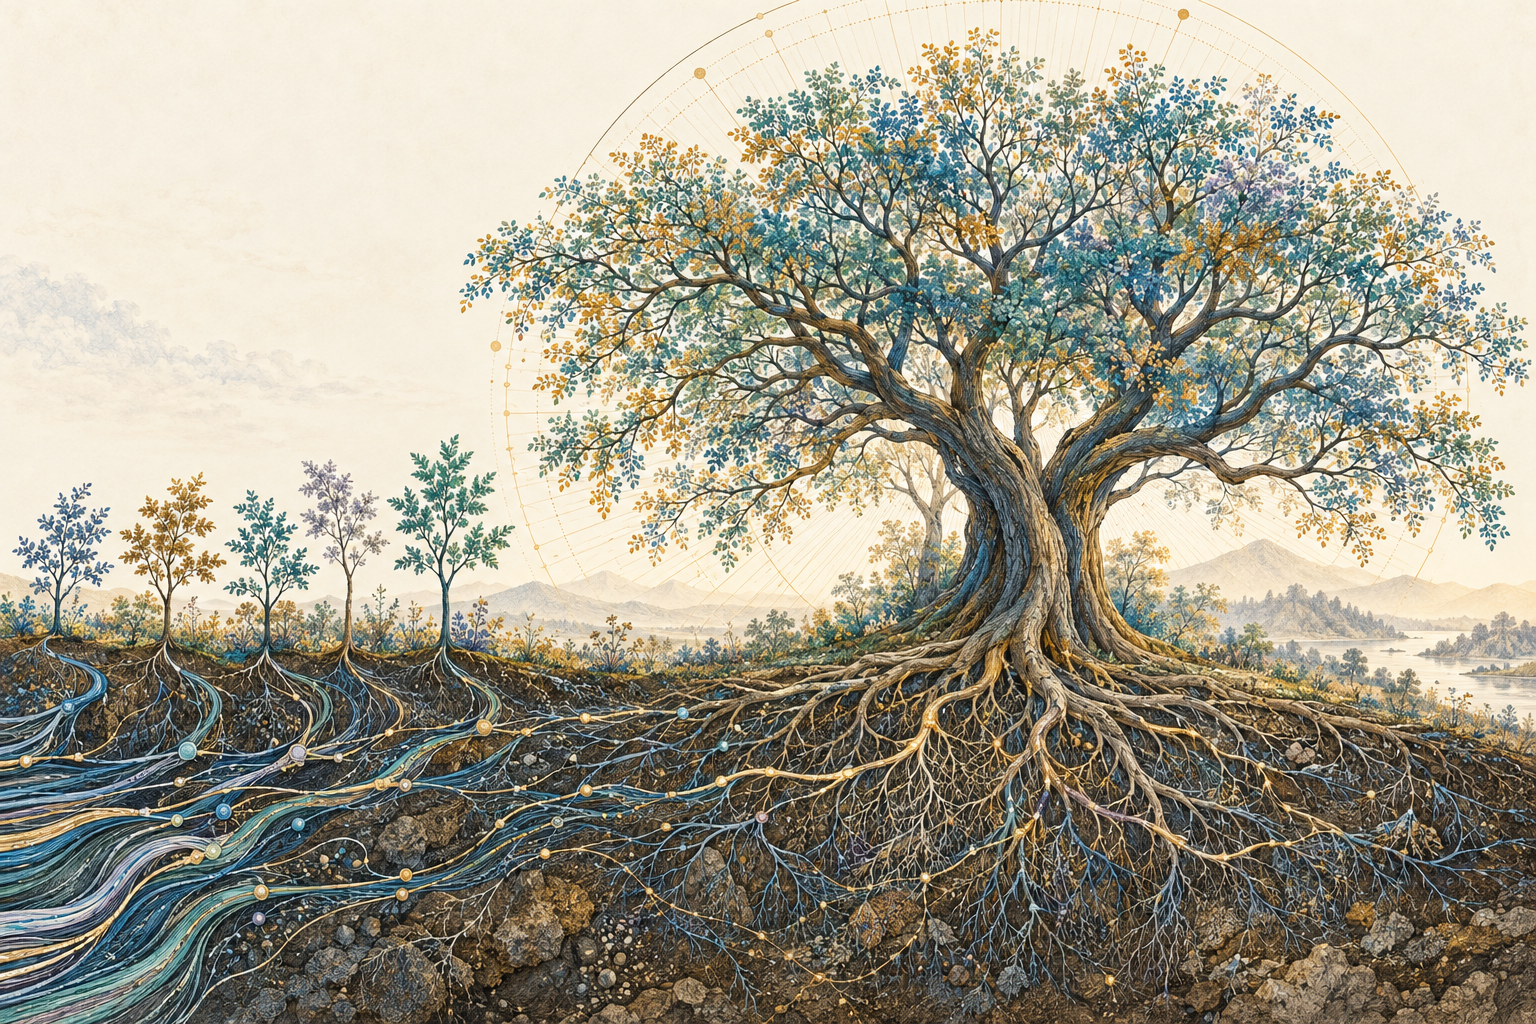
\includegraphics[width=\paperwidth]{figures/frontmatter/cover-d-commons-art.png}};
\draw[HeadingInk,line width=.55pt] ($(current page.north west)+(0mm,-112mm)$)--($(current page.north east)+(0mm,-112mm)$);
\draw[HeadingInk,line width=.55pt] ($(current page.north west)+(0mm,-252mm)$)--($(current page.north east)+(0mm,-252mm)$);
% Publisher wordmark only; original cover artwork and typography preserved.
\begin{scope}[blend mode=multiply]
\node[inner sep=0] at ($(current page.south)+(0mm,32mm)$)
{\includegraphics[width=36mm,trim=131.25bp 87.75bp 141bp 19.5bp,clip]{figures/frontmatter/cover-d2-assets/bcpress.pdf}};
\end{scope}
\node[anchor=south,inner sep=0,text=HeadingInk,font=\rmfamily\fontsize{13}{16}\selectfont]
at ($(current page.south)+(0mm,17mm)$) {BenchCouncil Press};
\end{tikzpicture}\clearpage


\clearpage\thispagestyle{empty}
\pdfbookmark[0]{Title Page}{review.title}
\vspace*{20mm}
\begin{center}
{\color{HeadingInk}\rule{\textwidth}{.8pt}}\par\vspace{2mm}
{\color{FrameworkRule}\rule{\textwidth}{.35pt}}\par\vspace{9mm}
{\bfseries\fontsize{28}{33}\selectfont\color{HeadingInk}Open Source Evaluatology\par}
\vspace{4mm}
{\fontsize{17}{23}\selectfont Theory, Methods,\\and Empirical Studies\par}
\vspace{9mm}
{\color{FrameworkRule}\rule{\textwidth}{.35pt}}\par\vspace{2mm}
{\color{HeadingInk}\rule{\textwidth}{.8pt}}\par
\vspace{18mm}
{\fontsize{15}{18}\selectfont Authors\par}
\vspace{6mm}
{\fontsize{14}{22}\selectfont
Wei Wang\par Shengyu Zhao\par Fanyu Han\par Xiaoya Xia\par}
\vfill
{\fontsize{13}{18}\selectfont\BookPublisher\par Hong Kong\par\BookDate\par}
\vspace*{31mm}
\end{center}\clearpage

\clearpage\thispagestyle{empty}
\pdfbookmark[0]{Copyright and Publication Details}{review.copyright}
\vspace*{6mm}
\begingroup\setlength{\parindent}{0pt}\setlength{\parskip}{12pt}
Copyright \textcopyright\ 2026 by Wei Wang, Shengyu Zhao,\\
Fanyu Han, and Xiaoya Xia

All rights reserved. No part of this book may be reproduced, stored in a retrieval system, or transmitted in any form or by any means, electronic or mechanical, including photocopying and recording, without the prior written permission of the publisher, except for brief quotations in reviews or scholarly analysis.

Published by BenchCouncil Press, Inc.\\
Room 1911, Lee Garden One, 33 Hysan Avenue,\\
Causeway Bay, Hong Kong, 999077\\
\href{https://press.benchcouncil.org}{\color{FrameworkBlue}\texttt{https://press.benchcouncil.org}}

First edition (Edition 1.0), November 2026

ISBN: to be assigned
\endgroup
\clearpage

\frontmatter
\hypersetup{pageanchor=true}
\begingroup
\XeTeXlinebreaklocale "zh"
\XeTeXlinebreakskip=0pt plus .15em
\ChineseBody\fontsize{11}{19}\selectfont
\setlength{\parindent}{2em}\setlength{\parskip}{3pt plus .3pt}
\thispagestyle{opening}
\pdfbookmark[0]{作者自序：从开源社区到开源评价学}{origins.zh}
\phantomsection\label{origins:zh}
\markboth{Open Source Evaluatology}{Author\textquotesingle s Note · Chinese Original}
\noindent{\ChineseSans\fontsize{10}{14}\selectfont\color{FrameworkTeal}写在前面\quad /\quad 中文原文}\par
\vspace{10pt}
\noindent{\ChineseSans\fontsize{23}{31}\selectfont\color{HeadingInk}从开源社区到开源评价学}\par
\vspace{17pt}
% Paragraph 01
我开始使用开源软件，远早于我开始理解开源社区。本科时，Linux、Apache、Tomcat 就已经出现在我的学习和实践中。那时，我最直接的感受是这些软件好用、开放，遇到问题可以查文档、读代码。至于谁在维护它们，陌生人如何合作，一个项目为什么能够延续多年，我还没有认真想过。

% Paragraph 02
2017年的中国开源年会，让这些熟悉的软件名字有了另一层意义。我第一次真正接触到项目背后的人和社区。有人写代码，有人组织协作，有人帮助新人，也有人长期承担很少被外界注意的维护工作。开源开始从一组软件名称，变成我能够感受到的人与人之间的联系。后来回望，这次相遇是我走向开源研究的一个重要起点。

% Paragraph 03
此后，由于个人原因，我调整了工作，来到华东师范大学数据科学与工程学院。新的环境也带来了一个很实际的问题：在一个数据学院里，怎样开展开源教学和科研？兴趣需要找到可以长期投入的方向，社区中的观察也需要转化为能够研究、能够验证的问题。我逐渐意识到，开源协作留下的大量公开记录，恰好为数据科学提供了一个丰富而真实的研究场景。

% Paragraph 04
赵生宇的加入，是这段探索中很重要的一步。我们相识于开源社区。他从阿里巴巴开源办公室离开，得知我正在组建开源研究团队，便来到我这里攻读博士。我们有共同的兴趣，也带着不同的经验：社区实践让研究问题有了来处，学术训练则要求我们把问题说清楚，把证据做扎实。团队就这样一点点组织起来。

% Paragraph 05
2020年，我们发布了《GitHub 2019 数字年报》。围绕2019年约5.46亿条 GitHub 公开事件日志，我们尝试描绘开发者、项目和组织的活动，也观察中国开源参与者在全球协作中的位置。对我们而言，这是第一次比较系统地用数据呈现开源生态。报告获得的关注和肯定，给了这个年轻团队很大的鼓励，也让我们看到，社区和产业确实需要这样的观察能力。同年，生宇还发表了《开源点亮未来》一文。“开源点亮未来”也由此成为我们实验室一直沿用的口号。

% Paragraph 06
随着报告传播，我们也开始考虑，怎样把一次分析积累下来的能力保留下来。数据怎样采集和整理，指标怎样定义，计算过程怎样复现，结果怎样持续更新，这些工作都值得开放出来。我们将制作报告的过程与方法逐步整理成一个开源项目，这便是 OpenDigger 的由来。从一份报告走向可以共同维护的数据基础设施，我们对开源世界的研究也有了能够持续生长的依托。

% Paragraph 07
2021年，OpenDigger 进入中国电子技术标准化研究院推动的木兰开源社区孵化，随后逐步为国家有关部门和机构提供开源数据服务。它的使用场景也不断扩大，陆续支持了开源社的《中国开源年度报告》、思否的《中国开源码力榜》、中国开源软件推进联盟的《中国开源发展蓝皮书》，以及 InfoQ 的开源发展研究分析。每一次合作，都使我们更具体地理解：不同使用者需要的证据，并不完全相同。

% Paragraph 08
围绕 OpenDigger，我们与合作伙伴逐渐建设起一组生态项目：OpenLeaderboard 帮助人们浏览和比较，HyperCRX 把数据带到日常使用的代码托管界面，OpenGalaxy 让协作关系有了直观的空间形态；与开放原子开源基金会共建的 OpenSODA 大赛、与蚂蚁共建的 OSGraph、与湖北大学共建的 OpenTalent，则把这些能力带入数据创新、关系探索和人才培养等场景。许多新的研究问题，正是从这些具体使用中长出来的。

% Paragraph 09
工具越是被使用，我们就越不能回避指标背后的问题。一个人做了多少事，与这些事产生了怎样的影响，究竟是什么关系？某个项目的活跃度下降，应当怎样理解？一个排名能够帮助谁，又可能遗漏谁？这些问题很难单靠增加数据量来回答。活跃度研究、OpenRank 算法家族和后续实证工作，使我们不断向前推进，也不断提醒我们审视测量的含义和边界。

% Paragraph 10
也正是在这样的探索中，我与詹剑锋教授的交流逐渐深入。我们最早相识于他发起的 BenchCouncil 系列活动。2022年11月，我们举办了首届国际开源软件生态基准论坛，此后每年都深入参与 Bench 大会。开源研究中的数据、指标和应用问题，在这里与基准、测量和评价方法的讨论交汇起来。

% Paragraph 11
詹教授对评价学的探索，让我重新审视我们已经做过的工作。过去，我们往往从一项数据或一个应用出发，寻找合适的方法；评价学则促使我们进一步说明，评价的对象是什么，在什么条件下比较，关注谁所受到的影响，又依据什么作出价值判断。那些分散在算法、平台和案例中的问题，开始有了可以贯通起来的理论线索。

% Paragraph 12
2024年12月，在广州举行的 Bench 大会上，我作了关于开源评价学的主题报告，华东师范大学也获授首个国际（开源）评价科学与工程研究中心。对我们而言，这是多年实践与评价学理论进一步结合的一个节点。开源评价学由此有了更明确的研究定位：以评价学为理论基础，系统研究开放协作中的贡献、影响、价值及其评价方法。

% Paragraph 13
我尤其看重其中的双向关系。理论帮助我们发现原先没有说清楚的假设，实践则让我们知道，哪些概念需要细化，哪些方法需要修正。比如，社区中长期的维护和协调工作，是否在指标中得到恰当体现；同一套评价用于不同组织时，结果还能否作相同解释；评价公布后，人们的行为又会发生怎样的变化。把这些问题带回理论，才有可能让领域研究与基础研究相互促进。

% Paragraph 14
2025年 Bench 大会前后，《Evaluatology: The Science of Uncovering the Effects》英文专著正式发布，中文版也于近期面世。在詹教授的持续推动下，我看到 BenchCouncil 从会议交流逐步发展出期刊、专著、基准平台等相互支撑的学术生态。一个方向要走得长远，需要有人提出问题，也需要可以积累知识、讨论分歧和检验方法的共同空间。这给了我们很大的启发。

% Paragraph 15
这本《开源评价学：理论、方法与实证》，就是在这样的背景下逐步成形的。写作使我们重新整理多年的论文、博士学位论文、工具和应用案例，也要求我们回答一个更难的问题：它们为什么属于同一个研究方向？从理论基础到测量方法，从实证研究到智库应用与学科建设，全书四个部分尝试给出连贯的回答。我们希望读者既能理解一项方法怎样工作，也能判断它适合回答什么问题。

% Paragraph 16
从实践中总结理论，是一项需要克制的工作。我们自己的案例可以提供证据，却不能替所有开源社区发言；某项算法在已有数据上的有效性，也不能自动延伸为对一切情境的解释。写这本书，是为了把依据、方法和局限交代得更清楚，让后来者能够继续检验和推进。开源评价学的体系，需要在这样的积累中逐步站稳。

% Paragraph 17
共同完成本书的，除了生宇，还有我的两位博士生韩凡宇和夏小雅。小雅已经博士毕业，进入蚂蚁开源办公室工作，继续活跃在国际开源社区中；凡宇也预计于2027年完成博士学业。从社区相识，到共同研究，再到把长期积累写成一本书，这几位年轻人的成长始终与团队的发展交织在一起。能够与他们共同署名，是我作为老师很珍惜的一件事。

% Paragraph 18
当然，书上四个作者的名字，远不能代表全部参与者。实验室同学对数据、代码、实验和文稿的投入，学院同事的支持，业界伙伴与社区同仁提供的问题、反馈和合作机会，都是这项工作得以延续的条件。很多贡献并没有署名在封面上，却实实在在地留在了书中。谨在这里向所有同行者致谢。

% Paragraph 19
回望这些年，开源也帮助我回答了刚到数据学院时的那个问题。真实场景提出需求，应用推动方法创新，创新再回到场景中接受检验，并支持更长远的发展。“场景驱动应用、应用驱动创新、创新驱动发展”，在开源研究中有了具体的内容：一份报告可以催生一个数据项目，一个工具可以进入课程和社区，一个实践中的疑问又可以成为新的研究课题。教学、科研与服务因此有了相互连接的路径。

% Paragraph 20
我们由此为开发者、企业、社区、基金会和政府机构提供了数据与评价服务，也在这个过程中培养了约三十位青年人才。他们走向不同的岗位，有人继续做研究，有人进入产业与社区。对一个大学实验室来说，能够留下可被使用的成果，也能够培养愿意参与公共协作的人，是很实在的收获。

% Paragraph 21
这些探索也发生在中国开源不断发展的背景下。开源已经写入“十四五”和“十五五”规划纲要，从支持开源社区到推进开源体系建设，其公共意义日益清晰。以 DeepSeek（深度求索）等为代表的开放实践，又让更多人看到，中国的技术团队可以通过分享成果，吸引全球开发者参与，建立跨越地域的合作联系。作为研究者，我们有机会参与其中，也有责任帮助人们更准确地理解这些变化。

% Paragraph 22
2026年7月9日，在瑞士日内瓦举行的“人工智能向善”（AI for Good）全球峰会边会上，我代表中国科协联合国咨商开源创新专委会（CCOSI），参与发布《2026全球开源发展报告》（预览版）。报告引起的关注与交流，让我感受到，开源数据研究已经可以服务于更广泛的国际对话。从2019年 GitHub 数据的整理，到面向全球开源发展的报告，研究的范围在扩大，最初想要理解协作的愿望一直没有变。

% Paragraph 23
全球对话也让评价的责任更加具体。不同地区的参与条件不同，不同社区留下的数据也不一样。一个看似整齐的比较，可能掩盖重要的差异。我们希望科学的评价能够帮助人们理解贡献、识别需要支持的地方，并为合作提供可信的依据。让开放成果更容易被使用，让长期维护和公共贡献得到更恰当的认识，是这项研究值得继续做下去的理由。

% Paragraph 24
今天，人工智能的发展使这些问题更加迫切。更多人能够获得技术，并不意味着每个人都拥有同样的参与机会。如何让不同背景的开发者进入协作，如何让有价值的公共成果得到持续支持，如何让技术进步惠及更广泛的人群，仍然需要长期工作。我期待开源评价学能在其中贡献一种扎实的研究方式，使关于开放与普惠的愿望，有可以讨论、可以检验、可以改进的依据。

% Paragraph 25
这本书面向国际读者，以英文写作。我仍想用中文留下这段缘起，并附上英文译文。中文是我们几位作者共同的母语，也承载着我们理解世界、交流想法和表达感谢的许多细节。保留它，是希望读者在概念、模型和图表之外，也能看见这项工作从什么地方出发，与哪些人相遇，又为什么坚持到了今天。

% Paragraph 26
从最初使用开源软件，到走进社区，再到与同行共同探索开源评价学，一路走来，最重要的始终是人与人的相遇，以及由此生长出的共同工作。愿这本书成为其中的一份贡献。也愿更多读者从这里接着往前走，让开放协作的价值被更好地理解，让愿意参与的人得到更多机会，让我们共同依赖的开源生态继续生长。

\par\vspace{12pt}\begin{flushright}\ChineseBody 王伟\\2026年11月，上海\end{flushright}
\clearpage\endgroup

\begingroup
\XeTeXlinebreaklocale "en"
\normalfont\fontsize{11}{13}\selectfont
\setlength{\parskip}{1pt plus .3pt}
\thispagestyle{opening}
\pdfbookmark[0]{Author\textquotesingle s Note: English Translation}{origins.en}
\phantomsection\label{origins:en}
\markboth{Open Source Evaluatology}{Author\textquotesingle s Note · English Translation}
\noindent{\sffamily\fontsize{10}{14}\selectfont\color{FrameworkTeal}AUTHOR\textquotesingle S NOTE\quad /\quad ENGLISH TRANSLATION}\par
\vspace{10pt}
\noindent{\sffamily\bfseries\fontsize{24}{29}\selectfont\color{HeadingInk}From Open Source Communities\\to Open Source Evaluatology}\par
\vspace{17pt}
% Paragraph 01
I began using open source software long before I began to understand open source communities. As an undergraduate, I was already using Linux, Apache, and Tomcat in my studies and practical work. What struck me then was their usefulness and openness: when I encountered a problem, I could consult the documentation or read the code. I had not yet thought seriously about who maintained these systems, how strangers managed to work together, or what enabled a project to endure.

% Paragraph 02
The China Open Source Conference in 2017 gave those familiar software names another meaning. For the first time, I came into real contact with the people and communities behind the projects. Some wrote code; others organized collaboration, helped newcomers, or carried out maintenance that received little attention beyond the community. Open source began to take shape for me as a network of human relationships. Looking back, that encounter was an important starting point for my research.

% Paragraph 03
Later, a change in my personal circumstances led me to move to the School of Data Science and Engineering at East China Normal University. The new setting brought a practical question: how should we teach and study open source within a school of data science? An interest had to become a direction worth sustained effort, and observations made in communities had to become questions we could investigate and test. I gradually came to see the public records of open collaboration as a rich, real setting for data science.

% Paragraph 04
Shengyu Zhao's arrival was an important step in this exploration. We had met through the open source community. After leaving Alibaba's Open Source Office, he learned that I was forming an open source research team and came to pursue his doctorate under my supervision. We shared an interest and brought different experiences. Community practice gave our questions a starting point, while academic research required us to formulate them clearly and establish sound evidence. The team took shape gradually.

% Paragraph 05
In 2020, we released the GitHub 2019 Digital Annual Report. Working with approximately 546 million public GitHub event records from 2019, we examined the activities of developers, projects, and organizations, including the place of Chinese participants in global collaboration. This was our first systematic attempt to describe the open source ecosystem through data. The attention and positive response encouraged our young team and showed us that communities and industry had a real need for this kind of observation. In the same year, Shengyu published a blog post titled “Open Source Lights Up the Future.” Its title became our laboratory’s enduring motto.

% Paragraph 06
As the report circulated, we began to consider how to preserve the capabilities developed through that analysis. Data collection and preparation, metric definitions, reproducible computation, and continuing updates were all worth making openly available. We gradually organized the report's processes and methods into an open source project. This was the origin of OpenDigger. Moving from a single report toward data infrastructure that others could help maintain gave our research a basis for continued growth.

% Paragraph 07
In 2021, OpenDigger entered incubation in the Mulan open source community, supported by the China Electronics Standardization Institute. It subsequently began providing open source data services to national departments and institutions. Its applications expanded to support Kaiyuanshe's China Open Source Annual Report, SegmentFault's Hacking Force China rankings, the China Open Source Development Blue Book led by the China Open Source Software Promotion Union, and InfoQ's research on open source development. Each collaboration helped us understand more precisely how the evidence required by one user could differ from that needed by another.

% Paragraph 08
Together with our partners, we gradually developed an ecosystem around OpenDigger. OpenLeaderboard supported browsing and comparison; HyperCRX brought data into the code-hosting interfaces people used every day; and OpenGalaxy gave collaboration networks a spatial form that could be explored visually. The OpenSODA competition, developed with the OpenAtom Foundation, OSGraph with Ant, and OpenTalent with Hubei University brought these capabilities into data innovation, relationship exploration, and talent development. Many new research questions grew out of these concrete uses.

% Paragraph 09
The more our tools were used, the harder it became to avoid the questions behind their metrics. How does the amount of work a person performs relate to its effects? How should a decline in a project's activity be interpreted? Whom can a ranking help, and whom might it overlook? More data alone cannot readily answer these questions. Our activity studies, the OpenRank family of algorithms, and subsequent empirical work moved us forward while repeatedly requiring us to examine what our measures meant and where their limits lay.

% Paragraph 10
During this period of exploration, my exchanges with Professor Jianfeng Zhan deepened. We had first met through the BenchCouncil activities he initiated. In November 2022, we held the first International Forum on Open Source Software Ecosystem Benchmarking, and we have participated closely in the Bench conference each year since. Questions about data, metrics, and applications in open source came into conversation there with research on benchmarks, measurement, and evaluation methods.

% Paragraph 11
Professor Zhan's work on Evaluatology prompted me to reconsider what we had already done. We had often started with a dataset or an application and sought an appropriate method. Evaluatology pressed us to make further questions explicit: what is being evaluated, under what conditions is a comparison made, whose experience of the effects matters, and on what basis is value judged? Questions dispersed across algorithms, platforms, and cases began to acquire a connecting theoretical thread.

% Paragraph 12
At the Bench conference in Guangzhou in December 2024, I delivered a keynote on Open Source Evaluatology, and ECNU received the designation of the first International Research Center for (Open Source) Evaluation Science and Engineering. For us, this marked a further connection between years of practice and the theory of Evaluatology. Open Source Evaluatology acquired a clearer research identity: a domain grounded in Evaluatology that systematically investigates contribution, influence, value, and their evaluation in open collaboration.

% Paragraph 13
I particularly value the two-way relationship. Theory helps us identify assumptions that we had left implicit; practice shows us which concepts need refinement and which methods need revision. Does a metric adequately represent sustained maintenance and coordination? Can the same interpretation be retained when an evaluation is used in different organizations? How might people change their behavior after an evaluation is published? Bringing such questions back to theory creates opportunities for domain research and foundational inquiry to advance together.

% Paragraph 14
Around the time of Bench 2025, the English monograph Evaluatology: The Science of Uncovering the Effects was released; a Chinese edition has appeared more recently. Through Professor Zhan's sustained efforts, I have seen BenchCouncil grow from a venue for conference exchange into an academic ecosystem supported by journals, monographs, and benchmark platforms. A field needs people who pose questions, and it also needs shared settings in which knowledge can accumulate, disagreements can be discussed, and methods can be tested. This development has been an important source of inspiration for us.

% Paragraph 15
Open Source Evaluatology: Theory, Methods, and Empirical Studies took shape in this setting. Writing it required us to revisit years of papers, doctoral dissertations, tools, and applications. It also required an answer to a harder question: why do these achievements belong to a single research field? Across four parts, from theoretical foundations and measurement methods to empirical studies, think-tank applications, and disciplinary development, the book attempts a coherent answer. We want readers to understand how a method works and to judge which questions it is suited to answering.

% Paragraph 16
Developing theory from practice requires restraint. Our cases can provide evidence, but they cannot speak for every open source community. An algorithm's performance on the data available to us does not automatically establish its explanatory power in every setting. We have written this book to make the evidence, methods, and limitations clearer, so that others can examine and extend the work. This is how we hope the foundations of Open Source Evaluatology will become stronger.

% Paragraph 17
My coauthors are Shengyu Zhao and two other doctoral students of mine, Fanyu Han and Xiaoya Xia. Xiaoya has completed her doctorate and joined Ant's Open Source Office, continuing her active engagement in international open source communities. Fanyu is expected to complete his doctorate in 2027. From encounters in the community to shared research and the writing of this book, their growth has been intertwined with that of the team. Being able to share authorship with them is something I deeply value as a teacher.

% Paragraph 18
The four names on the cover cannot represent everyone who has contributed. Students' work on data, code, experiments, and manuscripts; support from colleagues in the school; and the questions, feedback, and opportunities offered by industry partners and community members have all made this sustained effort possible. Many contributions have no name on the cover but remain present in the book. I offer my sincere thanks to everyone who has accompanied us.

% Paragraph 19
Looking back, open source has also helped me answer the question I faced on arriving at a school of data science. Real settings generate needs; applications drive methodological innovation; and innovations return to those settings to be tested and to support further development. The principle that “scenarios drive applications, applications drive innovation, and innovation drives development” has acquired concrete meaning in our work. A report can give rise to a data project, a tool can enter a course or a community, and a question from practice can become a research topic. Teaching, research, and service have found ways to connect.

% Paragraph 20
Through this work, we have provided data and evaluation services to developers, companies, communities, foundations, and government institutions, while helping to educate around thirty young professionals. They have taken different paths, continuing in research or moving into industry and community work. For a university laboratory, producing work that others can use and educating people willing to contribute to shared endeavors are tangible achievements.

% Paragraph 21
Our work has unfolded alongside the development of open source in China. Open source is included in both the Fourteenth and Fifteenth Five-Year Plans, with attention extending from support for communities to the development of an open source ecosystem. Its public significance has become increasingly clear. Open releases by teams such as DeepSeek have also shown how Chinese technology teams can share their work, attract participation from developers worldwide, and build relationships across geographical boundaries. As researchers, we have an opportunity to take part and a responsibility to help make these changes better understood.

% Paragraph 22
On 9 July 2026, at a side event of the AI for Good Global Summit in Geneva, Switzerland, I represented the CAST UN Consultative Committee on Open Source and Innovation (CCOSI) in the release of the 2026 Global Open Source Development Report, Preview Edition. The interest and discussion around the report brought home to me how open source data research could serve a broader international conversation. From analyzing GitHub data for 2019 to preparing a report on global open source development, the scope of our research has expanded. The original wish to understand collaboration has remained.

% Paragraph 23
International dialogue also makes the responsibilities of evaluation more concrete. Conditions of participation differ across regions, and communities leave different kinds of data. An apparently orderly comparison may conceal consequential differences. We hope that scientifically grounded evaluation can help people understand contributions, identify where support is needed, and establish a trustworthy basis for collaboration. Making open work easier to use, and improving the recognition of sustained maintenance and contributions to the public good, are reasons to continue this research.

% Paragraph 24
The development of artificial intelligence makes these questions more pressing. Wider access to technology does not give everyone the same opportunities to participate. Enabling developers from different backgrounds to join collaborative work, sustaining valuable public resources, and extending the benefits of technological progress all require sustained effort. I hope Open Source Evaluatology can contribute a sound way of investigating these questions, giving aspirations for openness and inclusion a basis that can be discussed, tested, and improved.

% Paragraph 25
This book is written in English for an international readership. I nevertheless wanted to record its origins in Chinese and provide an English translation. Chinese is the mother tongue of all four authors. It carries many of the details through which we understand the world, exchange ideas, and express gratitude. Keeping the original is a way of allowing readers to see, alongside the concepts, models, and figures, where this work began, whom we encountered, and why we have continued.

% Paragraph 26
From first using open source software to joining its communities and exploring Open Source Evaluatology with colleagues, what has mattered most has been meeting people and developing shared work from those encounters. I hope this book can make a contribution to that continuing effort. I also hope its readers will carry the work further: helping the value of open collaboration to be better understood, creating more opportunities for those who wish to participate, and sustaining the growth of the open source ecosystem on which we all depend.

\par\vspace{6pt}{\raggedleft\sffamily\fontsize{10}{13}\selectfont Wei Wang\quad Shanghai, November 2026\par}
\clearpage\endgroup
% Restore the original English book line-breaking behavior after bilingual matter.
\XeTeXlinebreaklocale ""

\chapter*{Preface}
\pdfbookmark[0]{Preface}{review.preface}
\label{review:preface}
\markboth{Open Source Evaluatology}{Preface}
A contribution to open source rarely ends where it is recorded. A patch may enter a library used by other projects. A careful review may prevent a failure that never appears in an issue tracker. A maintainer may help a newcomer whose most consequential work appears years later, elsewhere. These activities leave unequal traces. Their effects travel through technical dependencies and human relationships, and their value depends on who experiences them.

Evaluation enters this setting whenever someone must decide what deserves recognition, adoption, attention, or support. A contributor wants their work to be understood. A maintainer must distribute limited review time. An organization needs to understand the components on which it depends. A foundation must decide where assistance can sustain a shared capability. Each question calls for evidence, but the same observation does not carry the same meaning in every decision.

\emph{Open Source Evaluatology: Theory, Methods, and Empirical Studies} develops a foundation for investigating these questions. We establish Open Source Evaluatology as a domain of Evaluatology, grounded in open collaboration and connected to its practice. The parent discipline supplies concepts for examining objects, conditions, references, effects, and value. Open source gives these concepts a setting in which production crosses organizational boundaries, artifacts are widely reused, and benefits and maintenance obligations may fall on different parties.

The book grows out of a sustained programme of research. Activity studies made forms of participation visible and examined the distribution of collaborative work. OpenRank developed a relational account of influence and contribution. OpenDigger made observation, classification, and computation reusable. Contribution-recognition deployments brought evaluation into community practice, where its consequences could themselves be studied. Two doctoral dissertations provide much of the extended theoretical, technical, and empirical work behind these contributions. Our position paper connected this programme to Evaluatology; this monograph develops that connection into a systematic account.

The task is to explain how these achievements belong together. A descriptive measure needs an account of what it represents. A relational model needs a reason for its graph construction. An evaluation used in a course, community, or institution needs evidence about the purposes it serves and the consequences it creates. Tool development makes these inquiries practicable, while shared benchmarks and interdisciplinary research help examine the claims that follow. The book brings these responsibilities into one field without treating them as interchangeable.

Theory and practice work in both directions. Evaluatology guides the choice of object, conditions, comparison, and value. Empirical findings can require those choices to be reconsidered. Neglected coordination work changes the account of contribution. A maintained successor to an archived project changes the boundary of continuity. A public ranking can change the participation it represents. An institutional report can reveal a question that the available indicators cannot answer. Such findings contribute to theory as well as to an immediate application.

The eleven chapters develop this argument in four parts. Part I, \emph{Theory}, establishes the inquiry. Chapter 1 defines the domain and its foundations in Evaluatology. Chapter 2 examines collective capability, stakeholder effects, sustainability, and the consequences of evaluation. Chapter 3 turns these concepts into an evaluation-system design and relates it to completed studies.

Part II, \emph{Methods}, develops the means of inquiry. Chapter 4 examines Activity, from collaboration records and definitions to aggregation and empirical patterns. Chapter 5 develops OpenRank's global and community constructions, their validation, and the interpretation of relational scores. Chapter 6 explains OpenDigger and follows scalable computation and contribution recognition into use. Experiments and deployments establish the methods' capabilities and their limits.

Part III, \emph{Empirical Studies}, examines how the question changes with the setting. Chapter 7 studies contribution recognition through educational deployments. Chapter 8 investigates community sustainability through archival, maintenance, exit, transfer, and renewal. Chapter 9 examines ecosystem governance through Redis and Valkey, organizational contributions, and attribution. Together, the cases connect judgments about a person's work, a continuing capability, and an institutional arrangement.

Part IV, \emph{Applications and Disciplinary Development}, connects these findings to institutions and shared research practice. Chapter 10 develops open source think-tank applications through the global development report, observatories, and OpenDipper. Chapter 11 organizes the disciplinary framework, the open tool ecosystem, OpenPerf's benchmark comparisons, and the field's interdisciplinary foundations. It closes with research questions about comparability, visibility, reactivity, and revision, each grounded in the preceding evidence.

Three distinctions remain central throughout: recorded activity, relational influence, and stakeholder value; the evaluation of a measure and the evaluation of an arrangement that uses it; and reproducible computation and a justified interpretation. Each chapter develops its own question and references. Published results retain their populations, periods, units, and values. Current formulations guide the methodological exposition, while historical findings remain attached to the definitions that produced them. Proposed extensions are distinguished from completed studies.

We write for researchers and graduate students, and for maintainers, community leaders, educators, and institutional practitioners who need to examine the basis of an evaluation. Readers entering through a method can return to its assumptions in Part I; those entering through an application can trace its evidence to Part II. Open source software is the empirical centre of the book. Other forms of open collaboration require their own examination of production, rights, and affected parties.

Our aim is to make collaborative work intelligible, connect evidence to consequential choices, and learn from the consequences of those choices. The resulting foundation is intended to be used, examined, and revised.

\par\vspace{8pt}
{\raggedleft\sffamily\fontsize{10}{13}\selectfont\BookAuthors\par\BookDate\par}
\clearpage

% Generated by data/complete/build_contents.py.
\begingroup
\setlength{\parindent}{0pt}\setlength{\parskip}{0pt}
\newcommand{\booktocchapter}[3]{\par\vspace{11pt}{\sffamily\bfseries\fontsize{11.3}{14}\selectfont\color{HeadingInk}\noindent\begin{tabularx}{\linewidth}{@{}p{8mm}Xr@{}}\hyperref[#3]{#1}&\hyperref[#3]{#2}&\hyperref[#3]{\pageref*{#3}}\end{tabularx}}\par\vspace{6pt}}
\newcommand{\booktocsection}[3]{{\fontsize{9.8}{12}\selectfont\noindent\hyperref[#3]{\hspace*{8mm}\makebox[11mm][l]{#1}#2\nobreak\leaders\hbox{\kern1.5pt.\kern1.5pt}\hfill\nobreak\makebox[8mm][r]{\pageref*{#3}}}\par\vspace{4.5pt}}}

\chapter*{Contents}
\markboth{Open Source Evaluatology}{Contents}
\pdfbookmark[0]{Contents}{complete.contents}
\label{complete:contents}
\booktocsection{}{Author\textquotesingle s Note: Chinese Original}{origins:zh}
\booktocsection{}{Author\textquotesingle s Note: English Translation}{origins:en}
\booktocsection{}{Preface}{review:preface}
\booktocsection{}{Book Structure}{bookmap}
\vspace{5pt}
{\sffamily\bfseries\fontsize{13}{16}\selectfont\color{FrameworkTeal}\hyperref[part:1]{PART I\quad Theory\hfill\pageref*{part:1}}\par}
{\color{FrameworkTeal}\rule{\linewidth}{.55pt}}\par
\booktocchapter{1}{Foundations of Open Source Evaluatology}{ch:one}
\booktocsection{1.1}{The Evaluation Problem in Open Collaboration}{sec:growth}
\booktocsection{1.2}{Foundations in Evaluatology}{sec:foundations}
\booktocsection{1.3}{Open Collaboration as an Evaluation Domain}{sec:field}
\booktocsection{1.4}{From Measurements to Evaluative Claims}{sec:evidence}
\booktocsection{1.5}{Connecting Theory and Practice}{sec:intervention}
\booktocsection{1.6}{Research Questions and Scope}{sec:programme}
\booktocsection{}{References}{refs:chapter01}
\booktocchapter{2}{Value and Sustainability in Open Collaboration}{ch:two}
\booktocsection{2.1}{Activity, Contribution, and Collective Capability}{sec:production}
\booktocsection{2.2}{Influence and Recognition in Collaboration Networks}{sec:ch2-influence}
\booktocsection{2.3}{Effects, Stakeholders, and Value}{sec:stakeholders}
\booktocsection{2.4}{Time, Continuity, and Sustainability}{sec:continuity}
\booktocsection{2.5}{The Consequences of Evaluation}{sec:ch2-consequences}
\booktocsection{2.6}{Implications for Evaluation Design}{sec:value-theory}
\booktocsection{}{References}{refs:chapter02}
\booktocchapter{3}{A Framework for Open Source Evaluation}{ch:three}
\booktocsection{3.1}{Specify the Question and Intended Use}{sec:ch3-question}
\booktocsection{3.2}{Translate the Question into an Evaluation System}{sec:ch3-system}
\booktocsection{3.3}{Define Objects, Observations, and Measurements}{sec:ch3-evidence}
\booktocsection{3.4}{Select Models and Reference Conditions}{sec:ch3-models}
\booktocsection{3.5}{Plan Validation and Interpret Evidence}{sec:ch3-validity}
\booktocsection{3.6}{Three Completed Evaluation Designs}{sec:ch3-designs}
\booktocsection{}{References}{refs:chapter03}
\clearpage
\chapter*{Contents\enspace{\normalfont\sffamily\fontsize{13}{16}\selectfont continued}}
\markboth{Open Source Evaluatology}{Contents}
{\sffamily\bfseries\fontsize{13}{16}\selectfont\color{FrameworkBlue}\hyperref[part:2]{PART II\quad Methods\hfill\pageref*{part:2}}\par}
{\color{FrameworkBlue}\rule{\linewidth}{.55pt}}\par
\booktocchapter{4}{Measuring Activity in Open Collaboration}{ch:measurement}
\booktocsection{4.1}{Collaboration Events as Observations}{sec:ch4-observations}
\booktocsection{4.2}{Activity: Definitions and Aggregation}{sec:ch4-activity}
\booktocsection{4.3}{The 4WH Analytical Framework}{sec:ch4-framework}
\booktocsection{4.4}{Patterns of Collective Collaboration}{sec:ch4-patterns}
\booktocsection{4.5}{Aggregation Choices and Comparative Evidence}{sec:ch4-comparison}
\booktocsection{4.6}{Activity, Sustainability, and Evaluation}{sec:ch4-sustainability}
\booktocsection{}{References}{refs:chapter04}
\booktocchapter{5}{OpenRank: Influence and Contribution}{ch:five}
\booktocsection{5.1}{From Collaboration to Relational Evaluation}{sec:ch5-meaning}
\booktocsection{5.2}{The OpenRank Algorithm}{sec:ch5-formulation}
\booktocsection{5.3}{Global Influence across Repositories and Developers}{sec:ch5-global}
\booktocsection{5.4}{Contribution within a Community}{sec:ch5-community}
\booktocsection{5.5}{Validation across Models and Settings}{sec:ch5-evidence}
\booktocsection{5.6}{Interpreting Relational Scores}{sec:ch5-use}
\booktocsection{}{References}{refs:chapter05}
\booktocchapter{6}{OpenDigger: Evaluation in Practice}{ch:six}
\booktocsection{6.1}{Evaluation Requirements and System Design}{sec:ch6-system}
\booktocsection{6.2}{Data, Labels, and Observation Boundaries}{sec:ch6-observation}
\booktocsection{6.3}{Metric Services and Scalable Computation}{sec:ch6-services}
\booktocsection{6.4}{Validation of the Evaluation Infrastructure}{sec:ch6-validation}
\booktocsection{6.5}{Deploying Contribution Recognition}{sec:ch6-deployment}
\booktocsection{6.6}{Behavioural Feedback and Model Revision}{sec:ch6-feedback}
\booktocsection{}{References}{refs:chapter06}
\clearpage
\chapter*{Contents\enspace{\normalfont\sffamily\fontsize{13}{16}\selectfont continued}}
\markboth{Open Source Evaluatology}{Contents}
{\sffamily\bfseries\fontsize{13}{16}\selectfont\color{FrameworkAmber}\hyperref[part:3]{PART III\quad Empirical Studies\hfill\pageref*{part:3}}\par}
{\color{FrameworkAmber}\rule{\linewidth}{.55pt}}\par
\booktocsection{}{The Argument of Part III}{part3:guide}
\booktocchapter{7}{Recognizing Contributions in Open Collaboration}{ch:seven}
\booktocsection{7.1}{Contribution and the Purpose of Recognition}{sec:ch7-purpose}
\booktocsection{7.2}{Designing a Recognition System}{sec:ch7-design}
\booktocsection{7.3}{Evidence from Two Educational Deployments}{sec:ch7-evidence}
\booktocsection{7.4}{Relational Evidence and Contextual Judgment}{sec:ch7-agreement}
\booktocsection{7.5}{Feedback, Recourse, and Participation}{sec:ch7-feedback}
\booktocsection{7.6}{Validity and Consequences of Recognition}{sec:ch7-scope}
\booktocsection{}{References}{refs:chapter07}
\booktocchapter{8}{Evaluating Community Sustainability}{ch:sustainability}
\booktocsection{8.1}{Continuity beyond Repository Survival}{sec:ch8-continuity}
\booktocsection{8.2}{Designing the Archived-Project Study}{sec:ch8-study}
\booktocsection{8.3}{Why Projects Are Archived}{sec:ch8-reasons}
\booktocsection{8.4}{Development Trajectories and Maintenance Conditions}{sec:ch8-trajectories}
\booktocsection{8.5}{Exit, Transfer, and Renewal}{sec:ch8-exit}
\booktocsection{8.6}{Evaluating Continuity through Transition}{sec:ch8-assessment}
\booktocsection{}{References}{refs:chapter08}
\booktocchapter{9}{Evaluating Ecosystem Governance}{ch:governance}
\booktocsection{9.1}{Governance as an Evaluation Problem}{sec:ch9-question}
\booktocsection{9.2}{Observing the Redis Governance Transition}{sec:ch9-redis}
\booktocsection{9.3}{Organizational Contributions and Ecosystem Reconfiguration}{sec:ch9-reconfiguration}
\booktocsection{9.4}{Attribution across Organizations, Regions, and Fields}{sec:ch9-mapping}
\booktocsection{9.5}{From Evidence to Governance Judgments}{sec:ch9-judgment}
\booktocsection{9.6}{Accountability and Learning from Evaluation}{sec:ch9-accountability}
\booktocsection{}{References}{refs:chapter09}
\clearpage
\chapter*{Contents\enspace{\normalfont\sffamily\fontsize{13}{16}\selectfont continued}}
\markboth{Open Source Evaluatology}{Contents}
{\sffamily\bfseries\fontsize{13}{16}\selectfont\color{FrameworkViolet}\hyperref[part:4]{PART IV\quad Applications and Disciplinary Development\hfill\pageref*{part:4}}\par}
{\color{FrameworkViolet}\rule{\linewidth}{.55pt}}\par
\booktocsection{}{The Argument of Part IV}{part4:guide}
\booktocchapter{10}{Open Source Science and Technology Think Tanks}{ch:thinktanks}
\booktocsection{10.1}{From Evaluation to Decision Support}{sec:ch10-decision}
\booktocsection{10.2}{Goals, Indicators, and Observatory Design}{sec:ch10-observatory-design}
\booktocsection{10.3}{Mapping Global Open Source Development}{sec:ch10-global}
\booktocsection{10.4}{Regional and Organizational Applications}{sec:ch10-local}
\booktocsection{10.5}{Visual Investigation with OpenDipper}{sec:ch10-visual}
\booktocsection{10.6}{Knowledge Products and Institutional Use}{sec:ch10-products}
\booktocsection{}{References}{refs:chapter10}
\booktocchapter{11}{Disciplinary Development and the Tool Ecosystem}{ch:discipline}
\booktocsection{11.1}{A Framework for Disciplinary Development}{sec:ch11-framework}
\booktocsection{11.2}{An Open Evaluation Tool Ecosystem}{sec:ch11-ecosystem}
\booktocsection{11.3}{Tools for Evidence and Interpretation}{sec:ch11-interfaces}
\booktocsection{11.4}{Validation and Shared Benchmarks}{sec:ch11-benchmarks}
\booktocsection{11.5}{Interdisciplinary Foundations}{sec:ch11-interdisciplinary}
\booktocsection{11.6}{Building a Cumulative Research Programme}{sec:ch11-programme}
\booktocsection{}{References}{refs:chapter11}
\clearpage
\endgroup

% Approved architecture with linked chapter cells.
\chapter*{Book Structure}
\pdfbookmark[0]{Book Structure}{bookstructure.bookmark}
\label{bookmap}
\markboth{Open Source Evaluatology}{Book Structure}
\noindent Evaluatology supplies the foundation. Theory specifies the inquiry, methods construct its evidence, and empirical studies examine its use. Institutional applications and shared research practice return new requirements to this foundation.
\par\vspace{8pt}
\noindent\begin{tikzpicture}[x=1mm,y=1mm,
 cell/.style={sebox,text width=36mm,minimum height=21mm,font=\sffamily\fontsize{8.6}{10.2}\selectfont},
 band/.style={seband,text width=127mm,minimum height=8mm},
 result/.style={sebox,text width=127mm,minimum height=7mm,font=\sffamily\fontsize{8.3}{10}\selectfont}]
\node[band,minimum height=13mm] (base) at (65,0)
 {EVALUATOLOGY\\[-1pt]\normalfont\sffamily\fontsize{8.6}{10.2}\selectfont Objects and effects \quad$\cdot$\quad Conditions and comparison \quad$\cdot$\quad Value};
\node[band,fill=FrameworkTeal] (t) at (65,-17) {I\quad THEORY \hfill Define the domain and its inquiry};
\node[cell,fill=FrameworkTeal!12] (c1) at (21,-33) {\hyperref[ch:one]{\textbf{1}\\Foundations of Open\\Source Evaluatology}};
\node[cell,fill=FrameworkTeal!12] (c2) at (65,-33) {\hyperref[ch:two]{\textbf{2}\\Value and Sustainability\\in Open Collaboration}};
\node[cell,fill=FrameworkTeal!12] (c3) at (109,-33) {\hyperref[ch:three]{\textbf{3}\\A Framework for\\Open Source Evaluation}};
\node[result,fill=FrameworkTeal!6] (r1) at (65,-49) {Evaluation questions, collective capability, stakeholder effects, and research design};
\node[band,fill=FrameworkBlue] (m) at (65,-61) {II\quad METHODS \hfill Construct and examine the measures};
\node[cell,fill=FrameworkBlue!12] (c4) at (21,-77) {\hyperref[ch:measurement]{\textbf{4}\\Measuring Activity in\\Open Collaboration}};
\node[cell,fill=FrameworkBlue!12] (c5) at (65,-77) {\hyperref[ch:five]{\textbf{5}\\OpenRank: Influence\\and Contribution}};
\node[cell,fill=FrameworkBlue!12] (c6) at (109,-77) {\hyperref[ch:six]{\textbf{6}\\OpenDigger: Evaluation\\in Practice}};
\node[result,fill=FrameworkBlue!6] (r2) at (65,-93) {Measurements, relational models, infrastructure, and observed consequences};
\node[band,fill=FrameworkAmber] (e) at (65,-105) {III\quad EMPIRICAL STUDIES \hfill Examine evidence in use};
\node[cell,fill=FrameworkAmber!12] (c7) at (21,-121) {\hyperref[ch:seven]{\textbf{7}\\Recognizing Contributions\\in Open Collaboration}};
\node[cell,fill=FrameworkAmber!12] (c8) at (65,-121) {\hyperref[ch:sustainability]{\textbf{8}\\Evaluating Community\\Sustainability}};
\node[cell,fill=FrameworkAmber!12] (c9) at (109,-121) {\hyperref[ch:governance]{\textbf{9}\\Evaluating Ecosystem\\Governance}};
\node[result,fill=FrameworkAmber!6] (r3) at (65,-137) {Recognition and recourse \quad$\cdot$\quad Continuity through change \quad$\cdot$\quad Bounded judgment};
\node[band,fill=FrameworkViolet,minimum height=11mm] (v) at (65,-151)
 {IV\quad APPLICATIONS AND DISCIPLINARY DEVELOPMENT\\[-1pt]\normalfont\sffamily\fontsize{8.3}{10}\selectfont Connect institutional use with cumulative research};
\node[cell,text width=58mm,minimum height=18mm,fill=FrameworkViolet!7,draw=FrameworkViolet!60] (c10) at (32,-169) {\hyperref[ch:thinktanks]{\textbf{10}\\Open Source Science and\\Technology Think Tanks}};
\node[cell,text width=58mm,minimum height=18mm,fill=FrameworkViolet!7,draw=FrameworkViolet!60] (c11) at (98,-169) {\hyperref[ch:discipline]{\textbf{11}\\Disciplinary Development\\and the Tool Ecosystem}};
\draw[searrow] (base.south)--(t.north);
\draw[searrow] (r1.south)--(m.north);
\draw[searrow] (r2.south)--(e.north);
\draw[searrow] (r3.south)--(v.north);
\foreach \a/\b in {c1/c2,c2/c3,c4/c5,c5/c6,c7/c8,c8/c9,c10/c11} \draw[searrow] (\a.east)--(\b.west);
\draw[sefeedback,draw=FrameworkAmber] (r3.east)--(135,-137)--(135,-17)--(t.east);
\draw[sefeedback,draw=FrameworkViolet] (c11.east)--(139,-169)--(139,-61)--(m.east);
\end{tikzpicture}
\par\vspace{6pt}
\noindent{\sffamily\fontsize{9}{11.5}\selectfont\raggedright
\textbf{Figure P.1. Architecture of the book.}
Solid arrows mark the progression of the argument. Dashed arrows return empirical requirements to theory and lessons from applications and validation to methods. They indicate intellectual feedback, not estimated causal effects. Original conceptual diagram.\par}

\mainmatter
\clearpage
\BookChapterRunningfalse
\def\BookPartTitle{Theory}
\bookpart{I}{Theory}{FrameworkTeal}{36}
{What should an evaluation explain?}
{1}
{Evaluation begins with a question about collaborative work and its effects. The first part establishes the domain, examines value and continuity, and develops a framework for designing a defensible inquiry.}
{\reviewpartchapter{1}{Foundations of Open Source Evaluatology}{The domain and its foundations in Evaluatology}{FrameworkTeal}
\reviewpartchapter{2}{Value and Sustainability in Open Collaboration}{Collective capability, effects, and continuity}{FrameworkTeal}
\reviewpartchapter{3}{A Framework for Open Source Evaluation}{From a question to an evaluation system}{FrameworkTeal}}

\BookChapterRunningtrue
\begin{cbunit}
\chapter{Foundations of Open Source Evaluatology}
\label{ch:one}
\markboth{Open Source Evaluatology}{Foundations of the Field}

Open source collaboration makes a substantial part of software production observable. It does not make the significance of that production self-evident. A project can attract more activity while accumulating a larger maintenance burden. A widely reused component can receive little visible attention in its own repository. A contributor can improve the work of others through review, explanation, and coordination without producing the largest volume of code. Evaluation must explain which of these differences matters, under what conditions, and to whom.

This chapter establishes Open Source Evaluatology as a domain of Evaluatology. The parent discipline supplies an account of objects, conditions, causes and effects, and value. Our research on Activity, OpenRank, OpenDigger, and contribution recognition supplies methods and evidence through which that account can be developed for open collaboration. The aim is a cumulative field: concepts should guide empirical inquiry, and findings should be able to change those concepts and their operational realization.

The argument has three elements. An evaluation question must identify its object, affected parties, purpose, and reference. Measurements and models must be distinguished from the claims attached to their outputs. An evaluation arrangement can itself become an object of inquiry when its use changes collaboration. These elements provide the foundation for Chapter 2's account of value and sustainability and Chapter 3's research framework. Chapters 4--6 develop and examine the methods on which the synthesis rests.

\section{The Evaluation Problem in Open Collaboration}
\label{sec:growth}

\subsection{Three problems arising from the research}
The first problem is the visibility of useful work. In the OpenRank Leaderboard study, a selected maintainer's participation consisted largely of coordination across issues and pull requests. A commit-based ordering gave a different account from the community network measure \citep[Section 4.1]{zhao2024}. The disagreement asks a substantive question: what contribution is the evaluation intended to recognize? More records or a more elaborate algorithm cannot answer that question without an account of the work being represented.

The second problem concerns the organization of participation. Our Activity study examined who contributed, what they did, when participation occurred, and where it appeared across the collaboration landscape \citep{xia2022}. Its findings include concentrated participation, different mixes of human and automated behaviour, and temporal patterns. These are consequential observations, but their interpretation depends on the undertaking. Concentration can accompany expertise and continuity, or expose dependence on a small number of people. Distinguishing those possibilities requires evidence about responsibilities, substitutes, and the conditions of continued work.

The third problem appears when evaluation is put into use. Publishing a contribution ranking can change attention and behaviour. Participants in the leaderboard deployment reported changes in how they communicated and divided their work \citep[Section 4.2]{zhao2024}. Such responses can alter both collaboration and the public record through which collaboration is measured. The resulting inquiry has two objects: the representation of contribution and the arrangement that uses it. Evidence about the first does not settle the consequences of the second.

These problems explain the sequence of Part II. Chapter 4 establishes the observations and Activity measurements. Chapter 5 asks what a relational account adds and examines OpenRank. Chapter 6 supplies the infrastructure and follows evaluation into practice. The complete results belong there. In this chapter, the studies identify the conceptual commitments needed to understand those results and to ask further questions of them.

\subsection{From separate research traditions to a common question}
Research on open source already offers substantial accounts of collaboration. The Apache and Mozilla cases connected participation and work organization to software outcomes; a later review distinguished inputs, processes, emergent states, and outputs \citep{mockus2002,crowston2012}. Open superposition explains how independently motivated layers of work can enable subsequent contributions \citep{howison2014}. These studies make clear why the significance of an action often depends on work performed by others.

The pull-based development literature gives that observation a concrete workflow. Submission, discussion, integration, and rejection are different events, with different implications for an artifact and the people maintaining it \citep{gousios2014}. A submitted change can create review work without producing an accepted feature. A review can improve an artifact without adding a large volume of code. An evaluation must explain which stage it observes and which consequence it seeks to assess.

Our position paper began to organize such questions through Evaluatology's objects, conditions, and results \citep{han2024ose}. The present book develops that connection by retaining affected objects, reference alternatives, stakeholder purposes, and the consequences of use throughout the argument. It brings the domain framework into contact with the empirical and technical work on which the following chapters are built.

The resulting field has a common problem rather than a single preferred score. It asks how evidence about open collaboration can support a stated evaluative conclusion. A descriptive inquiry, a network comparison, and a deployment study can all contribute, provided their objects and interpretations remain explicit. Their conclusions become cumulative when the conditions under which they hold can be inspected and compared.

\section{Foundations in Evaluatology}
\label{sec:foundations}

\subsection{A shared system of inquiry}
The initial formulation of Evaluatology emphasized the science and engineering of evaluation and the dependence of results on evaluation conditions \citep{zhan2024}. The subsequent Chinese monograph develops a broader account centred on causes and effects and places Evaluatology within a proposed system of scientific inquiry \citep{zhan2026book}. We adopt its conceptual organization as a theoretical foundation while distinguishing that organization from the empirical evidence and method-specific assumptions needed in a particular study.

Figure~\ref{fig:disciplines} adapts the monograph's first foundational diagram. Metrology concerns the definition, realization, and assignment of structural and behavioural quantities. Testology concerns the testing of propositions and models, as well as behavioural quantities. Inferology concerns the generation of propositions and models. Evaluatology investigates causes and effects, with the narrower activity of valuation concerned with quantities of value. Their relationship is mutually supportive: a model can guide measurement, measurements can challenge a model, and an evaluative question can determine which behaviours require testing.

\begin{figure}[tbp]
\centering
\begin{tikzpicture}[x=1mm,y=1mm,
 d/.style={sebox,text width=28mm,inner sep=1.2mm,minimum height=32mm,
 font=\sffamily\fontsize{8.6}{10.3}\selectfont},
 top/.style={seband,text width=127mm,minimum height=13mm}]
\node[top] (f) at (66,0) {A SHARED FOUNDATION FOR SCIENTIFIC INQUIRY\\[-1pt]
 \normalfont\sffamily\fontsize{8.7}{10.3}\selectfont Basic concepts \quad$\cdot$\quad Axioms and conjectures};
\node[d,fill=FrameworkAmber!16,draw=FrameworkAmber!70] (m) at (16.5,-37) {};
\node[d,fill=FrameworkBlue!14,draw=FrameworkBlue!70] (t) at (49.5,-37) {};
\node[d,fill=FrameworkViolet!16,draw=FrameworkViolet!70] (e) at (82.5,-37) {};
\node[d,fill=FrameworkTeal!14,draw=FrameworkTeal!70] (i) at (115.5,-37) {};
\foreach \x/\title in {16.5/METROLOGY,49.5/TESTOLOGY,82.5/EVALUATOLOGY,115.5/INFEROLOGY}
 {\node[font=\sffamily\bfseries\fontsize{8.6}{10.3}\selectfont,text=HeadingInk] at (\x,-25) {\title};}
\node[selabel,text=HeadingInk,text width=28mm,anchor=north] at (16.5,-29)
 {Structural and\\behavioural quantities:\\definition, realization,\\and assignment};
\node[selabel,text=HeadingInk,text width=28mm,anchor=north] at (49.5,-29)
 {Testing propositions\\and models; behavioural\\quantities: definition,\\realization and assignment};
\node[selabel,text=HeadingInk,text width=28mm,anchor=north] at (82.5,-29)
 {Causes and effects;\\value quantities\\in the narrower\\sense of evaluation};
\node[selabel,text=HeadingInk,text width=28mm,anchor=north] at (115.5,-29)
 {Generation of\\new propositions\\and models};
\draw[draw=HeadingInk!85,line width=.65pt] (f.south)--(66,-13);
\draw[draw=HeadingInk!85,line width=.65pt] (16.5,-13)--(115.5,-13);
\foreach \x/\n in {16.5/m,49.5/t,82.5/e,115.5/i}
 {\draw[searrow] (\x,-13)--(\n.north);}
\draw[{Stealth[length=1mm]}-{Stealth[length=1mm]},draw=HeadingInk!85,line width=.55pt] (m.east)--(t.west);
\node[sebox,text width=127mm,minimum height=10mm,fill=HeadingInk!6] (r) at (66,-68)
 {Mutually supporting forms of inquiry};
\foreach \x/\n in {16.5/m,49.5/t,82.5/e,115.5/i}
 {\draw[searrow] (\n.south)--(\x,-63);}
\end{tikzpicture}
\caption{Four disciplines within a shared system of inquiry. English adaptation of \citet[Fig.~1.1, p.~3]{zhan2026book}. Shared concepts and axioms support four mutually reinforcing disciplines. Layout and wording are condensed; arrows express conceptual relationships.}
\label{fig:disciplines}
\end{figure}


For open collaboration, this arrangement clarifies the roles of familiar research activities. An operational definition of review latency is a measurement task. Checking the behaviour of a data-processing procedure is a testing task. Proposing that early review helps newcomers learn introduces a model of a relationship. Investigating whether a particular review arrangement changes subsequent participation is an evaluative task. The categories organize questions; a single empirical study may contain all four.

The conceptual hierarchy in Figure~\ref{fig:hierarchy} provides a second foundation. The general level supplies terms such as object, relationship, event, subject, proposition, and model. The disciplinary level gives these terms more specific roles. The methodological level introduces the assumptions and operations of particular approaches to evaluation. This hierarchy helps prevent a frequent error: moving from a general statement about causes to the conclusion that a selected statistical procedure identifies them.

\begin{figure}[tbp]
\centering
\begin{tikzpicture}[x=1mm,y=1mm,
 disc/.style={sebox,text width=27.5mm,minimum height=11mm},
 meth/.style={semethod,text width=60mm,minimum height=10mm}]
\node[seband,text width=127mm,minimum height=13mm] (b) at (66,0)
 {GENERAL CONCEPTS\\[-1pt]\normalfont\sffamily\fontsize{8.7}{10.3}\selectfont Objects, relationships, events, subjects, interrogation,\\cause and effect, propositions, models, axiom systems};
\node[disc,fill=FrameworkAmber!14] (a) at (16.5,-26) {\textbf{Metrology}};
\node[disc,fill=FrameworkBlue!13] (c) at (49.5,-26) {\textbf{Testology}};
\node[disc,fill=FrameworkViolet!18] (e) at (82.5,-26) {\textbf{Evaluatology}};
\node[disc,fill=FrameworkTeal!13] (i) at (115.5,-26) {\textbf{Inferology}};
\draw[searrow] (b.south)--(66,-14)--(16.5,-14)--(a.north);
\draw[searrow] (66,-14)--(49.5,-14)--(c.north);
\draw[searrow] (66,-14)--(82.5,-14)--(e.north);
\draw[searrow] (66,-14)--(115.5,-14)--(i.north);
\node[seband,text width=127mm,minimum height=8mm,fill=FrameworkViolet] (h) at (66,-44)
 {METHOD-SPECIFIC CONCEPTS AND ASSUMPTIONS};
\draw[searrow] (e.south)--(82.5,-40);
\node[meth] at (33,-58) {Object causal models};
\node[meth] at (99,-58) {Design of experiments};
\node[meth] at (33,-71) {Randomized controlled trials};
\node[meth] at (99,-71) {Potential outcomes theory};
\node[meth] at (33,-84) {Quasi-experiments};
\node[meth] at (99,-84) {Structural equation models};
\node[meth] at (33,-97) {Structural causal models};
\node[meth] at (99,-97) {Instrumental variables};
\end{tikzpicture}
\caption{From a shared vocabulary to disciplines and evaluation methods. Adapted from \citet[Fig.~1.2, p.~5; Section~1.3]{zhan2026book}. The nine general concepts are supplied from the accompanying text; all eight method families in the original figure are retained. Branches indicate conceptual specialization. The methods overlap and have different assumptions; the diagram assigns no common identification guarantee.}
\label{fig:hierarchy}
\end{figure}


The eight method families in the source diagram are retained. They are not disjoint classes or interchangeable solutions. Experimental design concerns how observations are generated; potential outcomes and structural causal models provide different formal resources for posing and identifying causal questions; instrumental variables is a method requiring particular assumptions. An object causal model is another proposed representation with its own definitions. A place in a common conceptual hierarchy does not remove these differences.

The value of this hierarchy for the present book is architectural. It allows a common vocabulary to connect chapters without requiring them to use a single estimation technique. A study of review practices and a study of package dependencies can share a definition of an evaluation question while requiring different observation models, comparisons, and validation procedures.

\subsection{Objects, systems, and conditions}
The monograph distinguishes an evaluated object (EO), affected objects (AOs), and other causally relevant objects, termed confounding objects (COs) in its framework \citep[Chapters~8 and 10]{zhan2026book}. These are roles relative to a question. A contributor can be the evaluated object in a recognition study and an affected object in a study of a mentoring programme. A repository is an artifact and an observation site; it does not automatically delimit the community or the relevant causal system.

The term CO requires care when used alongside statistical terminology. The monograph's object category concerns other objects that can influence the affected objects. It should not be equated without further argument with a confounder in a particular causal identification model. Whether an observed variable is a confounder, mediator, or consequence of selection depends on the question and the model. Translating an object-level account into a statistical design is substantive work.

The source further distinguishes a real-world system (RWS), a \emph{self-contained system} (SCS), and an \emph{object causal model} (OCM). An SCS is a physical experimental model containing the cause object, affected objects, and relevant objects that cannot be isolated. The evaluation condition (EC) is defined as the system remaining when the EO is removed. An OCM is a mathematical representation based on influence mechanisms among objects; it models a real-world or self-contained system and must be examined against observations or tests \citep[pp.~117--120]{zhan2026book}.

These distinctions are useful precisely because they make modelling commitments visible. A database assembled from public events is an observation product. A simulated collaboration network is a mathematical construction. Neither becomes an SCS merely by selecting a subset of repositories. In an open community, preserving the relevant mechanisms while isolating an intervention can be difficult: contributors may work across groups, reviewers may share knowledge, and changes may reach downstream users. The investigator must explain which relationships the study preserves and which it abstracts away.

An object-based account also helps formulate mechanisms. A mentoring arrangement may affect a newcomer's access to guidance; guidance may change the newcomer's capability; the resulting work may affect a review team and eventually a release. Each relation suggests observations and possible alternatives. The framework's role is to state those relations. Their existence and strength remain questions for the relevant evidence.

\subsection{Effects and value}
The parent monograph defines value through the consequences, for stakeholders, of differences between the effects of an object and those of a reference object \citep[Chapter~11]{zhan2026book}. This makes evaluation more demanding than attaching favourable labels to an activity. A change can improve one outcome and worsen another, and the parties affected need not agree on the importance of either. A maintainer may value fewer interruptions, a newcomer may value access to explanation, and a downstream organization may value predictable releases.

The private--collective innovation model and research on firms' open source strategies explain why shared artifacts can support different forms of benefit \citep{vonhippel2003,west2006}. Our framework carries this insight into evaluation by keeping stakeholder-specific consequences explicit.

The distinction between effects and value is consequently analytical rather than a separation of research from practice. Evidence about effects constrains what a value judgment can reasonably claim. Purposes and stakeholder commitments determine which effects should be investigated and how they enter a decision. Chapter 2 develops this relationship in detail. Here it supplies the basis for specifying the domain and its research questions.

\section{Open Collaboration as an Evaluation Domain}
\label{sec:field}

\subsection{A domain defined by objects and their relationships}
The position paper introduced project, developer, and community dimensions and combined statistical and network perspectives \citep{han2024ose}. These dimensions are useful points of entry. The relevant object, however, can also be an artifact, a process, an organizational arrangement, or a relationship among several communities. Its boundary follows the evaluation question.

\begin{definitionbox}
\textbf{Open Source Evaluatology} is the domain of inquiry that investigates the effects of objects and arrangements in open collaboration, evaluates the value of those effects under explicit conditions and purposes, and examines the consequences of evaluation itself.
\end{definitionbox}

A repository is a technical container and an observation site. A project organizes work on an artifact or a related set of artifacts. A community includes participants, practices, and governance whose boundaries may extend across repositories. An organization can participate in several communities, and an ecosystem connects undertakings through reuse, dependencies, shared people, and institutions. These terms identify different objects and levels; they should not become synonyms merely because a dataset offers one repository identifier per row.

The evaluated object can be located at one level while its effects occur at another. A component change can affect downstream applications. An organizational funding rule can alter the availability of maintainers across projects. A public recognition arrangement can affect the allocation of contributor effort. Ecosystem health research and studies of package dependencies demonstrate why an individual project's observations can omit relevant interdependencies \citep{jansen2014,decan2019}. Enlarging a boundary is useful when it includes relationships required by the question, rather than simply producing a larger graph.

Stakeholders and affected objects likewise have different roles. A patch may affect a library's behaviour; a service operator experiences consequences of using that library. In a learning-oriented community, the contributor can be both an affected object, through changed capability, and a stakeholder concerned with the value of that change. An evaluation should preserve these roles even when one entity occupies several of them.

\subsection{An explicit specification of the question}
We use the working specification
\begin{equation}
\mathcal Q=\langle O,A,C,R,T,S,P\rangle ,
\label{eq:question}
\end{equation}
where \(O\) is the evaluated object or arrangement; \(A\) identifies affected objects together with their outcome quantities; \(C\) specifies conditions; \(R\) is the reference alternative; \(T\) is the time horizon; \(S\) identifies stakeholders; and \(P\) states the purpose. This tuple is the book's organizing notation. It makes commitments inspectable and supplies no causal identification result by itself.

For a descriptive Activity inquiry, \(O\) may be the recorded participation of a declared group of projects. The reference can be another period or comparison population. The purpose may be to characterize the composition of work. Relevant affected objects and outcomes can be named without claiming that the description estimates an effect on them. For a contribution-recognition study, the evaluated object can instead be the public arrangement; contributors, maintainers, and collaborative processes become affected objects. The reference concerns an alternative arrangement, and the horizon must be long enough to observe the consequences being claimed.

A mentoring example shows how the same specification supports a different design. The arrangement assigns experienced reviewers to newcomers. The affected objects include newcomers and reviewers; relevant quantities include learning, continuing participation, and effort. The reference might be the existing review process. Research on sustained participation and newcomer barriers helps specify these mechanisms and outcomes \citep{fang2009,steinmacher2015}. Those findings inform the question without establishing the effect of the particular arrangement being proposed.

The conditions \(C\) include governance, eligibility, workload, platform affordances, and concurrent changes. They are broader than a set of regression covariates and should be distinguished from the specific evaluation-condition construction in Section~\ref{sec:foundations}. A data snapshot, identity rule, or algorithm version records how the question was realized. Changing such a rule can change a result even when community behaviour is unchanged. Chapter 3 makes these relationships operational through the five-component evaluation architecture.

The specification also identifies where disagreement lies. Researchers may disagree about the relevant community boundary, the interpretation of an outcome, the alternative against which it should be compared, or whose consequences matter. Those disagreements require different evidence and deliberation. Recording them explicitly helps prevent an apparently precise score from concealing an unresolved evaluation question.

\section{From Measurements to Evaluative Claims}
\label{sec:evidence}

\subsection{What a measurement establishes}
A measurement assigns a quantity under a specified procedure. The validity of a stronger interpretation depends on what that procedure represents. Software measurement research examines units, instrumentation, protocols, and populations; assessment theory examines the evidence supporting score meaning and use \citep{kitchenham1995,messick1995}. These perspectives direct attention to the connection between a calculation and the claim it is asked to support.

Activity measures recorded participation under a behaviour selection, attribution rule, period, transformation, and aggregation. A larger value establishes a difference under that specification. It does not by itself establish better software or a more sustainable division of work. The SPACE framework makes a related distinction in developer productivity: activity is one dimension within a broader account of work and experience \citep{forsgren2021}. In our setting, the intended collaborative function determines which additional evidence is needed.

OpenRank assigns influence or contribution through a specified graph and propagation model. Its score depends on the represented objects, relations, priors, and comparison population. Centrality research shows why an interpretation depends on the process that network connections are assumed to represent \citep{borgatti2005}. A relational score can make coordination visible, but a high score is not an estimate of a person's causal effect on every outcome of interest.

Prediction and explanation impose further requirements. A procedure may anticipate an outcome without explaining its causes, or explain a relationship without predicting new observations well \citep{shmueli2010}. A causal claim requires a defensible account of the relevant alternative and the conditions under which its comparison identifies the effect. A value judgment then connects effects to stakeholder requirements. These distinctions allocate different responsibilities to the evidence.

\begin{table}[tbp]
\caption{Measurements, models, and the claims they can support.}
\label{tab:claims}
\begingroup\fontsize{9.2}{11.8}\selectfont
\renewcommand{\arraystretch}{1.12}
\begin{tabularx}{\textwidth}{@{}>{\raggedright\arraybackslash}p{25mm}>{\raggedright\arraybackslash}X>{\raggedright\arraybackslash}X@{}}
\toprule
\textbf{Claim} & \textbf{Example in open collaboration} & \textbf{Required connection}\\
\midrule
Description & Recorded participation increased. & Population, coverage, identity, eligible events, and period.\\[5pt]
Measurement & Activity represents a specified account of participation. & Meaning of behaviours, attribution, units, transformation, and aggregation.\\[5pt]
Relational influence & An actor receives a high OpenRank score. & Graph semantics, priors, propagation assumptions, and comparison population.\\[5pt]
Prediction & A procedure anticipates a later outcome. & Test observations unavailable during fitting and selection; a stated target.\\[5pt]
Causal attribution & A recognition arrangement changes collaboration. & Actual exposure, a defensible reference, and identification assumptions.\\[5pt]
Value judgment & The arrangement warrants continued support. & Consequences, burdens, stakeholder requirements, and alternatives.\\
\bottomrule
\end{tabularx}
\endgroup
\tablenote{Book synthesis. Examples state kinds of claim rather than new findings. These claims impose different evidential obligations; they are not an automatic progression from one to the next. Chapters 3--6 develop the corresponding designs, methods, and evidence.}
\end{table}


Table~\ref{tab:claims} does not prescribe a ladder that every study must climb. A careful description can answer an important question. A simulation can test a mathematical interpretation under a stated mechanism. An implementation comparison can establish agreement in calculation. Each becomes misleading only when its conclusion is carried beyond what the design supports. Chapter 3 develops the references and validation procedures appropriate to these different claims.

\subsection{A conditional account of value}
Let the effect contrast on the affected objects be represented by
\begin{equation}
\Delta_A(O,R\mid C,T).
\label{eq:effects}
\end{equation}
The contrast may be a vector: changes in review delay, artifact reliability, newcomer capability, and maintainer effort need not share a unit or direction. When a causal interpretation is intended, the design must establish how the reference represents the relevant alternative. When it cannot, the result should be described as an observed comparison or association.

A stakeholder-specific valuation can then be written
\begin{equation}
V_s(O:R\mid C,T,P)
 =v_s\!\left(\Delta_A(O,R\mid C,T);P\right).
\label{eq:value}
\end{equation}
The parent monograph defines a scalar value function from multidimensional differences in effects. Here \(v_s\) is a broader assessment mapping for stakeholder \(s\) under purpose \(P\): a scalar valuation can be supplied when justified, while an effect profile or an incomplete comparison can be retained otherwise. This extension preserves the object--effect relation without assuming that the evidence already supports a common utility scale.

A simple consequence clarifies why an unconditional ranking is often unwarranted. Suppose a decision uses an explicitly chosen linear valuation after orienting all outcome dimensions so that larger values are preferred and declaring their scaling. For two alternatives, let
\[
d=\Delta_A(O_1,R\mid C,T)-\Delta_A(O_2,R\mid C,T).
\]
With admissible weights \(w_k\geq0\) and \(\sum_k w_k=1\), the value difference is \(w^\top d\). If every component of \(d\) is non-negative, the first alternative weakly dominates under this family of valuations. If \(d\) has a positive and a negative component, admissible weights concentrated on those respective components give opposite rankings.

This is a deduction under the stated additive model, not an empirical law of collaboration. It identifies a practical requirement: when effects conflict, a ranking depends on the permitted valuation choices. Where stakeholder commitments restrict the weights, the appropriate test is whether \(w^\top d\) retains its sign over that restricted set. Where effects are uncertain, the uncertainty must be propagated as well. A ranking can be defensible, but its robustness must be demonstrated over the choices relevant to its use.

This result also shows why multidimensional evidence is valuable. Retaining separate outcomes allows readers to locate a disagreement in evidence, scaling, or priorities. Chapter 2 develops this formal distinction into a stakeholder effect profile and explicit conditions for accepting an arrangement. Section~\bookref{sec:ch3-decision}{3.5} then connects those conditions to a decision under uncertainty. A single score can be useful, but it should not conceal the judgments on which its use depends.


The practical consequence is to preserve the evidence at the level needed for judgment. A record of review actions, a representation of coordination, a change in release outcomes, and a stakeholder's assessment of burden can all be relevant. Collapsing them too early can remove the information needed to understand why two evaluations disagree. Their integration should follow an explicit account of the object and its consequences.

\section{Connecting Theory and Practice}
\label{sec:intervention}
\label{sec:ch1-theory-practice}

\subsection{A connected body of research}
The methods developed in this book address complementary parts of the same evaluation problem. Activity makes several forms of participation measurable within a common behavioural account \citep{xia2022}. OpenRank represents collaboration through typed relationships, allowing the allocation of influence or contribution to depend on surrounding work \citep{han2026rank}. OpenDigger supplies repeatable collection, contextual classification, metric computation, and access to the resulting evidence \citep{wang2026digger}. The leaderboard deployment examines what happens when one such representation becomes visible in community practice \citep{zhao2024}.

The two doctoral studies connect these contributions to a broader research programme. Xia's research develops activity analysis alongside questions about project continuity and sustainability; Zhao's research develops the data platform, relational evaluation, and their applications \citep{xia2024thesis,zhao2025thesis}. They provide context, derivations, and empirical material that a short article cannot always accommodate. A result repeated in a dissertation and an associated paper remains one evidence chain, however. Its repeated publication is not an independent replication.

This organization changes the role of theory. The object-and-effect account explains why Activity needs a population and interpretation, why OpenRank needs graph semantics and reference conditions, and why a deployment must specify the arrangement actually used. Chapter 2 gives those commitments substantive content through collective capability, stakeholder effects, and continuity. Chapter 3 turns them into research designs. Part II then supplies the calculations, experiments, and deployments through which the commitments can be examined.

Practice also changes the theory. A coordination case makes work visible that a code-centred description omits. An archived repository with a maintained successor prompts a distinction between the continuity of a repository and that of a function. A move from private discussion to public channels changes the observation process. These findings do more than illustrate a general vocabulary: they identify objects, mechanisms, and boundaries that the framework must represent if it is to remain useful.

\subsection{Evaluation becomes an object of evaluation}
The leaderboard provides a particularly direct connection. In one inquiry, the object is the contribution representation: does it make relevant work visible, and do its scores admit a defensible interpretation? In another, the object is the deployed recognition arrangement: what changes when rankings, explanations, and repeated communication become part of community life? The affected objects and relevant outcomes differ across those inquiries.

Visible platform activity already supports social inferences and coordination; contribution acceptance is associated with social as well as technical information \citep{dabbish2012,tsay2014}. Deliberately publishing a recognition result can become another part of that setting. Campbell's account of consequential indicators explains why changes in behaviour and in recorded statistics should be examined together \citep{campbell2011}. The possibility is a research problem, not a presumption that every response to evaluation is undesirable.

Evaluatology permits an evaluation approach to be assessed through its own effects on results and affected parties \citep[Section 8.7.4]{zhan2026book}. Open collaboration gives that recursive inquiry observable forms: changes in public communication, the division of work, the allocation of attention, and the effort needed to administer recognition. Benefits and burdens can coexist. Their existence, scale, and persistence require evidence beyond an increase in the score displayed by the arrangement.

Chapter 6 preserves the original deployment window, model, reported coefficients, descriptive changes, and interview findings. Chapter 3 reconstructs the completed design and explains the claims its evidence can support. The source's calendar-time comparison does not make all concurrent changes disappear, and later additions to a recognition scheme do not describe every earlier exposure. These limits establish conditions for further inquiry while retaining the original study's contribution.

\subsection{Inherited concepts, domain constructions, and open propositions}
The theoretical commitments have different origins. Objects, affected objects, effects, self-contained systems, object causal models, and value derive from Evaluatology. The domain architecture and the practical research programme develop those ideas for open collaboration. The question specification \(\mathcal Q\), the explicit separation of evidential claims, and the connections among the chapters are this book's synthesis.

The empirical support is correspondingly specific. Activity studies support an account of recorded participation. OpenRank's formal analysis establishes properties of its operator under stated assumptions; its simulations and community cases examine further interpretations. OpenDigger's experiments examine execution, and ORL examines an evaluation arrangement in use. Together they establish a substantial basis for the field while leaving broader claims about long-term capability, stakeholder benefit, and transfer across settings open to testing.

This separation helps the theory develop. When an interpretation fails, the appropriate revision may concern the selected object, the representation, the observation process, or the proposed mechanism. A computational improvement can repair one part of the inquiry while another remains unresolved. The purpose of a common framework is to make those relationships examinable and to retain what the evidence has established.

\section{Research Questions and Scope}
\label{sec:programme}

\subsection{Questions that the evidence makes answerable}
The first continuing question concerns representation: which forms of work are made visible, and which are lost, when public behaviour is turned into a measure? The Activity lineage makes changes in selection, weighting, and aggregation concrete. Answering the question requires retaining the original behaviour definitions and investigating what their transformations preserve. Historical results cannot be made comparable merely by giving them a common metric name.

The second concerns relationships: when does collaboration structure add information relevant to contribution or influence? The global and community OpenRank constructions provide distinct settings for that inquiry. The graph's objects, relation types, and priors matter to the answer. A mathematical proof of convergence establishes that a calculation behaves as claimed; independent observations are needed for stronger assertions about the work or benefit represented.

The third concerns use: how does an evaluation change the undertaking to which it is applied? OpenDigger makes repeated observation and computation possible, while the ORL deployment supplies evidence about one public arrangement. Repeated data can reveal changes and help investigate explanations. Their interpretation still depends on the observation process, the reference, and the actual conditions of exposure.

Three propositions make the broader programme testable. \emph{Boundary sensitivity} predicts that, where downstream dependence is consequential, local participation alone will omit information relevant to continuity. A comparison can test whether adding the relevant dependencies improves the interpretation or prediction of independently observed outcomes. A larger graph without such improvement would not establish the proposed advantage.

\emph{Relational complementarity} predicts that typed collaboration relationships can add information beyond aggregate activity when the construct depends on who enables whose work. An ablation can hold data coverage and the task fixed while changing the representation, then examine independent outcomes and sensitivity. A stable ranking or stronger correspondence with a measure using the same inputs is insufficient by itself.

\emph{Evaluation reactivity} predicts that public recognition can change the composition and recording of collaboration before a detectable change in long-term capability. A study can examine exposure, rewarded and unrewarded work, public visibility, and later outcomes. Changes that precede exposure or occur similarly in a justified comparison group would require a different explanation. These are propositions for further investigation, not conclusions already established for every community.

\subsection{Scope of the present foundation}
The empirical foundation is open source software collaboration, principally observed through public development platforms. The studies concern particular populations, periods, and operational definitions. Private work, unrecorded use, and effects on parties absent from those platforms require additional evidence. Account identities, repository boundaries, and project labels are measurement choices, not complete descriptions of people or institutions.

Open models, datasets, and other collaborative artifacts create related questions, but their production processes, rights, and dependencies need separate examination. Public visibility, download availability, and permission to modify and redistribute are different conditions. Transferring a metric or framework to such a setting requires an account of what remains comparable and what changes. The present chapters provide a basis for asking that question rather than assuming the transfer has been validated.

The literature used here is a focused analytical selection of foundational and directly relevant work. It supports the argument without attempting to estimate the prevalence of findings across all open source research. The main evidence comes from the connected studies developed in this book. Their shared sources and overlapping populations remain identifiable, and conceptual extensions are distinguished from reported procedures and results.

\subsection{The argument carried forward}
Part I now proceeds from a domain foundation to substantive theory and research design. Chapter 2 explains how collaborative work creates and renews collective capability, how effects matter to stakeholders, and how continuity can extend beyond a repository. Chapter 3 connects that account to questions, populations, models, references, and evidence, using three completed designs.

Part II implements and examines those designs. Chapter 4 develops Activity and its empirical account of participation. Chapter 5 establishes OpenRank's operator, global and community constructions, and validation evidence. Chapter 6 develops OpenDigger and examines computation and deployment. Evidence is therefore present throughout the methods, rather than postponed to the application chapters.

Part III extends the inquiry across contribution recognition, community continuity, and ecosystem governance. Its task is to examine transfer, additional outcomes, and differences among settings, building on the method evidence already established. The concluding synthesis returns those findings to the field's questions. The foundation offered here is a common language for that cumulative inquiry, with the objects, evidence, assumptions, and grounds of judgment open to inspection.

\clearpage
\markboth{Open Source Evaluatology}{References}
\begingroup\interlinepenalty=10000
% Balanced complete-edition layout; entries unchanged from the accepted bibliography.
\begin{thebibliography}{99}
\label{refs:chapter01}
\bibitem[Borgatti(2005)]{borgatti2005}Borgatti, S.~P. (2005).
Centrality and network flow.
\emph{Social Networks}, 27(1), 55--71.
\doi{10.1016/j.socnet.2004.11.008}.

\bibitem[Campbell(2011)]{campbell2011}Campbell, D.~T. (2011).
Assessing the impact of planned social change.
\emph{Journal of MultiDisciplinary Evaluation}, 7(15), 3--43.
\doi{10.56645/jmde.v7i15.297}.
Reprint of Occasional Paper Series No.~8, December 1976.

\bibitem[Crowston et~al.(2012)]{crowston2012}Crowston, K., Wei, K., Howison, J., and Wiggins, A. (2012).
Free/Libre open-source software development: What we know and what we do not know.
\emph{ACM Computing Surveys}, 44(2), Article~7.
\doi{10.1145/2089125.2089127}.

\bibitem[Dabbish et~al.(2012)]{dabbish2012}Dabbish, L., Stuart, C., Tsay, J., and Herbsleb, J. (2012).
Social coding in GitHub: Transparency and collaboration in an open software repository.
In \emph{Proceedings of the ACM 2012 Conference on Computer Supported Cooperative Work}, pp.~1277--1286. ACM.
\doi{10.1145/2145204.2145396}.

\bibitem[Decan et~al.(2019)]{decan2019}Decan, A., Mens, T., and Grosjean, P. (2019).
An empirical comparison of dependency network evolution in seven software packaging ecosystems.
\emph{Empirical Software Engineering}, 24(1), 381--416.
\doi{10.1007/s10664-017-9589-y}.

\bibitem[Fang and Neufeld(2009)]{fang2009}Fang, Y., and Neufeld, D. (2009).
Understanding sustained participation in open source software projects.
\emph{Journal of Management Information Systems}, 25(4), 9--50.
\doi{10.2753/MIS0742-1222250401}.

\bibitem[Forsgren et~al.(2021)]{forsgren2021}Forsgren, N., Storey, M.-A., Maddila, C., Zimmermann, T., Houck, B., and Butler, J. (2021).
The SPACE of developer productivity: There's more to it than you think.
\emph{ACM Queue}, 19(1), 20--48.
\doi{10.1145/3454122.3454124}.

\bibitem[Gousios et~al.(2014)]{gousios2014}Gousios, G., Pinzger, M., and van Deursen, A. (2014).
An exploratory study of the pull-based software development model.
In \emph{Proceedings of the 36th International Conference on Software Engineering}, pp.~345--355. ACM.
\doi{10.1145/2568225.2568260}.

\bibitem[Han et~al.(2024)]{han2024ose}Han, F., Zhao, S., Wang, W., Zhou, A., Qian, W., Zhou, X., Peng, J., You, L., Chen, Y., Xia, X., Tang, Y., Yang, L., and Tian, C. (2024).
Open Source Evaluatology: An evaluation framework and methodology for open source ecosystems based on evaluatology.
\emph{BenchCouncil Transactions on Benchmarks, Standards and Evaluations}, 4(4), 100190.
\doi{10.1016/j.tbench.2025.100190}.
\emph{Bibliographic note: the journal assigns this article to the December 2024 issue; the DOI and online publication date are in 2025.}

\bibitem[Han et~al.(2026a)]{han2026rank}Han, F., Zhao, S., Wang, W., Peng, J., and Xia, X. (2026a).
OpenRank: A centrality algorithm for high-dimensional heterogeneous networks in open source collaboration.
\emph{Information Sciences}, 730, 122893.
\doi{10.1016/j.ins.2025.122893}.

\bibitem[Howison and Crowston(2014)]{howison2014}Howison, J., and Crowston, K. (2014).
Collaboration through open superposition: A theory of the open source way.
\emph{MIS Quarterly}, 38(1), 29--50.
\doi{10.25300/MISQ/2014/38.1.02}.

\bibitem[Jansen(2014)]{jansen2014}Jansen, S. (2014).
Measuring the health of open source software ecosystems: Beyond the scope of project health.
\emph{Information and Software Technology}, 56(11), 1508--1519.
\doi{10.1016/j.infsof.2014.04.006}.

\bibitem[Kitchenham et~al.(1995)]{kitchenham1995}Kitchenham, B., Pfleeger, S.~L., and Fenton, N. (1995).
Towards a framework for software measurement validation.
\emph{IEEE Transactions on Software Engineering}, 21(12), 929--943.
\doi{10.1109/32.489070}.

\bibitem[Messick(1995)]{messick1995}Messick, S. (1995).
Validity of psychological assessment: Validation of inferences from persons' responses and performances as scientific inquiry into score meaning.
\emph{American Psychologist}, 50(9), 741--749.
\doi{10.1037/0003-066X.50.9.741}.

\end{thebibliography}
\clearpage
\begingroup
\renewcommand{\bibsection}{\section*{References\enspace{\normalfont\sffamily\fontsize{11}{14}\selectfont continued}}}
\begin{thebibliography}{99}
\bibitem[Mockus et~al.(2002)]{mockus2002}Mockus, A., Fielding, R.~T., and Herbsleb, J.~D. (2002).
Two case studies of open source software development: Apache and Mozilla.
\emph{ACM Transactions on Software Engineering and Methodology}, 11(3), 309--346.
\doi{10.1145/567793.567795}.

\bibitem[Shmueli(2010)]{shmueli2010}Shmueli, G. (2010).
To explain or to predict?
\emph{Statistical Science}, 25(3), 289--310.
\doi{10.1214/10-STS330}.

\bibitem[Steinmacher et~al.(2015)]{steinmacher2015}Steinmacher, I., Graciotto Silva, M.~A., Gerosa, M.~A., and Redmiles, D.~F. (2015).
A systematic literature review on the barriers faced by newcomers to open source software projects.
\emph{Information and Software Technology}, 59, 67--85.
\doi{10.1016/j.infsof.2014.11.001}.

\bibitem[Tsay et~al.(2014)]{tsay2014}Tsay, J., Dabbish, L., and Herbsleb, J. (2014).
Influence of social and technical factors for evaluating contribution in GitHub.
In \emph{Proceedings of the 36th International Conference on Software Engineering}, pp.~356--366. ACM.
\doi{10.1145/2568225.2568315}.

\bibitem[von Hippel and von Krogh(2003)]{vonhippel2003}von Hippel, E., and von Krogh, G. (2003).
Open source software and the “private-collective” innovation model: Issues for organization science.
\emph{Organization Science}, 14(2), 209--223.
\doi{10.1287/orsc.14.2.209.14992}.

\bibitem[Wang et~al.(2026)]{wang2026digger}Wang, W., Han, F., Zhao, S., Zhou, X., Qian, W., Zhou, A., Xia, X., Yang, L., Wang, R., Jiang, N., and Duan, M. (2026).
OpenDigger: A practical framework for assessing community health and sustainability in open source collaboration platforms.
In \emph{Proceedings of the ACM Web Conference 2026}, pp. 7745--7756. ACM.
\doi{10.1145/3774904.3792807}.

\bibitem[West and Gallagher(2006)]{west2006}West, J., and Gallagher, S. (2006).
Challenges of open innovation: The paradox of firm investment in open-source software.
\emph{R\&D Management}, 36(3), 319--331.
\doi{10.1111/j.1467-9310.2006.00436.x}.

\bibitem[Xia et~al.(2022)]{xia2022}Xia, X., Weng, Z., Wang, W., and Zhao, S. (2022).
Exploring activity and contributors on GitHub: Who, what, when, and where.
In \emph{2022 29th Asia-Pacific Software Engineering Conference}, pp. 11--20. IEEE.
\doi{10.1109/APSEC57359.2022.00013}.

\bibitem[Xia(2024)]{xia2024thesis}Xia, X. (2024).
\emph{Data-Driven Empirical Research on the Key Elements of Sustainability in Open Source Software Communities}.
Doctoral dissertation, East China Normal University, March 2024. In Chinese; English title supplied by the dissertation.

\bibitem[Zhan et~al.(2024)]{zhan2024}Zhan, J., Wang, L., Gao, W., Li, H., Wang, C., Huang, Y., Li, Y., Yang, Z., Kang, G., Luo, C., Ye, H., Dai, S., and Zhang, Z. (2024).
Evaluatology: The science and engineering of evaluation.
\emph{BenchCouncil Transactions on Benchmarks, Standards and Evaluations}, 4(1), 100162.
\doi{10.1016/j.tbench.2024.100162}.

\bibitem[Zhan et~al.(2026)]{zhan2026book}Zhan, J., Wang, L., Gao, W., Wang, C., Fan, F., Kang, G., and Li, H. (2026).
\emph{Evaluatology: The Science of Revealing Causes and Effects} [title translated from Chinese].
Chinese edition, version 1.0, August 2026. BenchCouncil Press.
ISBN 978-988-71596-9-8. \doi{10.66834/33wi1xx8}.
\emph{Page references refer to the printed pagination of this edition.}

\bibitem[Zhao et~al.(2024)]{zhao2024}Zhao, S., Xia, X., Fitzgerald, B., Li, X., Lenarduzzi, V., Taibi, D., Wang, R., Wang, W., and Tian, C. (2024).
OpenRank Leaderboard: Motivating open source collaborations through social network evaluation in Alibaba.
In \emph{Proceedings of the 46th International Conference on Software Engineering: Software Engineering in Practice}, pp. 346--357. ACM.
\doi{10.1145/3639477.3639734}.

\bibitem[Zhao(2025)]{zhao2025thesis}Zhao, S. (2025).
\emph{Research and Application of Key Technologies for Open Source Ecosystem Data Platform}.
Doctoral dissertation, Tongji University, September 2025. In Chinese; English title supplied by the dissertation.
\end{thebibliography}
\endgroup

\endgroup
\end{cbunit}
\BookChapterRunningtrue
\begin{cbunit}
\chapter[Value and Sustainability in Open Collaboration]{Value and Sustainability\\in Open Collaboration}
\label{ch:two}
\markboth{Open Source Evaluatology}{Value and Sustainability}

A newcomer submits a patch. Its usefulness depends on work that the patch itself does not contain: someone has identified a problem, provided a reproducible example, explained the architecture, reviewed the change, and maintained a release process. The resulting improvement may be used far from the repository in which it was recorded. The newcomer may also acquire knowledge that becomes useful in another project. An account of value must follow these connections while remaining precise about which effects have actually been established.

Chapter 1 established the vocabulary for that inquiry: evaluated and affected objects, conditions, reference alternatives, stakeholders, purposes, and differences in effects. This chapter explains what those distinctions mean for open collaboration. Its organizing concept is \emph{collective capability}: the capacity of an arrangement of people, artifacts, and institutions to create, use, adapt, and maintain software. Collaboration exercises that capability and can renew it. Value concerns the consequences for stakeholders; sustainability concerns the conditions under which the relevant capabilities and benefits can continue.

Our Activity research, the development of OpenRank, and the OpenRank Leaderboard deployment supply complementary evidence for this account. The doctoral studies connect these results to the distribution of work, project continuity, and the infrastructure of evaluation \citep{xia2024thesis,zhao2025thesis}. We use these findings to develop a sequence of distinctions: recorded activity and contribution; network influence and recognition; effects and value; repository survival and capability continuity; measurement and the consequences of its use. The analytical formulations in this chapter are a synthesis developed for the book. They organize the evidence and expose assumptions rather than claim additional experiments.

The argument proceeds from collaborative production to evaluation design. Chapters 4--6 provide the detailed measurements, algorithms, and deployment results. Here the same research establishes why those methods are needed, what they can represent, and where further evidence is necessary. This connection gives Open Source Evaluatology a substantive foundation in the work it seeks to evaluate.

\section{Activity, Contribution, and Collective Capability}
\label{sec:production}

\subsection{From recorded behaviour to collaborative work}
Open source production brings together contributions that need not originate under a common employer or a single plan. Commons-based peer production explains the coordination of distributed information work; the private-collective innovation model explains how contributors can benefit while making knowledge available to others \citep{benkler2002,vonhippel2003}. Open superposition identifies a further mechanism: independently motivated work can accumulate in layers that make subsequent work possible \citep{howison2014}. These accounts establish that understanding an individual action requires attention to the undertaking in which it participates.

Our Activity research makes this problem operational. It brings several kinds of collaboration behaviour into a common measurement procedure instead of equating participation with committed code \citep{xia2022}. The thesis formulation selects comments, issue creation, pull-request creation, pull-request review comments, and merged pull requests within a declared observation period \citep[Section 5.2.1]{xia2024thesis}. These categories describe observable participation in a particular workflow. Their selection and weights are modelling choices; the event stream contains other behaviours, and substantial work occurs beyond that stream. Chapter 4 develops the distinctions among the historical formulations and the current measurement specification.

The theoretical importance of this work is the separation of \emph{activity} from any one technical artifact. A problem report, a review, and a patch can each support production, although only one may appear as a new code change. Earlier repository research likewise incorporated communication and project-support actions into contribution measurement \citep{gousios2008}. The Activity studies extend this perspective through a consistent behavioural representation and large-scale empirical analysis. They make the composition and concentration of recorded work available for investigation.

An activity is something done. An event is a record generated by a particular way of doing or recording it. A contribution is work considered in relation to an undertaking that it supports. An artifact is something produced or maintained, such as a program, test suite, or explanation. An outcome is a resulting state or change of interest. These distinctions matter even when a platform assigns the same label to several of them. A merged pull request records a workflow outcome; it does not by itself establish successful deployment, a benefit to users, or the future maintainability of the change.

Conversely, preventing an unsuitable change from being merged can protect reliability. An explanation may let several people solve similar problems without opening further issues. Such work can reduce subsequent event counts while improving the undertaking. The appropriate interpretation depends on the mechanism through which the activity affects artifacts, people, or production conditions. It cannot be supplied by the direction of a count alone.

The distinction also changes the interpretation of concentration. The Activity studies identify uneven participation and different behavioural profiles among people and automated accounts \citep{xia2022,xia2024thesis}. Concentration is evidence about a distribution under a specified measure. It becomes evidence of vulnerability only when the concentrated work is necessary, difficult to substitute, and exposed to a relevant disruption. A heavily automated maintenance task and a release procedure known to one person can produce concentrated records for quite different reasons. Neither the number of accounts nor the inequality of their scores fully describes the community's ability to continue.

\subsection{Capability as a property of an arrangement}
A capability is collective when its exercise depends on an arrangement of people, artifacts, and rules. Individual expertise is insufficient if nobody has release authority, the tests cannot be run, or the documentation does not make the work transferable. A nominally large contributor population can therefore leave essential functions dependent on one person. Collective capability concerns what the arrangement can accomplish under stated conditions when the relevant work is required.

Figure~\ref{fig:production} connects this account to Evaluatology. Activities change artifacts and the conditions of future work. Use exposes artifacts to requirements and produces consequences for affected objects. Some consequences matter immediately; others depend on later adoption, learning, or maintenance. The figure is a conceptual account of these relationships, not a fitted causal model or a claim that every activity follows one sequence.

\begin{figure}[tbp]
\centering
\begin{tikzpicture}[x=1mm,y=1mm]
\path[use as bounding box] (0,0) rectangle (140,80);
\node[sebox,text width=36mm,minimum height=21mm,fill=FrameworkBlue!8] (work) at (22,61)
 {\textbf{Collaborative work}\\Preparation, review,\\coordination, explanation};
\node[sebox,text width=36mm,minimum height=21mm,fill=FrameworkTeal!8] (artifact) at (70,61)
 {\textbf{Shared artifacts}\\Software, tests,\\documentation};
\node[sebox,text width=36mm,minimum height=21mm,fill=FrameworkAmber!10] (effect) at (118,61)
 {\textbf{Use and effects}\\Reliability, learning,\\effort, adaptation};
\draw[searrow] (work.east) -- (artifact.west);
\draw[searrow] (artifact.east) -- (effect.west);
\node[selabel,anchor=south] at (46,75) {production};
\node[selabel,anchor=south] at (94,75) {use};
\node[sebox,text width=78mm,minimum height=18mm,fill=FrameworkViolet!8,draw=FrameworkViolet!65] (capacity) at (70,22)
 {\textbf{Collective capability}\\Expertise and transferable knowledge;\\working infrastructure; authority and resources};
\draw[searrow,draw=FrameworkViolet] (capacity.west) -| (work.south);
\node[selabel,align=left,anchor=west] at (1,37) {enables\\further work};
\draw[searrow,draw=FrameworkTeal] (artifact.south) -- (capacity.north);
\node[selabel,fill=white,inner sep=1mm] at (70,41) {preserves and renews};
\draw[sefeedback] (effect.south) |- (capacity.east);
\node[selabel,anchor=east,align=right] at (139,37) {requirements\\and feedback};
\draw[FrameworkRule,line width=.6pt] (2,7) -- (138,7);
\node[selabel,anchor=north,text width=136mm] at (70,4)
 {Value: differences in effects interpreted for stakeholders, a reference, and a purpose.};
\end{tikzpicture}
\caption{Collaboration, collective capability, and renewal. Work changes artifacts and the conditions of future work; use produces effects and further requirements. Arrows indicate proposed mechanisms, not estimated effects. The value relation applies to a specified comparison.}
\label{fig:production}
\tablenote{Book synthesis, informed by the Activity and OpenRank studies and the object--effect account in Evaluatology \citep{xia2024thesis,zhao2025thesis,zhan2026book}.}
\end{figure}


The evaluated object determines which relationship is being examined. If a patch is the object, a software component may be affected first and a downstream service later. If a mentoring arrangement is the object, newcomers' capabilities and the review process may be affected first. If a recognition policy is the object, allocation of attention and subsequent work may be affected. Evaluatology's object causal model provides the vocabulary for making these relationships explicit \citep[Chapters 8 and 11]{zhan2026book}. Selecting a repository's records does not establish that all relevant affected objects lie within that repository.

Capability renewal gives learning a place within production. Knowledge acquired while resolving an issue may enable a participant to handle a later issue or teach another participant. Documentation can preserve part of this knowledge, while permissions and governance determine who can act on it. Research on sustained participation links situated learning and the development of a community identity to continued involvement in the studied project \citep{fang2009}. That finding supports attention to learning processes; it does not make a return visit or an additional comment a direct measure of acquired capability.

\subsection{Complementarity and marginal contribution}
Complementarity can be stated precisely in a deliberately simple production model. Suppose useful changes require both preparation and qualified review. Let \(p\) and \(r\) be the respective capacities during a fixed period, expressed in comparable units of work. Assume tasks are homogeneous, prepared work is available to reviewers, and release capacity and technical quality impose no additional constraint. Completed work is then
\begin{equation}
q(p,r)=\min\{p,r\}.
\label{eq:capacity}
\end{equation}
This is an analytical illustration, not a fitted model of an observed community. Its restrictive assumptions make the role of a bottleneck visible.

If review is the bottleneck, so that \(r<p\), an increase \(h>0\) in review capacity changes output by
\begin{equation}
q(p,r+h)-q(p,r)=\min\{h,p-r\}.
\label{eq:capacity-gain}
\end{equation}
Under the same condition, increasing preparation capacity alone produces no additional completed work in this period. Once \(r\geq p\), the roles reverse. The marginal effect of an otherwise identical unit of work depends on the complementary capacities already present. It is not an intrinsic constant attached to the event category.

This observation clarifies the role of fixed behaviour weights. A weight that treats all reviews alike can help describe participation or implement a recognition policy. It cannot represent marginal output across every capacity condition. A zero marginal effect within one period also does not imply that the work is worthless: prepared work may remain available, reveal requirements, or become useful when another constraint is relaxed. The reference alternative and horizon determine which difference is being evaluated.

Enabling work can change the production conditions themselves. Better tests may reduce review effort; a documented release procedure may allow another participant to perform it. A measurement that only adds events while holding these conversion conditions fixed will miss part of the mechanism. The implication for our research programme is substantive: behavioural measurements need a relational and organizational interpretation when they are used to assess contribution. OpenRank develops the relational part of that response, while value and sustainability require an account of the capabilities and consequences at stake.

\section{Influence and Recognition in Collaboration Networks}
\label{sec:ch2-influence}
\label{sec:credit-learning}

\subsection{Why the relationships matter}
The OpenRank Leaderboard study provides a concrete example of work that a code-centred account can understate. In its selected cases, a maintainer in the spring-cloud-alibaba project contributed five commits but posted 62 comments across 50 issues and pull requests. The developer ranked fifth under the reported community OpenRank calculation. The source interprets this pattern as coordination across the project's work items \citep[Section 4.1 and Table 4]{zhao2024}. Chapter 5 preserves the full comparison, including the other contributor and the ranks under alternative measures.

The case supports a specific claim: a relational representation can make coordination visible when commit volume alone provides an incomplete account. It does not establish the quality of every comment, the maintainer's causal effect on all resolved problems, or the optimal allocation of recognition. These questions require additional observations. The distinction is productive because it identifies what the network representation contributes and what remains to be evaluated.

In the same study, a maintainer reported discovering an issue responder whose work had been overlooked. The leaderboard drew attention to relationships formed while resolving community issues. This observation concerns visibility and recognition, rather than an independently measured increase in software quality. Studies of explicit attribution systems similarly show that acknowledgement practices can reveal work omitted by commit-based accounts \citep{young2021}. The implication is that the record of contribution depends partly on the practices through which work becomes visible.

Table~\ref{tab:ch2-constructs} gathers the constructs developed in this chapter and the empirical material that anchors them. The studies supply different kinds of evidence. A distribution of actions, a selected developer case, a repository comparison, and an interview do not have interchangeable evidential roles. Their joint contribution is to specify the relationships that an evaluation must examine.

\begin{table}[tbp]
\caption{Constructs and their empirical anchors.}
\label{tab:ch2-constructs}
\begingroup\fontsize{9.2}{11.8}\selectfont
\renewcommand{\arraystretch}{1.12}
\begin{tabularx}{\textwidth}{@{}>{\raggedright\arraybackslash}p{20mm}>{\raggedright\arraybackslash}X >{\raggedright\arraybackslash}X@{}}
\toprule
\textbf{Construct} & \textbf{Evidence in our studies} & \textbf{Interpretation and boundary}\\
\midrule
Activity & Multiple behaviours, their distribution, and human/automated participation (Activity study; Xia, Ch.~5). & Recorded participation under a declared selection, weighting, and period; not a direct measure of benefit.\\[5pt]
Contribution & Coordination across issues and pull requests, including work understated by commits (ORL, Section~4.1). & Work understood in relation to a collaborative undertaking; content and outcomes require further evidence.\\[5pt]
Influence & Ecosystem and community graph constructions (OpenRank; Zhao, Chs.~5--6). & Model-dependent relational standing; graph scale and priors determine its interpretation.\\[5pt]
Value & Different repository purposes despite shared metric names (position paper, Table~4). & Stakeholder interpretation of effects relative to a reference; a ranking does not establish these effects.\\[5pt]
Sustainability & Archival explanations, alternatives, transition practices, and linked forks (Xia, Ch.~4). & Continuity of a specified function; a recorded transition does not establish successful continuation.\\
\bottomrule
\end{tabularx}
\endgroup
\tablenote{Sources: \citet{xia2022,xia2024thesis,zhao2024,zhao2025thesis,han2026rank,han2024ose}. The interpretations are this chapter's synthesis. The theses and papers belong to an overlapping research programme; they are not counted as independent replications.}
\end{table}


\subsection{The scale and meaning of influence}
OpenRank represents collaboration through typed entities, relationships, and prior information. Its interpretation depends on which of these enter the model. At ecosystem scale, developer--repository relations support an account of influence within a wider collaboration network. At community scale, developer--issue/pull-request relations support an account of contribution within a project's work process \citep{han2026rank,zhao2025thesis}. These constructions answer related but distinct questions. A repository's ecosystem position and a developer's contribution to one community cannot be treated as observations on a common universal scale.

The distinction follows a broader principle of network analysis. A centrality measure has meaning in relation to assumptions about what moves through the network and how its connections participate in that process \citep{borgatti2005}. Developer-network research also shows that relational representations can reveal coordination and positional stability beyond a count-based role classification \citep{joblin2017}. For OpenRank, the corresponding obligation is to explain the substantive role of each relation, the allocation of prior information, and the boundary within which scores are compared.

The network is a representation of collaboration, not the collaboration itself. An issue thread may connect people who coordinate several activities, while a private design meeting leaves no public edge. A connection can carry useful information or repeated disagreement. The score expresses the consequences of the selected representation and propagation rule. Evidence about the meaning and quality of the underlying work remains necessary whenever a stronger interpretation is attached to it.

This is why the capacity example in Equation~\ref{eq:capacity-gain} motivates relational context without deriving a network algorithm. The example shows that contributions can depend on complementary work. OpenRank allows a score to depend on surrounding relations. Establishing that a particular propagated score estimates a causal marginal effect would require a further model and evidence about substitution, dependencies, and outcomes. Chapter 5 examines the algorithm on its stated terms rather than assuming this equivalence.

\subsection{Contribution does not uniquely determine credit}
A collective outcome and an allocation of credit are different objects of inquiry. Even perfect knowledge of an outcome would not automatically determine how it should be shared among complementary contributors. Recognition may express effort, responsibility, effectiveness, or a community's intention to encourage neglected work. The choice is part of an evaluation's purpose and standards.

A two-person example makes the issue explicit. Suppose a writer and a reviewer are jointly necessary to produce a benefit \(b>0\), expressed on a stipulated scalar scale. Let \(g(\mathcal B)\) be the benefit attainable by coalition \(\mathcal B\). Assume
\begin{equation}
\begin{split}
g(\emptyset)&=g(\{w\})=g(\{r\})=0,\\
g(\{w,r\})&=b.
\end{split}
\label{eq:joint-benefit}
\end{equation}
Conservation of the total alone permits every allocation
\begin{equation}
(c_w,c_r)=(\lambda b,(1-\lambda)b),\qquad 0\leq\lambda\leq1.
\label{eq:credit-allocation}
\end{equation}
The outcome does not choose \(\lambda\). An allocation rule must add conditions. In this symmetric example, the Shapley value assigns equal shares under its axioms \citep{shapley1953}. That result illustrates the role of an explicit rule; it does not imply that real collaboration provides observed coalition values or that symmetry is always an appropriate standard.

OpenRank computes relational scores without requiring the coalition values in Equation~\ref{eq:joint-benefit}. Its priors, relation weights, and propagation settings encode choices about the representation of contribution. A community can use the resulting scores to inform recognition, but a score, a displayed rank, an award of points, and a material reward remain distinct objects. They may be connected by additional rules. Changing a reward rule can change incentives without changing the network calculation; changing the graph can change a ranking without changing the underlying policy purpose.

This separation makes the evaluation inspectable. One can examine whether the records cover relevant work, whether the model represents the intended relationships, and whether the recognition rule serves the community's purpose. A positive answer to one question does not settle the others. The deployment evidence in Chapter 6 becomes especially informative once these objects are distinguished.

\section{Effects, Stakeholders, and Value}
\label{sec:stakeholders}
\label{sec:purpose}

\subsection{Purpose determines the question}
The repository comparison in our position paper provides a compact empirical illustration \citep[Table 4]{han2024ose}. In September 2022, the first-contributions tutorial and the ice-next development repository exhibited sharply different patterns of participation (Table~\ref{tab:repo-purpose}). The first repository helps newcomers make an initial contribution. The second historical case concerned development of the next major version of ICE. Their event totals therefore need to be interpreted in relation to different undertakings.

\begin{table}[tbp]
\caption{Two repositories with different purposes: September 2022.}
\label{tab:repo-purpose}
\begingroup\fontsize{9.3}{12}\selectfont
\renewcommand{\arraystretch}{1.14}
\begin{tabularx}{\textwidth}{@{}Xrr@{}}
\toprule
\textbf{Measure} & \shortstack[r]{\textbf{firstcontributions/}\\\textbf{first-contributions}} & \textbf{ice-lab/ice-next}\\
\midrule
Activity & 7035.14 & 162.95\\
Activity rank ($\mathrm{Rank}_a$) & \#6 & \#5472\\
OpenRank & 481.63 & 27.99\\
OpenRank rank ($\mathrm{Rank}_o$) & \#13 & \#2290\\
Participants & 1631 & 11\\
Open Issue & 18 & 30\\
Open PR & 1636 & 48\\
\bottomrule
\end{tabularx}\endgroup
\tablenote{Source: \citet[Table 4]{han2024ose}. All values and ranks are unchanged. Activity and OpenRank retain the source's definitions and units; ranks refer to the respective source rankings. The repository names identify the historical cases. A rank difference is not a measured difference in learning, software quality, or stakeholder value.}
\end{table}


For the introductory repository, repeated first contributions are consistent with its educational purpose. For a software-development project, a smaller group of experienced contributors may be consistent with intensive design and implementation work. The table alone establishes neither successful learning in the first case nor superior engineering in the second. It shows why the same behavioural categories can have different substantive meanings. The next question is which effects each undertaking is intended to produce and what evidence would establish them.

The reported values retain their historical definitions and rankings. They have not been recalculated using a later Activity or OpenRank implementation. This matters because later formulations can change normalization, aggregation, graph construction, or the population represented. Chapter 4 treats the Activity lineage, and Chapter 5 distinguishes the OpenRank models. A common metric name is insufficient evidence that two values are comparable.

Purpose guides interpretation without making it arbitrary. An educational purpose requires evidence of learning or newly acquired capability. A software-use purpose requires evidence about the artifact and its consequences in use. A maintenance purpose requires evidence about the work and resources needed to continue service. A favourable score cannot substitute for these observations merely because the repository has a plausible mission.

\subsection{From differences in effects to a value profile}
Evaluatology defines value through the consequences, for stakeholders, of differences between the effects of an evaluated object and those of a reference object \citep[Section 11.1]{zhan2026book}. Its value function forms a composite scalar quantity from multidimensional differences in effects. Chapter 1 retained this object--effect relation while allowing a multidimensional assessment when scalar valuation has not been justified. We follow the same distinction: characterize effects and their stakeholder meaning before deciding whether and how they can be aggregated.

The notation introduced in Chapter 1 remains
\[
\Delta_A(O,R\mid C,T),\qquad
V_s(O:R\mid C,T,P)=v_s\!\left(\Delta_A(O,R\mid C,T);P\right).
\]
Here \(O\) is the evaluated object or arrangement, \(A\) the affected objects together with the outcome quantities considered, \(C\) the conditions, \(R\) the reference alternative, \(T\) the horizon, \(S\) the stakeholders, and \(P\) the purpose. Stakeholder \(s\) belongs to \(S\). An affected object and a stakeholder play different roles: a component can be affected by a patch, while a service operator bears consequences of using that component. A person can occupy both roles in an educational or organizational evaluation.

For a collaborative undertaking, let \(e_{sk}\) denote the specified effect difference relevant to stakeholder \(s\) on dimension \(k\). We call
\begin{equation}
\mathcal E(O:R\mid C,T)=\bigl(e_{sk}\bigr)_{s\in S,\,k\in K}
\label{eq:effect-profile}
\end{equation}
a \emph{stakeholder effect profile}. The dimensions \(K\) might include review delay, effort, learning, reliability, or adaptation burden. Each entry retains its unit, definition, and uncertainty; unobserved entries remain unknown. The profile organizes the relevant effects. It is not a new estimator, an assertion that every difference is causal, or permission to add quantities with incompatible meanings.

Table~\ref{tab:value-questions} connects such effects to possible standards. Stakeholders are identified by their exposure to consequences, not solely by visibility in platform data. A downstream operator can bear adaptation costs without opening an issue. A future maintainer can inherit a difficult design without appearing in the measurement window. The evaluation need not study every possible party, but its boundary must follow the stated purpose and consequential omissions must be identified.

\begin{table}[tbp]
\caption{Stakeholders, effects, and value standards.}
\label{tab:value-questions}
\begingroup\fontsize{9.2}{11.8}\selectfont
\renewcommand{\arraystretch}{1.14}
\begin{tabularx}{\textwidth}{@{}>{\raggedright\arraybackslash}p{26mm}>{\raggedright\arraybackslash}X >{\raggedright\arraybackslash}X@{}}
\toprule
\textbf{Affected party} & \textbf{Effects to investigate} & \textbf{Possible value standard}\\
\midrule
Newcomers & Acquired capability, access to feedback, effort required to participate. & Meaningful learning and an accessible route to independent work.\\[5pt]
Maintainers & Review burden, interruptions, delegation, reliability of essential processes. & Useful contributions with an acceptable continuing workload.\\[5pt]
Downstream users & Functionality, reliability, compatibility, cost of adaptation. & Dependable service and manageable transition costs.\\[5pt]
Supporting organizations & Capabilities obtained, resources committed, dependence on external work. & Benefits and obligations consistent with the organization's purpose.\\[5pt]
Future participants & Transferable knowledge, available authority, inherited technical obligations. & A credible ability to continue, adapt, or retire the undertaking.\\
\bottomrule
\end{tabularx}
\endgroup
\tablenote{Analytical examples, not observed study results. The affected objects may include people, software components, or organizational processes. Standards must be justified for the actual stakeholders and purpose; the table does not prescribe universal thresholds.}
\end{table}


Stakeholder disagreement can arise from different conditions or different standards. Two operators may incur different migration costs because their systems differ. Two maintainers may agree about the workload increase and disagree about whether it is acceptable. The first disagreement requires better characterization of effects and conditions; the second requires explicit discussion of priorities and responsibilities. More precise event counts alone cannot settle both.

\subsection{Creation, capture, and acceptable trade-offs}
Value creation and value capture describe different relationships. A collaborative arrangement can make useful capabilities available while different parties obtain benefits through use, learning, employment, or complementary services. Strategy research distinguishes use value from exchange value and examines the conditions of capture \citep{bowman2000}. The private-collective model shows why private benefits can coexist with collective provision \citep{vonhippel2003}. These concepts help identify questions about distribution; they do not establish that observed contributions are proportional to captured benefits.

Three inquiries follow. Creation concerns which capabilities and outcomes an arrangement makes possible. Distribution concerns who receives benefits and bears costs. Continuity concerns whether the work and resources needed to reproduce the capabilities remain available. These inquiries are connected. A distribution that repeatedly places essential burdens on participants unable to sustain them may weaken future production. Yet evidence of widespread use, by itself, does not establish adequate maintenance capacity or an acceptable distribution of obligations.

A scalar valuation is useful when its trade-offs are defensible. Suppose an arrangement shortens review delays while increasing maintainer effort. A weighted total can express an agreed trade-off once both dimensions and their scales have been justified. It cannot supply that justification. If the community has a binding workload ceiling or a minimum reliability requirement, feasibility should be considered before an overall ranking.

For candidate arrangements in \(\mathcal O\), a simple statement is
\begin{equation}
\mathcal F_s=\{O\in\mathcal O:\ h_{sj}(O)\geq\tau_{sj}
\ \text{for every required condition }j\}.
\label{eq:feasible-value}
\end{equation}
The measure \(h_{sj}\) is oriented so that larger values satisfy the requirement, and \(\tau_{sj}\) is its threshold. A workload ceiling can be expressed by reversing the sign of workload. The notation supplies neither the threshold nor evidence that it has been met. Where several parties' requirements are binding, the intersection of their feasible sets identifies jointly acceptable candidates. An empty intersection exposes a substantive conflict; missing evidence leaves feasibility unresolved.

These formulations extend the value account by preserving the structure of a judgment before aggregation. They are especially useful when Activity or OpenRank informs a decision involving several parties. The metric can provide evidence about observed participation or represented relations. The evaluation must still establish which consequences matter, which requirements are binding, and whether the available evidence supports the proposed use.

\section{Time, Continuity, and Sustainability}
\label{sec:continuity}

\subsection{Continuity of what?}
Sustainability requires a specified object of continuation. A repository may remain writable while depending on an exhausted maintainer. Another may be archived after its functionality has moved to a maintained successor. A component may need few changes because it is stable, while a similarly quiet component may be unable to respond to known defects. These possibilities make repository activity informative but insufficient as a general criterion of sustainability.

The archive study in Xia's doctoral thesis gives this distinction an empirical basis. Starting from the 10,000 GitHub repositories with the most stars in April 2022, the study identified 406 archived repositories and excluded 45 that were not software projects, leaving 361 archived software projects \citep[Chapter 4]{xia2024thesis}. The population is selected by popularity and archival status. Its findings concern the observed projects and their recorded explanations; they are not an estimate of the prevalence of failure throughout open source.

The study documents several relationships between archival and continued use: replacement by another project, reorganization, migration, and continuation through forks. It also examines communication and transition practices. These observations extend earlier research on reasons for project discontinuation and associations with maintenance practices \citep{coelho2017}. For evaluation, the important implication is that an administrative status and a substantive outcome need to be distinguished. The archival event marks a change at one boundary; the relevant capability may have ended, moved, or been replaced.

Figure~\ref{fig:ch2-continuity} illustrates the resulting evaluation problem. The upper track follows a repository; the lower tracks follow maintenance arrangements and users' ability to continue their work. The alternatives are conceptual mechanisms informed by the archive study, not estimated transition probabilities. Whether a transition succeeds requires evidence beyond a link to a successor.

\begin{figure}[tbp]
\centering
\begin{tikzpicture}[x=1mm,y=1mm]
\path[use as bounding box] (0,0) rectangle (140,76);
\fill[FrameworkBlue!5] (28,49) rectangle (139,68);
\fill[FrameworkTeal!5] (28,25) rectangle (139,46);
\fill[FrameworkAmber!6] (28,1) rectangle (139,22);
\node[selabel,anchor=west,text width=25mm,align=left] at (0,59) {\textbf{Repository}\\status};
\node[selabel,anchor=west,text width=25mm,align=left] at (0,35) {\textbf{Maintenance}\\stewardship};
\node[selabel,anchor=west,text width=25mm,align=left] at (0,11) {\textbf{Use}\\function};
\draw[MetaInk,densely dashed,line width=.6pt] (77,2) -- (77,68);
\node[selabel,anchor=south] at (77,70) {transition};
\node[selabel,text=HeadingInk,text width=41mm] at (51,59) {Original repository\\accepts changes};
\node[selabel,text=HeadingInk,text width=52mm] at (109,59) {Original repository archived};
\draw[searrow] (68,59) -- (84,59);
\node[selabel,text=HeadingInk,text width=40mm] at (51,35) {Existing maintainers\\and release process};
\node[selabel,text=HeadingInk,text width=52mm] at (109,35) {Transfer, maintained fork,\\replacement, or discontinuation};
\draw[searrow,draw=FrameworkTeal] (68,35) -- (84,35);
\node[selabel,text=HeadingInk,text width=40mm] at (51,11) {Users depend on\\the existing artifact};
\node[selabel,text=HeadingInk,text width=52mm] at (109,11) {Continue, migrate, adapt,\\or lose the required function};
\draw[searrow,draw=FrameworkAmber] (68,11) -- (84,11);
\draw[searrow,draw=FrameworkTeal] (109,26) -- (109,21);
\end{tikzpicture}
\caption{Repository status and continuity can diverge. A transition is evaluated by following the required function and its maintenance conditions, as well as the original repository. Each right-hand track contains alternatives, not a single observed trajectory.}
\label{fig:ch2-continuity}
\tablenote{Conceptual synthesis informed by the archival study in \citet[Chapter 4]{xia2024thesis}. The figure does not estimate transition probabilities or assert that a linked successor is viable.}
\end{figure}


\subsection{Evidence of a transition and evidence of continuity}
For its analysis of transition practices, the study retained 237 repositories with observed practices. Among these, 82 recommended alternatives and 22 linked to 27 forks. Twelve of those 27 forks had updates during the preceding six months \citep[Section 4.3.2]{xia2024thesis}. The units and denominators differ: repositories recommend alternatives or forks, while updates are observed for individual forks. These counts show that documented pathways beyond the original repository existed. They do not establish the success rate of migration, users' adoption of the forks, or a causal effect of the recommendations.

A recommendation identifies an option. A migration guide can reduce the work required to use it. Maintainer transfer can preserve knowledge and authority. Continued updates show some subsequent activity. Compatibility, timely support, and the ability to meet users' requirements are further properties. Treating all these observations as equivalent evidence of sustainability would obscure the mechanism that the evaluation needs to examine.

The thesis also reports attempts to seek additional help and describes the difficulty of translating interest into a successful handover. This reinforces the capability account: continuity depends on a workable combination of expertise, access, responsibility, and resources. Adding names to a contributor list cannot by itself demonstrate that the release process or security response can continue. The appropriate evidence concerns the particular functions at risk.

Time changes the interpretation of both benefits and burdens. An intensive mentoring period can increase present workload while enabling later delegation. A release can generate adoption benefits and continuing support obligations. A short observation window may capture the cost and miss the renewal, or capture the adoption and miss the accumulating burden. The horizon therefore belongs to the evaluation question, rather than being chosen solely because a monthly series is easy to obtain.

\subsection{Renewal, substitution, and the ecosystem boundary}
We use \emph{sustainability} to mean the capacity to continue or renew a specified collaborative function and its relevant benefits over a stated horizon under stated conditions. This definition includes continuity through replacement when replacement preserves the function at issue. It does not presume that every project should persist indefinitely. An orderly retirement can be appropriate when requirements have changed or a better supported alternative becomes available.

Renewal can involve retaining knowledgeable participants, preparing successors, improving documentation, reducing recurring effort, or securing resources for essential work. These mechanisms are not interchangeable. A new participant with limited permissions may not substitute for a release maintainer. Automation may relieve repetitive work while creating another dependency that needs maintenance. A defensible sustainability assessment identifies the function, the means of renewal or substitution, and the conditions under which they are available.

The boundary may also extend through dependencies. Research on software packaging ecosystems demonstrates that direct and transitive dependencies expose projects to developments elsewhere in the network \citep{decan2019}. A repository's apparent stability can therefore depend on work supplied by other communities. Conversely, a small project's retirement can impose substantial adaptation work on downstream users. Local activity and ecosystem consequences describe different objects and scales.

The Activity and OpenRank studies provide useful observations within this account. Activity can characterize recorded participation over time. Relational analysis can identify represented concentrations and connections that warrant investigation. OpenDigger makes recurring observations and contextual comparisons operational \citep{wang2026digger}. The step from those observations to sustainability requires evidence about essential functions, burdens, alternatives, and continuity. Our contribution is to specify that step rather than collapse it into another name for a high score.

\section{The Consequences of Evaluation}
\label{sec:ch2-consequences}

\subsection{Evaluation enters the collaboration process}
A measure used privately for analysis and the same measure published as a leaderboard can have different consequences. Publication makes comparisons visible. Recognition rules can direct attention toward particular work, invite participants to interpret their standing, and change the way work is recorded. Research on public rankings describes such responses as reactivity \citep{espeland2007}. In open source, platform transparency already allows participants to infer interests and expertise from visible activity \citep{dabbish2012}. A contribution leaderboard adds an explicit evaluative representation to that setting.

The OpenRank Leaderboard deployment provides evidence about these responses. Its interview study involved 18 participants: seven maintainers and eleven external contributors. The coding recorded 13 mentions of moving discussions into public channels and eight of splitting work into smaller independent pull requests \citep[Section 4.2]{zhao2024}. These are frequencies of interview themes, not mutually exclusive groups or population estimates. The detailed thematic evidence and deployment comparisons are presented in Chapter 6.

The reports matter for the interpretation of subsequent measurements. Moving a discussion from a private channel to an issue thread can increase observed events without an equivalent increase in total work. Dividing a change into independently reviewable pull requests can change both the recording unit and the work process. An increase in the metric may therefore reflect greater visibility, a different workflow, additional work, or some combination. The event total alone does not identify which mechanism occurred.

The reports also suggest plausible benefits. Public discussions can leave reusable explanations; smaller independent changes can facilitate review. Those are mechanisms to investigate, rather than effects established by the interview counts. Evaluation must connect the reported changes to evidence about useful work, participant burden, artifact quality, or later capability. This preserves the deployment's contribution without converting favourable interpretations into causal findings.

\subsection{Recognition can reveal work and reshape it}
The earlier issue-responder case illustrates a constructive consequence: an evaluation can draw attention to work that a maintainer had overlooked. The behavioural reports reveal a further consequence: participants may adapt to the representation through which recognition is assigned. Both are relevant to the field. Better visibility can support a fairer discussion of contribution, while selective visibility can privilege activities that are easier to record.

The ORL interviews include requests to consider contribution content as well as behaviour and relationships \citep{zhao2024}. Such requests identify a boundary of the model. A relational representation can broaden an account beyond code volume while still missing the quality, difficulty, or necessity of individual work. Participant endorsement supplies evidence about acceptability and perceived correspondence; it does not independently validate every proposed interpretation of a score.

Motivation should likewise be studied at the level warranted by the evidence. An observed change in behaviour does not establish why a person changed it. Open source participation can involve learning, professional responsibility, enjoyment, reputation, and commitment to a community's standards. Research on motivation and social practice provides an account of how these concerns can extend beyond immediate rewards \citep{vonkrogh2012}. The evaluation design should therefore distinguish reported reasons, observed actions, and the incentive rules actually in place.

This distinction is especially important when evidence is assembled across versions of a deployment. A later description of points or rewards cannot be assigned retrospectively to every earlier observation period. The publication of a score, the announcement of a recognition rule, and the introduction of a reward may occur at different times. Chapter 6 preserves those distinctions in reconstructing the deployment. Here they establish a theoretical requirement: the use of an evaluation is part of the conditions under which subsequent evidence is generated.

\subsection{The evaluation procedure becomes an evaluated object}
Evaluatology permits an evaluation approach itself to become the object of evaluation, with its results and affected parties examined in turn \citep[Section 8.7.4]{zhan2026book}. Open collaboration gives this recursive inquiry a concrete setting. A contribution procedure can be assessed for the adequacy of its representation, the credibility of the interpretations it supports, and the consequences of its deployment. These questions concern different aspects of the same practice.

One comparison may ask whether a network representation reveals coordination that code counts miss. Another may ask whether participants regard the ranking as credible. A third may ask whether publishing it improves collaboration under an acceptable workload. Evidence for the first two questions can motivate the third, but cannot answer it on its own. Assessment theory's treatment of validity as evidence for interpretations and uses is useful here \citep{messick1995}. The intended use determines which additional evidence is needed.

The practical implication is to retain the connection between measurement version, deployment conditions, and observed responses. If publication changes what is recorded, a subsequent series is partly an observation of the evaluation's effects. If the algorithm changes, the meaning of the score may change as well. If the reward changes, incentives may change even with an identical score. These are separate changes that a continuing evaluation must be able to distinguish.

\section{Implications for Evaluation Design}
\label{sec:value-theory}

The chapter's argument can now be stated in four propositions. They are analytical conclusions from the distinctions developed here, informed by the team's empirical studies. Their scope is specified so that they can guide investigation without being mistaken for universal empirical laws.

\subsection{Four propositions for Open Source Evaluatology}
\Needspace{7\baselineskip}
\noindent\textbf{Contribution is conditional on an undertaking.}
Recorded actions acquire a contribution interpretation through the work, artifacts, or capabilities they support. Where production requires complementary capacities, an action's marginal effect depends on those capacities, the reference alternative, and the horizon. Activity provides a systematic account of selected behaviours; the production mechanism determines which evaluative claims that account can support.

\Needspace{7\baselineskip}
\noindent\textbf{Relational influence and stakeholder value are distinct constructs.}
A network representation can reveal coordination and allocate influence according to an explicit model. Value further requires an account of effects on stakeholders under a specified purpose. The selected OpenRank cases demonstrate the interpretive gain from relationships; the repository-purpose comparison demonstrates why a ranking cannot choose the purpose or value standard. A recognition policy adds another rule linking evidence to an allocation.

\Needspace{7\baselineskip}
\noindent\textbf{Sustainability is relative to a function, boundary, and horizon.}
An assessment of continuity must identify what is expected to continue and under which conditions. The archive study supplies evidence of replacement, migration, and fork pathways beyond an original repository. It supports investigating capability continuity across boundaries; it does not establish that every pathway preserves the benefits or that every archived project represents a successful transition.

\Needspace{7\baselineskip}
\noindent\textbf{The use of evaluation can change its subsequent evidence.}
When an evaluation becomes visible or consequential, participants can change their actions and their recording practices. The ORL interviews identify reported responses consistent with these mechanisms. A subsequent change in a score therefore needs interpretation in relation to the deployment, rather than being treated automatically as an improvement in the underlying undertaking.

These propositions specify how Evaluatology's distinctions among objects, conditions, effects, and value apply to distributed work. The empirical programme makes their consequences observable and identifies where the general theory needs more detailed specification.

\subsection{From substantive concepts to an answerable comparison}
Chapter 3 turns this account into evaluation designs. The common question structure is \(\mathcal Q=\langle O,A,C,R,T,S,P\rangle\). The present chapter supplies its substantive content. An investigator must select the collaborative function and the claim about it, identify affected objects and stakeholders, choose an appropriate reference, and justify a horizon. The observations and model then need to match that claim.

For Activity, the central design question is which behaviours, entities, and periods support the intended account of participation. For OpenRank, it is which relations and prior information represent influence or contribution at the chosen scale, and which evidence can assess that interpretation. For the leaderboard, it is which procedure was deployed, who was exposed to it, and what comparisons can distinguish its consequences from other changes. These are the completed research settings that anchor the methodological discussion in Chapter 3.

The distinction among claims also determines what would count as contrary evidence. A contribution interpretation is weakened if essential work is systematically absent from its record. A relational interpretation is weakened if relevant coordination is omitted or if scores mainly reflect unintended construction choices. A continuity claim is weakened if the proposed successor cannot perform the required function. A claim of beneficial deployment is weakened if the observed increase is explained by recording changes while the relevant burdens or outcomes deteriorate.

These possibilities make the theory useful for design. They lead from a favourable-looking number to an explicit comparison whose interpretation can be examined. They also return practical findings to the theory: an overlooked issue responder refines the account of contribution, an archived repository with a maintained successor refines the object of continuity, and a move to public discussion refines the relationship between measurement and the measured system. Open Source Evaluatology develops through this exchange between a general evaluative framework and evidence about how open collaboration actually works.

\clearpage
\markboth{Open Source Evaluatology}{References}
\begingroup\interlinepenalty=10000
% Balanced complete-edition layout; entries unchanged from the accepted bibliography.
\begin{thebibliography}{99}
\label{refs:chapter02}
\bibitem[Benkler(2002)]{benkler2002}Benkler, Y. (2002).
Coase's penguin, or, Linux and the nature of the firm.
\emph{Yale Law Journal}, 112, 369--446.
\url{https://yalelawjournal.org/article/coases-penguin-or-linux-and-the-nature-of-the-firm}.

\bibitem[Borgatti(2005)]{borgatti2005}Borgatti, S.~P. (2005).
Centrality and network flow.
\emph{Social Networks}, 27(1), 55--71.
\doi{10.1016/j.socnet.2004.11.008}.

\bibitem[Bowman and Ambrosini(2000)]{bowman2000}Bowman, C., and Ambrosini, V. (2000).
Value creation versus value capture: Towards a coherent definition of value in strategy.
\emph{British Journal of Management}, 11(1), 1--15.
\doi{10.1111/1467-8551.00147}.

\bibitem[Coelho and Valente(2017)]{coelho2017}Coelho, J., and Valente, M.~T. (2017).
Why modern open source projects fail.
In \emph{Proceedings of the 2017 11th Joint Meeting on Foundations of Software Engineering}, pp.~186--196. ACM.
\doi{10.1145/3106237.3106246}.

\bibitem[Dabbish et~al.(2012)]{dabbish2012}Dabbish, L., Stuart, C., Tsay, J., and Herbsleb, J. (2012).
Social coding in GitHub: Transparency and collaboration in an open software repository.
In \emph{Proceedings of the ACM 2012 Conference on Computer Supported Cooperative Work}, pp.~1277--1286. ACM.
\doi{10.1145/2145204.2145396}.

\bibitem[Decan et~al.(2019)]{decan2019}Decan, A., Mens, T., and Grosjean, P. (2019).
An empirical comparison of dependency network evolution in seven software packaging ecosystems.
\emph{Empirical Software Engineering}, 24(1), 381--416.
\doi{10.1007/s10664-017-9589-y}.

\bibitem[Espeland and Sauder(2007)]{espeland2007}Espeland, W.~N., and Sauder, M. (2007).
Rankings and reactivity: How public measures recreate social worlds.
\emph{American Journal of Sociology}, 113(1), 1--40.
\doi{10.1086/517897}.

\bibitem[Fang and Neufeld(2009)]{fang2009}Fang, Y., and Neufeld, D. (2009).
Understanding sustained participation in open source software projects.
\emph{Journal of Management Information Systems}, 25(4), 9--50.
\doi{10.2753/MIS0742-1222250401}.

\bibitem[Gousios et~al.(2008)]{gousios2008}Gousios, G., Kalliamvakou, E., and Spinellis, D. (2008).
Measuring developer contribution from software repository data.
In \emph{Proceedings of the 2008 International Working Conference on Mining Software Repositories}, pp.~129--132. ACM.
\doi{10.1145/1370750.1370781}.

\bibitem[Han et~al.(2024)]{han2024ose}Han, F., Zhao, S., Wang, W., Zhou, A., Qian, W., Zhou, X., Peng, J., You, L., Chen, Y., Xia, X., Tang, Y., Yang, L., and Tian, C. (2024).
Open Source Evaluatology: An evaluation framework and methodology for open source ecosystems based on evaluatology.
\emph{BenchCouncil Transactions on Benchmarks, Standards and Evaluations}, 4(4), 100190.
\doi{10.1016/j.tbench.2025.100190}.
\emph{Bibliographic note: the journal assigns this article to the December 2024 issue; the DOI and online publication date are in 2025.}

\bibitem[Han et~al.(2026a)]{han2026rank}Han, F., Zhao, S., Wang, W., Peng, J., and Xia, X. (2026a).
OpenRank: A centrality algorithm for high-dimensional heterogeneous networks in open source collaboration.
\emph{Information Sciences}, 730, 122893.
\doi{10.1016/j.ins.2025.122893}.

\bibitem[Howison and Crowston(2014)]{howison2014}Howison, J., and Crowston, K. (2014).
Collaboration through open superposition: A theory of the open source way.
\emph{MIS Quarterly}, 38(1), 29--50.
\doi{10.25300/MISQ/2014/38.1.02}.

\bibitem[Joblin et~al.(2017)]{joblin2017}Joblin, M., Apel, S., Hunsen, C., and Mauerer, W. (2017).
Classifying developers into core and peripheral: An empirical study on count and network metrics.
In \emph{Proceedings of the 2017 IEEE/ACM 39th International Conference on Software Engineering}, pp.~164--174. IEEE.
\doi{10.1109/ICSE.2017.23}.

\end{thebibliography}
\clearpage
\begingroup
\renewcommand{\bibsection}{\section*{References\enspace{\normalfont\sffamily\fontsize{11}{14}\selectfont continued}}}
\begin{thebibliography}{99}
\bibitem[Messick(1995)]{messick1995}Messick, S. (1995).
Validity of psychological assessment: Validation of inferences from persons' responses and performances as scientific inquiry into score meaning.
\emph{American Psychologist}, 50(9), 741--749.
\doi{10.1037/0003-066X.50.9.741}.

\bibitem[Shapley(1953)]{shapley1953}Shapley, L.~S. (1953).
A value for n-person games.
In H.~W. Kuhn and A.~W. Tucker (eds.), \emph{Contributions to the Theory of Games}, Vol.~II, pp.~307--318. Princeton University Press.
\doi{10.1515/9781400881970-018}.

\bibitem[von Hippel and von Krogh(2003)]{vonhippel2003}von Hippel, E., and von Krogh, G. (2003).
Open source software and the “private-collective” innovation model: Issues for organization science.
\emph{Organization Science}, 14(2), 209--223.
\doi{10.1287/orsc.14.2.209.14992}.

\bibitem[von Krogh et~al.(2012)]{vonkrogh2012}von Krogh, G., Haefliger, S., Spaeth, S., and Wallin, M.~W. (2012).
Carrots and rainbows: Motivation and social practice in open source software development.
\emph{MIS Quarterly}, 36(2), 649--676.
\url{https://aisel.aisnet.org/misq/vol36/iss2/16/}.

\bibitem[Wang et~al.(2026)]{wang2026digger}Wang, W., Han, F., Zhao, S., Zhou, X., Qian, W., Zhou, A., Xia, X., Yang, L., Wang, R., Jiang, N., and Duan, M. (2026).
OpenDigger: A practical framework for assessing community health and sustainability in open source collaboration platforms.
In \emph{Proceedings of the ACM Web Conference 2026}, pp. 7745--7756. ACM.
\doi{10.1145/3774904.3792807}.

\bibitem[Xia et~al.(2022)]{xia2022}Xia, X., Weng, Z., Wang, W., and Zhao, S. (2022).
Exploring activity and contributors on GitHub: Who, what, when, and where.
In \emph{2022 29th Asia-Pacific Software Engineering Conference}, pp. 11--20. IEEE.
\doi{10.1109/APSEC57359.2022.00013}.

\bibitem[Xia(2024)]{xia2024thesis}Xia, X. (2024).
\emph{Data-Driven Empirical Research on the Key Elements of Sustainability in Open Source Software Communities}.
Doctoral dissertation, East China Normal University, March 2024. In Chinese; English title supplied by the dissertation.

\bibitem[Young et~al.(2021)]{young2021}Young, J.-G., Casari, A., McLaughlin, K., Trujillo, M.~Z., Hébert-Dufresne, L., and Bagrow, J.~P. (2021).
Which contributions count? Analysis of attribution in open source.
In \emph{Proceedings of the 18th IEEE/ACM International Conference on Mining Software Repositories}, pp.~242--253.
\doi{10.1109/MSR52588.2021.00036}.

\bibitem[Zhan et~al.(2026)]{zhan2026book}Zhan, J., Wang, L., Gao, W., Wang, C., Fan, F., Kang, G., and Li, H. (2026).
\emph{Evaluatology: The Science of Revealing Causes and Effects} [title translated from Chinese].
Chinese edition, version 1.0, August 2026. BenchCouncil Press.
ISBN 978-988-71596-9-8. \doi{10.66834/33wi1xx8}.
\emph{Page references refer to the printed pagination of this edition.}

\bibitem[Zhao et~al.(2024)]{zhao2024}Zhao, S., Xia, X., Fitzgerald, B., Li, X., Lenarduzzi, V., Taibi, D., Wang, R., Wang, W., and Tian, C. (2024).
OpenRank Leaderboard: Motivating open source collaborations through social network evaluation in Alibaba.
In \emph{Proceedings of the 46th International Conference on Software Engineering: Software Engineering in Practice}, pp. 346--357. ACM.
\doi{10.1145/3639477.3639734}.

\bibitem[Zhao(2025)]{zhao2025thesis}Zhao, S. (2025).
\emph{Research and Application of Key Technologies for Open Source Ecosystem Data Platform}.
Doctoral dissertation, Tongji University, September 2025. In Chinese; English title supplied by the dissertation.
\end{thebibliography}
\endgroup

\endgroup
\end{cbunit}
\BookChapterRunningtrue
\begin{cbunit}
\chapter[A Framework for Open Source Evaluation]{A Framework for\\Open Source Evaluation}
\label{ch:three}
\markboth{Open Source Evaluatology}{A Framework for Evaluation}

The same collaboration records can support several different inquiries. They can describe who participates, help construct a relational account of influence, or reveal changes around the introduction of a recognition mechanism. Each inquiry requires its own object, comparison, and interpretation. A study that measures participation accurately has not thereby established a community's sustainability. A ranking that makes coordination visible has not thereby established the benefits of publishing it.

The foundations in Chapter 1 established the objects, effects, and conditions of evaluation. Chapter 2 explained how collaboration produces and renews collective capability, how effects matter to stakeholders, and how evaluation can alter the work it observes. This chapter connects those foundations to an executable research design. Its organizing principle is that every consequential transition---from a question to observations, from observations to a model, and from evidence to a judgment---should have an explicit justification.

The framework develops the five-component architecture in our position paper and the benchmark distinctions in OpenPerf \citep{han2024ose,han2025openperf}. Three completed research designs provide its empirical substance: the Activity study, OpenRank's relational evaluation, and the OpenRank Leaderboard (ORL) deployment. Their detailed methods and results appear in Chapters 4--6. Here we reconstruct the questions they asked, the evidence they assembled, and the claims that evidence can support. Recommendations for stronger future designs are identified as extensions rather than attributed retrospectively to the original studies.

The result is the methodological connection between Parts I and II. Activity, OpenRank, and OpenDigger become components of an evaluation whose purpose and evidential obligations have already been specified. Their empirical findings can then refine the framework, as well as demonstrate its use.

\section{Specify the Question and Intended Use}
\label{sec:ch3-question}

\subsection{Give the purpose operational consequences}
An evaluation purpose should constrain the design. A request to describe participation directs attention to the population, eligible behaviours, and observation period. A request to identify influential repositories requires a definition of influence and an account of the relationships through which it is represented. A decision about continuing a contribution-recognition arrangement requires evidence about the arrangement's consequences, including burdens as well as benefits. The three questions can use the same infrastructure without becoming the same study.

The working specification from Chapter 1 remains
\[
\mathcal Q=\langle O,A,C,R,T,S,P\rangle.
\]
Here \(O\) is the evaluated object or arrangement; \(A\) identifies affected objects together with relevant outcome quantities; \(C\) describes conditions; \(R\) is the reference alternative; \(T\) is the horizon; \(S\) identifies stakeholders; and \(P\) states the purpose. In a descriptive inquiry, the specification locates the object and intended interpretation without asserting a causal effect. Where an effect is claimed, the affected objects and reference must support that stronger comparison.

The Goal--Scenario--Indicator approach in our position paper gives this sequence an operational form: a goal is situated in a scenario before indicators are selected \citep[Section 3.1.1]{han2024ose}. This connects to goal-directed data collection in software engineering, where claims determine questions and the data needed to answer them \citep{basili1984}. Open Source Evaluatology extends the design account by keeping the affected parties, reference conditions, and consequences of use explicit throughout the inquiry.

For the Activity study, the immediate purpose was to characterize participation in public collaboration, including its composition, concentration, and temporal organization. Its developer and repository populations therefore matter as much as its formula. For global OpenRank, the purpose is relational influence across repositories and developers; the graph boundary and propagation assumptions become central. For the leaderboard deployment, the object is a public community arrangement, and its presentation and communication practices belong in the description of that object.

Intended use also determines which errors matter. An exploratory map may tolerate uncertainty that would undermine a public allocation of recognition. A community selecting a maintenance intervention needs evidence about the work it intends to improve, even if the available dashboard makes another quantity easier to observe. Assessment research treats validity in relation to the interpretations and uses of a result \citep{messick1995}. A design consequently begins with the claim a result will be asked to carry.

\subsection{Distinguish a measure from a mechanism that uses it}
A contribution score and a recognition mechanism are related but different evaluated objects. The score is produced by a specified representation and computation. The mechanism includes the score's publication, explanations, update schedule, audience, and the rules through which it affects recognition or resources. Evidence about either object should identify which version was examined.

The OpenRank Leaderboard study contains both questions \citep{zhao2024}. It compares the contribution representation with other measures and solicits participants' assessments. It also examines behavioural reports and recorded changes around deployment. Agreement with participants' expectations supports an interpretation of the representation in that setting. Changes following publication concern the deployed arrangement. Neither result can substitute for the other.

Prediction introduces another claim. A model that reproduces known scores may be useful for approximation, but forecasting requires performance on outcomes unavailable during model construction. Explanation asks which relationships account for an outcome; prediction asks how well a procedure anticipates an unobserved one. Their objectives and validation requirements differ \citep{shmueli2010}. OpenPerf makes this distinction relevant through tasks involving missing observations, future participation, and model-generated indicators.

The practical design choice is to name the primary claim before choosing a convenient metric. Secondary questions can examine mechanisms, alternative explanations, or transfer to other settings. They should retain their own objects and evidential requirements. This makes the study coherent without requiring every investigation to estimate causal effects, predict the future, and establish stakeholder value simultaneously.

\section{Translate the Question into an Evaluation System}
\label{sec:ch3-system}
\label{sec:ch3-boundary}

\subsection{Five components with different responsibilities}
The position paper organizes evaluation through five components: problem definition, task instance, algorithm mechanism, implementation instance, and supporting system \citep[Figure 2 and Section 3.1]{han2024ose}. Figure~\ref{fig:ch3-architecture} adapts that architecture to the methods developed in Part II. The components distinguish responsibilities; they need not correspond to separate programs or a strictly one-way workflow.

\begin{figure}[tbp]
\centering
\begin{tikzpicture}[x=1mm,y=1mm]
\path[use as bounding box] (0,0) rectangle (140,101);
\node[seheading,anchor=west,font=\sffamily\bfseries\fontsize{8.5}{10}\selectfont] at (2,97) {EVALUATION COMPONENT};
\node[seheading,anchor=west,font=\sffamily\bfseries\fontsize{8.5}{10}\selectfont] at (49,97) {SPECIFICATION AND REALIZATION};
\foreach \y/\c/\n/\t/\d in {
85/FrameworkBlue/1/{Problem definition}/{Purpose, objects, affected parties, reference\\Participation; influence; public recognition},
67/FrameworkTeal/2/{Task instance}/{Population, period, inputs, assessment criterion\\4WH analysis; ranking comparison; deployment},
49/FrameworkViolet/3/{Algorithm mechanism}/{Representation, assumptions, computation\\Activity; OpenRank; temporal comparison},
31/FrameworkAmber/4/{Implementation instance}/{Executable rules, parameters, versions\\Queries, graph construction, numerical solver},
13/HeadingInk/5/{Supporting system}/{Records, context, storage, computing\\OpenDigger data, labels, analytics and services}}
{
\fill[\c!8] (1,\y-7.2) rectangle (128,\y+7.2);
\fill[\c] (1,\y-7.2) rectangle (2.3,\y+7.2);
\node[anchor=west,align=left,text width=42mm,inner sep=0pt,font=\sffamily\bfseries\fontsize{9}{10.6}\selectfont,text=\c] at (5,\y) {\n\quad\t};
\node[anchor=west,align=left,text width=76mm,inner sep=0pt,font=\sffamily\fontsize{8.5}{10.5}\selectfont,text=HeadingInk] at (49,\y) {\d};
}
\foreach \a/\b in {77.6/74.4,59.6/56.4,41.6/38.4,23.6/20.4}
 {\draw[searrow] (70,\a) -- (70,\b);}
\draw[sefeedback] (128,13) -- (132,13) -- (132,85) -- (128,85);
\node[selabel,rotate=90,font=\sffamily\fontsize{8}{10}\selectfont] at (137,49) {evidence revises the design};
\end{tikzpicture}
\caption{From evaluation questions to implementation. Each component makes a different part of the design inspectable; the examples connect the framework to Chapters 4--6. The feedback path represents revision informed by empirical findings.}
\label{fig:ch3-architecture}
\tablenote{Adapted from the five-component framework in \citet[Figure 2 and Section 3.1]{han2024ose}. The examples and feedback path are this book's synthesis. These are evaluation responsibilities, distinct from OpenDigger's software-module decomposition.}
\end{figure}


The \emph{problem definition} specifies what is being evaluated and why. It identifies relevant effects, stakeholders, and alternatives. A problem such as contribution recognition must be narrowed to a setting and a defensible interpretation of contribution. The \emph{task instance} makes that question answerable for a population and period, with named inputs, outputs, and assessment criteria. A task can compare algorithms, characterize an ecosystem, or examine a deployment; the appropriate evidence differs accordingly.

The \emph{algorithm mechanism} states how the observations enter a calculation or model. Activity aggregates selected behaviours. OpenRank propagates information over specified relationships. A temporal model compares observations around a dated change. These mechanisms must be assessed for the claims attached to them, including the assumptions needed to interpret their outputs.

The \emph{implementation instance} realizes the method as an executable procedure. Extraction queries, identity rules, numerical stopping criteria, and output precision can affect results even when the named algorithm is unchanged. The \emph{supporting system} supplies the records, contextual information, storage, and computing resources that make execution possible. OpenDigger connects these responsibilities through its collection, metric, information, analytics, and application services \citep{wang2026digger}.

The evaluation architecture and OpenDigger's software architecture divide responsibilities in different ways. A metric service, for example, contributes to implementation and support. Its definition and assumptions belong to the algorithm and task specifications. Chapter 6 develops the software architecture. The present architecture explains what must be specified and justified when that infrastructure is used for evaluation.

\subsection{Locate the system and its conditions}
The position paper uses evaluation conditions as a broad heading for the five components. The later Evaluatology monograph gives evaluation condition a more specific construction: the system remaining after the evaluated object is removed from a self-contained system \citep[Sections 10.1--10.3]{zhan2026book}. We retain the later terminology and describe the five components here as an \emph{evaluation system}. The broad conditions \(C\) in \(\mathcal Q\) should not be confused with that specific construction.

The distinction matters for open collaboration. A repository dataset is an observation product. A collaboration graph is a mathematical representation. Neither becomes a self-contained system simply because its boundary is explicit. The object causal model, introduced in Chapter 1, concerns the mechanisms relating objects and their effects. A graph of observed interactions can inform that model, but a link in the graph is not by itself evidence of a causal effect.

A simulation preserves a selected mathematical mechanism while simplifying the real setting. A field deployment retains governance, histories, shared participants, and concurrent events, while offering less control over them. The design should explain which conditions are preserved, which are abstracted away, and which interpretation follows. OpenRank's diffusion simulations and ORL's deployment are valuable precisely because they examine different aspects of the evaluation under different conditions.

\subsection{Make the connections inspectable}
The architecture becomes useful when a result can be traced through these components. Consider a repository influence ranking. Its object population follows the task definition; the graph follows the selected developer--repository relations; priors and relation weights follow the model; scores follow a particular solver; and the underlying observations follow a collection and classification process. A change at any of these points may change the ranking.

The same trace works in reverse when a result is disputed. A surprising rank may arise from an identity error, omitted collaboration, an unsuitable prior, or a purpose that the model was not designed to serve. Re-running the solver addresses only some of those possibilities. Investigating the relevant transition directs revision toward the source of the disagreement.

Computational reproducibility makes this investigation possible by preserving the data, code, and conditions needed to repeat a calculation; it remains distinct from independent replication with further evidence \citep{peng2011}. In the present framework, reproducibility supports the implementation-to-result connection. It does not establish the meaning of an indicator or the adequacy of the chosen comparison. Those remain responsibilities of the task and problem definition.

The feedback path in Figure~\ref{fig:ch3-architecture} is the book's synthesis. A measurement can reveal a missing behaviour category; a contribution case can reveal overlooked coordination; a deployment can alter the observation process. Such findings can require revision above the implementation level. This is the mechanism through which the practice developed in Part II contributes to the theory established in Part I.

\section{Define Objects, Observations, and Measurements}
\label{sec:ch3-evidence}

\subsection{Choose the population before interpreting its distribution}
An observed population is constructed through eligibility, identity, time, and access rules. Publicly available repositories are not automatically representative of all software production. A collection of active repositories differs from a collection of all repositories; accounts differ from verified people; a repository may contain only part of a project's work. Research on mining GitHub establishes the importance of examining how platform features and repository practices correspond to the intended objects \citep{kalliamvakou2014}.

Our Activity study illustrates the consequences of these choices \citep{xia2022}. It examines retained GitHub events from 2020, with a CNCF subset and selected project cases. The published contributor definition requires a non-bot account with at least one eligible behaviour. The CNCF maturity groups use a later landscape classification. The resulting comparisons describe those retained groups; they do not estimate the effect of a project changing its maturity status. Section~\bookref{sec:ch4-observations}{4.1} preserves the population counts and classification dates.

OpenDigger's label system makes another part of population construction executable \citep[Section 3.3 and Appendix A.1]{wang2026digger}. Labels connect identifiers to categories such as projects, initiating organizations, technical fields, and foundations. Set operations can select an intersection or union of those categories. The label version and its membership determine the selected population. A current initiating-company label does not establish every contributor's historical employment, and a changed label set can alter a series even if repository activity is unchanged.

Table~\ref{tab:ch3-units} distinguishes the units needed by the three research designs. The unit recorded, the object measured, and the unit supporting a comparison need not coincide. This is especially consequential when a large event collection supports a conclusion about a small number of communities.

\begin{table}[tbp]
\caption{Observation, measurement, and comparison units.}
\label{tab:ch3-units}
\begingroup\fontsize{9.2}{11.8}\selectfont
\renewcommand{\arraystretch}{1.12}
\begin{tabularx}{\textwidth}{@{}>{\raggedright\arraybackslash}p{23mm}>{\raggedright\arraybackslash}X >{\raggedright\arraybackslash}X@{}}
\toprule
\textbf{Research design} & \textbf{Recorded and measured units} & \textbf{Comparison and interpretation}\\
\midrule
Activity & Events are attributed to accounts and repositories; eligible behaviours form contributor and repository measures. & Distributions, periods, maturity groups and selected projects. Accounts can occur in more than one group.\\[5pt]
OpenRank & Typed nodes and relations form an ecosystem or community graph; the method assigns node scores. & Ranked entities within a declared population; seed sets within a stated diffusion task. Graph boundaries determine the comparison.\\[5pt]
Leaderboard deployment & Public collaboration records are aggregated into project-month outcomes; surveys and interviews concern participants. & Projects and time periods around launch. Repeated monthly records and shared participants need not be independent.\\
\bottomrule
\end{tabularx}
\endgroup
\tablenote{Book synthesis of \citet{xia2022,han2026rank,zhao2024}. Event counts, graph nodes, people and communities are different units; a large number of records does not enlarge the number of independently deployed arrangements.}
\end{table}


Shared participants require attention at both the measurement and inference stages. An account can contribute to several maturity groups, so group counts may overlap. A person can influence more than one community's response to a recognition mechanism. The first issue concerns attribution and aggregation. The second concerns dependence and possible exposure across evaluation boundaries. Increasing the event count does not resolve either issue.

\subsection{Define what the records represent}
A measurement specification names the eligible behaviours, their attribution, the time unit, the transformation, and the aggregation level. These commitments are part of the measure. The Activity lineage contains distinct daily and monthly conventions and changes in aggregation; Chapter 4 examines them without treating a shared name as a guarantee of comparability. The OpenRank lineage likewise distinguishes ecosystem and community graph constructions, which Chapter 5 develops separately.

The behavioural vector should remain available alongside an aggregate when its components have different meanings. A total that rises because more people participate differs from one driven by greater recorded intensity among existing participants. The same observation motivates inspection of automated and human participation. Measurement validation in software engineering distinguishes units, instrumentation, protocols, and entity populations, rather than limiting validation to a formula \citep{kitchenham1995}.

Observation time also has several meanings. Event time describes when a recorded action occurred; collection time describes when it became available to the evaluation; a profile or label snapshot records contextual information at another time. Applying a current identity or affiliation to earlier events is a retrospective assumption. A prediction made at a historical date must be constructed from information available by that date.

Missingness should be interpreted through the collection process. No eligible recorded action, no exported metric file, an unavailable collection interval, and unobserved private work are different situations. They cannot all become zero participation. OpenDigger makes recurring observation feasible, but its publication population and collection boundaries remain part of each task specification. Section~\bookref{sec:ch6-observation}{6.2} examines these service-level conditions.

\subsection{Separate a changed observation from a changed measure}
Versioning permits a comparison to distinguish changed data from changed computation. Suppose \(m_v\) and \(m_{v'}\) produce a common, explicitly comparable scalar quantity, and both can be applied to datasets \(D\) and \(D'\). Then
\begin{equation}
\begin{split}
m_{v'}(D')-m_v(D)
={}&\bigl[m_{v'}(D')-m_{v'}(D)\bigr]\\
 &+\bigl[m_{v'}(D)-m_v(D)\bigr].
\end{split}
\label{eq:ch3-version}
\end{equation}
The first term compares datasets under the new method; the second compares methods on the old data. This exact algebraic decomposition is an analytical aid, not a causal attribution or a unique allocation between interacting changes. Reversing the order gives another decomposition. If the versions change the quantity or scale, a bridge must first be justified; subtraction alone does not establish comparability.

This distinction is useful when a metric changes behaviour weights, bot treatment, or history handling. A rise in the released series could combine new activity with a revised computation. Reprocessing an earlier snapshot under the revised method can help locate the difference. It cannot recover records that were never collected or establish that the newly represented activity benefited the community.

The provenance record should therefore preserve both the definition and the conditions of its realization: source snapshots where available, inclusion rules, identity mappings, labels, computation version, parameters, and output units. A numerical result is then attached to a specific observation and measurement procedure. This is the practical connection between the object-and-condition account of Evaluatology and the data work developed in Chapters 4 and 6.

\section{Select Models and Reference Conditions}
\label{sec:ch3-models}

\subsection{Match the representation to the intended claim}
Behavioural aggregation is appropriate when the question concerns the amount, composition, or distribution of recorded participation. A relational model becomes useful when the question concerns connections among participants and collaborative work. Global OpenRank represents influence across repositories and developers; community OpenRank represents contribution through relations around issues and pull requests \citep{han2026rank,zhao2024}. The graph construction and prior information determine which interpretation is available.

A model's name does not remove these commitments. Centrality interpretations depend on assumptions about the processes that connections represent \citep{borgatti2005}. A developer--repository graph, a projected repository graph, and a developer--issue/pull-request graph contain different objects and relationships. Comparing methods across them requires an account of what has been held fixed and what has changed. A rank is meaningful within its declared comparison population; it is not automatically an absolute quantity transferable between communities.

Reference conditions should preserve the question while varying the object under evaluation. Algorithm comparisons require a shared task, input boundary, and outcome criterion, with each method's adaptations made explicit. Deployment comparisons require an alternative arrangement and a credible account of what would have occurred under it. In both cases, changing several conditions at once can answer a legitimate question about a package, but it cannot isolate the contribution of one component without further design.

\subsection{Use benchmarks for their stated roles}
OpenPerf distinguishes data-science task benchmarks, index benchmarks, and exemplar benchmarks \citep[Section 3]{han2025openperf}. Table~\ref{tab:ch3-benchmarks} preserves those roles while relating them to this book. A task benchmark supports comparisons of methods. An index defines a representation used to compare entities on a dimension. An exemplar identifies an entity or practice regarded as a reference level of performance. Their connections permit a judgment to be traced, but they do not make the three roles interchangeable.

\begin{table}[tbp]
\caption{Benchmark roles and task specifications.}
\label{tab:ch3-benchmarks}
\begingroup\fontsize{9.2}{11.8}\selectfont
\renewcommand{\arraystretch}{1.12}
\begin{tabularx}{\textwidth}{@{}>{\raggedright\arraybackslash}p{23mm}>{\raggedright\arraybackslash}X >{\raggedright\arraybackslash}X@{}}
\toprule
\textbf{Role in OpenPerf} & \textbf{What supplies the reference} & \textbf{Use in the evaluation}\\
\midrule
Data-science task benchmark & A stated problem, dataset, candidate methods and evaluation criterion; for example, bot identification. & Compare methods on a common task. Preserve labels, partitions, metrics and execution conditions.\\[5pt]
Index benchmark & A defined quantitative representation, such as an influence index for developers or repositories. & Compare entities on the stated dimension. Specify population, scale, period and version.\\[5pt]
Exemplar benchmark & A selected entity or practice treated as a reference level, such as developers identified in a recognition scenario. & Interpret a target or comparison through concrete examples. Document selection and seek evidence beyond the selecting index.\\
\bottomrule
\end{tabularx}
\endgroup
\tablenote{Adapted from \citet[Section 3]{han2025openperf}. A data-science task is specified by six fields: task name, open source scenario, task type, dataset, model and evaluation criterion. The distinctions in the final column are this book\textquotesingle s methodological interpretation.}
\end{table}


The source specifies six elements for a data-science benchmark task: task name, open source scenario, task type, dataset, model, and evaluation criterion. These elements link a domain need to an executable comparison. For example, bot identification specifies the kind of account to be classified, the available account features, the labelled data, the candidate methods, and the criterion used to assess their outputs. The task does not become a direct assessment of community health merely because its labels improve a later measurement.

The three benchmark roles also expose possible circularity. OpenPerf's illustrative recognition chain connects a ranking task to an influence index and then to developers selected as exemplars. This is a useful provenance chain. If the same index chooses the exemplars and agreement with those exemplars is then treated as independent validation of the index, the reasoning becomes circular. A defensible validation requires evidence not defined solely by the output being assessed.

The task definitions themselves need careful interpretation. In the published task catalogue, the influence-ranking task lists algorithm runtime as its evaluation metric; the supplied catalogue does not thereby provide an independent influence ground truth. Some other task fields are left unspecified. We retain that distinction: a benchmark catalogue can organize a research programme before every task has a complete validation protocol. Its contribution is the explicit task space and traceable specification, with unresolved requirements still visible.

\subsection{Distinguish simulation, prediction, and field comparison}
OpenRank's diffusion experiments provide a model-based reference for one interpretation of influence. Ranked nodes are used as seeds, and their reach is examined under selected propagation models \citep{han2026rank}. The independent-cascade and linear-threshold models have distinct activation mechanisms \citep{kempe2003}. Comparing the same seed budget and graph under each model asks how the ranking performs under those mechanisms.

Let \(S_m(k)\) be the \(k\) seeds chosen by method \(m\), and let \(Z_{G,\mathcal M}^{(b)}(S_m(k))\) be the number of activated nodes in simulation run \(b\), on graph \(G\) under propagation model \(\mathcal M\). A Monte Carlo estimate of reach is
\begin{equation}
\widehat\sigma_{G,\mathcal M}\!\left(S_m(k)\right)
 =\frac{1}{B}\sum_{b=1}^{B}Z_{G,\mathcal M}^{(b)}\!\left(S_m(k)\right).
\label{eq:ch3-reach}
\end{equation}
This notation states what the simulation comparison measures; it does not reconstruct unreported run-level data. The graph, activation parameters, seed budget, and simulation procedure define the result. Stronger reach under one model is evidence about that modelled task. It does not directly establish real-world adoption, software quality, or stakeholder benefit.

Predictive tasks use another reference: observations withheld from model construction. OpenPerf includes tasks based on removing known observations and reconstructing them, as well as tasks described in terms of future behaviour. A random holdout of existing links examines recovery under its deletion mechanism. Forecasting future links requires temporal ordering and an eligibility rule for candidate links at the prediction date. These are different tasks even if both report AUC.

An assessment of bot identification should report the positive class, prevalence, threshold, and cost of mistakes. Precision and recall clarify the relation between flagged accounts and detected cases; their interpretation can be more informative than a superficially favourable ROC curve in imbalanced settings \citep{saito2015}. Applying that methodological lesson does not revise the historical benchmark's reported metrics. It states what a new evaluation should report for its intended use.

A field comparison introduces conditions that neither a fixed benchmark nor a diffusion simulation supplies. Shared maintainers, releases, publicity, and changes in workflow can affect both participation and measured outcomes. The design must choose a reference appropriate to those conditions. The leaderboard study, examined below, supplies a completed example and makes the remaining inferential obligations concrete.

\section{Plan Validation and Interpret Evidence}
\label{sec:ch3-validity}
\label{sec:ch3-decision}

\subsection{Validate the claim at the level where it can fail}
Table~\ref{tab:ch3-validation} joins the choice of reference to the evidence required for a conclusion. The comparisons are complementary. Agreement between implementations tests realization; agreement with another ranking tests correspondence under a shared population; a diffusion experiment tests performance under a propagation model; a deployment examines a mechanism operating in a social setting. None supplies a universal validity certificate for all uses of a score.

\begin{table}[tbp]
\caption{References, validation, and permissible claims.}
\label{tab:ch3-validation}
\begingroup\fontsize{9.2}{11.8}\selectfont
\renewcommand{\arraystretch}{1.12}
\begin{tabularx}{\textwidth}{@{}>{\raggedright\arraybackslash}p{25mm}>{\raggedright\arraybackslash}X >{\raggedright\arraybackslash}X@{}}
\toprule
\textbf{Comparison} & \textbf{Reference and supporting evidence} & \textbf{Scope of the conclusion}\\
\midrule
Implementation agreement & Identical inputs and parameters; an independently checked computation or retained reference output. & Agreement in realizing the specified measure or model. Semantic validity requires additional evidence (Chs.~4--6).\\[5pt]
Score comparison & Other measures and participant assessments, with the compared population and shared inputs identified. & Correspondence or disagreement within that population; not an independent contribution-quality label (Ch.~5).\\[5pt]
Simulated diffusion & Common graph, seed budget and propagation model; reported reach for ranked seed sets. & Performance in the defined simulation; real diffusion and benefit require further observation (Ch.~5).\\[5pt]
Prediction & Outcomes unavailable during fitting and selection; splits appropriate to time and transfer claims. & Performance on the stated target and test population. Predicting an index validates neither its meaning nor its use.\\[5pt]
Field deployment & Dated introduction, pre-launch history, a justified reference, participant accounts and observation checks. & Evidence about the deployed arrangement under recorded conditions; stronger causal claims depend on identification (Ch.~6).\\
\bottomrule
\end{tabularx}
\endgroup
\tablenote{Methodological synthesis. The completed studies supply different subsets of this evidence; the table does not attribute every recommended check to their original protocols.}
\end{table}


For Activity, validation concerns the selected behaviours, attribution, units, and aggregation as well as the accuracy of the calculation. For OpenRank, it concerns graph semantics, priors, propagation, and the interpretation of the resulting ordering. For OpenDigger, it also concerns whether the intended computation is feasible under the observed network population and service conditions. For a recognition arrangement, it includes exposure, behaviour, recording practices, and consequences for affected parties.

The reference itself must be examined. Correlation with event counts is informative about correspondence, but shared inputs can produce association without independently validating contribution quality. Participant assessments add evidence about perceived correspondence and acceptability. The ORL study's selected cases help explain disagreement among measures. These forms of evidence become more useful when their dependence and scope are visible.

Qualitative evidence can examine mechanisms that aggregates leave unresolved. Interviews can identify why work moved to public channels, how participants understood recognition, or which obligations were omitted from the visible record. Case-study methodology emphasizes a traceable chain of evidence and examination of alternative explanations \citep{runeson2009}. An interview, a survey, and a metric series should be combined according to the question each can address, rather than counted as three interchangeable confirmations.

\subsection{Protect predictive evaluation from information reuse}
When a task makes a predictive claim, validation data must be separated from the information used to construct and select the procedure. Choosing a model because it performs best on a finite validation sample can itself overfit the selection criterion \citep{cawley2010}. A held-out test set is useful only if repeated inspection has not effectively turned it into another selection set.

For an open source task, the separation can involve time, repositories, accounts, and connected components. A future-participation claim needs features available before the forecast date. A transfer claim needs communities withheld from selection. A contributor appearing in both partitions may be appropriate for predicting that contributor's future work, but problematic for a claim about entirely unseen contributors. The split should follow the intended use rather than a routine random partition.

Leakage can also enter through preprocessing and labels. Normalization fitted on future data, a later repository status used as a historical feature, or a graph constructed using future edges can reveal information unavailable at prediction time. Research on leakage in machine-learning-based science documents why checking only the model-fitting code is insufficient \citep{kapoor2023}. The entire construction of the task's inputs and targets needs examination.

One conventional performance summary is
\begin{equation}
\widehat L=\frac{1}{n}\sum_{i=1}^{n}
 \ell\!\left(f_{\widehat\theta}(X_i),Y_i\right),
\label{eq:ch3-prediction}
\end{equation}
where the fitted and selected procedure \(f_{\widehat\theta}\) is fixed before the \(n\) test outcomes are used for assessment. The loss \(\ell\), test population, and dependence structure determine the interpretation. If \(Y_i\) is an existing OpenRank score, the task assesses approximation of that score. If \(Y_i\) records later archival status, it assesses prediction of that status. Neither target becomes a direct measure of stakeholder value by being predictable.

These requirements are extensions for designing and assessing tasks. They should not be read as claims that every historical task in OpenPerf implemented a temporal holdout or an independent external test. The original protocols remain identifiable, and their reported performance retains the scope of those protocols.

\subsection{Interpret temporal changes under the actual design}
The leaderboard deployment provides a concrete case of a time-based comparison. It follows seven projects for six months before the October 2022 launch and six months afterwards, from April 2022 through March 2023 \citep{zhao2024}. The source describes its analysis as regression discontinuity and fits a segmented model with a common control series. Section~\bookref{sec:ch6-feedback}{6.6} retains the original coefficients and significance symbols.

Using the notation adopted there, the reported model is
\begin{equation}
Y_t=\alpha_0+\beta T_t+\gamma G_t+\delta A_t+\eta C_t+\varepsilon_t.
\label{eq:ch3-temporal}
\end{equation}
The time index \(T_t\) describes the underlying trend; \(G_t\) indicates the post-launch period; \(A_t\) is zero before launch and increases with time afterwards; and \(C_t\) is the contemporaneous control series. The coefficient \(\gamma\) represents a level contrast under the chosen time coding, while \(\delta\) represents a slope change. Neither is automatically a percentage change between period means.

This is a model with a calendar-time cutoff. Interrupted-time-series methodology directs attention to the specified impact pattern, autocorrelation, seasonality, and concurrent changes \citep{bernal2017}. Conventional regression discontinuity relies on a justified comparison around an assignment threshold \citep{lee2010}. A launch date and a fitted discontinuity do not by themselves establish that other determinants of the outcome remained comparable.

The control series can help account for shared temporal variation, while project-specific events and changing observation practices remain possible explanations. The source does not report enough detail to reconstruct every choice in the design matrix, project aggregation, and error specification. We therefore use its published results without inventing uncertainty intervals or presenting a new causal estimate. Twelve observations per project are also not twelve independent deployments.

Relations between communities add another consideration. A contributor can participate in more than one project or be exposed to recognition practices elsewhere. Formal work on interference shows why one unit's outcome may depend on the treatment of others \citep{hudgens2008}. In this setting, that concern is substantive: shared people, attention, and knowledge can cross the repository boundary. A future comparison should record such exposure and specify the effect it intends to estimate.

\subsection{Connect evidence to stakeholder standards}
Chapter 2's stakeholder effect profile preserves outcomes in their own units, while its feasibility conditions state requirements for an acceptable arrangement. Those formulations constrain the judgment made from evidence. A rise in comments can be relevant to public communication; a claim about useful review requires additional assessment of review content and consequences. A continuation decision may also depend on maintainer effort or the distribution of recognition.

A statistical test does not supply the value standard. A \(p\)-value does not measure effect magnitude or practical importance \citep{wasserstein2016}. A result should therefore report the direction and scale of the observed difference, the uncertainty supported by the analysis, and the substantive conditions under which it matters. An imprecise estimate, evidence of a small effect, and an inadequate observation process are different reasons for withholding a strong conclusion.

For a new study, suppose \(\Delta_B\) is an effect on a defined benefit and \(\Delta_C\) an effect on a defined burden. Let \(L_B\) be a lower uncertainty bound for the benefit and \(U_C\) an upper bound for the burden. A possible conservative requirement is
\begin{equation}
L_B\geq b_{\min},\qquad U_C\leq c_{\max}.
\label{eq:ch3-decision}
\end{equation}
The quantities retain their own units, and the thresholds express justified stakeholder requirements. This is a design formulation, not a rule used in the published ORL experiment. The bounds need a stated inferential basis, including their joint use. The existing studies cannot be made to satisfy the rule by assigning unobserved benefits or burdens convenient values.

An unresolved comparison can be a valid outcome of evaluation. It may identify a missing observation, an uncertain mechanism, or disagreement about an acceptable trade-off. The useful conclusion states which issue remains and which evidence could change the judgment. This preserves the distinction between measuring an observable quantity and evaluating its consequences for a collaborative undertaking.

\section{Three Completed Evaluation Designs}
\label{sec:ch3-designs}

The preceding requirements can now be read through the studies that anchor Part II. These reconstructions distinguish what the studies implemented from what this book derives or recommends. Table~\ref{tab:ch3-designs} provides the common comparison; the following accounts explain how each design connects a question to evidence.

\begin{table}[tbp]
\caption{Three completed evaluation designs.}
\label{tab:ch3-designs}
\begingroup\fontsize{9.2}{11.8}\selectfont
\renewcommand{\arraystretch}{1.12}
\begin{tabularx}{\textwidth}{@{}>{\raggedright\arraybackslash}p{23mm}>{\raggedright\arraybackslash}X >{\raggedright\arraybackslash}X@{}}
\toprule
\textbf{Study and question} & \textbf{Implemented evidence} & \textbf{Contribution to Part II}\\
\midrule
Activity: who participates, in what ways, when and where? & Retained GitHub events, a CNCF subset, behavioural aggregation, human/bot distinctions and selected project analyses. & An empirical account of recorded participation. Chapter~4 preserves the definitions, population and 4WH findings.\\[5pt]
OpenRank: what does a relational representation capture? & Formal algorithm, diffusion comparisons, community cases, comparisons among measures and participant assessments. & A relational method examined at several levels. Chapter~5 develops its semantics and evidence; Chapter~6 examines execution.\\[5pt]
ORL: how does evaluation operate when publicly deployed? & A dated leaderboard introduction, project-month series, a common control series, participant survey and interviews. & Evidence about visibility, reported practices and recorded outcomes. Chapter~6 examines deployment and its interpretation.\\
\bottomrule
\end{tabularx}
\endgroup
\tablenote{Reconstructed from \citet{xia2022,han2026rank,zhao2024}. OpenDigger supports observation and execution \citep{wang2026digger}; OpenPerf organizes benchmark roles \citep{han2025openperf}. The OpenRank and ORL accounts share evidence and are not independent replications.}
\end{table}


\subsection{Activity: describing participation through several behaviours}
The Activity study asks who participates, what forms of behaviour they contribute, when those behaviours occur, and where participation appears in the collaboration landscape \citep{xia2022}. The 4WH organization turns a broad concern with sustainability into a set of descriptive inquiries. A common behavioural representation makes those inquiries comparable within a declared dataset.

The retained 2020 collection contains 863,415,606 records and 4,519,712 contributors under the source's definition. Its CNCF subset contains 79 repositories. These numbers describe different units and selection rules; the complete population table in Chapter 4 keeps records, repositories, accounts, contributors, and bots separate. The observations supply behavioural distributions and selected project analyses, rather than direct measurements of all work performed by the corresponding communities.

The original study combines weighted behaviours, distinguishes human and identified bot participation, examines concentration, and studies temporal patterns. It also compares CNCF maturity groups and selected communities. Those comparisons make differences in the organization of recorded participation visible. The published concentration results and charts are retained in Chapter 4 under their historical definitions, rather than recomputed using the later monthly Activity implementation.

The design contributes to evaluation by establishing an inspectable account of participation beyond committed code. It also identifies questions about collective capability: concentrated work, differing automation patterns, and temporal organization can matter to maintenance. As Chapter 2 argues, a sustainability interpretation additionally requires evidence about essential functions, substitutability, burden, and renewal. The descriptive study supplies empirical anchors for those questions without claiming that event concentration alone measures resilience.

The transition to Chapter 4 is therefore precise. That chapter implements the observation boundary, reconstructs the Activity definitions and their lineage, and presents the 4WH findings. A reader can assess the measurement before attaching a stronger judgment to its output. Historical bot classifications and maturity labels remain associated with the source exhibits; improved procedures can inform a new study without silently rewriting the published population.

\subsection{OpenRank: examining a relational account of influence and contribution}
The relational design asks what becomes visible when collaboration is represented through connected entities and typed relations. The OpenRank algorithm provides a general calculation, with global influence and community contribution as distinct constructions \citep{han2026rank}. The resulting evaluation programme examines the method at several levels rather than assigning a single interpretation to every experiment.

At the algorithmic level, a formal model specifies normalization, priors, propagation, and convergence. At the task level, diffusion simulations compare ranked seed sets under stated activation mechanisms. At the community level, selected developer profiles and comparisons with behaviour-based rankings examine which kinds of work the representation emphasizes. Participant assessments add evidence about perceived correspondence in the deployment setting \citep{zhao2024}.

The community study's comparison among developers selected in the top 200 under OpenRank is consequently read as a comparison within that selected population. The selected coordination case explains how interaction across issues can yield a different rank from commit volume. The survey obtained 63 responses from 527 solicited developers. That evidence concerns the respondents' assessments; the response process and shared inputs remain relevant to its interpretation. Sections~\bookref{sec:ch5-community}{5.4}--\bookref{sec:ch5-evidence}{5.5} retain the full cases and survey summaries.

The computing experiments answer another question: whether the evaluation can be executed efficiently on the reported population of networks. Runtime, preparation cost, iterations, and historical information concern realization and feasibility. They belong with the infrastructure in Chapter 6. They do not independently validate the social meaning of the scores. A faster solver can make an evaluation operational while leaving its conceptual assumptions unchanged.

This allocation of evidence connects Chapters 5 and 6 without duplicating their results. Chapter 5 explains the operator and the global/community constructions, then examines model-based and community evidence. Chapter 6 examines execution and deployment. Together they support a relational evaluation method whose meaning, calculation, and use can be investigated separately and then brought into one argument.

\subsection{OpenRank Leaderboard: evaluating a public arrangement}
The deployment design asks how a contribution evaluation operates when it becomes visible to the community. Its object includes a monthly leaderboard, explanations of the calculation, links to collaboration networks, and repeated communication through project channels \citep{zhao2024}. The seven participating projects were mature, company-supported communities. Their setting is part of the evidence, rather than a neutral container for a universally transferable intervention.

The study combines assessment of the representation, interviews with 18 participants, and the twelve-month series surrounding launch. These components have distinct roles. The survey addresses perceived correspondence with contribution. Interviews examine reported changes in communication and development practices. The temporal analysis describes and models changes in recorded outcomes around the launch, using a contemporaneous control series.

The findings become coherent when read at those levels. Coordination that was previously overlooked can become visible. Participants can move discussions into public channels or divide work into smaller pull requests. Recorded collaboration measures can change. The observations motivate an account of how evaluation changes attention, behaviour, and visibility, while leaving further questions about content quality, continuing burden, and long-term capability to be investigated.

The interpretation also preserves the version of the arrangement. Later descriptions of accumulated points or tangible rewards do not establish when each component entered the deployment. Chapter 6 distinguishes the dated study from subsequent development. A method evaluation should similarly distinguish the ranking calculation from the surrounding recognition policy and the actual exposure experienced by participants.

The bridge to Chapter 6 is thus both empirical and theoretical. OpenDigger supplies the observation and execution infrastructure; ORL places an evaluation result inside a collaborative process. The reported responses then refine the theory developed in Chapter 2: evaluation can change the work and the process through which it becomes observable. A continuing evaluation must retain enough evidence to distinguish those changes.

\subsection{The methodological connection to Part II}
The three designs share a discipline rather than a single estimator. Each specifies an undertaking, an observable representation, a method, a reference, and a bounded interpretation. Their differences are necessary: describing activity, assessing a relational model, and examining a public arrangement require different evidence. The framework makes these differences explicit while retaining their common connection to Evaluatology's objects, conditions, effects, and value.

Part II now follows the resulting sequence. Chapter 4 establishes what is observed and how activity is measured. Chapter 5 develops the relations and algorithms through which influence and contribution are represented. Chapter 6 makes those procedures operational and follows evaluation into practice. The sequence can also be read backwards: deployment reveals observation changes, relational cases expose missing work, and measurement choices refine the original question.

This completes Part I's progression from the foundations of the field, through value and sustainability, to the design of an examinable evaluation. The methods that follow are components of that inquiry. Their contribution is strongest when a reader can trace a result back to its question and carry its evidential limits forward into the judgment made from it.

\clearpage
\markboth{Open Source Evaluatology}{References}
\begingroup\interlinepenalty=10000
% Balanced complete-edition layout; entries unchanged from the accepted bibliography.
\begin{thebibliography}{99}
\label{refs:chapter03}
\bibitem[Basili and Weiss(1984)]{basili1984}Basili, V.~R., and Weiss, D.~M. (1984).
A methodology for collecting valid software engineering data.
\emph{IEEE Transactions on Software Engineering}, SE-10(6), 728--738.
\doi{10.1109/TSE.1984.5010301}.

\bibitem[Borgatti(2005)]{borgatti2005}Borgatti, S.~P. (2005).
Centrality and network flow.
\emph{Social Networks}, 27(1), 55--71.
\doi{10.1016/j.socnet.2004.11.008}.

\bibitem[Cawley and Talbot(2010)]{cawley2010}Cawley, G.~C., and Talbot, N.~L.~C. (2010).
On over-fitting in model selection and subsequent selection bias in performance evaluation.
\emph{Journal of Machine Learning Research}, 11, 2079--2107.
\url{https://jmlr.csail.mit.edu/papers/v11/cawley10a.html}.

\bibitem[Han et~al.(2024)]{han2024ose}Han, F., Zhao, S., Wang, W., Zhou, A., Qian, W., Zhou, X., Peng, J., You, L., Chen, Y., Xia, X., Tang, Y., Yang, L., and Tian, C. (2024).
Open Source Evaluatology: An evaluation framework and methodology for open source ecosystems based on evaluatology.
\emph{BenchCouncil Transactions on Benchmarks, Standards and Evaluations}, 4(4), 100190.
\doi{10.1016/j.tbench.2025.100190}.
\emph{Bibliographic note: the journal assigns this article to the December 2024 issue; the DOI and online publication date are in 2025.}

\bibitem[Han et~al.(2025)]{han2025openperf}Han, F., Bi, F., Zhang, Y., Li, H., You, L., Wang, W., Qian, W., and Zhou, A. (2025).
OpenPerf: A data science benchmark system for open source ecosystem sustainable development.
\emph{Chinese Journal of Computers}, 48(3), 632--649. In Chinese.
\doi{10.11897/SP.J.1016.2025.00632}.

\bibitem[Han et~al.(2026a)]{han2026rank}Han, F., Zhao, S., Wang, W., Peng, J., and Xia, X. (2026a).
OpenRank: A centrality algorithm for high-dimensional heterogeneous networks in open source collaboration.
\emph{Information Sciences}, 730, 122893.
\doi{10.1016/j.ins.2025.122893}.

\bibitem[Hudgens and Halloran(2008)]{hudgens2008}Hudgens, M.~G., and Halloran, M.~E. (2008).
Toward causal inference with interference.
\emph{Journal of the American Statistical Association}, 103(482), 832--842.
\doi{10.1198/016214508000000292}.

\bibitem[Kalliamvakou et~al.(2014)]{kalliamvakou2014}Kalliamvakou, E., Gousios, G., Blincoe, K., Singer, L., German, D.~M., and Damian, D. (2014).
The promises and perils of mining GitHub.
In \emph{Proceedings of the 11th Working Conference on Mining Software Repositories}, pp. 92--101. ACM.
\doi{10.1145/2597073.2597074}.

\bibitem[Kapoor and Narayanan(2023)]{kapoor2023}Kapoor, S., and Narayanan, A. (2023).
Leakage and the reproducibility crisis in machine-learning-based science.
\emph{Patterns}, 4(9), 100804.
\doi{10.1016/j.patter.2023.100804}.

\bibitem[Kempe et~al.(2003)]{kempe2003}Kempe, D., Kleinberg, J., and Tardos, \'E. (2003).
Maximizing the spread of influence through a social network.
In \emph{Proceedings of the Ninth ACM SIGKDD International Conference on Knowledge Discovery and Data Mining}, pp. 137--146. ACM.
\doi{10.1145/956750.956769}.

\bibitem[Kitchenham et~al.(1995)]{kitchenham1995}Kitchenham, B., Pfleeger, S.~L., and Fenton, N. (1995).
Towards a framework for software measurement validation.
\emph{IEEE Transactions on Software Engineering}, 21(12), 929--943.
\doi{10.1109/32.489070}.

\bibitem[Lee and Lemieux(2010)]{lee2010}Lee, D.~S., and Lemieux, T. (2010).
Regression discontinuity designs in economics.
\emph{Journal of Economic Literature}, 48(2), 281--355.
\doi{10.1257/jel.48.2.281}.

\end{thebibliography}
\clearpage
\begingroup
\renewcommand{\bibsection}{\section*{References\enspace{\normalfont\sffamily\fontsize{11}{14}\selectfont continued}}}
\begin{thebibliography}{99}
\bibitem[Lopez Bernal et~al.(2017)]{bernal2017}Lopez Bernal, J., Cummins, S., and Gasparrini, A. (2017).
Interrupted time series regression for the evaluation of public health interventions: A tutorial.
\emph{International Journal of Epidemiology}, 46(1), 348--355.
\doi{10.1093/ije/dyw098}.

\bibitem[Messick(1995)]{messick1995}Messick, S. (1995).
Validity of psychological assessment: Validation of inferences from persons' responses and performances as scientific inquiry into score meaning.
\emph{American Psychologist}, 50(9), 741--749.
\doi{10.1037/0003-066X.50.9.741}.

\bibitem[Peng(2011)]{peng2011}Peng, R.~D. (2011).
Reproducible research in computational science.
\emph{Science}, 334(6060), 1226--1227.
\doi{10.1126/science.1213847}.

\bibitem[Runeson and Höst(2009)]{runeson2009}Runeson, P., and Höst, M. (2009).
Guidelines for conducting and reporting case study research in software engineering.
\emph{Empirical Software Engineering}, 14(2), 131--164.
\doi{10.1007/s10664-008-9102-8}.

\bibitem[Saito and Rehmsmeier(2015)]{saito2015}Saito, T., and Rehmsmeier, M. (2015).
The precision-recall plot is more informative than the ROC plot when evaluating binary classifiers on imbalanced datasets.
\emph{PLOS ONE}, 10(3), e0118432.
\doi{10.1371/journal.pone.0118432}.

\bibitem[Shmueli(2010)]{shmueli2010}Shmueli, G. (2010).
To explain or to predict?
\emph{Statistical Science}, 25(3), 289--310.
\doi{10.1214/10-STS330}.

\bibitem[Wang et~al.(2026)]{wang2026digger}Wang, W., Han, F., Zhao, S., Zhou, X., Qian, W., Zhou, A., Xia, X., Yang, L., Wang, R., Jiang, N., and Duan, M. (2026).
OpenDigger: A practical framework for assessing community health and sustainability in open source collaboration platforms.
In \emph{Proceedings of the ACM Web Conference 2026}, pp. 7745--7756. ACM.
\doi{10.1145/3774904.3792807}.

\bibitem[Wasserstein and Lazar(2016)]{wasserstein2016}Wasserstein, R.~L., and Lazar, N.~A. (2016).
The ASA statement on p-values: Context, process, and purpose.
\emph{The American Statistician}, 70(2), 129--133.
\doi{10.1080/00031305.2016.1154108}.

\bibitem[Xia et~al.(2022)]{xia2022}Xia, X., Weng, Z., Wang, W., and Zhao, S. (2022).
Exploring activity and contributors on GitHub: Who, what, when, and where.
In \emph{2022 29th Asia-Pacific Software Engineering Conference}, pp. 11--20. IEEE.
\doi{10.1109/APSEC57359.2022.00013}.

\bibitem[Zhan et~al.(2026)]{zhan2026book}Zhan, J., Wang, L., Gao, W., Wang, C., Fan, F., Kang, G., and Li, H. (2026).
\emph{Evaluatology: The Science of Revealing Causes and Effects} [title translated from Chinese].
Chinese edition, version 1.0, August 2026. BenchCouncil Press.
ISBN 978-988-71596-9-8. \doi{10.66834/33wi1xx8}.
\emph{Page references refer to the printed pagination of this edition.}

\bibitem[Zhao et~al.(2024)]{zhao2024}Zhao, S., Xia, X., Fitzgerald, B., Li, X., Lenarduzzi, V., Taibi, D., Wang, R., Wang, W., and Tian, C. (2024).
OpenRank Leaderboard: Motivating open source collaborations through social network evaluation in Alibaba.
In \emph{Proceedings of the 46th International Conference on Software Engineering: Software Engineering in Practice}, pp. 346--357. ACM.
\doi{10.1145/3639477.3639734}.
\end{thebibliography}
\endgroup

\endgroup
\end{cbunit}
\clearpage
\BookChapterRunningfalse
\def\BookPartTitle{Methods}
\bookpart{II}{Methods}{FrameworkBlue}{36}
{How can collaboration become evidence?}
{2}
{Collaboration leaves records that must be interpreted, connected, and examined. Activity, OpenRank, and OpenDigger provide complementary means of constructing evidence and learning from its use.}
{\reviewpartchapter{4}{Measuring Activity in Open Collaboration}{Observations, definitions, and aggregation}{FrameworkBlue}
\reviewpartchapter{5}{OpenRank: Influence and Contribution}{Relational models and their interpretation}{FrameworkBlue}
\reviewpartchapter{6}{OpenDigger: Evaluation in Practice}{Infrastructure, deployment, and behavioural feedback}{FrameworkBlue}}

\BookChapterRunningtrue
\begin{cbunit}
\chapter{Measuring Activity in Open Collaboration}
\label{ch:measurement}
\label{ch:four}
\markboth{Measuring Activity in Open Collaboration}{Measuring Activity in Open Collaboration}

An open-source community leaves many traces of work: a question is raised, a change is proposed, a review identifies a defect, and a maintainer integrates the revision. Counting only the final change would lose much of the collaboration that made it possible. Counting every trace as an equivalent contribution would introduce a different distortion. The measurement problem is to represent this visible activity while preserving the distinctions needed to interpret it.

Our activity research approaches the problem through a family of behavioral measures and a framework for studying the people and processes behind them. Its empirical starting point is a study of 863,415,606 public GitHub event records from 2020, accompanied by a closer examination of 79 repositories in the Cloud Native Computing Foundation (CNCF) ecosystem \citep{xia2022}. The work was developed into a multidimensional activity model and a systematic analysis of collective collaboration in \citet[Chapter 5]{xia2024thesis}. Subsequent research introduced concave aggregation at repository level and connected activity measurement to OpenDigger and OpenRank \citep{han2024ose,zhao2025thesis,wang2026digger}. Together, these results explain how an activity measure can be constructed and why its interpretation depends on the distribution of work.

The latest materials provide the principal definitions used here. Earlier formulations remain relevant where they generated a reported experiment or explain a substantive change in the model. A historical distribution calculated with equal behavior weights is not retrospectively relabeled as a distribution calculated with later weights. This distinction allows the research program to be presented as a cumulative development without treating successive measurement rules as numerically interchangeable.

Part I distinguished an observable record, a measurement, and an evaluative claim. Activity makes that distinction concrete. It represents selected actions and their distribution; it does not directly measure their usefulness, the effort they required, or the long-term capability they helped sustain. Earlier repository research established the need to consider non-code actions \citep{gousios2008}, while multidimensional accounts of developer productivity explain why activity alone cannot settle a productivity judgment \citep{forsgren2021}. Our concern here is to develop an inspectable account of participation that supports empirical investigation and supplies well-defined inputs to relational evaluation.

\section{Collaboration Events as Observations}
\label{sec:ch4-observations}

\subsection{From a platform record to a collaborative action}
An event stream records changes and interactions exposed by a platform. It does not record a community's entire production process. A pull request may contain a substantial redesign or a minor correction. Several comments may resolve a difficult question, or repeat information available elsewhere. Design discussions can take place in a meeting or on a mailing list before any public event appears. The observation boundary therefore matters before a counting rule is chosen.

Our activity model concentrates on the pull-based collaboration workflow. It includes issue discussion, issue creation, pull-request creation, review comments, and merged pull requests. These behaviors make several forms of participation visible that a commit-only measure would omit. Stars and forks were excluded from the original model because they commonly represent interest or a preliminary step rather than sustained interaction. Direct pushes, releases, and wiki events were also outside that study's chosen behavioral set \citep[Section IV.A]{xia2022}. These exclusions specify the model's scope; they do not establish that excluded work is unimportant or that every community should use the same workflow.

An event type alone is insufficient to identify an eligible action. A pull-request event can concern opening, closing, or another change of state. A closed request need not have been merged. A general discussion comment and a line-level review comment are represented by different event types. Table~\ref{tab:ch4-five-weights} gives the predicates used by the five-behavior formulations. Keeping these distinctions makes the mapping from a technical record to a behavioral category inspectable.

Attribution is a separate decision. The person who merges a request may differ from its author; a review comment has an author, a parent request, and a repository context. In the inspected OpenDigger implementation, merged-request activity is assigned to the request author, while the other four behaviors use the event actor. Distinct issue, request, or comment identifiers are used as counting keys \citep{diggercode2026}. Duplicate archive records must not be interpreted as additional work. A study seeking to recognize integration decisions would need an explicit representation of the merger's role rather than infer it from this author-oriented count.

These distinctions extend established repository-mining concerns. Git histories can be rewritten and can represent authorship differently from the path through which a change becomes public \citep{bird2009}. GitHub's recorded merge status and a project's actual integration practice need not coincide \citep{kalliamvakou2014}. These observations explain why an operational definition should identify the action, attribution rule, counting key, and limits of interpretation.

\subsection{The population behind the 2020 study}
The original study collected hourly public archives for the full leap year 2020, from 1 January through 31 December, and loaded the parsed records into ClickHouse for analysis. Table~\ref{tab:ch4-population} reproduces its population inventory. The 14,540,459 observed accounts include accounts that performed none of the five selected behaviors. The contributor population comprises non-bot accounts with positive activity under that definition. The total number of records is therefore neither the number of eligible contributions nor an estimate of human effort.

\begin{table}[htbp]
\caption{Observed populations in the 2020 Activity study.}
\label{tab:ch4-population}
\centering
{\sffamily\fontsize{8.6}{11}\selectfont
\setlength{\tabcolsep}{4pt}
\begin{tabularx}{\linewidth}{@{}Xrrrrr@{}}
\toprule
Population & Records & Repositories & Accounts & Contributors & Bots\\
\midrule
All GitHub & 863,415,606 & 54,205,696 & 14,540,459 & 4,519,712 & 16,036\\
CNCF & 1,131,976 & 79 & 103,787 & 24,978 & 121\\
\quad Graduated & 596,537 & 16 & 61,676 & 15,189 & 59\\
\quad Incubating & 208,790 & 20 & 26,520 & 5,365 & 36\\
\quad Sandbox & 326,649 & 43 & 38,901 & 7,146 & 56\\
\bottomrule
\end{tabularx}}
\tablenote{Source: \citet[Table I]{xia2022}. Records cover the study's retained 2020 event data; contributors are non-bot accounts with at least one eligible Activity behavior. CNCF membership comprises 16 graduated, 20 incubating, and 43 sandbox repositories. Accounts can appear in more than one maturity group, so the last three columns must not be summed across those groups.}
\end{table}


The CNCF analysis supplies a bounded ecosystem comparison within the larger population. It distinguishes graduated, incubating, and sandbox repositories, and uses Kubernetes and TiKV for closer examination. These two projects provide contrasting scales and activity schedules; they were selected cases rather than a random sample of open-source communities. Accounts may participate in several maturity groups, so contributor and account totals cannot be summed across those groups to recover the CNCF total.

The maturity labels also have a date. The original study used the CNCF landscape as of September 2021 to classify activity observed in 2020 \citep[Section VIII]{xia2022}. A project could have changed status between those dates. The comparisons describe the retained groups under that classification; they do not estimate what happens to a project when it graduates. An ecosystem label and an observation window form part of the study specification, even when both are available from a familiar public platform.

The original bot identification rule matched account names ending in \texttt{[bot]} or \texttt{bot}, followed by manual checking for the CNCF cases. It identified 16,036 accounts as bots. The later dissertation describes a BotHawk-based procedure \citep[Section 5.2.2]{xia2024thesis}. We follow the later work in treating bot identification as a substantive component of measurement, while retaining the original classification when presenting the published 2020 exhibits. A detector's performance on another labeled dataset cannot establish the accuracy of a retrospective classification without corresponding predictions and checks. Research on comment-based bot detection likewise shows why account names and automated behavior require separate examination \citep{golzadeh2021}.

\subsection{Preserving the observation boundary}
The unit recorded by the platform is an account, not a verified person. One person may have several identities, and some accounts represent shared or automated activity. Identity resolution can materially change an account of participation; work on large-scale Git identity matching demonstrates the importance and difficulty of linking aliases \citep{fry2020}. Source populations here retain the account-based definitions of their respective studies. The term contributor should be read within those definitions.

For a new analysis, the observations should retain the repository or repository set, time window, relevant action identifiers, identity map, and account classifications. Coverage information belongs alongside the counts. An unavailable archive interval is not evidence that no activity occurred. The absence of qualifying events says nothing by itself about private development or work recorded in another channel.

The infrastructure literature offers complementary ways to preserve these records: GHTorrent connects event streams to persistent platform entities, World of Code organizes version-control data across projects, and GrimoireLab separates retrieval, enrichment, and analysis \citep{gousios2012,ma2019,duenas2021}. OpenDigger provides the infrastructure used in our research program. Its collection, labels, and services are developed in Chapter 6. Here the essential requirement is that the measured population can be traced back to a declared set of observations.

These choices operationalize the object, conditions, and time horizon specified by the evaluation question in Part I. For object \(o\), window \(T\), and records retained by extraction cutoff \(t_f\), write
\begin{equation}
\widehat{\boldsymbol m}_{o,T}^{\nu}
=\mathcal M_{\nu}(D_{\leq t_f};o,T),
\qquad \nu=(b,\phi,\iota,\beta,\boldsymbol w,g,h).
\label{eq:ch4-measurement}
\end{equation}
The specification records boundary \(b\), event interpretation \(\phi\), identity mapping \(\iota\), account classification \(\beta\), weights \(\boldsymbol w\), aggregation \(g\), and time convention \(h\). The hat denotes an observation-based representation, not a claim of unbiased estimation. The activity definitions below instantiate this operator; a changed bot policy or attribution rule changes the measurement even if its output column retains the same name.

\section{Activity: Definitions and Aggregation}
\label{sec:ch4-activity}

\subsection{Retain the behavior vector before constructing the scalar}
Let \(n_{urk}^{\nu}(T)\) be the number of eligible actions of behavior \(k\), attributed to account \(u\), in repository \(r\), during \(T\). The superscript records the semantic, identity, and boundary choices already described. The behavior vector is the most direct retained representation. For nonnegative weights, define its linear aggregate as
\begin{equation}
W_{ur}^{\nu}(T)=\sum_{k=1}^{K}w_k n_{urk}^{\nu}(T),
\qquad w_k\geq 0.
\label{eq:ch4-weighted}
\end{equation}
The units are weighted recorded actions. The weights specify a combination rule; they do not convert heterogeneous actions into measured hours or marginal social benefit. Retaining the vector permits another interpretation to be examined without reconstructing the raw records, provided the original predicates remain appropriate. This follows the distinction between measurement structure, instrumentation, and interpretation in software measurement validation \citep{kitchenham1995}.

\subsection{The monthly repository measure}
The inspected OpenDigger documentation and implementation provide the current monthly convention used in this chapter. The monthly value for an account in a repository is already the square root of its weighted action sum; repository Activity sums those values. The definition lists five weighted behaviors \citep{diggerdocs2026}:
\begin{equation}
a_{ur}^{\mathrm{month}}(T)=\sqrt{W_{ur}(T)},
\qquad
A_r^{\mathrm{month}}(T)=\sum_u a_{ur}^{\mathrm{month}}(T).
\label{eq:ch4-doc-activity}
\end{equation}
The superscripts identify conventions, rather than interchangeable unit labels. Table~\ref{tab:ch4-five-weights} records the five coefficients and their relationship to earlier definitions. A source's name and publication date alone do not establish the version that generated a historical export.

\begin{table}[htbp]
\caption{Five-behaviour definitions: predicates and published weights.}
\label{tab:ch4-five-weights}
\centering
{\sffamily\fontsize{8.4}{10.7}\selectfont\setlength{\tabcolsep}{4pt}
\begin{tabularx}{\linewidth}{@{}lXrrr@{}}
\toprule
Behaviour & Event predicate & 2022 & MDA & Monthly\\
\midrule
Comment & IssueCommentEvent, created & 1 & 1 & 0.5252\\
Open issue & IssuesEvent, opened & 1 & 2 & 2.2235\\
Open PR & PullRequestEvent, opened & 1 & 3 & 4.0679\\
Review comment & PullRequestReviewCommentEvent, created & 1 & 4 & 0.7427\\
Merged PR & PullRequestEvent, closed and merged & 1 & 2 & 2.0339\\
\bottomrule
\end{tabularx}}
\tablenote{2022: \citet[Section IV.A and Table II]{xia2022}, equal weights and division by 366 days. MDA: \citet[Equation 5.1 and Table 5.2]{xia2024thesis}, weighted daily average. The historical linear Activity also uses the MDA weight vector, without division by days or a square root \citep[Section 3.5, Equation 3.1]{zhao2025thesis}. Monthly: the documentation and implementation snapshot inspected on 1 November 2026 \citep{diggerdocs2026,diggercode2026}; square root within each account--repository month, then summation across accounts, without division by days. These columns are distinct definitions, not interchangeable parameter settings for the published 2020 results.}
\end{table}


\subsection{The published daily formulation}
The position paper and the later OpenDigger paper specify a developer-level daily average and a repository aggregate that sums the square roots of developer activity \citep{han2024ose,wang2026digger}. For repository-conditioned counts, their construction can be expressed as
\begin{equation}
a_{ur}^{\mathrm{day}}(T)=\frac{W_{ur}(T)}{d_T},
\qquad
A_r^{\mathrm{day}}(T)=\sum_u\sqrt{a_{ur}^{\mathrm{day}}(T)},
\label{eq:ch4-paper-activity}
\end{equation}
where \(d_T\) is the positive duration in days. The repository subscript makes the conditioning explicit: an account's activity elsewhere is not automatically attributed to this repository. The square root changes the mathematical scale. Under this convention, the repository index has units induced by the square root of weighted actions per day; it is not itself an ordinary event rate.

If the actions, attribution, weights, and population were identical, the two repository conventions would satisfy
\[
A_r^{\mathrm{month}}(T)=\sqrt{d_T}\,A_r^{\mathrm{day}}(T).
\]
That conditional identity does not reconcile different behavior sets. In particular, Close PR cannot be silently replaced by PR Merged, and a percentage-weight table cannot be copied as absolute coefficients without declaring its scale. Multiplying every weight by a common positive constant multiplies the root aggregate by its square root: rankings within a fixed task remain unchanged, but numerical thresholds and cross-version comparisons do not.

The six-behavior weights in the OpenDigger paper are elicited from seven maintainers using an AHP procedure \citep[Appendix A.4 and Table 7]{wang2026digger}. They encode an informed weighting judgment under that procedure. They are not empirical estimates of the relative effects of the six actions. Their applicability to a new purpose requires an argument about that purpose and its workflow. A documentation project, for example, should not be declared unproductive because its work is poorly represented by a pull-request-centered definition.


The reported percentages are Issue Comment 5.252, PR Review 7.427, Close Issue 9.712, Close PR 14.695, Open Issue 22.235, and Open PR 40.679. They sum to 100. This six-relation list and the monthly five-behavior coefficients are not simply rescaled copies: closing a pull request and merging it are distinct predicates. The paper's account of the model and the inspected operational convention therefore retain separate identifiers in the source materials.


\subsection{Multidimensional activity and the earlier formulations}
The dissertation's multidimensional activity measure (MDA) assigns weights \((1,2,3,4,2)\) to the five behaviors in Table~\ref{tab:ch4-five-weights} and divides their weighted sum by the number of days \citep[Equation 5.1]{xia2024thesis}. For a repository set \(\mathcal R\), its account-level measure is
\begin{equation}
\operatorname{MDA}_u(\mathcal R,T)
=\frac{1}{d_T}\sum_{r\in\mathcal R}
\bigl(n_{ur,c}+2n_{ur,oi}+3n_{ur,op}+4n_{ur,rc}+2n_{ur,mp}\bigr).
\label{eq:ch4-mda}
\end{equation}
The subscripts denote comment, opened issue, opened pull request, review comment, and merged pull request. MDA preserves distinctions among behaviors that equal-weight counting suppresses. Its relatively large review-comment coefficient makes the chosen weighting explicit. That coefficient is a design judgment, not a measured exchange rate between review and implementation work.

The historical linear Activity described by \citet[Section 3.5, Equation 3.1]{zhao2025thesis} uses the same five-coefficient vector without the daily denominator or the account-level square root. It belongs to the development of the earlier project collaboration representation. It must be distinguished from both MDA and the later monthly root aggregate.

For the 2022 study, \citet[Section IV.A]{xia2022} set all five weights equal and used \(d_T=366\). Its account activity can be written as
\begin{equation}
a_u^{2020}(\mathcal R)=\frac{1}{366}
\sum_{r\in\mathcal R}\sum_{k=1}^{5}n_{urk}.
\label{eq:ch4-original}
\end{equation}
Every account shares the denominator, so the normalization changes the scale but not the account ordering within the study. The later MDA changes the relative importance of the behaviors and can change rankings and the selected active population.

We use the later definitions to explain the measurement model and the earlier formulation where it is necessary to interpret the original empirical evidence. The dissertation extends the treatment of MDA and collective collaboration; the available materials do not provide a separately documented recalculation of every published 2020 panel under its changed weights and bot procedure. The panels in Section~\ref{sec:ch4-patterns} therefore retain their published computational provenance.

\subsection{What concave aggregation contributes}
The repository root aggregate moderates the dominance of large account-level volumes. Its effect can be derived without interpreting the index as value. Suppress the fixed repository, period, and version subscripts, let \(W_u\geq0\), and let \(n\) be the number of accounts with positive weighted volume. For \(W=\sum_u W_u\),
\begin{equation}
\sqrt{W}\ \leq\ A=\sum_u\sqrt{W_u}\ \leq\ \sqrt{nW}.
\label{eq:ch4-bounds}
\end{equation}
The lower bound follows by expanding \(A^2\); all cross terms are nonnegative. The upper bound follows from Cauchy--Schwarz. The lower equality holds when at most one account has positive volume; the upper equality holds when all positive account volumes are equal. With total volume fixed, the index consequently responds to how that volume is distributed across accounts.

For example, a fixed weighted volume of 100 gives an aggregate of 10 for one account and 20 for four equally active accounts. This constructed comparison isolates the effect of the formula; the actual repository cases below show how the same distinction appears in published measurements. A higher aggregate represents a different distribution of recorded participation, without establishing a proportional increase in useful output or capability.

For a positive account volume, the marginal change in the aggregate per unit of added weighted volume is \(1/(2\sqrt{W_u})\). Additional activity from an already prolific account therefore changes the index less than the same increment for a less active account. This is the intended moderation mechanism described in our papers. It remains unbounded: sufficiently large automated volume can still dominate. Taking square roots is neither bot detection nor proof of robustness to strategic behavior.

The same concavity makes identity errors consequential. If one account volume \(W_u\) is split into \(q\) equal aliases, its apparent contribution to the aggregate becomes \(\sqrt{qW_u}\), rather than \(\sqrt{W_u}\). Merging different people into one identity has the reverse effect. The formula therefore makes the identity map part of the measurement, not merely an administrative convenience.

Aggregation over time and repositories has the same issue. For two nonnegative volumes \(x\) and \(y\),
\begin{equation}
\sqrt{x+y}\leq\sqrt{x}+\sqrt{y},
\label{eq:ch4-partition}
\end{equation}
with strict inequality when both are positive. Summing monthly root values differs from recomputing a root over the pooled period. Summing repository-level root values differs from pooling an account's actions across a project before transformation. Either convention can describe a chosen object, but the convention must be retained when comparing objects or periods. A change in partition can change the index without any additional work.

\section{The 4WH Analytical Framework}
\label{sec:ch4-framework}

\subsection{From an activity index to questions about collaboration}
A scalar becomes informative when it is used to ask a specific question. The 4WH framework organizes activity analysis around Who, What, When, and Where \citep{xia2022,xia2024thesis}. These questions connect a measurement to the distribution of participation, the composition of work, and the temporal conditions of collaboration. Figure~\ref{fig:ch4-4wh} presents their relationship to the population definitions.

\begin{figure}[htbp]
\centering
\begin{tikzpicture}[x=1mm,y=1mm,font=\sffamily\fontsize{9}{11}\selectfont]
\fill[FrameworkBlue!9] (0,0) rectangle (142,12);
\node[anchor=west,text=HeadingInk] at (3,6) {\textbf{Public collaboration records}};
\node[anchor=east,text=MetaInk] at (139,6) {object \enspace $\times$ \enspace period \enspace $\times$ \enspace definition};
\fill[FrameworkBlue!5] (0,-7) rectangle (57,-77);
\draw[FrameworkBlue,line width=.6pt] (3,-10) rectangle (54,-73);
\node[anchor=north west] at (5,-12) {Observed accounts};
\fill[FrameworkTeal!12] (7,-28) rectangle (50,-69);
\node[anchor=north west] at (9,-30) {Non-bot contributors};
\node[anchor=west,text=MetaInk] at (9,-42) {$a_u(T)>0$};
\fill[FrameworkTeal!32] (11,-49) rectangle (46,-65);
\node[align=center] at (28.5,-57) {Active contributors\\top 20\% in the study};
\draw[-{Stealth[length=2mm]},FrameworkAmber,thick] (54,-22) -- (67,-22);
\node[anchor=west,text=FrameworkAmber] at (69,-22) {Bots: a separate analytical population};
\draw[-{Stealth[length=2mm]},FrameworkBlue,thick] (50,-40) -- (64,-38);
\draw[FrameworkTeal,thick] (46,-57) -- (61,-57);
\draw[FrameworkTeal,thick] (61,-50) -- (61,-74);
\foreach \y in {-50,-62,-74}{\draw[-{Stealth[length=2mm]},FrameworkTeal,thick] (61,\y) -- (64,\y);}
\foreach \y/\col/\name/\desc in {
 -38/FrameworkBlue/Who/Participation and concentration,
 -50/FrameworkTeal/What/Composition of recorded behaviour,
 -62/FrameworkViolet/When/Hourly and weekly patterns,
 -74/FrameworkAmber/Where/Working-time inclination and offsets}{
 \fill[\col] (67,\y+4) rectangle (69,\y-4);
 \node[anchor=west,font=\sffamily\bfseries\fontsize{9}{11}\selectfont,text=\col] at (71,\y+1.3) {\name};
 \node[anchor=west,font=\sffamily\fontsize{8.2}{10}\selectfont,text=HeadingInk] at (71,\y-2.7) {\desc};
}
\end{tikzpicture}
\caption{The 4WH analytical framework. Reorganized from \citet[Figure 1 and Section IV]{xia2022} and \citet[Figure 5.1]{xia2024thesis}. Who concerns the full contributor distribution; What, When, and Where focus on the selected active contributors, with bots examined separately. The top-20\% threshold is a study choice, and the nested sets describe recorded accounts rather than verified unique people.}
\label{fig:ch4-4wh}
\end{figure}


Who first separates automated accounts from the population used to study human activity, identifies accounts with at least one eligible action, and examines how activity is distributed among those contributors. What then asks which behaviors make up the activity of the selected contributors. When retains event timestamps to examine hourly and weekly patterns. Where adds an inferential step: it uses activity schedules and commit offsets to study the distribution of working-time inclinations. The last question has a different evidential status from a direct count of timestamped events.

For the published study, active contributors were defined as the top 20\% by activity in the relevant population. The choice followed inspection of the cumulative distribution and also ensured enough observations for temporal analysis. It is an operational selection rule, not a definition of community membership, legitimacy, or expertise. A contributor below that threshold may still provide a critical patch or an infrequent form of expertise.

The repository set must be explicit. An account's activity across GitHub differs from its activity within CNCF or a single project. For a community-specific analysis, only actions in that community enter the account's activity and rank. Otherwise a prolific contributor elsewhere could be classified as central to a project in which they participate only occasionally. The global and case-specific views are complementary rather than interchangeable samples of the same quantity.

\subsection{Concentration and behavioral composition}
Let the non-bot contributor activities be ordered \(a_{(1)}\geq\cdots\geq a_{(N)}>0\). At a selected population fraction \(p\), a cumulative share has the form
\begin{equation}
S(p)=\frac{\sum_{i=1}^{m(p)}a_{(i)}}{\sum_{i=1}^{N}a_{(i)}},
\label{eq:ch4-concentration}
\end{equation}
where \(m(p)\) implements the declared rank cutoff and tie rule. This expression makes the numerator and denominator visible. The original paper evaluated selected fractions rather than publishing a dense numerical curve. The reproduced curves below retain those source graphics; no unreported intermediate observations have been inferred from their appearance.

A cumulative curve should be paired with a behavioral profile. For population \(G\), let \(N_{Gk}=\sum_{u\in G,r\in\mathcal R}n_{urk}\). The vector \((N_{G1},\ldots,N_{GK})\) shows which actions generate the volume. It can be reported as counts or normalized within the group, but the distinction must be retained. A larger community can have more review comments in absolute terms without each contributor reviewing more. A large comment count cannot be translated into the fraction of time spent communicating without observations of effort.

The original study's behavior panels use counts, grouped by bots and active contributors, maturity categories, and projects. This supports a descriptive comparison of recorded workflows. It does not identify occupational roles or test whether one category is more productive than another. The prominence of commenting and reviewing motivates a closer examination of maintenance and coordination, which later network models represent more explicitly.

\subsection{Observed time and inferred time zones}
UTC event timestamps support an hourly distribution without assumptions about residence. An hourly-by-weekday table records when the selected population produced visible events. It can reveal overlap periods, weekend differences, and contrasts between projects. It cannot show the duration of continuous work between those events.

To study local schedules, the original method identified each active contributor's most active consecutive eight-hour period and aligned it to 10:00--18:00. This working-hours assumption was informed by the empirical study of \citet{claes2018}, which also found substantial variation among individuals and projects. The inferred offset is best described as a \emph{working-time inclination}. A person who regularly collaborates with colleagues in another region may follow that region's schedule; a night-time pattern can likewise produce an offset unrelated to residence.

Commit timestamps provide another source of offsets. They are configured in the environment that creates the commit, cover contributors who make commits, and do not include every participant in issue discussion or review. The original study grouped non-integer offsets into integer-hour bands and compared aggregate distributions from the two procedures. Agreement in broad patterns is useful corroboration, but it is not individual-level geographical validation: the procedures observe different populations and have different sources of error.

There is also a dependence introduced by alignment itself. Once each person's densest eight-hour interval is mapped to a common daytime interval, the pooled local-time curve is partly shaped by that transformation. Its daytime concentration cannot independently prove the assumption used to construct it. For this reason, the empirical presentation below emphasizes the observed UTC panels and reports the offset comparison separately. The distinction keeps the 4WH framework useful without turning a scheduling proxy into an unwarranted geographic census.

\section{Patterns of Collective Collaboration}
\label{sec:ch4-patterns}

\subsection{A small share of contributors accounts for much of the activity}
The global distribution provides the first empirical result. In the published 2020 analysis, the most active 5\% of non-bot contributors accounted for 71\% of activity; the top 10\% accounted for 81\%, and the top 20\% for 89\% \citep[Section V.A]{xia2022}. Figure~\ref{fig:ch4-concentration} retains the original curves for the global population, CNCF maturity groups, and the two selected projects. The global numbers establish that participation was highly concentrated under the study's behavior-based definition, even though that definition included discussion and review as well as change submission.

\begin{figure}[htbp]
\centering
\begin{minipage}[t]{.48\linewidth}
\centering\includegraphics[width=\linewidth]{figures/chapter04/concentration-global.pdf}\\[-1pt]
{\sffamily\small (a) GitHub}
\end{minipage}\hfill
\begin{minipage}[t]{.48\linewidth}
\centering\includegraphics[width=\linewidth]{figures/chapter04/concentration-cncf.pdf}\\[-1pt]
{\sffamily\small (b) CNCF maturity groups}
\end{minipage}
\par\vspace{12pt}
\begin{minipage}[c]{.48\linewidth}
\centering\includegraphics[width=\linewidth]{figures/chapter04/concentration-projects.pdf}\\[-1pt]
{\sffamily\small (c) Kubernetes and TiKV}
\end{minipage}\hfill
\begin{minipage}[c]{.45\linewidth}
{\sffamily\fontsize{10}{13}\selectfont\color{HeadingInk}
\textbf{Global cumulative shares}\par\smallskip
Top 5\% \hfill 71\% of activity\par
Top 10\% \hfill 81\% of activity\par
Top 20\% \hfill 89\% of activity\par\medskip
\color{MetaInk}\fontsize{8.8}{11.5}\selectfont
All panels concern non-bot contributors. Horizontal labels are selected population percentages; spacing follows the source, not a linear percentage axis.}
\end{minipage}
\caption{Concentration of recorded activity across contributor populations, 2020. Panels reproduced from \citet[Figure 2]{xia2022} and rearranged for the book; the three global values are stated explicitly in Section V.A of that paper. Original axes, curves, and legends are retained. Behavior weights are equal, and activity is averaged over 366 days.}
\label{fig:ch4-concentration}
\end{figure}

CNCF exhibited stronger concentration over much of the distribution. The source reports that approximately 10\% of contributors accounted for about 90\% of activity across its maturity groups. Kubernetes reached 90.7\% at the top-10\% cutoff. TiKV was less concentrated at the reported top-5\% point, where those contributors accounted for 62.8\% of activity. The project comparisons should use matched cutoffs: Kubernetes's 90.7\% at 10\% can be compared with the global 81\% at 10\%, and TiKV's 62.8\% at 5\% with the global 71\% at 5\%. Comparing the two project values directly would mix population fractions.

The pattern is consistent with a core population sustaining much of the visible interaction. It also shows why a count of all accounts is a weak description of sustained participation. A large peripheral population and a concentrated active population can coexist. Including issue discussion and review broadens the observation beyond commits, yet does not remove concentration.

The result should not be converted directly into a failure probability or a truck-factor estimate. The loss of an account's recorded activity is not necessarily the loss of unique knowledge, authority, or replacement capacity. Some work can be redistributed, while a small amount of highly specialized work may be difficult to replace. The distribution identifies where continuity questions deserve investigation. Establishing dependence on particular people requires additional evidence about responsibilities, expertise, and substitution.

The top-20\% rule subsequently used by the study therefore serves two purposes: it selects a population responsible for much of the measured activity and supplies sufficient records for behavioral and temporal analysis. It does not imply that the other 80\% are dispensable. For a different community or a revised definition, the distribution should be re-examined before carrying over the threshold.

\subsection{Automation changes the meaning of high activity}
When bots are included, the distribution changes substantially. The 16,036 accounts identified as bots generated 33\% of activity among all accounts in the original analysis \citep[Section V.A]{xia2022}. This is a share of measured activity, not a share of accounts. It also uses a different denominator from the non-bot concentration curves in Figure~\ref{fig:ch4-concentration}.

Figure~\ref{fig:ch4-behavior} shows why the distinction matters. Across GitHub, bots produced substantial comment and pull-request-opening volumes. The study reports that Dependabot alone opened more than 17 million pull requests in 2020, of which approximately 1.3 million were merged. These figures describe a particular automated workflow and year. They do not measure the number of distinct dependency problems solved or the net effort saved for maintainers.

\begin{figure}[htbp]
\centering
\begin{minipage}[t]{.48\linewidth}\centering
\includegraphics[width=\linewidth]{figures/chapter04/behaviour-global.pdf}\\
{\sffamily\small (a) GitHub: active contributors and bots}
\end{minipage}\hfill
\begin{minipage}[t]{.48\linewidth}\centering
\includegraphics[width=\linewidth]{figures/chapter04/behaviour-cncf.pdf}\\
{\sffamily\small (b) CNCF: active contributors and bots}
\end{minipage}
\par\vspace{13pt}
\begin{minipage}[t]{.48\linewidth}\centering
\includegraphics[width=\linewidth]{figures/chapter04/behaviour-maturity.pdf}\\
{\sffamily\small (c) Active contributors by maturity}
\end{minipage}\hfill
\begin{minipage}[t]{.48\linewidth}\centering
\includegraphics[width=\linewidth]{figures/chapter04/behaviour-projects.pdf}\\
{\sffamily\small (d) Kubernetes and TiKV}
\end{minipage}
\caption{Behavioral composition in the published 2020 study. The four panels of \citet[Figure 3]{xia2022} are reproduced at a larger size and rearranged. c: comment; oi: open issue; op: open pull request; rpr: review comment; mp: merged pull request. AC denotes the selected active contributors. Vertical scales differ between panels and are retained from the source; bar heights are counts, not measured effort or within-group percentages.}
\label{fig:ch4-behavior}
\end{figure}

The CNCF bot profile differs from the global one: commenting dominates its recorded automated activity. Thus bot activity is not a homogeneous category with a fixed behavioral signature. Automation takes part in different workflows, and its interpretation depends on those workflows. Removing all bots is appropriate for some questions about human schedules, but would erase a substantial part of the production process when the question concerns automation or total collaboration traffic.

The root aggregate provides one response to extreme account-level volumes, as derived in Section~\ref{sec:ch4-activity}. It reduces their marginal contribution to a repository score. Classification and aggregation nevertheless solve different problems. A root transformation does not establish which accounts are automated; removing bots does not establish whether the remaining actions are useful. Both decisions should follow the evaluation question rather than an assumption that the highest event volume represents the greatest human contribution.

\subsection{Discussion and review are part of the collaborative workload}
The human profiles show the importance of interaction around changes. In the CNCF cases, commenting and review comments are prominent relative to opening issues and pull requests. Graduated projects have more recorded behaviors in aggregate than the incubating and sandbox groups despite containing fewer repositories. This is compatible with their larger contributor population and sustained interaction; it is not a per-contributor productivity comparison or evidence that maturity status caused the difference.

This empirical result develops the motivation for a multi-behavior model. An account that responds to incoming questions and reviews others' changes may perform substantial community work without submitting many pull requests. A measurement based only on authored code would represent that pattern poorly. At the same time, a comment count cannot determine whether a response was substantive, whether it resolved a problem, or whether several short messages were part of one review episode.

The distinction has consequences for contribution recognition. Behavioral counts can identify candidates for closer examination and expose work that code-only accounting overlooks. A richer representation can then ask who interacted with whom, on which artifact, and with what recorded outcome. That is the transition to community-level network evaluation developed in Chapter 5. Relational information is motivated by an observed feature of collaboration rather than added solely because a graph algorithm is available.

There are also contributions outside the model. Analysis of open-source acknowledgment systems finds forms of participation that are not well represented by conventional code records \citep{young2021}. Our results support expanding the empirical view of collaboration, but they do not justify treating five or six platform behaviors as an exhaustive inventory of community value. Documentation, design, mentoring, and coordination may be partly visible through these events and partly recorded elsewhere.

\subsection{Activity has a temporal organization}
The observed UTC distributions in Figure~\ref{fig:ch4-time} show distinct temporal profiles. The global population is active across a broad interval; the original analysis describes elevated activity from approximately 08:00 to 21:00 UTC. Kubernetes shows a later interval, approximately 13:00--23:00 UTC, while TiKV's concentrated interval is approximately 03:00--09:00 UTC \citep[Section V.C]{xia2022}. These intervals summarize the source's descriptive reading of the profiles, rather than newly estimated change points.

\begin{figure}[htbp]
\centering
{\sffamily\small\textbf{(a) GitHub}}\par\vspace{3pt}
\includegraphics[width=.88\linewidth]{figures/chapter04/time-global.pdf}
\par\vspace{10pt}
{\sffamily\small\textbf{(b) Kubernetes}}\par\vspace{3pt}
\includegraphics[width=.88\linewidth]{figures/chapter04/time-kubernetes.pdf}
\par\vspace{10pt}
{\sffamily\small\textbf{(c) TiKV}}\par\vspace{3pt}
\includegraphics[width=.88\linewidth]{figures/chapter04/time-tikv.pdf}
\caption{Hourly activity over the week, 2020. The three panels of \citet[Figure 4]{xia2022} are reproduced and arranged vertically for readability. Event times are aggregated in UTC; the additional rows show fixed UTC$+8$ and UTC$-5$ offsets, not inferred residence. Dot sizes follow the source's min--max normalization. Compare temporal patterns within each panel; the panels do not provide a common absolute-volume scale.}
\label{fig:ch4-time}
\end{figure}

Weekday activity exceeds weekend activity in the reported populations. Among CNCF maturity groups, the source gives a weekend share of 5.8\% for incubating projects, compared with 7.4\% for graduated and 7.5\% for sandbox projects. These values describe the fraction of observed activity occurring on two weekend days, not a duration of work or the fraction of contributors employed by companies. The different number of weekdays and weekend days also matters if the intended comparison is average activity per day.

The patterns are consistent with substantial collaboration occurring during conventional working schedules. They do not establish contractual employment or organizational sponsorship for an individual. The work of \citet{claes2018} provides a comparison based on commit timestamps and emphasizes individual and project variation. Together, these studies motivate examining temporal organization while avoiding the inference that a sparse event stream is a time sheet.

For community coordination, the practical information is the location of overlap and the extent of temporal concentration. A globally distributed contributor population may produce a long daily activity interval, whereas a more synchronized population produces a narrower one. Meeting schedules, review handovers, and expectations of response can be informed by such distributions, supplemented by contributors' stated availability. An observed schedule does not establish an obligation for contributors to remain available at those times.

\subsection{Working-time inclination is informative but not geography}
Table~\ref{tab:ch4-regions} reproduces the comparison between inferred active-contributor offsets and commit-contributor offsets. CNCF, its maturity groups, and Kubernetes show substantial representation in the UTC$-8$ to UTC$-3$ band. TiKV has a different profile: 72\% of active contributors are assigned to UTC$+5$ to UTC$+9$, compared with 81\% of commit contributors. These percentages concern different populations and procedures; their agreement is a broad pattern, not a matched-person accuracy estimate.

\begin{table}[htbp]
\caption{Working-time inclination and commit offsets in three broad time-zone bands.}
\label{tab:ch4-regions}
\centering
{\sffamily\fontsize{9}{11.5}\selectfont\setlength{\tabcolsep}{7pt}
\begin{tabularx}{\linewidth}{@{}Xrrr@{}}
\toprule
Population & UTC$-8$ to $-3$ & UTC$+0$ to $+3$ & UTC$+5$ to $+9$\\
 & AC / CC (\%) & AC / CC (\%) & AC / CC (\%)\\
\midrule
CNCF & 35 / 43 & 26 / 33 & 19 / 22\\
Graduated & 35 / 45 & 23 / 28 & 21 / 25\\
Incubating & 40 / 45 & 26 / 33 & 16 / 19\\
Sandbox & 30 / 37 & 31 / 40 & 18 / 22\\
Kubernetes & 36 / 43 & 22 / 30 & 21 / 25\\
TiKV & 3 / 13 & 9 / 4 & 72 / 81\\
\bottomrule
\end{tabularx}}
\tablenote{Source: \citet[Table III]{xia2022}; all 36 percentages retained. AC: active contributors, classified by inferred working-time inclination. CC: commit contributors, classified by commit time-zone offsets. The populations and observation procedures differ. The three bands are not an exhaustive partition, and their geographic labels in the source are approximate; the values do not identify contributors' countries or places of residence.}
\end{table}


The interpretation should remain at that level. Time-zone bands overlap countries and do not uniquely determine residence. Configured commit offsets may be stale, and schedules may follow collaborators rather than local daylight. The source's regional patterns are best understood as evidence about the temporal organization of visible collaboration. The framework can guide further investigation of geographic participation, but that investigation requires independent location information and an account of missing locations.

Across the four questions, the contribution of the study is a coherent empirical account: participation is concentrated; the behavioral mix differs between humans, bots, and communities; discussion and review are substantial components of visible collaboration; and activity occurs within identifiable temporal patterns. The dissertation integrates these observations into a broader account of community sustainability \citep[Chapter 5]{xia2024thesis}. Their significance for evaluation lies in the structure they reveal, rather than in a universal target for how much activity a community should produce.

\section{Aggregation Choices and Comparative Evidence}
\label{sec:ch4-comparison}

\subsection{The aggregation choice in two repository cases}
The position paper compares Activity with a linear companion labeled Activity\(^{2}\) \citep[Sections 4.1--4.2]{han2024ose}. Despite the label, this companion omits the account-level square roots; it is not the algebraic square of repository Activity. In particular, \((\sum_u\sqrt{W_u})^2\) includes cross terms absent from \(\sum_u W_u\). Table~\ref{tab:ch4-root-cases} retains the paper's two illustrative repository profiles.

\begin{table}[htbp]
\caption{How the Activity construction changes two published repository profiles.}
\label{tab:ch4-root-cases}
\centering
{\sffamily\fontsize{9}{11.5}\selectfont
\begin{tabularx}{\linewidth}{@{}Xrr@{}}
\toprule
 & cityofaustin/atd-data-tech & coinhall/yacar\\
\midrule
Activity & 737.87 & 194.35\\
Activity rank & \#616 & \#4757\\
Activity\(^{2}\) & 20900.65 & 20672.82\\
Activity\(^{2}\) rank & \#265 & \#273\\
Participants & 39 & 13\\
Open Issue & 489 & 0\\
Open PR & 0 & 1116\\
\bottomrule
\end{tabularx}}
\tablenote{Source: \citet[Table 3]{han2024ose}; all numeric values retain the printed precision. The case month is not specified in that table. Activity\(^{2}\) denotes the companion without account-level roots. The table prints rank 273 for \texttt{coinhall/yacar}, whereas the adjacent prose says 274; the tabulated value is retained here. Zero is a reported count, not missing data.}
\end{table}


Under the linear companion, the repositories have similar scores, 20900.65 and 20672.82, and nearby ranks, 265 and 273. Their behavior vectors differ markedly: \texttt{cityofaustin/atd-data-tech} reports 489 opened issues and no opened pull requests, whereas \texttt{coinhall/yacar} reports no opened issues and 1,116 opened pull requests. Their reported participant counts are 39 and 13. Under Activity, the corresponding ranks are 616 and 4,757. A scalar that initially places the cases close together therefore gives a different ordering relative to the wider repository population after account-level moderation.

The source attributes the high-volume patterns to automated behavior. Its tabulated profiles alone do not identify every automated account or supply the complete account-level action distribution. We therefore use the case for the claim it directly supports: the aggregation rule can materially change a repository's measurement profile, and the retained action counts help explain why that change merits inspection. The two aggregate rows cannot reconstruct the full root calculation, establish how many actions were useful, or isolate the contribution of each account. Those questions require the underlying records.

The broader position-paper analysis reports a Spearman association of 0.902 between Activity and Participants, compared with 0.587 for Activity\(^{2}\) \citep[Table 2]{han2024ose}. The source reports 1,380 distinct repositories and 8,082 repository--month records for January--June 2024, selected through monthly OpenRank rankings. The exact expansion from the monthly selected lists to the reported analytical record count is not fully specified in the supplied text. This association is consistent with sensitivity to participation breadth; shared inputs, selection, and repeated repository observations prevent interpreting it as independent validation of useful contribution.

\subsection{Activity and influence describe different repository profiles}
The OpenDigger study places these statistical observations beside two network measures. C-OpenRank emphasizes collaboration within a community, while G-OpenRank represents influence through the wider collaboration network \citep{wang2026digger}. Chapter 5 develops their construction. Here the question is empirical and prior to that derivation: do the available measures describe interchangeable patterns of participation?

For August 2025, the study selected the top 1,000 repositories by G-OpenRank and reported their metric correlations. Figure~\ref{fig:ch4-correlation-map} redraws the seven behavioral columns of the three published rows. Activity is strongly associated with Participants (0.902) and Issue Comment (0.814). C-OpenRank has a stronger association with PR Review (0.70) than Activity (0.421) or G-OpenRank (0.531). These are differences in the observed association profiles, not estimated effects of review activity on influence.

\begin{figure}[htbp]
\centering
\includegraphics[width=\linewidth]{figures/ch4-correlation-data.pdf}
\caption{Different association profiles for Activity and network measures. Redrawn from \citet[Table 4]{wang2026digger}, using August 2025 data for the top 1,000 repositories by G-OpenRank. All 21 coefficients retain their printed precision; the source reports \(p<0.01\) for all correlations. These are the reported behavioral columns, not a reconstructed full correlation matrix.}
\label{fig:ch4-correlation-map}
\end{figure}

The metrics are related: the same table reports correlations of 0.88 between Activity and C-OpenRank, 0.83 between Activity and G-OpenRank, and 0.81 between the two OpenRank variants. Their shared collaboration inputs make association unsurprising. Some coefficients repeat those in the earlier position-paper table; their appearance in two publications should not be counted as independent replication. The later paper is the principal reference for this three-metric comparison, while the earlier table supplies the linear-versus-root contrast. Their non-identical profiles show why one number should not substitute for every dimension. Selection on G-OpenRank limits generalization to the full repository population, and the published significance statement is retained without presenting a new statistical analysis.

The ten repository profiles in the paper's Table 5 make the distinction more tangible. Figure~\ref{fig:ch4-rank-profiles} displays all ten cases in their original order, with each measure on the same logarithmic rank scale. These are the ranks printed in the source, not ranks recomputed within the ten examples. Missing OpenRank values for \texttt{coinhall/yacar} remain unreported; they are not assigned zero or a last-place rank.

\begin{figure}[htbp]
\centering
\includegraphics[width=\linewidth]{figures/ch4-rank-data.pdf}
\caption{Activity and influence rankings for ten published repository cases, August 2025. Redrawn from \citet[Table 5]{wang2026digger}. Numeric labels reproduce all 28 reported ranks. The panels share the same logarithmic scale; a smaller rank indicates a higher position. Cases were selected by the source for illustration and are not a representative sample.}
\label{fig:ch4-rank-profiles}
\end{figure}

Three profiles are particularly informative. \texttt{pytorch/pytorch} ranks 13th in Activity, 6th in G-OpenRank, and 12th in C-OpenRank, placing it highly on all three measures. \texttt{tensorflow/tensorflow} ranks 281st, 1,344th, and 61st, respectively: its community-oriented position is much stronger than its global-network position. \texttt{openai/codex} ranks 26th, 78th, and 42nd, combining high recorded participation with a different relative position in the global network. These are descriptions of the August 2025 snapshot, not timeless assessments of the projects.

The behavior counts provide a further interpretation layer. The source reports 806 participants and 406 opened pull requests for \texttt{openai/codex}, compared with 121 participants and 790 opened pull requests for \texttt{tensorflow/tensorflow}. The two profiles already differ before network information is introduced. The onboarding repository \texttt{firstcontributions/}\allowbreak\texttt{first-contributions} reports 876 participants and 882 opened pull requests, with ranks of 9, 44, and 32. Its interaction pattern should be understood in relation to its onboarding purpose rather than treated as a direct estimate of production-software capability.

This comparison also illustrates how to preserve time and provenance. The two repositories in Table~\ref{tab:ch4-root-cases} appear again in the August 2025 cases, with different Activity values and participant counts. The earlier case table does not state its month, and the underlying measurement versions are not established as equivalent. The observations cannot therefore be joined into a trend. Each remains useful within its own documented scope.

Taken together, the empirical results support a measurement portfolio: action counts describe the observed workflow, Activity combines its volume and distribution, and network measures add relational structure. The portfolio supports a more specific question about a repository than an undifferentiated label such as ``health.'' Which of these observations bears on an evaluation judgment still depends on the affected outcomes and purpose established in Part I.

\section{Activity, Sustainability, and Evaluation}
\label{sec:ch4-sustainability}

\subsection{What the empirical findings contribute to theory}
Activity research supplies more than a convenient index. It establishes empirical distinctions that an account of open-source evaluation must preserve. The first is between participation volume and its distribution. The global and CNCF observations show that a large contributor population can coexist with highly concentrated activity. The root aggregate gives that distinction a mathematical expression, but an evaluation of continuity must also consider who holds knowledge, authority, and the capacity to take over work.

The second distinction concerns the composition of collaboration. Discussion, review, and change submission contribute differently to a collective process. Their relative frequency varies across populations and workflows. A measure that combines these actions makes a choice about representation; it does not discover a universal unit of contribution. This explains why the behavioral vector remains useful even after an aggregate has been calculated, and why community purpose belongs in the evaluation design.

The third distinction is between activity and the conditions that sustain it. Temporal concentration, participation breadth, and the distribution of review work can help identify maintenance dependencies or coordination difficulties. They do not establish whether contributors experience excessive workload, whether an artifact remains useful, or whether a project can continue through a transition. The dissertation's wider sustainability research places collective activity alongside lifecycle and continuity questions \citep{xia2024thesis}. A fall in activity may reflect abandonment, successful stabilization, a migration of work, or a change in observation. The interpretation requires evidence beyond the trajectory alone.

These findings give concrete content to the account of value and capability in Chapter 2 and the design framework in Chapter 3. The evaluation question determines which actions should count, whose participation matters, which reference population is appropriate, and what additional outcomes need to be observed. A description of activity becomes an evaluative claim when those links are supported.

\subsection{Validation follows the intended interpretation}
Computational validation asks whether the declared transformation was executed correctly. Useful checks include duplicate records, a closed but unmerged request, a merge actor different from the author, boundary timestamps, renamed accounts, and missing identifiers. With fixed nonnegative weights and a fixed identity map, adding an eligible action cannot decrease the corresponding weighted total or root aggregate. The bounds in Equation~\ref{eq:ch4-bounds} provide another check. Passing such checks establishes properties of the implementation, not the usefulness of the recorded work.

Interpretive validation asks whether the observations support the intended claim. If the claim concerns substantive review, an independent assessment of review content and outcomes is needed. If it concerns continuity, role coverage, contributor transitions, and the ability to maintain the artifact become relevant. If the purpose is recognition, the effects of using the metric must also be examined. This follows the principle that validity concerns score meaning and use \citep{messick1995}, and the finding that developer productivity cannot be represented adequately by a single activity dimension \citep{forsgren2021}.

Incomplete observations should be carried into the result. Losing eligible actions cannot increase an unnormalized root aggregate under otherwise fixed conditions, but it can change the ordering of repositories and apparent composition of activity. A missing interval cannot generally be corrected by scaling with the fraction of observed hours: the omitted period may coincide with a particular workflow or time zone, and nonlinear aggregation complicates such adjustments. Sensitivity analyses should distinguish plausible deletion scenarios from a validated observation model.

Definition changes require comparable care. Reweighting behaviors, changing a bot detector, joining identities, or changing repository membership can produce a discontinuity in a series. When underlying data permit, both versions should be computed over an overlap period. Without that evidence, the series should retain a visible version boundary. The latest definition can guide new analysis without erasing the provenance of earlier observations.

\subsection{A measurement result that can be inspected and reused}
A reusable activity result should preserve the behavior vector, aggregate, population, time window, identity and bot rules, weights, attribution, aggregation order, and source snapshot. Program and query versions make those choices executable; source locations and transformation records make published evidence traceable \citep{sandve2013}. For this chapter's empirical exhibits, the accompanying source materials retain table transcriptions, plotting scripts, original figure panels, and their locations in the papers. Reproducing a presentation from published values is distinct from rerunning the historical analysis.

The principal empirical evidence remains the team's studies: the large-scale activity analysis and its dissertation development, the comparison of aggregation rules, and the OpenDigger metric cases. Their integration yields a more precise role for Activity in Open Source Evaluatology. It is a versioned representation of selected participation, sensitive to both recorded volume and its distribution. It supports questions about collaboration and provides inputs for relational models. The next chapter examines what becomes visible when those actions are represented as relationships among developers, artifacts, and projects.

\clearpage
\markboth{Open Source Evaluatology}{References}
\begingroup\interlinepenalty=10000
% Balanced complete-edition layout; entries unchanged from the accepted bibliography.
\begin{thebibliography}{99}
\label{refs:chapter04}
\bibitem[Bird et~al.(2009)]{bird2009}Bird, C., Rigby, P.~C., Barr, E.~T., Hamilton, D.~J., German, D.~M., and Devanbu, P. (2009).
The promises and perils of mining Git.
In \emph{Proceedings of the 6th IEEE International Working Conference on Mining Software Repositories}, pp.~1--10.
\doi{10.1109/MSR.2009.5069475}.

\bibitem[Claes et~al.(2018)]{claes2018}Claes, M., Mäntylä, M.~V., Kuutila, M., and Adams, B. (2018).
Do programmers work at night or during the weekend?
In \emph{Proceedings of the 40th International Conference on Software Engineering}, pp.~705--715. ACM.
\doi{10.1145/3180155.3180193}.

\bibitem[Dueñas et~al.(2021)]{duenas2021}Dueñas, S., Cosentino, V., Gonzalez-Barahona, J.~M., del Castillo San Felix, A., Izquierdo-Cortazar, D., Cañas-Díaz, L., and Pérez García-Plaza, A. (2021).
GrimoireLab: A toolset for software development analytics.
\emph{PeerJ Computer Science}, 7, e601.
\doi{10.7717/peerj-cs.601}.

\bibitem[Forsgren et~al.(2021)]{forsgren2021}Forsgren, N., Storey, M.-A., Maddila, C., Zimmermann, T., Houck, B., and Butler, J. (2021).
The SPACE of developer productivity: There's more to it than you think.
\emph{ACM Queue}, 19(1), 20--48.
\doi{10.1145/3454122.3454124}.

\bibitem[Fry et~al.(2020)]{fry2020}Fry, T., Dey, T., Karnauch, A., and Mockus, A. (2020).
A dataset and an approach for identity resolution of 38 million author IDs extracted from 2B Git commits.
In \emph{Proceedings of the 17th International Conference on Mining Software Repositories}. ACM.
\doi{10.1145/3379597.3387500}.

\bibitem[Golzadeh et~al.(2021)]{golzadeh2021}Golzadeh, M., Decan, A., Legay, D., and Mens, T. (2021).
A ground-truth dataset and classification model for detecting bots in GitHub issue and PR comments.
\emph{Journal of Systems and Software}, 175, 110911.
\doi{10.1016/j.jss.2021.110911}.

\bibitem[Gousios and Spinellis(2012)]{gousios2012}Gousios, G., and Spinellis, D. (2012).
GHTorrent: GitHub's data from a firehose.
In \emph{Proceedings of the 9th IEEE Working Conference on Mining Software Repositories}, pp.~12--21.
\doi{10.1109/MSR.2012.6224294}.

\bibitem[Gousios et~al.(2008)]{gousios2008}Gousios, G., Kalliamvakou, E., and Spinellis, D. (2008).
Measuring developer contribution from software repository data.
In \emph{Proceedings of the 2008 International Working Conference on Mining Software Repositories}, pp.~129--132. ACM.
\doi{10.1145/1370750.1370781}.

\bibitem[Han et~al.(2024)]{han2024ose}Han, F., Zhao, S., Wang, W., Zhou, A., Qian, W., Zhou, X., Peng, J., You, L., Chen, Y., Xia, X., Tang, Y., Yang, L., and Tian, C. (2024).
Open Source Evaluatology: An evaluation framework and methodology for open source ecosystems based on evaluatology.
\emph{BenchCouncil Transactions on Benchmarks, Standards and Evaluations}, 4(4), 100190.
\doi{10.1016/j.tbench.2025.100190}.
\emph{Bibliographic note: the journal assigns this article to the December 2024 issue; the DOI and online publication date are in 2025.}

\bibitem[Kalliamvakou et~al.(2014)]{kalliamvakou2014}Kalliamvakou, E., Gousios, G., Blincoe, K., Singer, L., German, D.~M., and Damian, D. (2014).
The promises and perils of mining GitHub.
In \emph{Proceedings of the 11th Working Conference on Mining Software Repositories}, pp. 92--101. ACM.
\doi{10.1145/2597073.2597074}.

\bibitem[Kitchenham et~al.(1995)]{kitchenham1995}Kitchenham, B., Pfleeger, S.~L., and Fenton, N. (1995).
Towards a framework for software measurement validation.
\emph{IEEE Transactions on Software Engineering}, 21(12), 929--943.
\doi{10.1109/32.489070}.

\end{thebibliography}
\clearpage
\begingroup
\renewcommand{\bibsection}{\section*{References\enspace{\normalfont\sffamily\fontsize{11}{14}\selectfont continued}}}
\begin{thebibliography}{99}
\bibitem[Ma et~al.(2019)]{ma2019}Ma, Y., Bogart, C., Amreen, S., Zaretzki, R., and Mockus, A. (2019).
World of Code: An infrastructure for mining the universe of open source VCS data.
In \emph{Proceedings of the 16th IEEE/ACM International Conference on Mining Software Repositories}, pp.~143--154.
\doi{10.1109/MSR.2019.00031}.

\bibitem[Messick(1995)]{messick1995}Messick, S. (1995).
Validity of psychological assessment: Validation of inferences from persons' responses and performances as scientific inquiry into score meaning.
\emph{American Psychologist}, 50(9), 741--749.
\doi{10.1037/0003-066X.50.9.741}.

\bibitem[OpenDigger(2026a)]{diggerdocs2026}OpenDigger (2026a).
Activity: Metric definition.
\url{https://open-digger.cn/en/docs/user_docs/metrics/activity/}.
Online documentation inspected 1 November 2026.

\bibitem[OpenDigger(2026b)]{diggercode2026}OpenDigger (2026b).
Activity implementation, \texttt{src/metrics/indices.ts}.
\url{https://github.com/X-lab2017/open-digger/blob/master/src/metrics/indices.ts}.
Source inspected 1 November 2026; file identity recorded in the accompanying research ledger.

\bibitem[Sandve et~al.(2013)]{sandve2013}Sandve, G.~K., Nekrutenko, A., Taylor, J., and Hovig, E. (2013).
Ten simple rules for reproducible computational research.
\emph{PLoS Computational Biology}, 9(10), e1003285.
\doi{10.1371/journal.pcbi.1003285}.

\bibitem[Wang et~al.(2026)]{wang2026digger}Wang, W., Han, F., Zhao, S., Zhou, X., Qian, W., Zhou, A., Xia, X., Yang, L., Wang, R., Jiang, N., and Duan, M. (2026).
OpenDigger: A practical framework for assessing community health and sustainability in open source collaboration platforms.
In \emph{Proceedings of the ACM Web Conference 2026}, pp. 7745--7756. ACM.
\doi{10.1145/3774904.3792807}.

\bibitem[Xia et~al.(2022)]{xia2022}Xia, X., Weng, Z., Wang, W., and Zhao, S. (2022).
Exploring activity and contributors on GitHub: Who, what, when, and where.
In \emph{2022 29th Asia-Pacific Software Engineering Conference}, pp. 11--20. IEEE.
\doi{10.1109/APSEC57359.2022.00013}.

\bibitem[Xia(2024)]{xia2024thesis}Xia, X. (2024).
\emph{Data-Driven Empirical Research on the Key Elements of Sustainability in Open Source Software Communities}.
Doctoral dissertation, East China Normal University, March 2024. In Chinese; English title supplied by the dissertation.

\bibitem[Young et~al.(2021)]{young2021}Young, J.-G., Casari, A., McLaughlin, K., Trujillo, M.~Z., Hébert-Dufresne, L., and Bagrow, J.~P. (2021).
Which contributions count? Analysis of attribution in open source.
In \emph{Proceedings of the 18th IEEE/ACM International Conference on Mining Software Repositories}, pp.~242--253.
\doi{10.1109/MSR52588.2021.00036}.

\bibitem[Zhao(2025)]{zhao2025thesis}Zhao, S. (2025).
\emph{Research and Application of Key Technologies for Open Source Ecosystem Data Platform}.
Doctoral dissertation, Tongji University, September 2025. In Chinese; English title supplied by the dissertation.
\end{thebibliography}
\endgroup

\endgroup
\end{cbunit}
\BookChapterRunningtrue
\begin{cbunit}
\chapter[OpenRank: Influence and Contribution]{OpenRank:\\Influence and Contribution}
\label{ch:five}
\markboth{Open Source Evaluatology}{OpenRank: Influence and Contribution}

Activity records participation; a collaboration network records how that participation connects people and projects. A developer who resolves issues across a community and a developer who submits a substantial, self-contained change may both contribute important work. Their positions in the collaboration network can nevertheless differ. The same distinction applies to repositories: similar volumes of activity can arise from very different contributor populations and connections to the wider ecosystem. Relational evaluation begins with these differences.

This chapter develops OpenRank at three connected levels. The general algorithm allocates importance through a weighted network while retaining node-specific prior information. G-OpenRank instantiates that algorithm for developers and repositories across an observed ecosystem. C-OpenRank instantiates it for contributions within a community, retaining issues and pull requests as collaboration units. The two models share a mathematical foundation, but their boundaries, priors, and evaluative purposes differ.

The account draws primarily on the OpenRank algorithm study, the OpenDigger framework, and the OpenRank Leaderboard study, supported by the doctoral research in which these methods were developed and examined \citep{han2026rank,wang2026digger,zhao2024,zhao2025thesis,xia2024thesis}. We first establish the representation and algorithm, then derive the two evaluation models and examine their published evidence. The purpose is to explain how the method works, what its experiments establish, and how its use advances the framework of Open Source Evaluatology. Chapter 4 supplies the measurement procedures that generate the relations. Chapter 6 takes the resulting models into the data infrastructure and deployments through which they become a continuing evaluation practice.

\section{From Collaboration to Relational Evaluation}
\label{sec:ch5-meaning}

\subsection{The object of a relational measure}
In this chapter, \emph{relational influence} means importance allocated through recorded collaboration under a declared propagation model. A score is therefore a property of an object in a network and measurement setting. It is not an intrinsic property of the object alone. The evaluation question \(\mathcal Q=\langle O,A,C,R,T,S,P\rangle\), introduced in Equation~\bookref{eq:question}{1.1}, determines the objects, conditions, reference, time, stakeholders, and purpose for which this allocation is informative.

Centrality offers several distinct interpretations of position. Degree, closeness, and betweenness describe immediate connectivity, distance, and mediation along paths, respectively \citep{freeman1979}. Recursive measures instead make importance depend on the importance of connected objects. Attenuated indirect influence appears in Katz's status index; HITS distinguishes mutually reinforcing hub and authority roles; personalized PageRank combines graph propagation with an external source of importance \citep{katz1953,kleinberg1999,gleich2015}. BiRank extends ranking with prior information to bipartite graphs \citep{he2017}. These are the mathematical antecedents against which OpenRank's contribution should be understood.

OpenRank brings together weighted collaboration, heterogeneous node dependence on prior information, and recurring measurement of an evolving community. The substantive contribution lies in the resulting evaluation models and their connection to empirical open source work, as well as in the general algorithm. The choice of flow matters: a centrality is meaningful in relation to the process its paths and transfers represent \citep{borgatti2005}. In OpenRank, the calculation propagates modeled importance through collaboration. It does not establish that each traversed edge transmitted knowledge, caused adoption, or improved software quality.

This distinction preserves the separation among activity, artifacts, capability, and outcomes developed in Part I. It also clarifies what a network adds to Chapter 4. An activity total discards the identities and relationships behind that total. Relational evaluation retains some of this structure and asks how it changes the allocation of importance. The resulting score complements the activity measure; its suitability is judged against the intended evaluation task.

\subsection{From projected relations to typed networks}
An earlier construction in the OpenDigger research projects developer--repository participation onto a repository network \citep[Section 3.5]{zhao2025thesis}. Let \(L_{ua}\) be the historical linear activity of developer \(u\) in repository \(a\). For two repositories sharing active developers, the reported projected weight is
\begin{equation}
 W_{ab}=\sum_{u:\,L_{ua}>0,\,L_{ub}>0}
 \frac{L_{ua}L_{ub}}{L_{ua}+L_{ub}}.
 \label{eq:ch5-projection}
\end{equation}
Each summand is half the harmonic mean of the two activity values. The formula retains the source's scale. A developer active in only one repository contributes no cross-repository link; a developer active in both connects them with a weight limited by the smaller participation value. Weighted ranking can then operate on the projected repository graph.

Projection makes the relationship between repositories explicit, but removes the developer nodes through which it was formed. G-OpenRank retains both types of object and calculates their scores jointly. C-OpenRank changes the boundary again: its collaboration units are the issues and pull requests inside a project. Figure~\ref{fig:ch5-networks} shows the two constructions. A local contribution score is thus not obtained by taking a subset of a global ranking. It answers a different question using a different graph.

\begin{figure}[tbp]
\centering
\begin{tikzpicture}[x=1mm,y=1mm,
 dev/.style={circle,draw=FrameworkBlue,fill=FrameworkBlue!12,minimum size=8mm,inner sep=0pt,font=\sffamily\fontsize{8.5}{10}\selectfont},
 obj/.style={rectangle,rounded corners=.8mm,draw=FrameworkTeal,fill=FrameworkTeal!12,minimum width=10mm,minimum height=8mm,inner sep=1mm,font=\sffamily\fontsize{8.5}{10}\selectfont},
 link/.style={<->,>=Stealth,draw=HeadingInk!75,line width=.7pt},
 ground/.style={<->,>=Stealth,draw=FrameworkAmber!65,densely dashed,line width=.5pt}]
\fill[FrameworkBlue!6] (0,61) rectangle (66,70);
\fill[FrameworkTeal!7] (74,61) rectangle (140,70);
\node[seheading,anchor=west] at (3,65.5) {(a) Global influence};
\node[seheading,anchor=west] at (77,65.5) {(b) Community contribution};
\draw[FrameworkRule] (70,2)--(70,70);
\node[dev] (d1) at (10,48) {$d_1$};\node[dev] (d2) at (33,48) {$d_2$};\node[dev] (d3) at (56,48) {$d_3$};
\node[obj] (r1) at (19,29) {$r_1$};\node[obj] (r2) at (47,29) {$r_2$};
\node[circle,draw=FrameworkAmber,fill=FrameworkAmber!13,minimum size=7mm,font=\sffamily\small] (b) at (33,10) {$b$};
\foreach \n in {d2,r1,r2}{\draw[ground] (b)--(\n);}
\draw[ground,rounded corners=2mm] (b.west)--(3,10)--(3,48)--(d1.west);
\draw[ground,rounded corners=2mm] (b.east)--(63,10)--(63,48)--(d3.east);
\draw[link] (d1)--(r1);\draw[link] (d2)--(r1);\draw[link] (d2)--(r2);\draw[link] (d3)--(r2);
\draw[FrameworkTeal!40,densely dashed,rounded corners=2mm] (78,19) rectangle (138,56);
\node[dev] (c1) at (85,48) {$d_1$};\node[dev] (c2) at (108,48) {$d_2$};\node[dev] (c3) at (131,48) {$d_3$};
\node[obj,draw=FrameworkViolet,fill=FrameworkViolet!12] (i1) at (94,29) {Issue};\node[obj] (p1) at (122,29) {PR};
\draw[link] (c1)--(i1);\draw[link] (c2)--(i1);\draw[link] (c2)--(p1);\draw[link] (c3)--(p1);
\node[selabel,align=center] at (108,10) {One project boundary\\Typed collaboration behaviors};
\node[selabel,align=center] at (33,-2) {Activity-weighted participation\\Background links couple components};
\node[selabel,align=center] at (108,-2) {Priors: history and reactions\\Merged-PR prior increment: 50\%};
\node[selabel,anchor=west] at (0,-15) {\textcolor{FrameworkBlue}{Developers}\quad\textcolor{FrameworkTeal}{Repositories / pull requests}\quad\textcolor{FrameworkViolet}{Issues}\quad\textcolor{FrameworkAmber}{Background}};
\end{tikzpicture}
\caption{Global and community collaboration networks. Adapted from Figure 1 of \citet{han2026rank}, Figure 4 of \citet{wang2026digger}, and the community model of \citet{zhao2024}. The topology illustrates model structure, with no empirical edge weights implied. The dashed enclosure in (b) denotes a project boundary, not an additional scored node. Prior adjustments are distinct from edge transfer.}
\label{fig:ch5-networks}
\end{figure}


Formally, write \(G=(V,E,\tau,\varphi,w)\), with node types \(\tau\), relation types \(\varphi\), and nonnegative weights \(w\). Developer--repository--developer paths represent shared project participation; developer--pull request--developer paths retain a particular collaboration unit. The importance of such typed paths is also explicit in heterogeneous-network methods such as PathSim \citep{sun2011}. Here, their semantics determine which forms of collaboration the ranking can express.

Every activity-weighted edge inherits the specification of Equation~\bookref{eq:ch4-measurement}{4.1}: eligible behaviors, attribution, identity resolution, bot policy, weights, and time aggregation. A monthly square root, a sum of daily square roots, and a historical linear total can produce different edge proportions. They must not be substituted for one another merely because each is called Activity. Keeping this lineage is the first condition for interpreting a later OpenRank score.

\section{The OpenRank Algorithm}
\label{sec:ch5-formulation}

\subsection{Normalize the direction of transfer}
For a weight \(w_{ji}\) on the directed relation from source \(j\) to destination \(i\), define
\begin{equation}
 S_{ij}=\frac{w_{ji}}{\sum_v w_{jv}}.
 \label{eq:ch5-transition}
\end{equation}
Column \(j\) distributes the outgoing importance of node \(j\); row \(i\) collects incoming importance at node \(i\). The product \(S\boldsymbol x\) is therefore an incoming aggregation. Although collaboration links may be represented in both directions, normalization can give the two directed transfers different proportions because their source nodes have different total outgoing weight.

For a source with no outgoing weight, Equation~\ref{eq:ch5-transition} requires an explicit convention. A background connection or a redistribution vector can preserve a column sum of one. Leaving the column zero instead produces a column-substochastic matrix, with nonnegative entries and column sums at most one. The proof below covers both cases. They remain different models of unallocated importance.

\subsection{Aggregate heterogeneous relations explicitly}
Several behavior types can connect the same two objects. Let \(w^{(r)}_{ji}\) denote the weight for relation type \(r\), and let \(\beta_r\geq0\) encode its importance. Aggregating these relations before normalization gives
\begin{equation}
 w_{ji}=\sum_r\beta_r w^{(r)}_{ji},\qquad
 S_{ij}=\frac{\sum_r\beta_r w^{(r)}_{ji}}
 {\sum_r\beta_r\sum_v w^{(r)}_{jv}}.
 \label{eq:ch5-edge-aggregation}
\end{equation}
This construction makes behavioral weights part of the propagation proportions. Multiplying every \(\beta_r\) by one positive constant leaves \(S\) unchanged. Altering their ratios generally changes it.

The heterogeneous-edge reduction in the algorithm paper also admits a mixture of already normalized relation channels \citep[Section 3.1.4]{han2026rank}. If each \(S^{(r)}\) is column-stochastic and the nonnegative channel coefficients sum to one, then \(\sum_r\beta_rS^{(r)}\) is column-stochastic. The two constructions need not coincide: aggregating raw behavior weights makes a source's allocation depend on its observed volume in each channel, whereas mixing normalized channels can assign each available channel a prescribed share. Missing channels require a declared redistribution or leakage rule. Specifying the order of weighting and normalization therefore forms part of the model, not merely its implementation.
\subsection{Separate the prior from the numerical starting point}
Let \(\boldsymbol r\geq0\) be a fixed prior vector for the measurement window. Let \(A=\operatorname{diag}(\alpha_1,\ldots,\alpha_n)\), where \(0\leq\alpha_i<1\) measures node \(i\)'s dependence on incoming structural evidence. The scalar OpenRank recurrence is
\begin{equation}
 \boldsymbol x^{(k+1)}
 =AS\boldsymbol x^{(k)}+(I-A)\boldsymbol r.
 \label{eq:ch5-openrank}
\end{equation}
This is the formulation of \citet{han2026rank}, with notation that distinguishes the prior \(\boldsymbol r\) from the solver's initial iterate \(\boldsymbol x^{(0)}\). A previous month's score can supply either, but the two roles are different. Changing a fixed prior changes the target solution. Changing only the numerical start changes the path to that solution.

The complementary coefficient \(d_i=1-\alpha_i\) is the \emph{prior-retention coefficient}. Some descriptions and implementation parameters use this complementary convention. In the public implementation, the update combines \texttt{retentionFactor} times the node's initial value with one minus that factor times incoming messages \citep{openrankgds2023}. Thus a repository retention of \(0.30\) corresponds to structural dependence \(\alpha_R=0.70\), not \(0.30\). We use \(\alpha\) for structural dependence and \(d\) for prior retention throughout this chapter.

The model does not assume that a prior is an intrinsic value independent of observation. It may encode historical scores or a declared activity-based contribution. Calling it a prior identifies its mathematical role. Its empirical justification must come from the construction of the measure and the intended use.

\subsection{A unique, nonnegative solution}
Write \(B=AS\), \(\boldsymbol q=(I-A)\boldsymbol r\), and \(\bar\alpha=\max_i\alpha_i<1\). If \(S\) is nonnegative and column-substochastic, then
\begin{equation}
 \lVert B\rVert_1
 =\max_j\sum_i\alpha_iS_{ij}
 \leq\bar\alpha<1.
 \label{eq:ch5-contraction}
\end{equation}
Consequently the spectral radius of \(B\) is less than one, and the iteration converges from any finite starting vector to
\begin{equation}
 \boldsymbol x^*
 =(I-B)^{-1}\boldsymbol q
 =\sum_{\ell=0}^{\infty}B^\ell\boldsymbol q.
 \label{eq:ch5-fixedpoint}
\end{equation}
To see this directly, subtract the fixed-point equation from the recurrence. The difference after \(k\) steps is \(B^k(\boldsymbol x^{(0)}-\boldsymbol x^*)\), whose 1-norm is at most \(\bar\alpha^k\lVert\boldsymbol x^{(0)}-\boldsymbol x^*\rVert_1\). It tends to zero. Each term of the series in Equation~\ref{eq:ch5-fixedpoint} is nonnegative when the prior is nonnegative, establishing nonnegativity of the solution as well as uniqueness.

The series provides an interpretation of the score. The zeroth term supplies retained prior information. The next term transfers it once through the graph. Later terms represent successively longer walks, attenuated at the destination of each step by the relevant structural-dependence coefficient. OpenRank thereby combines immediate evidence and indirect relational context. Repeated visits are permitted by the algebra; this is a walk-based allocation, not an enumeration of distinct independent contributions.

When \(A=\alpha I\), \(S\) is column-stochastic, and \(\boldsymbol r\) sums to one, Equation~\ref{eq:ch5-openrank} has the familiar personalized PageRank form \citep{gleich2015}. Setting all coefficients to one would instead remove the external source term and the strict contraction guarantee. That undamped limit should not be confused with conventional damped PageRank.

For heterogeneous coefficients, the total score need not sum to the total prior. Multiplying Equation~\ref{eq:ch5-openrank} by the all-ones row vector does not cancel the incoming and prior-retention terms unless additional conditions hold. A reported OpenRank value should therefore be treated as a score on a declared scale. Normalizing it into a share is a further transformation, with its own denominator and interpretation.

\subsection{Checks implied by the formulation}
The linear form makes several properties transparent. For fixed \(S\) and \(A\), scaling every prior value by the same positive constant scales every score by that constant and leaves ordering unchanged. Multiplying all outgoing weights of one source node by a positive constant leaves its normalized column unchanged. The latter invariance does not apply to the complete measurement pipeline if the same activity change also alters the prior.

An approximate solution can be assessed without knowing the exact solution. Define its residual as \(\boldsymbol e=B\widehat{\boldsymbol x}+\boldsymbol q-\widehat{\boldsymbol x}\). Equation~\ref{eq:ch5-contraction} gives
\begin{equation}
 \lVert\boldsymbol x^*-\widehat{\boldsymbol x}\rVert_1
 \leq\frac{\lVert\boldsymbol e\rVert_1}{1-\bar\alpha}.
 \label{eq:ch5-residual}
\end{equation}
This bound is conservative but explicit. It separates numerical error from uncertainty in graph construction, which a smaller solver tolerance cannot remove. If two scores differ by no more than twice a valid bound on individual score error, their numerical order should not be treated as resolved by the approximation.

The public implementation supplies a useful six-node fixture with three developer nodes and three repository nodes \citep{openrankgds2023}. Using its supplied weights and priors, a direct solution of Equation~\ref{eq:ch5-fixedpoint} gives, to the source's three-decimal precision,
\[
 (x_{u_1},x_{u_2},x_{u_3},x_{r_1},x_{r_2},x_{r_3})
 =(1.072,1.291,0.478,0.293,1.118,1.398).
\]
The source includes columns summing to \(0.9\); retaining them reproduces the fixture and falls within the substochastic case proved above. Renormalizing those columns would solve a different problem. The accompanying chapter materials independently check this linear-system solution, iterative convergence, and scale covariance. These are numerical consistency checks on an existing software fixture, not new observations of developer performance.

\subsection{A solver with an explicit stopping rule}
The closed form in Equation~\ref{eq:ch5-fixedpoint} establishes the solution; it does not require forming an inverse. For a sparse graph, a matrix--vector multiplication and a componentwise update suffice. The following reference procedure makes the numerical contract explicit.

\begin{definitionbox}
\textbf{Algorithm 5.1. OpenRank iteration with an error certificate.} Given a nonnegative column-substochastic \(S\), nonnegative prior \(\boldsymbol r\), structural coefficients with \(\bar\alpha<1\), tolerance \(\varepsilon\), and a maximum iteration budget:
\begin{enumerate}
\item Set \(B=AS\), \(\boldsymbol q=(I-A)\boldsymbol r\), and choose a finite initial vector \(\boldsymbol x\).
\item Compute \(\boldsymbol y=B\boldsymbol x+\boldsymbol q\) and \(\delta=\lVert\boldsymbol y-\boldsymbol x\rVert_1\).
\item If \(\delta/(1-\bar\alpha)\leq\varepsilon\), return \(\boldsymbol x\) with that error certificate. Otherwise replace \(\boldsymbol x\) by \(\boldsymbol y\) and repeat.
\item If the budget is exhausted, report nonconvergence at the requested tolerance together with the final residual.
\end{enumerate}
\end{definitionbox}

The certificate applies to the iterate whose residual was computed. Returning a different vector requires evaluating or bounding its residual. A coordinate that changes little in one round should not be permanently frozen merely on that basis: later incoming changes can move it again. An optimized distributed implementation may use local stopping rules, but a final residual against the full operator supplies a common numerical check.

For \(N\) represented states and \(m\) nonzero propagation entries, each sparse iteration costs \(O(m+N)\) arithmetic and requires \(O(m+N)\) storage. A dense matrix--vector iteration costs \(O(N^2)\), whereas explicitly forming a dense inverse generally entails cubic work. Sparsity, partitioning, communication, and graph preparation determine actual running time. Pregel's vertex-oriented supersteps provide a natural implementation pattern for sending weighted scores and aggregating incoming messages \citep{malewicz2010}; they do not remove the need to specify the operator and stopping criterion.

\subsection{Several dimensions per node}
The scalar recurrence already accommodates different node types. A genuinely multidimensional model goes further by assigning a vector of states to each node. Following the extension proposed in the OpenRank paper, let node \(i\) have \(q_{\tau(i)}\) dimensions and define the expanded state space
\begin{equation}
 \Omega=\{(i,h):i\in V,\ 1\leq h\leq q_{\tau(i)}\},
 \qquad N=\sum_{i\in V}q_{\tau(i)}.
 \label{eq:ch5-state-space}
\end{equation}
Stacking the node states in a fixed order produces an \(N\)-dimensional real vector \(\boldsymbol z\). Let the real matrix \(M\) of size \(N\times N\) describe the allowed transfers between those states, including their attenuation, and let the real vector \(\boldsymbol b\) of length \(N\) contain retained prior information. Then
\begin{equation}
 \boldsymbol z^{(k+1)}=M\boldsymbol z^{(k)}+\boldsymbol b,
 \qquad
 \boldsymbol z^*=(I-M)^{-1}\boldsymbol b
 \quad\text{if }\rho(M)<1.
 \label{eq:ch5-expanded}
\end{equation}
Nonnegative \(M\) and \(\boldsymbol b\) produce a nonnegative fixed point. One sufficient construction is \(M=\mathcal A\mathcal S\), where \(\mathcal S\) is a nonnegative column-substochastic state-transfer matrix and every diagonal entry of \(\mathcal A\) is below one. The scalar proof applies directly.

This notation permits different dimensions for different node types without padding them with ambiguous states. A block from node \(j\) to node \(i\) has size \(q_{\tau(i)}\times q_{\tau(j)}\). When all nodes have the same number \(q\) of dimensions and structural propagation separates from dimension transfer, a special case is \(\mathcal S=S\otimes T\), where \(T\) is a \(q\times q\) column-stochastic matrix and the expanded vector has length \(nq\). A general heterogeneous model need not admit this factorization.

Multilayer network theory provides the broader representation of node states and interlayer relationships \citep{dedomenico2013}. Learned heterogeneous models such as HGT likewise retain type distinctions, but estimate representations through a different objective \citep{hu2020}. OpenRank's explicit linear operator makes its propagation and priors inspectable. Its multidimensional extension remains a modeling capability: experiments on scalar G-OpenRank or C-OpenRank do not validate every possible choice of state dimensions and transfer blocks.

\section{Global Influence across Repositories and Developers}
\label{sec:ch5-global}

\subsection{Joint influence in the ecosystem}
G-OpenRank uses developers and repositories as nodes, with bidirectional weighted links representing observed participation. Its premise is reciprocal: repositories gain importance through participation by influential developers, while developers gain importance through work in influential repositories. The model retains the developer--repository structure instead of projecting it away. The OpenRank study develops this model in detail \citep[Section 3.2]{han2026rank}; OpenDigger identifies it as the global network metric \citep[Section 3.4.1]{wang2026digger}.

The observation boundary is public platform collaboration within each calendar month. In the published model, issue and pull-request work provides the main behavioral evidence; stars and forks are excluded from collaboration intensity, and direct commits are not used as a substitute for the selected pull-based actions. This is a choice of observable work, with consequences for projects that organize their development differently. The word \emph{global} describes the intended ecosystem scope. It does not turn an observed platform network into a complete census of all open source work.

A background node connects bidirectionally to the developer and repository nodes. The construction is motivated by LeaderRank's ground node \citep{lu2011}. It supplies a common connection across otherwise separate components and participates in the allocation of influence. Strict damping already guarantees the fixed point under Section~\ref{sec:ch5-formulation}'s conditions; the background node is therefore a model component whose edge weights and prior affect the result, rather than a mathematical necessity for uniqueness.

Table~\ref{tab:ch5-models} collects the published settings for G-OpenRank and the community model developed next. The table separates model parameters from the common solver. In particular, prior retention is expressed throughout as \(d_i=1-\alpha_i\), avoiding a reversal of meaning when the source uses the complementary damping convention.

\begin{table}[tbp]
\caption{Two evaluation models built on the OpenRank algorithm. Global settings follow \citet[Section 3.2]{han2026rank}; community settings follow \citet[Section 3.3]{zhao2024} and \citet[Section 6.2]{zhao2025thesis}.}
\label{tab:ch5-models}
\centering\small
\renewcommand{\arraystretch}{1.16}
\begin{tabularx}{\linewidth}{@{}>{\raggedright\arraybackslash}p{24mm}>{\raggedright\arraybackslash}X>{\raggedright\arraybackslash}X@{}}
\toprule
Choice&G-OpenRank&C-OpenRank\\
\midrule
Evaluation object&Developers and repositories in an observed ecosystem&Developer contributions within one community\\
Represented nodes&Developers, repositories, background&Developers, issues, pull requests\\
Relations&Activity-weighted developer--repository collaboration&Typed actions around issues and pull requests\\
Time unit&Calendar month&Calendar month\\
New-node prior&0 before activity-based increments&1 before node-specific adjustments\\
Prior retention&Repository 0.30; developer 0.50; background 0.15&0.15 for all node types\\
Current evidence&Activity-based developer increments; weighted relations&Behavior-weighted relations; reactions; merged-PR prior increment\\
Historical state&Previous scores; decay and temporal combination described separately&Previous score inherited when available\\
Interpretation&Relational influence across the specified ecosystem&Relational contribution under the community's recognition model\\
\bottomrule
\end{tabularx}
\end{table}

\subsection{History, current evidence, and the numerical start}
The global model assigns newly introduced developer and repository nodes a base prior of zero. Creating an account or repository alone consequently introduces no new influence through that base prior. Current developer activity supplies new influence. Previous scores provide historical information, with prior-retention coefficients of 0.50 for developers and 0.30 for repositories. The asymmetry expresses the modeling judgment that developer influence should persist more strongly than repository influence when current activity changes. The background node uses retention 0.15.

These coefficients act inside the fixed-point calculation. They must be distinguished from the temporal combination reported in the algorithm study,
\begin{equation}
 \boldsymbol c_t=\gamma\boldsymbol c_{t-1}
 +(1-\gamma)\widetilde{\boldsymbol c}_t,
 \qquad \gamma=0.15,
 \label{eq:ch5-smoothing}
\end{equation}
where \(\widetilde{\boldsymbol c}_t\) is the current result before combination. The study also specifies a multiplier of 0.85 applied in influence decay to repository and developer nodes, including inactive ones. In that convention, 0.85 is the fraction retained by the decay operation, not a loss of 85\%.

A fixed-window convergence proof does not establish the behavior of this entire sequence across months. The temporal procedure must additionally specify when history is decayed, when activity is injected, how inactive nodes persist, and when the combination in Equation~\ref{eq:ch5-smoothing} is applied. The published description establishes these ingredients but does not recover every ordering detail of a production release. We therefore retain them as distinct model commitments instead of inventing a single executable update order. The pinned implementation cited in Section~\ref{sec:ch5-formulation} verifies the inner recurrence and its coefficient convention; it does not by itself verify all temporal operations.

Monthly aggregation is also a substantive temporal choice. It preserves medium-term participation patterns while losing event ordering within the window. As temporal-network research shows, a path in an aggregated graph need not be a time-respecting path in the underlying events \citep{holme2012}. G-OpenRank should accordingly be read as monthly relational importance, not as a reconstruction of the chronological route by which ideas or changes spread.

\subsection{Activity-based influence increments}
Activity has two roles in the global model: it determines relative edge weights, and a transformed activity value supplies a developer's new influence. Normalization separates their scales. The source uses a sigmoid increment
\begin{equation}
 f(a)=\frac{1}{1+\exp[-s(a-b)]},
 \qquad s=0.10425,\quad b=44.08.
 \label{eq:ch5-sigmoid}
\end{equation}
The calibration starts from a monthly activity third quartile of 88.16 among active developers in 2024, chooses the midpoint at half that value, and sets the increment near 0.99 at the third quartile \citep[Section 3.2.3]{han2026rank}. The variable \(a\) denotes activity on that study's scale; it is unrelated to the structural-dependence coefficient \(\alpha\).

Figure~\ref{fig:ch5-injection} preserves all five action profiles in the published comparison. A single issue comment has activity 5.252 in that table; opening two pull requests has activity 81.358. These inputs belong to the historical experiment and are not replaced with the later coefficients or square-root operations examined in Chapter 4. The comparison illustrates how the transformation changes new influence while the underlying action profile remains fixed.

\begin{figure}[tbp]
\centering
\includegraphics[width=\linewidth]{figures/chapter05/injection.pdf}
\caption{Activity-based increments for five constructed action profiles, redrawn from Table 3 of \citet{han2026rank}. The right-hand column preserves the original activity inputs; the two markers retain the reported increments. These are calculation examples, not observations of five developers. The underlying numeric values are retained to three decimal places in the chapter data.}
\label{fig:ch5-injection}
\end{figure}

The sigmoid suppresses increments relative to the linear mapping for the first four profiles and approaches its upper range for the fifth. It therefore limits the extent to which increasing a large activity count increases new influence. This is a design response to brief surges of low-intensity participation, not an empirical demonstration that a bounded increment eliminates manipulation. Identity splitting, coordinated interactions, and low-value actions can still change the graph.

The mapping also makes eligibility important: \(f(0)>0\). Applying it only to eligible active developers differs from applying it to every registered account. A reproducible model must state that eligibility rule alongside its calibration population. When the observation or Activity definition changes, the old sigmoid parameters cannot automatically be assumed to express the same participation threshold.

\section{Contribution within a Community}
\label{sec:ch5-community}

\subsection{Recognizing work around collaboration units}
C-OpenRank asks how a developer participates in the continuing work of one community. Issues and pull requests retain the context in which participants open tasks, discuss problems, review changes, and complete work. The model is developed in the OpenRank Leaderboard study and in the doctoral studies of community sustainability and ecosystem data platforms \citep{zhao2024,xia2024thesis,zhao2025thesis}. OpenDigger subsequently incorporates the global/community distinction into its metric framework \citep{wang2026digger}.

The motivating problem is that repository-level code counts can leave coordination poorly represented. Empirical studies of Apache and Mozilla already distinguished code production from the broader organization of development and problem resolution \citep{mockus2002}. A community measure should consequently make its definition of contribution explicit. C-OpenRank's definition emphasizes publicly recorded collaboration and the relationships formed through it. This is especially relevant to work such as answering issues, connecting participants, and reviewing proposed changes.

The original design uses three principles inspired by the Apache Way: public communication supplies observable evidence; authority is earned through participation; and sustained community work matters beyond the quantity of code produced. These principles become concrete modeling choices. Newly appearing nodes receive the same base prior, without a privileged value assigned from an employer or personal attribute. Participants and collaboration units reinforce one another through the network. Community reactions and accepted changes modify the prior information attached to the units.

The project defines the evaluation boundary. The core score-bearing objects are developers, issues, and pull requests. A repository shown as a containment object in a conceptual diagram should not automatically become an additional propagation node. Any deployment that adds such a node, or introduces additional relations, defines a model variant and must declare its transfer rules. This separation allows the collaboration model to remain interpretable as implementations develop.

\subsection{Historical priors, reactions, and accepted changes}
The published community model runs monthly. A node that already has a preceding-month score inherits it as prior information; a newly appearing node starts with a base prior of one. Issue and pull-request priors are then adjusted by recorded thumbs-up reactions, using the reacting developer's contribution proportion in the preceding month. The mechanism lets recognition from an established contributor carry more weight than an undifferentiated count of reactions \citep[Section 3.3.3]{zhao2024}.

A pull request merged during the current month receives an additional 50\% increase in its prior. The later dissertation describes this increase after the reaction adjustment \citep[Section 6.2.1]{zhao2025thesis}. The merged-change signal is thus represented in the prior as well as in the collaboration history. It should not be collapsed into the unrelated merged-PR coefficient of an Activity formula. One operates on a node's retained information; the other weights a measured behavior.

With \(S^C_t\) denoting the normalized community operator and \(\boldsymbol r^C_t\) the resulting prior, the inner calculation is
\begin{equation}
 \boldsymbol x^C_t=0.85S^C_t\boldsymbol x^C_t
                  +0.15\boldsymbol r^C_t.
 \label{eq:ch5-community}
\end{equation}
The prior-retention coefficient is 0.15 for every node type. The same convergence argument therefore applies with \(\bar\alpha=0.85\). Prior construction remains outside this inner solve: the reaction weighting uses historical contribution, not a repeatedly updated current score within the same iteration.

These choices embody a recognition policy. Historical inheritance favors continuity; equal base priors admit newcomers; reaction weighting delegates part of the assessment to the community's existing participation structure; and the merged-PR adjustment recognizes integration. Their combined effect can make coordination visible, but can also reproduce the visibility of an established core. The model's legitimacy depends on whether these choices fit the community's purpose. Numerical convergence alone cannot decide that question.

\subsection{Eliciting the relation weights}
The relative weights of collaboration behaviors were elicited from the seven participating project maintainers using the Analytic Hierarchy Process (AHP). The study instructed maintainers to compare behaviors on a five-point scale and combined their judgments by geometric averaging. AHP supplies a way to express relative priorities and examine the internal consistency of pairwise comparisons \citep{saaty1987}. It does not turn those priorities into universal empirical constants.

Table~\ref{tab:ch5-ahp} reproduces the six published weights. The same percentages appear in the later OpenDigger paper. Their common scale can be expressed as percentages or proportions when only normalized edge transfer is at issue. The absolute scale must still be preserved if the weights also feed an activity-based prior or another nonlinear transformation.

\begin{table}[tbp]
\caption{Community relation weights. Percentages follow Table 2 of \citet{zhao2024}, Table 6.1 of \citet{zhao2025thesis}, and the weight column of Table 7 of \citet{wang2026digger}. The bars show the same values, with opening a pull request as the visual reference.}
\label{tab:ch5-ahp}
\centering\small
\renewcommand{\arraystretch}{1.18}
\begin{tabularx}{\linewidth}{@{}Xr p{36mm}@{}}
\toprule
Behavior&Weight (\%)&Relative magnitude\\
\midrule
Issue/PR comment&5.252&\textcolor{FrameworkTeal!55}{\rule{4.52mm}{5pt}}\\
Pull-request review&7.427&\textcolor{FrameworkTeal!65}{\rule{6.39mm}{5pt}}\\
Close issue&9.712&\textcolor{FrameworkTeal!75}{\rule{8.36mm}{5pt}}\\
Close pull request&14.695&\textcolor{FrameworkTeal!85}{\rule{12.64mm}{5pt}}\\
Open issue&22.235&\textcolor{FrameworkTeal}{\rule{19.13mm}{5pt}}\\
Open pull request&40.679&\textcolor{FrameworkBlue}{\rule{35mm}{5pt}}\\
\midrule
Total&100.000&\\
\bottomrule
\end{tabularx}
\tablenote{The original table's first behavior row is labeled ``Issue Comment''; its channel heading and model description cover issue/PR comments. The reported consistency check is $\lambda_{\max}=6.169$, $\mathrm{CI}=0.034$, $\mathrm{RI}=1.25$, and $\mathrm{CR}=0.027$. These are source-reported values.}
\end{table}

For a pairwise comparison matrix of order \(m\), the consistency index is \(\mathrm{CI}=(\lambda_{\max}-m)/(m-1)\), and the consistency ratio divides this value by the chosen random index. The study reports a ratio of 0.027 against its acceptance threshold of 0.1. This supports the internal consistency of the elicited comparison system under that test. It does not establish agreement among every maintainer, transferability to every project, or an objective ratio between the value of two individual contributions.

The raw judgment matrices are retained separately from the published weight vector in the chapter materials. This distinction is necessary because the older table contains an inconsistent intermediate eigenvector entry; the later OpenDigger table reports the judgment matrix and weights without that intermediate column. The exposition uses the stable published weights and the reported consistency result; it does not silently repair a matrix and present the recalculation as an original experiment.

\subsection{From local score to a recognition decision}
The local score can be reported as a value, converted into an ordering, or transformed into points for a recognition system. These are different operations. A rank depends on the comparison population and tie rule. Accumulated points introduce a time horizon and aggregation policy. Rewards introduce a further decision about allocation. The OpenRank Leaderboard deployment combines a contribution measure with such recognition mechanisms; the measure itself is only one component of that intervention.

C-OpenRank therefore supplies an inspectable account of relational contribution. It recognizes work through its location in the community, its typed interactions, and the declared prior adjustments. It does not directly inspect whether a comment was correct, a review was insightful, or an accepted patch was maintainable. For consequential decisions, the score can guide examination of the underlying work and the participant's context. The evidence below tests aspects of this interpretation before Chapter 6 examines how the recognition mechanism operates in practice.

\section{Validation across Models and Settings}
\label{sec:ch5-evidence}

Validation must follow the claim made for the score. The algorithm study examines diffusion reach, sensitivity to edge weights, missing observations, and parameters \citep{han2026rank}. The community study examines differences from conventional contribution measures and agreement with participants' expectations \citep{zhao2024}. These evidence families address complementary questions. Their combination gives a fuller account of the method without treating simulation performance, numerical stability, and contribution recognition as interchangeable outcomes.

The study settings remain distinct. The missing-data experiment uses January--June 2024 logs; the weight ablation uses June 2024; the coefficient examples use August 2025. The community cases and survey belong to the earlier seven-project OpenRank Leaderboard study. The later OpenDigger comparisons presented in Chapter 4 are additional metric comparisons, not a pooled replication of all these experiments. Engineering measurements of graph population, iteration counts, and running time are reserved for Chapter 6, where they can be interpreted alongside the implementation.
\subsection{Diffusion reach depends on the propagation model}
The algorithm study compares OpenRank with degree, betweenness, closeness, PageRank, BiRank, and graph-learning-based comparators labeled HEAT, HGT, and EdgeGFL. It evaluates propagation under independent cascade (IC), susceptible--infected--recovered (SIR), and linear threshold (LT) models. Figure~\ref{fig:ch5-diffusion} reproduces the original IC and LT reach panels, preserving the published curves and axes.

These experiments concern simulated diffusion on collaboration graphs. Under IC, activation occurs through probabilistic opportunities along edges; under LT, accumulated influence must exceed a node's threshold. Such choices can change which seed sets perform well. The influence-maximization framework of \citet{kempe2003} makes the diffusion model and seed budget explicit; its approximation results for particular optimization procedures do not automatically apply to selecting the highest-ranked nodes under an arbitrary centrality.

At 6,000 initial nodes under IC, the source reports that OpenRank activates 17,158 nodes: 58 more than HEAT, 78 more than EdgeGFL, and 88 more than HGT \citep[Section 4.3]{han2026rank}. These are differences in that simulation setting, not percentages of improved software quality. Under LT, HEAT attains the highest reach and OpenRank's relative advantage disappears. Taken together, the panels support a narrower and more useful conclusion than universal superiority: the ranking can identify effective seeds under the tested conditions, while the outcome depends on the assumed propagation mechanism.

\begin{figure}[!tbp]
\centering
{\sffamily\bfseries\small\color{HeadingInk}(a) Independent cascade}\par\vspace{3pt}
\includegraphics[width=.87\linewidth]{figures/chapter05/source_ic_reach.pdf}\par\vspace{13pt}
{\sffamily\bfseries\small\color{HeadingInk}(b) Linear threshold}\par\vspace{3pt}
\includegraphics[width=.87\linewidth]{figures/chapter05/source_lt_reach.pdf}
\caption{Published diffusion reach under two propagation models. The reach panels are cropped from Figures 4 and 6 of \citet{han2026rank}, respectively, without redigitizing or changing their data, axes, legends, or plotted curves. The source's label ``activity nodes'' denotes activated nodes in the simulation. Different vertical scales are retained.}
\label{fig:ch5-diffusion}
\end{figure}

The curves do not provide uncertainty intervals, and the published figures alone do not establish statistical significance for small differences. Interpretation of the neural comparators also requires their graph construction, learning objective, features, training protocol, and mapping to a ranking. HGT's original purpose is heterogeneous representation learning \citep{hu2020}; a comparator bearing its name is not sufficient evidence that every use of that model has been fairly tested. Reproducible comparative evaluation should retain the complete configurations and random seeds, rather than only final rankings.

\subsection{Coordination work in two observed contribution profiles}
The community study compares OpenRank with commits, lines of code, opened issues, opened pull requests, reviews, and comments. It selects developers in the top 200 under OpenRank for the reported comparison across the participating projects. Spearman correlations are positive and significant at the reported \(p<0.01\): opening issues has correlation 0.37, while the remaining measures lie between 0.63 and 0.66 \citep[Section 4.1.1]{zhao2024}. These associations show related but nonidentical rankings within the selected population. Selection on OpenRank and shared behavioral inputs limit their interpretation as independent validation.

The two cases in Table~\ref{tab:ch5-cases} reveal what the differences can mean. All original values are preserved, but the subscripts used for ranks in the source are separated into explicit rows. This prevents a contribution amount from being mistaken for its position in the ranking.

\begin{table}[tbp]
\caption{Two contribution profiles from the published community study. Transposed from Table 4 of \citet{zhao2024}; also reported in the two dissertations. Lower rank numbers indicate higher positions within the respective project.}
\label{tab:ch5-cases}
\centering\small
\renewcommand{\arraystretch}{1.12}
\begin{tabularx}{\linewidth}{@{}Xrr@{}}
\toprule
Measure&DanielLiu1123&GoodBoyCoder\\
\midrule
Project&\texttt{sca}&\texttt{seata}\\
OpenRank score&9.83&0.95\\
OpenRank rank&5&51\\
Commits&5&47\\
Commit rank&20&15\\
Lines of code&381&7,275\\
Lines-of-code rank&15&2\\
Comments&62&0\\
Opened issues&3&0\\
Opened pull requests&2&3\\
Pull-request reviews&11&1\\
\bottomrule
\end{tabularx}
\tablenote{\texttt{sca} denotes \texttt{spring-cloud-alibaba}. Capitalization of developer identifiers follows the source table. The scores belong to different project networks and are not an absolute cross-project comparison.}
\end{table}

DanielLiu1123 ranks fifth in \texttt{spring-cloud-alibaba} despite contributing five commits. The study reports that the developer's 62 comments span 50 different issues or pull requests and identifies a problem-solving maintainer role. C-OpenRank recognizes the connections created through that work. The case makes concrete why a relational contribution model can place a coordinator above the position suggested by code counts alone.

GoodBoyCoder ranks second by lines of code in \texttt{seata}, with 7,275 lines and 47 commits, but fifty-first by OpenRank. According to the maintainer account reported in the study, this contributor completed work through a Summer of Code program in three pull requests and participated little in other community discussions. The two measures emphasize different aspects of that contribution. The lower relational rank does not demonstrate that the submitted code had low quality or little technical value.

Together, the cases support an interpretation of C-OpenRank as sensitive to community integration and coordination. They do not establish a universally correct ordering between code production and coordination. Nor are the repeated accounts in the dissertations independent replications: they belong to the same empirical study. Their role in the monograph is to connect the model's choices to inspectable examples of the work those choices recognize.

\subsection{Agreement with participants' expectations}
The same study solicited 527 developers and obtained 63 responses, a reported response rate of approximately 12\%. On a five-point question about whether the preceding 12 months of leaderboard results met expectations, the overall mean was 4.35. The 17 respondents with community roles had a mean of 4.65, compared with 4.24 among the 46 without a role; 55 respondents rated the results at least four \citep[Section 4.1.2]{zhao2024}.

The study also reports an OpenRank-weighted mean of 4.88. Because the metric itself supplies the weights, that number expresses greater emphasis on the views of high-scoring contributors. It is not independent confirmation of the score's accuracy. The unweighted and role-specific results provide more direct descriptions of the observed responses, with the limited response rate remaining relevant to generalization.

Participant feedback adds detail that correlation cannot supply. One maintainer discovered a previously overlooked issue responder whose repeated problem-solving had produced a prominent ranking. Other feedback asked the measure to consider the content of contributions as well as behavior and relationships. These observations support the visibility of coordination while identifying a boundary of the model. The interviews and deployment outcomes are developed with the complete study design in Chapter 6.
\subsection{What weight ablation establishes}
The June 2024 ablation compares AHP-derived edge aggregation with two alternatives: setting every edge weight to one, and sampling edge weights uniformly from the interval $(0,5)$. Table~\ref{tab:ch5-weights} retains the reported correlations with Activity. AHP gives the largest correlation, exceeding the uniform setting by 0.103. This is evidence that the weighting choice changes alignment with the study's activity reference.

\begin{table}[tbp]
\caption{Weight ablation and agreement with Activity, June 2024. Source: Table 6 of \citet{han2026rank}. Differences use the uniform setting as reference.}
\label{tab:ch5-weights}
\centering\small
\begin{tabular}{@{}lrr@{}}
\toprule
Weighting&Pearson correlation&Difference\\
\midrule
Uniform&0.682&---\\
Random&0.645&$-0.037$\\
AHP&0.785&$+0.103$\\
\bottomrule
\end{tabular}
\end{table}

Activity and OpenRank share behavioral inputs, so this reference is not an independent ground truth for contribution quality. A high correlation can reflect coherent use of those inputs while leaving substantive quality untested. The table also does not report uncertainty intervals or repeated random-weight trials. It supports the stated comparison of these configurations; a claim of statistically reliable superiority over a distribution of alternative weights would require additional evidence.

For Open Source Evaluatology, the ablation is nevertheless informative. It exposes a consequential judgment in the measurement design: how actions enter an allocation of importance. Pairwise elicitation from maintainers can make that judgment explicit. Validation then asks whether the resulting allocation is suitable for the intended task and affected stakeholders, rather than treating agreement with a related metric as the end of the inquiry.

\subsection{Missing observations and operator perturbations}
The study's missing-data experiment randomly removes event records from January--June 2024 \citep[Section 4.6]{han2026rank}. Its combined developer--repository ranking is highly concentrated: the top 100,000 nodes account for 51.36\% of the total score. At 10\% random removal, the reported score loss is 1.56\% for that group and 2.23\% for the next 100,000; at 50\% removal, the top group's reported loss is 9.1\%. These are group-specific responses under random deletion, not guarantees for every node or every missingness mechanism.

The 51.36\% concentration belongs to this experiment and is distinct from the August 2025 OpenDigger result in Chapter 4.\footnote{The source's separate aggregate-loss paragraph lists five deletion levels but six mean-loss values. Those ambiguous means are not paired or replotted here. Figure~\ref{fig:ch5-missing} retains the original rank-group panel.}

Figure~\ref{fig:ch5-missing} preserves the source's rank-group analysis. Its 3.2 million developer and repository nodes are sorted by cumulative OpenRank and divided into 32 groups of 100,000. The concentration curve and loss curves share a percentage axis but represent different quantities: a group's share of total score, and its proportional score loss under record deletion.

\begin{figure}[tbp]
\centering
\includegraphics[width=.86\linewidth]{figures/chapter05/source_missing_rank.pdf}
\caption{Sensitivity to missing observations across the combined developer--repository ranking, January--June 2024. Original vector panel from Figure 10 of \citet{han2026rank}; curves, axes, legend, and rank groups are preserved. The black curve is the share of total OpenRank held by each group; the colored curves show score loss under the indicated random deletion levels.}
\label{fig:ch5-missing}
\end{figure}

The fixed-point formulation explains why numerical robustness is conditional. For perturbed quantities \(B'\) and \(\boldsymbol q'\), direct subtraction gives
\begin{equation}
 \boldsymbol x'^*-\boldsymbol x^*
 =(I-B')^{-1}\bigl[(B'-B)\boldsymbol x^*
 +(\boldsymbol q'-\boldsymbol q)\bigr].
 \label{eq:ch5-perturbation}
\end{equation}
This identity is an analytical consequence of the model. A perturbation can enter through the graph, the prior, or both, and its amplification depends on the inverse operator. A contraction bound keeps that amplification finite; it does not make all forms of missingness small. Deleting one platform, one event type, or a concentrated set of reviewers can differ substantially from random record deletion at the same overall rate.

\subsection{Score changes and rank stability are different results}
Figure~\ref{fig:ch5-retention} redraws the repository and developer coefficient experiments from August 2025. Both use the source's baseline scores of 686.0 for vLLM and 406.0 for SGLang. The repository prior-retention baseline is 0.30; the developer baseline is 0.50. Scores and reported rank correlations are displayed on separate axes because they measure different consequences of the parameter change.

\begin{figure}[tbp]
\centering
\includegraphics[width=\linewidth]{figures/chapter05/retention_sensitivity.pdf}
\caption{Parameter sensitivity in August 2025, redrawn from Table 7(a--b) of \citet{han2026rank}. The coefficients are expressed here as prior retention, consistent with the implementation convention. The upper panels show the two example repository scores; the lower panels show the source's Spearman correlations with the baseline ranking. The source does not identify the complete population used for those correlations, so they must not be interpreted as correlations calculated from only the two illustrated repositories.}
\label{fig:ch5-retention}
\end{figure}

Increasing repository prior retention from 0.10 to 0.90 reduces the vLLM score from 753.6 to 550.7 and the SGLang score from 444.8 to 334.0. Increasing developer prior retention over the same range instead raises the two scores from 592.7 to 752.2 and from 349.3 to 446.8. These directions follow the published table and differ by node type. They are consistent with the fact that a type-specific coefficient changes both the incoming allocation and the balance of the coupled network; no universal monotonic rule for every repository follows from the recurrence.

The corresponding rank correlations remain high: 0.994--1.000 for the repository coefficient and 0.989--1.000 for the developer coefficient. The source's additional sigmoid experiments report correlations of 0.973--1.000 when varying scale from 0.08 to 0.12, and 0.952--1.000 when varying shift from 40 to 48 \citep[Table 7]{han2026rank}. Those experiments use the tabulated baseline scale 0.10 and shift 44; these rounded settings are kept distinct from Equation~\ref{eq:ch5-sigmoid}.

Rank stability can coexist with substantial score changes. This matters when a deployment uses an absolute threshold or compares raw scores across releases. A high aggregate correlation also leaves open changes near a selection boundary. For a top-\(k\) use, overlap, boundary movements, and the affected objects should be examined alongside correlation. The published results motivate these checks; they do not supply all of them.


\section{Interpreting Relational Scores}
\label{sec:ch5-use}

OpenRank connects measured participation to a reproducible relational allocation. G-OpenRank uses this allocation to represent developer and repository influence across an observed ecosystem; C-OpenRank uses it to recognize participation around a community's collaboration units. Their shared recurrence explains the mathematical relationship between the models, while their different boundaries and priors determine what their scores mean. The empirical studies connect these constructions to diffusion behavior, sensitivity, and the recognition of community work.

\subsection{What the practice contributes to evaluation theory}
First, the evaluation object is embedded in a relation system. An object's score can change when neighboring participation changes, even if its own activity is unchanged. The object description in \(\mathcal Q\) must therefore be accompanied by the network boundary, reference population, and time. This is a concrete extension of Chapter 4's measurement specification: a relational construct depends on both the measured object and the surrounding evidence through which it is evaluated.

Second, the models make value judgments operational. In C-OpenRank, historical inheritance, behavior weights, reaction weighting, and the merged-PR adjustment express what the recognition system values. The AHP procedure makes one part of that judgment inspectable; cases and participant responses examine its consequences. This relation between explicit commitments and empirical scrutiny is central to Open Source Evaluatology. A weight is neither a substitute for an evaluation objective nor a reason to conceal that objective behind an apparently neutral score.

Third, the studies separate different forms of validity. Existence and convergence concern the algorithm. Correct extraction and reproduction concern its implementation and support. Recognition of coordination concerns the evaluation task. Effects on collaboration concern the broader problem and stakeholders. These distinctions instantiate the five-component architecture in Section~\bookref{sec:ch3-system}{3.2}. A collaboration graph alone does not constitute an object causal model, and its records do not by themselves define a self-contained system in Evaluatology.

Finally, a deployed evaluation can change its own observations. When a community recognizes publicly visible coordination, participants may communicate more publicly or organize work differently. Such changes can be intended benefits, strategic adaptation, or both. They require evidence beyond a rise in the score that the mechanism displays. The contribution measure and the recognition intervention must remain separately identifiable so that practical feedback can refine the evaluation model.

\subsection{A score that can be explained and revised}
A published result should identify its model version, observation window and cutoff, Activity definition, represented objects, normalization, priors, temporal operations, and solver tolerance. It should also state any conversion from scores to ranks, shares, points, or rewards. These details determine whether another result is comparable. Two values produced by the same equation can still represent different measurements if their graphs or priors differ.

For an observed score change, the first analytical task is to distinguish changes in participation, network context, prior construction, parameters, and numerical approximation. Equation~\ref{eq:ch5-perturbation} supplies the algebraic basis for this separation within a fixed state space. Substantive explanation then requires the event history and community context. A score can direct attention to a contributor or repository; the underlying work explains what that attention reveals.

This chapter has established the algorithm, global and community models, and their principal validation evidence. Their practical contribution depends on maintaining these connections as data and implementations evolve. Chapter 6 develops OpenDigger as the infrastructure for doing so, then examines the OpenRank Leaderboard deployment as a setting in which evaluation is used, observed, and revised.

\clearpage
\markboth{Open Source Evaluatology}{References}
\begingroup\interlinepenalty=10000
% Balanced complete-edition layout; entries unchanged from the accepted bibliography.
\begin{thebibliography}{99}
\label{refs:chapter05}
\bibitem[Borgatti(2005)]{borgatti2005}Borgatti, S.~P. (2005).
Centrality and network flow.
\emph{Social Networks}, 27(1), 55--71.
\doi{10.1016/j.socnet.2004.11.008}.

\bibitem[De Domenico et~al.(2013)]{dedomenico2013}De Domenico, M., Sol\'e-Ribalta, A., Cozzo, E., Kivel\"a, M., Moreno, Y., Porter, M.~A., G\'omez, S., and Arenas, A. (2013).
Mathematical formulation of multilayer networks.
\emph{Physical Review X}, 3(4), 041022.
\doi{10.1103/PhysRevX.3.041022}.

\bibitem[Freeman(1979)]{freeman1979}Freeman, L.~C. (1979).
Centrality in social networks: Conceptual clarification.
\emph{Social Networks}, 1(3), 215--239.
\doi{10.1016/0378-8733(78)90021-7}.

\bibitem[Gleich(2015)]{gleich2015}Gleich, D.~F. (2015).
PageRank beyond the Web.
\emph{SIAM Review}, 57(3), 321--363.
\doi{10.1137/140976649}.

\bibitem[Han et~al.(2026a)]{han2026rank}Han, F., Zhao, S., Wang, W., Peng, J., and Xia, X. (2026a).
OpenRank: A centrality algorithm for high-dimensional heterogeneous networks in open source collaboration.
\emph{Information Sciences}, 730, 122893.
\doi{10.1016/j.ins.2025.122893}.

\bibitem[He et~al.(2017)]{he2017}He, X., Gao, M., Kan, M.-Y., and Wang, D. (2017).
BiRank: Towards ranking on bipartite graphs.
\emph{IEEE Transactions on Knowledge and Data Engineering}, 29(1), 57--71.
\doi{10.1109/TKDE.2016.2611584}.

\bibitem[Holme and Saram\"aki(2012)]{holme2012}Holme, P., and Saram\"aki, J. (2012).
Temporal networks.
\emph{Physics Reports}, 519(3), 97--125.
\doi{10.1016/j.physrep.2012.03.001}.

\bibitem[Hu et~al.(2020)]{hu2020}Hu, Z., Dong, Y., Wang, K., and Sun, Y. (2020).
Heterogeneous graph transformer.
In \emph{Proceedings of The Web Conference 2020}, pp. 2704--2710. ACM.
\doi{10.1145/3366423.3380027}.

\bibitem[Katz(1953)]{katz1953}Katz, L. (1953).
A new status index derived from sociometric analysis.
\emph{Psychometrika}, 18(1), 39--43.
\doi{10.1007/BF02289026}.

\bibitem[Kempe et~al.(2003)]{kempe2003}Kempe, D., Kleinberg, J., and Tardos, \'E. (2003).
Maximizing the spread of influence through a social network.
In \emph{Proceedings of the Ninth ACM SIGKDD International Conference on Knowledge Discovery and Data Mining}, pp. 137--146. ACM.
\doi{10.1145/956750.956769}.

\bibitem[Kleinberg(1999)]{kleinberg1999}Kleinberg, J.~M. (1999).
Authoritative sources in a hyperlinked environment.
\emph{Journal of the ACM}, 46(5), 604--632.
\doi{10.1145/324133.324140}.

\bibitem[L\"u et~al.(2011)]{lu2011}L\"u, L., Zhang, Y.-C., Yeung, C.~H., and Zhou, T. (2011).
Leaders in social networks, the delicious case.
\emph{PLOS ONE}, 6(6), e21202.
\doi{10.1371/journal.pone.0021202}.

\end{thebibliography}
\clearpage
\begingroup
\renewcommand{\bibsection}{\section*{References\enspace{\normalfont\sffamily\fontsize{11}{14}\selectfont continued}}}
\begin{thebibliography}{99}
\bibitem[Malewicz et~al.(2010)]{malewicz2010}Malewicz, G., Austern, M.~H., Bik, A.~J.~C., Dehnert, J.~C., Horn, I., Leiser, N., and Czajkowski, G. (2010).
Pregel: A system for large-scale graph processing.
In \emph{Proceedings of the 2010 ACM SIGMOD International Conference on Management of Data}, pp. 135--146. ACM.
\doi{10.1145/1807167.1807184}.

\bibitem[Mockus et~al.(2002)]{mockus2002}Mockus, A., Fielding, R.~T., and Herbsleb, J.~D. (2002).
Two case studies of open source software development: Apache and Mozilla.
\emph{ACM Transactions on Software Engineering and Methodology}, 11(3), 309--346.
\doi{10.1145/567793.567795}.

\bibitem[Saaty(1987)]{saaty1987}Saaty, R.~W. (1987).
The analytic hierarchy process---what it is and how it is used.
\emph{Mathematical Modelling}, 9(3--5), 161--176.
\doi{10.1016/0270-0255(87)90473-8}.

\bibitem[Sun et~al.(2011)]{sun2011}Sun, Y., Han, J., Yan, X., Yu, P.~S., and Wu, T. (2011).
PathSim: Meta path-based top-K similarity search in heterogeneous information networks.
\emph{Proceedings of the VLDB Endowment}, 4(11), 992--1003.
\doi{10.14778/3402707.3402736}.

\bibitem[Wang et~al.(2026)]{wang2026digger}Wang, W., Han, F., Zhao, S., Zhou, X., Qian, W., Zhou, A., Xia, X., Yang, L., Wang, R., Jiang, N., and Duan, M. (2026).
OpenDigger: A practical framework for assessing community health and sustainability in open source collaboration platforms.
In \emph{Proceedings of the ACM Web Conference 2026}, pp. 7745--7756. ACM.
\doi{10.1145/3774904.3792807}.

\bibitem[X-lab(2023)]{openrankgds2023}X-lab (2023).
OpenRank Neo4j GDS implementation and numerical fixtures.
\emph{Source code}, commit \texttt{83ec0da73524}, 26 July 2023.
\url{https://github.com/X-lab2017/openrank-neo4j-gds/tree/83ec0da7352440e391726323bb5eed43c4aa3d76}.
Inspected 1 November 2026; files \texttt{OpenRankPregel.java} and \texttt{PageRankPregelAlgoTest.java}.

\bibitem[Xia(2024)]{xia2024thesis}Xia, X. (2024).
\emph{Data-Driven Empirical Research on the Key Elements of Sustainability in Open Source Software Communities}.
Doctoral dissertation, East China Normal University, March 2024. In Chinese; English title supplied by the dissertation.

\bibitem[Zhao et~al.(2024)]{zhao2024}Zhao, S., Xia, X., Fitzgerald, B., Li, X., Lenarduzzi, V., Taibi, D., Wang, R., Wang, W., and Tian, C. (2024).
OpenRank Leaderboard: Motivating open source collaborations through social network evaluation in Alibaba.
In \emph{Proceedings of the 46th International Conference on Software Engineering: Software Engineering in Practice}, pp. 346--357. ACM.
\doi{10.1145/3639477.3639734}.

\bibitem[Zhao(2025)]{zhao2025thesis}Zhao, S. (2025).
\emph{Research and Application of Key Technologies for Open Source Ecosystem Data Platform}.
Doctoral dissertation, Tongji University, September 2025. In Chinese; English title supplied by the dissertation.
\end{thebibliography}
\endgroup

\endgroup
\end{cbunit}
\BookChapterRunningtrue
\begin{cbunit}
\chapter[OpenDigger: Evaluation in Practice]{OpenDigger:\\Evaluation in Practice}
\label{ch:six}
\markboth{Open Source Evaluatology}{OpenDigger: Evaluation in Practice}

A measure becomes part of an evaluation practice when its data can be renewed, its computation repeated, and its results interpreted by the people whose decisions it is intended to support. These requirements connect the two preceding chapters. Activity defines how recorded behaviours become a measurement. OpenRank defines how relations and prior information enter an allocation of influence or contribution. OpenDigger provides the infrastructure through which these procedures can operate across projects and over time.

The infrastructure also creates a setting in which evaluation can be studied. Running an algorithm on many collaboration networks reveals the cost of preparing those networks, the importance of their size distribution, and the consequences of retaining history. Publishing contribution rankings reveals a different set of consequences: participants may make discussions public, change how they submit patches, or use the ranking to interpret their own work. Such observations bear directly on the theory of evaluation because they change the relationship between the object, its observable representation, and the use of the result.

This chapter develops that connection through three bodies of our work: the OpenDigger framework, the OpenRank computing experiments, and the OpenRank Leaderboard deployment in seven communities \citep{wang2026digger,han2026rank,zhao2024}. The doctoral studies supply implementation details and a fuller account of the deployment and its interpretation \citep{zhao2025thesis,xia2024thesis}. We first explain the system and its observation boundaries, then examine the computational evidence, and finally follow contribution evaluation into community practice. This completes Part II's progression from measurement, through relational modelling, to an implemented and empirically examined evaluation process.

\section{Evaluation Requirements and System Design}
\label{sec:ch6-system}

\subsection{From an evaluation question to a continuing service}
The evaluation question \(\mathcal Q=\langle O,A,C,R,T,S,P\rangle\), introduced in Part I, specifies an evaluated object, affected objects and outcome quantities, conditions, a reference, a time horizon, stakeholders, and a purpose. A data platform cannot choose all of these on behalf of its users. It can, however, make some choices explicit and support their consistent implementation. A project comparison needs a declared population and common periods. A contribution analysis needs attributable interactions and a suitable collaboration boundary. A recurring report needs a procedure for distinguishing a new observation from a change in the measurement itself.

OpenDigger was developed to support these connected requirements. Its contribution is the integration of data collection, statistical and network metrics, contextual information, and reusable access services. The same infrastructure supports ecosystem-level influence analysis and project-level contribution analysis, while preserving their different objects and graph constructions. It also permits a researcher to move between an aggregate measure and the records or relations used to construct it.

Earlier research infrastructures establish the importance of this separation of concerns. GHTorrent organized the retrieval and reuse of GitHub data; World of Code supported analyses of version-control objects and relationships across projects; GrimoireLab made collection, enrichment, and visualization reusable across development platforms \citep{gousios2012,ma2019,duenas2021}. OpenDigger builds on this infrastructural tradition with a particular emphasis on recurring behavioural measurements and collaboration-network evaluation. Its place in this book follows from the evaluation methods it makes operational and the empirical questions it enables.

\subsection{Five modules with distinct responsibilities}
Figure~\ref{fig:ch6-architecture} presents the five modules of the latest framework. \emph{OpenCrawler and storage} acquire and organize platform data. The \emph{Metrics} module implements statistical measurements together with G-OpenRank and C-OpenRank. The \emph{Information Service} organizes metric access, labels, datasets, domain knowledge, and visualization support. The \emph{Analytics Service Layer} makes these resources usable through query interfaces, interactive environments, and exported metric files. \emph{Applications} combine them into reports, repository insights, contribution recognition, and governance services.

\begin{figure}[tbp]
\centering
\begin{tikzpicture}[x=1mm,y=1mm]
\node[sebox,text width=130mm,minimum height=14mm,fill=FrameworkViolet!10,draw=FrameworkViolet!65] (apps) at (0,77) {\textbf{5\quad Applications}\\Research reports\quad Repository insights\quad Contribution recognition\quad Governance};
\node[sebox,text width=130mm,minimum height=13mm,fill=FrameworkBlue!10] (analytics) at (0,57) {\textbf{4\quad Analytics Service Layer}\\Metric queries\quad Interactive notebooks and CLI\quad Public metric files};
\node[sebox,text width=59mm,minimum height=20mm,fill=FrameworkTeal!11,draw=FrameworkTeal!65] (metrics) at (-35,32) {\textbf{2\quad Metrics}\\Statistical measurements\\G-OpenRank and C-OpenRank};
\node[sebox,text width=59mm,minimum height=20mm,fill=FrameworkAmber!10,draw=FrameworkAmber!65] (info) at (35,32) {\textbf{3\quad Information Service}\\Metric and label services\quad Datasets\\Domain knowledge\quad Visualization};
\node[sebox,text width=130mm,minimum height=22mm,fill=FrameworkBlue!5] (crawler) at (0,3) {\textbf{1\quad OpenCrawler and data storage}\\Collection, scheduling, validation, and import\\\textsf{ClickHouse: event aggregation}\qquad\textsf{Neo4j: relational representation}};
\draw[searrow] (crawler.north -| metrics.south) -- (metrics.south);
\draw[searrow] (crawler.north -| info.south) -- (info.south);
\draw[searrow] (metrics.north) -- (analytics.south -| metrics.north);
\draw[searrow] (info.north) -- (analytics.south -| info.north);
\draw[searrow] (analytics) -- (apps);
\draw[searrow] (metrics.east) -- (info.west);
\node[selabel,text width=128mm] at (0,-17) {Platform records and profiles\quad Package ecosystems\quad Vulnerability and Q\&A data};
\draw[searrow] (0,-12) -- (crawler.south);
\end{tikzpicture}
\caption{OpenDigger as an evaluation infrastructure. Redrawn from \citet[Figure 2 and Sections 3.1--3.5]{wang2026digger}, retaining the five functional modules and grouping their services for book presentation. Arrows show functional dependencies, not a measured execution trace. The mapping to Evaluatology in the text is this book's synthesis.}
\label{fig:ch6-architecture}
\end{figure}


These modules differ from the five evaluation components developed in Section~\bookref{sec:ch3-system}{3.2}. Problem definition and the task instance determine which questions should be answered and what would constitute an adequate answer. The algorithmic mechanism comprises the measurement and propagation procedures developed in Chapters 4 and 5. The implementation instance realizes those procedures in queries, graph programs, and services. The supporting system provides the data, labels, software, and computing resources that make execution possible. OpenDigger spans several of these components; its module boundaries are engineering decisions within that larger account.

The distinction is useful in practice. A database schema organizes records; an object causal model represents mechanisms relating objects and their effects. A collection of repositories is an observation product, not a self-contained system in the sense defined in Section~\bookref{sec:foundations}{1.2}. A comparison also requires compatible objects, periods, and measurement definitions. OpenDigger supplies mechanisms for implementing those requirements; the evaluation design supplies their justification.

\subsection{Collection and storage as measurement infrastructure}
OpenCrawler separates six responsibilities: HTTP requests, token management, proxy management, large-file downloads, multicore task execution, and scheduled tasks. In the reported GitHub workflow, hourly compressed event archives supply historical activity records, while API requests supply complementary information such as developer profiles. Scheduled imports identify locally missing archive files; download, decompression, validation, and database import are coordinated as recurring jobs. Resumable downloads and concurrent file processing address the engineering cost of repeatedly handling large archives \citep[Sections 3.2--3.3]{wang2026digger}.

The significance for evaluation lies in the distinction between acquisition and interpretation. Successful import establishes that a file entered the local data process. It does not establish that the platform recorded every relevant contribution, that all historical files were available, or that profiles describe their owners at the time of each event. These remain observation questions. The familiar warnings about inferring software development directly from hosting-platform records therefore apply even to a well-engineered collection system \citep{kalliamvakou2014}.

OpenDigger uses ClickHouse for columnar aggregation of event records and Neo4j for graph representation and analysis. The split follows two different access patterns. Counting selected behaviours over a period benefits from scanning a subset of event columns; constructing and traversing a collaboration network requires explicit relationships among entities. ClickHouse's analytical design supports the first pattern \citep{schulze2024}. The justification for the second comes from the relational models in Chapter 5. Neither storage choice alone determines the validity of a metric, but both affect which measurement tasks can be performed repeatedly at an acceptable cost.

\section{Data, Labels, and Observation Boundaries}
\label{sec:ch6-observation}

\subsection{A dated inventory of what is observed}
Table~\ref{tab:ch6-inventory} records the data holdings reported for September 2025. Keeping the date is essential: an inventory describes a historical state of the infrastructure. The table combines several kinds of object, including activity records, packages, vulnerabilities, and question-and-answer posts. Its rows therefore describe coverage across domains rather than components of one homogeneous sample.

\begin{table}[tbp]
\centering
\caption{Data holdings and service scope in the OpenDigger study.}\label{tab:ch6-inventory}
\small
\renewcommand{\arraystretch}{1.13}
\begin{tabularx}{\textwidth}{@{}l>{\raggedright\arraybackslash}Xr@{}}
\toprule
Source & Type of record & Reported count\\
\midrule
Cargo & Package records & 121,000\\
CVE & Vulnerability records & 200,000\\
NuGet & Package records & 364,000\\
PyPI & Package records & 449,000\\
Maven & Package records & 559,000\\
Go & Module records & 1,020,000\\
NPM & Package records & 2,470,000\\
Stack Overflow & Q\&A posts & 25,000,000\\
Gitee & Activity records & 36,337,157\\
GitHub & Activity records & 9,655,977,166\\
\midrule\multicolumn{3}{@{}l}{\textsf{Associated service inventory}}\\
Statistical metrics & 17 CHAOSS metrics, stars, participants, Activity & 20\\
Network metrics & G-OpenRank and C-OpenRank & 2\\
Label integrations & Covering 413 organizations and over 10,000 repositories & 619\\
\bottomrule
\end{tabularx}
\tablenote{September 2025 snapshot; data counts reproduced from \citet[Table 1]{wang2026digger}; service inventory from Sections 3.4 and A.1. Units differ across sources and must not be added. The 17 CHAOSS metrics are a subset of the 20 statistical metrics. The reported integrated graph contains approximately 800 million nodes and 1.9 billion edges; this is not the population of monthly benchmark networks.}
\end{table}


The integrated collaboration dataset is reported as containing approximately 800 million nodes and 1.9 billion edges. This scale describes a graph representation assembled by the infrastructure. It must be distinguished from the monthly networks used for a particular metric and from the 198,420 networks in the algorithm experiment examined below. Storage scale, analysis population, and experimental sample answer different questions. A claim about one cannot be established by substituting the size of another.

The service inventory makes a similar distinction. The framework reports 20 statistical metrics and two network metrics. Seventeen of the statistical metrics implement CHAOSS definitions; stars, participants, and Activity complete the set. The CHAOSS subset covers participation and absence, issue creation and closure, response and resolution times, code-change volume, and the corresponding change-request measures \citep[Table 6]{wang2026digger}. G-OpenRank and C-OpenRank add relational evaluation at ecosystem and community levels. Calling all of these metrics does not make their units or evidential roles equivalent: a duration, a count, and a propagated score require different interpretations.

\subsection{Labels construct the comparison population}
OpenDigger's labels associate platform identifiers with contextual categories such as initiating company, project, technical field, or foundation. The reported label schema includes an identifier, a name, a type, platform-specific entities, and references to child labels. Set operations then make it possible to select an intersection, union, or difference of labelled populations. For example, intersecting a regional project category with a foundation category defines a more specific collection than either category alone \citep[Appendix A.1]{wang2026digger}.

This facility turns population construction into an explicit operation. Let \(\mathcal L_v(\ell)\) denote the entity set associated with label \(\ell\) in label version \(v\). A comparison population might be
\begin{equation}
 \mathcal P_v=
 \bigl(\mathcal L_v(\ell_1)\cap\mathcal L_v(\ell_2)\bigr)
 \setminus\mathcal L_v(\ell_3).
 \label{eq:ch6-population}
\end{equation}
The equation is a formal account of the supported set operations, not a claim that every historical result stored its label version. It shows why the operation and the underlying labels both belong in the evidence for a comparison. Re-running the same intersection after labels change can produce a different population without any change in repository behaviour.

The September 2025 account reports 619 label integrations, covering 413 organizations and more than 10,000 repositories. It lists 144 initiating-company labels, 101 technical-category labels, 344 project labels, and 15 foundation labels. These reported category counts do not sum to the stated integration total. We retain them as reported categories rather than treating them as an exhaustive partition or supplying an unreported remainder. The value of the label service rests on documented membership and meaning, not on interpreting every label as a mutually exclusive class.

Some technical-category assignments in the framework are inferred from repository descriptions, README files, and topics with assistance from a language model, followed by manual inspection. Such a label is an interpreted attribute with an evidential basis. A company label likewise needs to distinguish initiation, present stewardship, and employment affiliation. These relations can overlap or change. A collection labelled by initiating company should not silently become a collection of all current employees' projects.

\subsection{Identity, time, and selection remain part of the measure}
Attribution requires a stable account of the measured entity. A developer may use several identities; a repository may change its name or organizational location; an automated account may participate in the same event stream as people. Chapter 4 treats these choices as components of the measurement specification. The infrastructure must carry them into aggregation and graph construction. A name displayed in a result is useful to a reader, but the name alone is insufficient to establish identity continuity.

Time introduces two further distinctions. The time an action occurred differs from the time it was collected. The time a profile or label was observed may differ from both. Assigning a current company profile to all of a developer's historical actions, for example, makes a retrospective assumption about affiliation. An evaluation can use such an assumption, but should identify it because the resulting historical series answers a different question from one constructed using contemporaneous affiliations.

The online metrics service introduces selection at the point of publication. In the reported design, OpenRank is used to identify repositories and developers for which implemented metrics are computed and exported. This is a useful service strategy, but availability in the exported collection is not equivalent to membership in the entire open source population. An absent file may indicate exclusion from the publication population or lack of an exported result. It should not be converted automatically into a zero score or zero activity.

These boundaries give concrete content to the support layer of Evaluatology. The question is not simply how much data the system holds, but which objects and activities can enter a particular observation. Documenting identifiers, meanings, provenance, and access conditions follows the data-stewardship concerns expressed in the FAIR principles \citep{wilkinson2016}. Here those concerns become requirements for comparing communities through a shared infrastructure.

\section{Metric Services and Scalable Computation}
\label{sec:ch6-services}

\subsection{From a query to an interpretable result}
The metric query interface separates analytical functions from the SQL needed to retrieve their inputs. The published interface accepts temporal bounds, entity identifiers or names, labels, sorting and limiting rules, grouping options, precision, and metric-specific options \citep[Table 8]{wang2026digger}. These parameters are consequential. Sorting by the latest period answers a different question from sorting by the sum over periods. A limit applied to each month yields a changing set of objects; a limit applied to the overall result can retain a fixed selected set. Grouping by organization or technical category changes the unit presented to the reader.

We can express a service result as
\begin{equation}
 \widehat{\boldsymbol y}
 =F_{m,v}\bigl(D_{\tau},\mathcal P_v,[t_0,t_1),\theta\bigr),
 \label{eq:ch6-service}
\end{equation}
where \(D_{\tau}\) is the data available at extraction time \(\tau\), \(m\) identifies the metric, \(v\) its specified version and associated population definition, and \(\theta\) contains the remaining query and computation settings. The event interval \([t_0,t_1)\) is distinct from extraction time. This notation extends Chapter 4's versioned measurement into a service contract: the returned values become interpretable when the inputs and transformations that determine them can be recovered.

Aggregation needs particular care. Counts over disjoint event intervals can often be added, whereas numbers of distinct participants generally require a union of identities. A response-time statistic requires the relevant event pairs and a stated treatment of unresolved cases. Activity has a specified order of weighting, transformation, and aggregation. OpenRank depends on the graph and prior, so summing monthly scores does not generally reproduce a score calculated on an annual graph. The presence of an annual grouping option is therefore not a mathematical guarantee that every metric aggregates in the same way.

This issue is especially visible when the service is used to compare projects. A ranking by a rounded value can introduce ties absent at full precision. A top-ten query can conceal changes below its cutoff. A sum across labels can double-count repositories belonging to more than one category. These are properties of the requested result, not defects peculiar to one database. The interface makes such operations convenient; the evaluation task determines which of them is appropriate.

\subsection{Three access routes for different analytical tasks}
OpenDigger provides interactive Node.js and Python notebooks, a command-line interface, and publicly accessible metric files. Notebooks support exploratory analysis and visualization with access to the relevant services. The command-line interface supports querying, filtering, grouping, and basic analytical operations. Exported metric files lower the access cost for applications and researchers who need prepared results rather than direct access to the underlying databases \citep[Appendix A.5]{wang2026digger}.

The exported service computes results on a recurring monthly schedule and supplies monthly, quarterly, and annual forms. This arrangement separates the cost of computation from the cost of reading a result. A dashboard can retrieve a prepared series without reconstructing a collaboration network on every request. The tradeoff is that a published series has a production date, a selected population, and an update policy. Those properties belong alongside the values when the series is used as research evidence.

For this monograph, a reusable evaluation result should therefore be accompanied by a compact record of its metric version, population, observation interval, extraction date, parameter settings, and relevant software identity. This is a proposed documentation requirement, not an assertion that all existing endpoints already expose that record. It makes reproducibility operational without requiring every consumer to repeat the full acquisition process. Recording the transformations and versions that lead to a result is also central to reproducible computational research \citep{sandve2013}.

\subsection{The algorithm and the execution path}
For the fixed graph and prior of one measurement window, Chapter 5 expresses OpenRank as
\begin{equation}
 \boldsymbol x^{(k+1)}=AS\boldsymbol x^{(k)}+(I-A)\boldsymbol r,
 \qquad
 (I-AS)\boldsymbol x^*=(I-A)\boldsymbol r.
 \label{eq:ch6-computation}
\end{equation}
Here \(A\) contains structural-dependence coefficients and \(\boldsymbol r\) is the fixed prior. A direct linear-algebra method and a graph-iteration method can target the same equation, provided that they use the same normalization, coefficients, prior, treatment of missing links, and stopping criterion. That agreement must be checked before a runtime comparison is interpreted as a comparison of implementations of one model.

The graph implementation follows a vertex-oriented computation: each node aggregates incoming messages, combines them with retained prior information, and distributes the result through weighted outgoing relations. Pregel provides the established computational pattern of iterative vertex programs and message exchange \citep{malewicz2010}. OpenRank's use of that pattern connects a mathematical recurrence to a practical graph engine. It does not require the empirical collaboration graph to be a model of literal information transmission.

The distinction between dense and sparse operations matters. A dense direct solution can have cubic time and quadratic storage costs. One sparse iteration instead visits the represented nodes and edges, with cost proportional to \(n+|E|\), before accounting for runtime overhead and the number of iterations. A dense matrix--vector product is quadratic, not cubic. Consequently the experiment below concerns the particular direct matrix-algebra implementation and graph implementation used in the study; it is not evidence that every matrix-based method is intrinsically slower than a graph engine.

A practical execution time also includes preparing and transporting data:
\begin{equation}
 t_{\mathrm{total}}
 =t_{\mathrm{prepare}}+t_{\mathrm{solve}}+t_{\mathrm{return}}.
 \label{eq:ch6-time}
\end{equation}
These terms define an accounting framework rather than a decomposition fitted to new measurements. They explain why a method with favourable iterative complexity may lose on small graphs: fixed preparation overhead can dominate the solve. They also explain the value of selecting an execution path by network size. The doctoral implementation describes a pool of 12 matrix-algebra workers and four Neo4j graph-computation threads, with dispatch informed by the observed crossover \citep[Section 4.3.2]{zhao2025thesis}. This is a reported scheduling configuration, not a separately measured speedup or a claim that thread counts equal physical cores.

\section{Validation of the Evaluation Infrastructure}
\label{sec:ch6-validation}

\subsection{Capability coverage and its evidential limits}
The OpenDigger study compares insight tools and collection tools separately. Tables~\ref{tab:ch6-tools} and \ref{tab:ch6-crawler} preserve this distinction. The first records the source paper's classification of metric families, data sources, and intended uses. The second records collection functions such as scheduling, error handling, and token management. Together they locate the integrated design; they do not constitute a controlled benchmark of all the listed systems.

\begin{table}[tbp]
\centering
\caption{Insight tools as classified in the OpenDigger paper.}\label{tab:ch6-tools}
\fontsize{9}{11.1}\selectfont
\renewcommand{\arraystretch}{1.13}
\begin{tabularx}{\textwidth}{@{}p{22mm}rr>{\raggedright\arraybackslash}X>{\raggedright\arraybackslash}X@{}}
\toprule
Tool & Stat. & Net. & Source data & Emphasis\\
\midrule
OpenDigger & 20 & 2 & GitHub, Gitee, NPM, PyPI, CVE, security, and more & Network metrics; continuous collection across platforms\\
OSSInsight & $\sim$20 & 0 & GitHub & Real-time trends; dashboards and SQL\\
OSS Compass & 20+ & 0 & GitHub, Gitee & Community health and governance; LF APAC\\
GrimoireLab & $\sim$30--50 & 0 & GitHub, GitLab, Gerrit, mailing lists, Jira, and more & Extensible OSPO analytics\\
World of Code & 0 & 0 & GitHub & Global dependency research\\
Augur & $\sim$30 & 0 & GitHub, GitLab, mailing lists, Slack, Discourse, etc. & CHAOSS; community health and risk\\
\bottomrule
\end{tabularx}
\tablenote{Adapted from \citet[Table 2]{wang2026digger}; counts and platform lists retain the source snapshot. Stat. and Net. denote the paper\textquotesingle s categories of statistical and network metrics. A zero means no item was counted in that category by that comparison. It does not imply absence of analytic or network-research capability. These are reported classifications, not results of a new feature audit.}
\end{table}

\begin{table}[tbp]
\centering
\caption{Reported support for collection functions.}\label{tab:ch6-crawler}
\fontsize{9.5}{12}\selectfont
\renewcommand{\arraystretch}{1.13}
\begin{tabularx}{\textwidth}{@{}>{\raggedright\arraybackslash}Xccccccc@{}}
\toprule
Tool & DCP & DF & IPS & RRC & EH & MTH & ST\\
\midrule
Scrapy & $\bullet$ & $\bullet$ & $\bullet$ & $\bullet$ & $\bullet$ & --- & $\bullet$\\
BeautifulSoup & $\bullet$ & $\bullet$ & --- & --- & $\bullet$ & --- & ---\\
Selenium & --- & $\bullet$ & $\bullet$ & $\bullet$ & $\bullet$ & --- & ---\\
Puppeteer & --- & $\bullet$ & $\bullet$ & $\bullet$ & $\bullet$ & --- & ---\\
Octoparse & $\bullet$ & $\bullet$ & --- & --- & $\bullet$ & --- & $\bullet$\\
ParseHub & $\bullet$ & $\bullet$ & --- & --- & $\bullet$ & --- & $\bullet$\\
OpenCrawler & $\bullet$ & $\bullet$ & $\bullet$ & $\bullet$ & $\bullet$ & $\bullet$ & $\bullet$\\
\bottomrule
\end{tabularx}
\tablenote{Marks reproduce \citet[Table 3]{wang2026digger}: $\bullet$ = marked in the source; --- = unmarked in the source. DCP: data cleaning and parsing; DF: data format; IPS: IP proxy support; RRC: request rate control; EH: error handling; MTH: multiple-token handling; ST: scheduling tasks. This comparison records functions, not correctness, throughput, completeness, or current product capability.}
\end{table}


For example, World of Code supports research on relationships across the open source software universe even though the OpenDigger comparison assigns zero entries to its two metric-count categories. Its primary research account makes that broader purpose clear \citep{ma2019}. Similarly, a collection framework can be extended by its users beyond the functions counted in a comparison. Keeping the original classification while stating what was counted avoids turning a study-specific table into a universal judgment about another infrastructure.

The collection comparison supports a narrower, useful claim: OpenCrawler combines the listed functions within the workflow examined by the authors. Establishing record completeness, duplicate handling, recovery after interrupted imports, or sustained query latency would require different evidence. The distinction between capability coverage and measured performance is part of the evaluation design, not a qualification to be added only after a result is obtained.

\subsection{Population and computing conditions}
The OpenRank algorithm study reports 198,420 repository-associated collaboration networks for January 2024 and groups them by \(\lfloor\ln n\rfloor\), where \(n\) is node count. Table~\ref{tab:ch6-population} retains all eight size bins and the total row. Small graphs dominate the population; the largest bin contains only six cases. An average over all networks and a conclusion about the largest networks therefore describe substantially different parts of the workload.

\begin{table}[tbp]
\centering
\caption{Population of collaboration networks in January 2024.}\label{tab:ch6-population}
\fontsize{9.5}{12}\selectfont
\renewcommand{\arraystretch}{1.13}
\begin{tabular*}{\textwidth}{@{}l@{\extracolsep{\fill}}rrrrr@{}}
\toprule
$\lfloor\ln n\rfloor$ & Networks & Mean nodes & Mean edges & Density & Mean degree\\
\midrule
1 & 59,376 & 6 & 4 & 0.1229 & 1.59\\
2 & 81,304 & 12 & 13 & 0.0797 & 2.04\\
3 & 40,573 & 32 & 41 & 0.0397 & 2.49\\
4 & 13,437 & 84 & 114 & 0.0173 & 2.73\\
5 & 2,982 & 223 & 317 & 0.0068 & 2.83\\
6 & 642 & 619 & 931 & 0.0026 & 2.98\\
7 & 100 & 1,641 & 2,326 & 0.0009 & 2.84\\
8 & 6 & 3,568 & 4,019 & 0.0003 & 2.26\\
Total & 198,420 & 25 & 32 & 0.0788 & 2.06\\
\bottomrule
\end{tabular*}
\tablenote{All eight bins and the total row are reproduced from \citet[Table 4]{han2026rank}. Means and densities retain the source rounding. The reported total density is not a density calculated from the rounded mean node and edge counts. The latest paper specifies an eligibility threshold of at least two nodes; no separate two-node bin appears in its table.}
\end{table}


The latest paper specifies an eligibility threshold of at least two nodes. Its published table begins at \(\lfloor\ln n\rfloor=1\), and does not separately report a two-node bin. We retain the stated threshold and the reported population instead of inferring an unreported count. The table's rounded means also cannot recover the exact size of every graph or replace the original networks in a replication.

The associated doctoral account specifies an eight-core Intel i9 at 2.4 GHz, 64 GB of memory, Neo4j Community 5.10.0, Graph Data Science 2.4.2, and OpenRank Pregel 2.4.2. It reports four graph-computation threads, a maximum of 50 iterations, and a local loopback connection between the calling program and the database \citep[Section 4.3.2]{zhao2025thesis}. These details describe the reported experimental environment; they are not current software recommendations. They also provide the context needed to interpret the absolute timing figures.

The algorithm paper states that basic node, edge, and weight data were preprocessed and loaded into memory for both methods. The graph path additionally loaded the data into Neo4j to construct a temporary graph. Thus the experiment includes a preparation cost specific to that path. A deployment with persistent graph projections, different hardware, or a different concurrency policy could move the crossover even if the target equation remained unchanged.

\subsection{What the timing experiment establishes}
Figure~\ref{fig:ch6-runtime} preserves the original timing plot. The reported graph implementation takes an average of 4.2 seconds per graph: approximately 311 milliseconds are spent in the core computation and about 3.9 seconds in graph preparation. These are rounded components of the reported total. Their relative size explains the nearly flat graph-method curve over the studied range and the disadvantage of that path for small inputs \citep[Section 4.5]{han2026rank}.

\begin{figure}[tbp]
\centering
\includegraphics[width=.70\textwidth]{figures/chapter06/reconstruction/rank-runtime.pdf}
\caption{Computation time across network-size bins. Original plot from \citet[Figure 8]{han2026rank}, preserved without digitizing the curves. The horizontal coordinate is $\lfloor\ln n\rfloor$; the vertical coordinate is the source's base-3 logarithm of computation time. The numerical timing anchors and the measured crossover are reported in the text. This compares the study's matrix-algebra and graph implementations under its computing conditions.}
\label{fig:ch6-runtime}
\end{figure}


In the same environment, the two methods reach comparable average time at about 146 nodes. The source therefore proposes a practical boundary near 150 nodes, with direct matrix algebra for smaller networks and graph iteration for larger ones. At about 3,900 nodes, the reported matrix-algebra time reaches 4.2 hours. The engineering lesson is to match the method to the workload distribution and include preparation in the comparison. The number 150 is an empirical dispatch setting under these conditions, rather than a property of OpenRank's mathematics.

The population table strengthens this interpretation. A service processing many small communities can benefit from a low-overhead path even if its most demanding cases require graph iteration. Conversely, an aggregate average dominated by small graphs can conceal the costs of the tail. A convincing infrastructure evaluation therefore needs both the distribution of inputs and the behaviour of the implementation across that distribution. The source experiment supplies both, while leaving hardware portability and alternative sparse solvers as further empirical questions.

\subsection{History, convergence, and the target of computation}
The convergence experiment introduces temporal information. Scores are computed monthly from January 2015, with each subsequent month inheriting 15\% of the preceding month's OpenRank value; newly appearing nodes are initialized to one. For the January 2024 experiment, the relevant preceding values come from December 2023 \citep[Section 4.4]{han2026rank}. This is the recipe for that benchmark, and should not be substituted for every prior policy used by G-OpenRank or C-OpenRank.

\begin{figure}[tbp]
\centering
\includegraphics[width=.68\textwidth]{figures/chapter06/reconstruction/rank-iterations.pdf}
\caption{Iterations reported for OpenRank and PageRank across network-size bins. Original plot from \citet[Figure 7]{han2026rank}; curves and axes are retained. This is a comparison of the published algorithm configurations, including their treatment of history, rather than a controlled test of numerical starting points for one fixed target. Table~\ref{tab:ch6-convergence} gives the six cases in the largest bin.}
\label{fig:ch6-iterations}
\end{figure}

\begin{table}[tbp]
\centering
\caption{Convergence in the six largest reported benchmark cases.}\label{tab:ch6-convergence}
\fontsize{9.3}{11.6}\selectfont
\renewcommand{\arraystretch}{1.13}
\begin{tabularx}{\textwidth}{@{}>{\raggedright\arraybackslash}Xrrr@{}}
\toprule
Repository & Nodes & Edges & Iterations\\
\midrule
langchain-\allowbreak ai/\allowbreak langchain & 3,134 & 8,576 & 21\\
ZeroK-\allowbreak RTS/\allowbreak CrashReports & 3,338 & 6,672 & 24\\
mergifyio-\allowbreak testing/\allowbreak functional-\allowbreak testing-\allowbreak repo-\allowbreak Greesb & 3,659 & 8,182 & 24\\
godotengine/\allowbreak godot & 3,663 & 9,842 & 21\\
zed-\allowbreak industries/\allowbreak zed & 3,704 & 6,600 & 24\\
digitalinnovationone/\allowbreak dio-\allowbreak lab-\allowbreak open-\allowbreak source & 3,908 & 8,354 & 21\\
\bottomrule
\end{tabularx}
\tablenote{Reproduced from \citet[Table 5]{han2026rank}. The mean for all six cases is 22.5 iterations; the three cases that the paper identifies as retaining historical continuity each require 21 iterations. Repository identifiers, counts, and iterations are preserved.}
\end{table}


Figure~\ref{fig:ch6-iterations} reports fewer iterations for the tested OpenRank configuration than for the tested PageRank configuration across the displayed bins. Table~\ref{tab:ch6-convergence} gives the six largest cases. Their mean is 22.5 iterations. The three cases identified in the paper as retaining historical continuity each take 21 iterations; the paper reports a 14.88\% reduction relative to PageRank for this subset. The subset mean and the all-case mean must remain distinct.

Chapter 5 supplies the mathematical interpretation needed here. A previous result used as the numerical starting point can reduce the distance to an unchanged fixed point. A previous result used in the fixed prior can instead change the fixed point itself. The published history-based configuration may embody the latter modelling choice as well as an initialization advantage. Its results demonstrate the behaviour of the tested configurations. A pure solver-acceleration experiment would additionally hold the target equation fixed and compare starting points using a common residual tolerance.

These experiments bring implementation constraints back into evaluation theory. Network size and sparsity affect the feasible procedure; temporal history affects both continuity of interpretation and potentially the target being computed. Computability is therefore part of task adequacy. It remains distinct from whether the computed score represents the desired attribute, and from whether publishing it benefits the community.

\section{Deploying Contribution Recognition}
\label{sec:ch6-deployment}

\subsection{From a contribution score to a community arrangement}
OpenRank Leaderboard places the community contribution model in a visible social setting. The seven projects in Table~\ref{tab:ch6-projects} were mature communities with company support and, on average, two to three committed full-time Alibaba employees. The deployment therefore examines a particular organizational setting: established projects with maintainers able to introduce and explain a shared recognition mechanism \citep[Section 3.1]{zhao2024}.

\begin{table}[tbp]
\centering
\caption{Projects in the OpenRank Leaderboard deployment.}\label{tab:ch6-projects}
\fontsize{9.5}{12}\selectfont
\renewcommand{\arraystretch}{1.13}
\begin{tabularx}{\textwidth}{@{}>{\raggedright\arraybackslash}Xrrr@{}}
\toprule
Repository & Participants & Stars & Created\\
\midrule
alibaba/ice & 207 & 17.5k & 2016.11\\
alibaba/spring-cloud-alibaba & 410 & 25.5k & 2017.12\\
alibaba/DataX & 409 & 13.4k & 2018.01\\
alibaba/easyexcel & 748 & 27.7k & 2018.02\\
seata/seata & 521 & 23.7k & 2018.12\\
openyurtio/openyurt & 111 & 1.5k & 2020.05\\
fluid-cloudnative/fluid & 154 & 1.3k & 2020.07\\
\bottomrule
\end{tabularx}
\tablenote{Reproduced from \citet[Table 1]{zhao2024}. Participants are the study\textquotesingle s preceding-year community counts; stars and creation dates retain that historical profile. Fluid was co-initiated by Nanjing University and Alibaba. These are seven mature, company-supported communities, not a random sample of open source projects.}
\end{table}


The published leaderboard is updated monthly. It displays contributor identities and avatars, OpenRank contribution scores, changes from the preceding month, and labels identifying newcomers and bots. Maintainers were asked to circulate weekly reports through community channels; repository README badges linked to the leaderboard; network visualizations and calculation details connected scores to issues and pull requests. Explanations on the homepage described the algorithm. The study reports an average of 879 monthly page views after launch, without extensive promotion through external media.

The intervention is consequently more than the ranking function. It combines measurement, public comparison, explanation, and repeated communication. A developer encounters the score through a community arrangement, and the arrangement affects which actions appear worthwhile or visible. This is consistent with research treating open source motivation as embedded in social practice \citep{vonkrogh2012}. The gamification literature likewise makes context and users central to interpreting an intervention's effects \citep{hamari2014}. Here the empirical contribution is to examine such an arrangement around a collaboration-network measure.

The latest doctoral account also describes accumulated contribution points connected to tangible rewards, including community merchandise and other items \citep[Section 6.2]{zhao2025thesis}. This extends the design beyond the arrangement documented in the 2024 paper, where combining the leaderboard with a reward system appears as a development direction. We therefore distinguish the evolving mechanism from the dated evidence. The supplied accounts do not establish precisely when each reward component was introduced. The quantitative results below cannot identify a separate reward effect, or be reassigned retrospectively to an intervention version whose timing is unspecified.

\subsection{The observation window and analysis}
The quantitative study uses six monthly observations before launch and six afterwards for each project and metric. The pre-launch period is April--September 2022; launch occurs in October 2022; the post-launch period is October 2022--March 2023. The paper's endpoint of 1 April 2023 closes that final six-month interval. A screenshot from April 2023 illustrates the interface, but does not create a thirteenth monthly observation in the reported analysis.

Eight outcomes cover issues, change requests, reactions, and community size. For the study's new-contributor outcome, the paper refers to developers whose new pull requests have been merged. Participants covers developers involved in project collaboration. These definitions matter: the two variables are not interchangeable measures of recruitment, and neither alone describes retention or the value of contributions.

The paper describes its analysis as regression discontinuity design and reports the model
\begin{equation}
 Y_t=\alpha_0+\beta T_t+\gamma G_t+\delta A_t+\eta C_t+\varepsilon_t.
 \label{eq:ch6-deployment-model}
\end{equation}
Here \(T_t\) indexes months from the start of observation, \(G_t\) indicates the post-launch period, and \(A_t\) is zero before launch and increases with months afterwards. The control series \(C_t\) records contemporaneous collaboration events across Chinese company-led projects collected and labelled in OpenDigger. It is intended to account for common temporal variation, including academic holidays and Chinese New Year. The intercept notation \(\alpha_0\) here is unrelated to the structural-dependence coefficients in Equation~\ref{eq:ch6-computation}.

This is a segmented model with a time cutoff: \(\gamma\) describes a level change under the chosen coding, and \(\delta\) a slope change. Its interpretation therefore benefits from the interrupted-time-series literature, which emphasizes the impact model, autocorrelation, seasonality, and concurrent events \citep{bernal2017}. The local-comparability argument of conventional regression discontinuity also requires care when calendar time determines exposure and other conditions may change at the same date \citep{lee2010}. Merely naming the method does not establish that those conditions hold.

The source gives the equation and aggregate results but does not provide enough detail in the supplied report to reconstruct every modelling decision, including the complete design matrix, project aggregation, and error specification. The first post-launch value assigned to \(A_t\) also matters for interpreting a coefficient labelled as a level change. We preserve the reported coefficients and the authors' labels rather than supplying unreported standard errors, confidence intervals, or a new fitted model. Twelve monthly observations per project are not 84 independent replications of the intervention.

\subsection{Reported changes and their interpretation}
Table~\ref{tab:ch6-estimates} reproduces the full published numerical result, including the negative mean change in participants and the original significance symbols. Figure~\ref{fig:ch6-trajectories} retains all four source panels, including the control series. Reading them together separates the outcomes, their temporal patterns, and the different summaries used in the paper.

\begin{table}[tbp]
\centering
\caption{Published changes in collaboration metrics after deployment.}\label{tab:ch6-estimates}
\fontsize{9.3}{11.8}\selectfont
\renewcommand{\arraystretch}{1.13}
\begin{tabularx}{\textwidth}{@{}>{\raggedright\arraybackslash}Xrrrr@{}}
\toprule
Metric & $R^2$ & Level $\gamma$ & Slope $\delta$ & Mean change\\
\midrule
Issues New & 0.83 & $28.13^{\dagger}$ & $9.27^{\dagger}$ & $18.05\%$\\
Issue Comments & 0.98 & $44.43^{\dagger}$ & $255.66^{***}$ & $52.75\%$\\
Change Requests New & 0.83 & $62.54^{\dagger}$ & $32.32^{**}$ & $67.87\%$\\
Change Requests Accepted & 0.83 & $43.43^{\dagger}$ & $25.80^{\dagger}$ & $88.73\%$\\
Change Requests Reviews & 0.87 & $7.50^{\dagger}$ & $19.66^{\dagger}$ & $76.95\%$\\
Reactions & 0.90 & $16.05^{**}$ & $4.22^{***}$ & $118.18\%$\\
New Contributors & 0.66 & $44.44^{**}$ & $3.51^{\dagger}$ & $27.50\%$\\
Participants & 0.92 & $78.48^{**}$ & $3.41^{\dagger}$ & $-1.77\%$\\
\bottomrule
\end{tabularx}
\tablenote{All 32 numerical entries and 16 significance marks reproduce \citet[Table 6]{zhao2024}. Source notation is retained: $\dagger$: $p>0.05$; $**$: $p<0.05$; $***$: $p<0.01$. Level and slope are regression coefficients on the outcome scale; mean change is a separate descriptive percentage. Change requests are pull requests on GitHub. The estimates summarize the published analysis and have not been re-estimated for this book.}
\end{table}

\begin{figure}[tbp]
\centering
\begin{minipage}{.49\textwidth}\centering
\includegraphics[width=\linewidth]{figures/chapter06/reconstruction/orl-control.pdf}
\end{minipage}\hfill
\begin{minipage}{.49\textwidth}\centering
\includegraphics[width=\linewidth]{figures/chapter06/reconstruction/orl-comments.pdf}
\end{minipage}
\par\vspace{5mm}
\begin{minipage}{.49\textwidth}\centering
\includegraphics[width=\linewidth]{figures/chapter06/reconstruction/orl-prs.pdf}
\end{minipage}\hfill
\begin{minipage}{.49\textwidth}\centering
\includegraphics[width=\linewidth]{figures/chapter06/reconstruction/orl-reactions.pdf}
\end{minipage}
\caption{Monthly trajectories around the October 2022 launch: (a) the study's control series, (b) issue comments, (c) new change requests, and (d) reactions. All four panels from \citet[Figure 6]{zhao2024}, rearranged into two rows for legibility. The plotted period is April 2022--March 2023. Original observations, fitted lines, axes, and annotations are preserved; no raw observations or confidence intervals have been reconstructed.}
\label{fig:ch6-trajectories}
\end{figure}


Issue comments show a reported slope change of 255.66 and a mean increase of 52.75\%. The slope is a change in outcome units per month under the fitted model; it is not a 255-fold increase. New change requests show a slope change of 32.32 and a mean increase of 67.87\%. The coefficient 32.32 is likewise not itself a percentage. Reactions have significant reported changes in both level and slope and a mean increase of 118.18\%. These patterns concern visible collaborative actions, which is consistent with the behaviours discussed by interviewees.

The outcomes do not move uniformly. Accepted change requests and reviews have positive descriptive mean changes, while their reported slope coefficients carry the paper's non-significance mark. Participants has a positive reported level coefficient but a mean change of \(-1.77\%\). These quantities need not have the same sign because they summarize different comparisons: one is a model coefficient conditional on the other regressors; the other compares period means. Suppressing the negative entry would obscure a central feature of the study: increased recorded interaction does not imply expansion of the participant population.

Several collaboration measures changed during the deployment period within these communities. It also supports examining mechanisms through which public recognition changes practices. The design does not isolate the ranking formula from communication, explanations, concurrent project events, or any subsequently introduced rewards. The common control series addresses one source of temporal variation, but does not remove every project-specific change or guarantee an untreated counterfactual. Software quality, sustained retention, and effects in other governance settings remain separate evaluation questions.

\section{Behavioural Feedback and Model Revision}
\label{sec:ch6-feedback}

\subsection{What participants reported}
The qualitative study interviewed 18 people: seven maintainers and 11 external contributors. All seven maintainers were Alibaba employees. Among the external contributors, three were students, seven were employees, and one was a freelancer; seven appeared in the top ten of their project leaderboard and four did not. Interviews were conducted in Chinese, lasted approximately 30--45 minutes, and were transcribed. The first two authors coded the material independently, discussed disagreements, and checked interpretations with the interviewees \citep[Section 4.2]{zhao2024}.

Thematic analysis provides a method for relating recurring accounts to the questions being investigated \citep{braun2006}. It does not make a purposively selected interview sample representative of all contributors. Table~\ref{tab:ch6-themes} preserves the 14 themes and frequencies consolidated in the doctoral accounts. A person can contribute to several themes, and the same empirical study appears in the paper and both theses. These are complementary descriptions of one evidence base.

\begin{table}[tbp]
\centering
\caption{Behavioural responses and perceptions reported in interviews.}\label{tab:ch6-themes}
\fontsize{9.5}{12}\selectfont
\renewcommand{\arraystretch}{1.13}
\begin{tabularx}{\textwidth}{@{}>{\raggedright\arraybackslash}Xr@{}}
\toprule
Theme & Mentions\\
\midrule
\multicolumn{2}{@{}l}{\textsf{Communication}}\\
Move discussion from private channels into public records & 13\\
Use thumbs-up reactions for appreciation or acknowledgement & 9\\
Seek collaboration with contributors with higher OpenRank & 3\\
Use scores as supporting information when assigning issues & 2\\
Edit or consolidate comments instead of adding actions & 1\\
\multicolumn{2}{@{}l}{\textsf{Development}}\\
Split large changes into smaller, independent pull requests & 8\\
Use pull requests in place of direct commits & 5\\
Wait for others to review or merge changes & 3\\
Submit small fixes or dependency updates & 3\\
\multicolumn{2}{@{}l}{\textsf{Perception}}\\
Endorse contribution evaluation through collaboration networks & 11\\
Use the leaderboard for self-assessment and collaboration & 8\\
Perceive algorithmic complexity as raising the cost of gaming & 4\\
Suggest incorporating the value of contribution content & 2\\
View content-agnostic evaluation as encouraging newcomers & 1\\
\bottomrule
\end{tabularx}
\tablenote{Fourteen themes and their frequencies translated and consolidated from \citet[Table 6.7]{zhao2025thesis} and \citet[Table 6.7]{xia2024thesis}, corresponding to the same interview study reported in \citet[Section 4.2]{zhao2024}. The sample comprises 18 interviewees; themes overlap. Counts are mentions within this selected sample, not prevalence estimates for project populations. The theses and paper are overlapping accounts, not independent replications.}
\end{table}


The most frequently reported communication change is a movement from private exchanges to public records, mentioned by 13 interviewees. Nine describe reactions as appreciation or acknowledgement. These accounts suggest two connected mechanisms: evaluation can make existing work more visible, and it can encourage social signals that were previously uncommon. A public discussion can also become a durable resource for later contributors, giving it a practical value beyond its immediate effect on a score.

Development practices show a similarly mixed relationship to recorded volume. Eight interviewees report splitting large changes into smaller, independent pull requests; five describe using pull requests instead of direct commits; three describe waiting for another participant to review or merge a change. These practices can make collaboration more inspectable. They can also increase the number of recorded units without a proportional increase in the amount of underlying technical work. The interpretation therefore depends on what the task values: reviewable changes, independent contributions, coordination, or some combination.

The accounts are not uniformly oriented toward maximizing rank. Eight interviewees describe the leaderboard as a channel for self-assessment and collaboration, while one established contributor reports editing or consolidating comments instead of adding more actions. Two maintainers describe using scores as additional information when assigning issues. These observations suggest that a contribution measure can function as an interpretive aid within existing norms, rather than solely as a competitive target. They also show why a final judgment should remain connected to the work and its context.

\subsection{A change in work, a change in visibility, or both}
Figure~\ref{fig:ch6-feedback} draws out the relationship between these practices and the measurement process. The diagram is a theoretical interpretation of the evidence, not an estimated causal graph. It links public recognition to collaboration practices, observable records, and the next round of metric construction. The proposed revision path asks whether a changed result reflects a changed attribute, a changed observation process, or both.

\begin{figure}[tbp]
\centering
\begin{tikzpicture}[x=1mm,y=1mm]
\node[seheading,anchor=west] at (-65,67) {Evaluation changes both work and its visibility};
\node[sebox,text width=35mm,minimum height=17mm,fill=FrameworkBlue!10] (recognition) at (-44,47) {Public recognition\\and explanations};
\node[sebox,text width=35mm,minimum height=17mm,fill=FrameworkTeal!11] (practice) at (0,47) {Collaboration\\practices};
\node[sebox,text width=35mm,minimum height=17mm,fill=FrameworkAmber!11] (records) at (44,47) {Publicly observable\\records};
\draw[searrow] (recognition) -- (practice);
\draw[searrow] (practice) -- (records);
\node[sebox,text width=73mm,minimum height=16mm,fill=FrameworkBlue!5] (score) at (22,19) {Activity and collaboration graphs\\OpenRank scores and displayed rankings};
\draw[searrow] (records.south) -- (44,30) -- (score.north -| records.south);
\draw[searrow] (score.west) -| (recognition.south);
\node[selabel,text width=34mm] at (-44,9) {Model-mediated\\feedback};
\node[sebox,text width=123mm,minimum height=17mm,fill=FrameworkViolet!9,draw=FrameworkViolet!65] (revision) at (0,-11) {\textbf{Proposed revision and validation}\\Inspect content and task units\quad Separate visibility from work volume\\Preserve histories of model, policy, and observation};
\draw[sefeedback] (practice.north) -- (0,61) -- (68,61) -- (68,-11) -- (revision.east);
\draw[sefeedback] (revision.west) -- (-68,-11) -- (-68,47) -- (recognition.west);
\end{tikzpicture}
\caption{A feedback model derived from the deployment evidence. Solid arrows describe the proposed interpretation of the reported practices; they are not statistically identified causal effects. Dashed arrows mark this book's proposed revision process. Public discussion, smaller pull requests, reactions, and review practices motivate the distinction between a change in work and a change in the records through which work is evaluated.}
\label{fig:ch6-feedback}
\end{figure}


Write the observable record for period \(t\) as
\begin{equation}
 D_t=H_t(W_t,U_t),\qquad
 \boldsymbol y_t=M_{v_t}(D_t),
 \label{eq:ch6-reflexive}
\end{equation}
where \(W_t\) denotes the work and interactions of interest, \(U_t\) the observation conditions, and \(H_t\) the process through which that work becomes recorded. The measurement \(M_{v_t}\) has a declared version. Publishing \(\boldsymbol y_t\) can affect later work and the process that makes it visible. This equation is a conceptual decomposition; the study does not observe all of its components independently.

Moving a discussion from a private channel to a public issue changes \(H_t\), even if the substance of the discussion is unchanged. Using a reviewed pull request instead of a direct commit can change both the workflow \(W_t\) and its recorded representation. Splitting a patch changes the unit counted by a pull-request metric. Reactions can express appreciation and, under the community model, modify the weight attached to a collaboration unit. The feedback is therefore specific to the measurement design, not simply a generic response to being ranked.

This interpretation connects the deployment to Part I\textquotesingle s account of evaluation and observation. The contribution model represents selected actions and relations; an object causal model would additionally specify the mechanisms through which the arrangement affects collaboration. When recognition changes how actions are produced and recorded, both the measurement interpretation and the proposed mechanisms need examination. A longer time series provides more observations under that potentially changed process.

\subsection{Revisions supported by the evidence}
The evidence motivates three directions for model development. First, \emph{preserve the distinction between work and recorded units}. A higher pull-request count should be interpreted alongside the size, independence, review, and outcome of the changes. The interviews support the relevance of these questions, but do not establish that a particular content-scoring model solves them. Incorporating content value would require its own definition, measurement procedure, and validation against the intended contribution task.

Second, \emph{make the path from action to recognition intelligible}. The deployed network visualizations and calculation explanations already connect a score to collaboration units. The two interviewees who requested content-sensitive evaluation identify an attribute that this representation may omit. The participant who saw content-agnostic evaluation as encouraging newcomers identifies a potentially different objective. Refining the model therefore involves a choice about purpose and stakeholders, rather than merely adding a more complex feature.

Third, \emph{evaluate behavioural adaptation directly}. Four interviewees perceived the algorithm's complexity as making score manipulation more difficult. That is evidence about their perception, not a demonstration of resistance to coordinated or adversarial behaviour. A suitable follow-up would distinguish beneficial adaptation, such as improved review practices, from low-value fragmentation or reciprocal signalling. It would compare the resulting work with the community's declared objectives, rather than defining success only by a rise in the measure being promoted.

These directions also shape future deployment studies. The version of the algorithm, the display and communication policy, and the introduction of points or rewards should have separate dated records. Outcome definitions should include the kinds of change the community values, alongside possible burdens or displacement of unmeasured work. Longer observation, explicit comparison conditions, and qualitative follow-up would help determine whether a response persists and whether it transfers beyond mature company-supported projects. These are extensions proposed by the present synthesis; they are not additional experiments claimed for the original deployment.

\subsection{What practice contributes to Open Source Evaluatology}
OpenDigger supplies more than a container for the preceding methods. Its data and label services show how an observation boundary can be made operational. The computing experiments show that population structure, preparation cost, and temporal information influence the feasible implementation of an evaluation. The leaderboard study shows that a result can become part of the collaboration process it describes. Together these findings give practical content to the relationship between theoretical specification and empirical revision.

Three distinctions should therefore remain visible in a continuing evaluation: the attribute sought and the records available; the model's target and the procedure used to compute it; and the result produced and the community arrangement in which it is used. Chapters 4--6 have supplied a measurement, a relational method, and an infrastructure with deployment evidence for examining these distinctions. The next part of the book can now ask how the resulting evaluation practices transfer across purposes and settings, and how their use should be governed when those conditions differ.

\clearpage
\markboth{Open Source Evaluatology}{References}
\begingroup\interlinepenalty=10000
% Balanced complete-edition layout; entries unchanged from the accepted bibliography.
\begin{thebibliography}{99}
\label{refs:chapter06}
\bibitem[Braun and Clarke(2006)]{braun2006}Braun, V., and Clarke, V. (2006).
Using thematic analysis in psychology.
\emph{Qualitative Research in Psychology}, 3(2), 77--101.
\doi{10.1191/1478088706qp063oa}.

\bibitem[Dueñas et~al.(2021)]{duenas2021}Dueñas, S., Cosentino, V., Gonzalez-Barahona, J.~M., del Castillo San Felix, A., Izquierdo-Cortazar, D., Cañas-Díaz, L., and Pérez García-Plaza, A. (2021).
GrimoireLab: A toolset for software development analytics.
\emph{PeerJ Computer Science}, 7, e601.
\doi{10.7717/peerj-cs.601}.

\bibitem[Gousios and Spinellis(2012)]{gousios2012}Gousios, G., and Spinellis, D. (2012).
GHTorrent: GitHub's data from a firehose.
In \emph{Proceedings of the 9th IEEE Working Conference on Mining Software Repositories}, pp.~12--21.
\doi{10.1109/MSR.2012.6224294}.

\bibitem[Hamari et~al.(2014)]{hamari2014}Hamari, J., Koivisto, J., and Sarsa, H. (2014).
Does gamification work?---A literature review of empirical studies on gamification.
In \emph{Proceedings of the 47th Hawaii International Conference on System Sciences}, pp.~3025--3034. IEEE.
\doi{10.1109/HICSS.2014.377}.

\bibitem[Han et~al.(2026a)]{han2026rank}Han, F., Zhao, S., Wang, W., Peng, J., and Xia, X. (2026a).
OpenRank: A centrality algorithm for high-dimensional heterogeneous networks in open source collaboration.
\emph{Information Sciences}, 730, 122893.
\doi{10.1016/j.ins.2025.122893}.

\bibitem[Kalliamvakou et~al.(2014)]{kalliamvakou2014}Kalliamvakou, E., Gousios, G., Blincoe, K., Singer, L., German, D.~M., and Damian, D. (2014).
The promises and perils of mining GitHub.
In \emph{Proceedings of the 11th Working Conference on Mining Software Repositories}, pp. 92--101. ACM.
\doi{10.1145/2597073.2597074}.

\bibitem[Lee and Lemieux(2010)]{lee2010}Lee, D.~S., and Lemieux, T. (2010).
Regression discontinuity designs in economics.
\emph{Journal of Economic Literature}, 48(2), 281--355.
\doi{10.1257/jel.48.2.281}.

\bibitem[Lopez Bernal et~al.(2017)]{bernal2017}Lopez Bernal, J., Cummins, S., and Gasparrini, A. (2017).
Interrupted time series regression for the evaluation of public health interventions: A tutorial.
\emph{International Journal of Epidemiology}, 46(1), 348--355.
\doi{10.1093/ije/dyw098}.

\bibitem[Ma et~al.(2019)]{ma2019}Ma, Y., Bogart, C., Amreen, S., Zaretzki, R., and Mockus, A. (2019).
World of Code: An infrastructure for mining the universe of open source VCS data.
In \emph{Proceedings of the 16th IEEE/ACM International Conference on Mining Software Repositories}, pp.~143--154.
\doi{10.1109/MSR.2019.00031}.


\end{thebibliography}
\clearpage
\begingroup
\renewcommand{\bibsection}{\section*{References\enspace{\normalfont\sffamily\fontsize{11}{14}\selectfont continued}}}
\begin{thebibliography}{99}
\bibitem[Malewicz et~al.(2010)]{malewicz2010}Malewicz, G., Austern, M.~H., Bik, A.~J.~C., Dehnert, J.~C., Horn, I., Leiser, N., and Czajkowski, G. (2010).
Pregel: A system for large-scale graph processing.
In \emph{Proceedings of the 2010 ACM SIGMOD International Conference on Management of Data}, pp. 135--146. ACM.
\doi{10.1145/1807167.1807184}.

\bibitem[Sandve et~al.(2013)]{sandve2013}Sandve, G.~K., Nekrutenko, A., Taylor, J., and Hovig, E. (2013).
Ten simple rules for reproducible computational research.
\emph{PLoS Computational Biology}, 9(10), e1003285.
\doi{10.1371/journal.pcbi.1003285}.

\bibitem[Schulze et~al.(2024)]{schulze2024}Schulze, R., Schreiber, T., Yatsishin, I., Dahimene, R., and Milovidov, A. (2024).
ClickHouse---Lightning fast analytics for everyone.
\emph{Proceedings of the VLDB Endowment}, 17(12), 3731--3744.
\doi{10.14778/3685800.3685802}.

\bibitem[von Krogh et~al.(2012)]{vonkrogh2012}von Krogh, G., Haefliger, S., Spaeth, S., and Wallin, M.~W. (2012).
Carrots and rainbows: Motivation and social practice in open source software development.
\emph{MIS Quarterly}, 36(2), 649--676.
\url{https://aisel.aisnet.org/misq/vol36/iss2/16/}.

\bibitem[Wang et~al.(2026)]{wang2026digger}Wang, W., Han, F., Zhao, S., Zhou, X., Qian, W., Zhou, A., Xia, X., Yang, L., Wang, R., Jiang, N., and Duan, M. (2026).
OpenDigger: A practical framework for assessing community health and sustainability in open source collaboration platforms.
In \emph{Proceedings of the ACM Web Conference 2026}, pp. 7745--7756. ACM.
\doi{10.1145/3774904.3792807}.

\bibitem[Wilkinson et~al.(2016)]{wilkinson2016}Wilkinson, M.~D., Dumontier, M., Aalbersberg, I.~J., et~al. (2016).
The FAIR Guiding Principles for scientific data management and stewardship.
\emph{Scientific Data}, 3, 160018.
\doi{10.1038/sdata.2016.18}.

\bibitem[Xia(2024)]{xia2024thesis}Xia, X. (2024).
\emph{Data-Driven Empirical Research on the Key Elements of Sustainability in Open Source Software Communities}.
Doctoral dissertation, East China Normal University, March 2024. In Chinese; English title supplied by the dissertation.

\bibitem[Zhao et~al.(2024)]{zhao2024}Zhao, S., Xia, X., Fitzgerald, B., Li, X., Lenarduzzi, V., Taibi, D., Wang, R., Wang, W., and Tian, C. (2024).
OpenRank Leaderboard: Motivating open source collaborations through social network evaluation in Alibaba.
In \emph{Proceedings of the 46th International Conference on Software Engineering: Software Engineering in Practice}, pp. 346--357. ACM.
\doi{10.1145/3639477.3639734}.

\bibitem[Zhao(2025)]{zhao2025thesis}Zhao, S. (2025).
\emph{Research and Application of Key Technologies for Open Source Ecosystem Data Platform}.
Doctoral dissertation, Tongji University, September 2025. In Chinese; English title supplied by the dissertation.
\end{thebibliography}
\endgroup

\endgroup
\end{cbunit}
\clearpage
\BookChapterRunningfalse
\def\BookPartTitle{Empirical Studies}
\bookpart{III}{Empirical Studies}{FrameworkAmber}{36}
{What changes when evaluation is used?}
{3}
{Evidence takes meaning in a setting. Studies of recognition, community continuity, and ecosystem governance examine how evaluation supports judgment, affects participation, and reveals the limits of its own assumptions.}
{\reviewpartchapter{7}{Recognizing Contributions in Open Collaboration}{Educational deployments and the consequences of recognition}{FrameworkAmber}
\reviewpartchapter{8}{Evaluating Community Sustainability}{Maintenance, exit, transfer, and renewal}{FrameworkAmber}
\reviewpartchapter{9}{Evaluating Ecosystem Governance}{Institutional transitions and bounded judgments}{FrameworkAmber}}

\chapter*{The Argument of Part III}
\pdfbookmark[0]{The Argument of Part III}{part3.guide}
\label{part3:guide}
\markboth{Open Source Evaluatology}{The Argument of Part III}
\noindent Parts I and II established what an evaluation must specify and how collaboration can be measured. The present part asks what those commitments require in use. Its progression follows three linked objects: a contribution considered for recognition, a capability whose continuity matters, and an arrangement that distributes work, authority, benefits, and burdens across an ecosystem.

The chapters share a conceptual framework, but each retains its own research design. The course studies examine evidence and judgment within educational assessment. The archive study examines reasons, trajectories, and practices around discontinuation. The Redis study follows participation and organizational relationships around a governance change. Their findings accumulate through the distinctions they establish; their samples and outcomes are not pooled.

\vspace{4pt}
\begingroup\small
\renewcommand{\arraystretch}{1.16}
\noindent\begin{tabularx}{\linewidth}{@{}>{\raggedright\arraybackslash}p{30mm}>{\raggedright\arraybackslash}X >{\raggedright\arraybackslash}X@{}}
\toprule
\textbf{Object} & \textbf{Principal evidence} & \textbf{Refinement of the framework}\\
\midrule
\textbf{7\quad Contribution} & Two course studies: a published 2023 comparison and an unpublished 2025 assessment deployment. & Observation depends on opportunity; relational evidence guides inspection; correction can change the basis of a decision.\\[5pt]
\textbf{8\quad Continuity} & The doctoral study of 361 archived software projects and its question-specific subsets. & Follow the function, responsible parties, and transition dates beyond the original repository.\\[5pt]
\textbf{9\quad Governance} & Redis and Valkey, selected licensing-change comparisons, and a developer-distribution analysis. & Distinguish contribution, affiliation, authority, and affected benefit; preserve the rules of attribution and aggregation.\\
\bottomrule
\end{tabularx}
\endgroup
\par\vspace{9pt}
Chapter 7 connects recognition to the review, maintenance, and coordination work that Chapter 8 follows over time. Chapter 8 connects a possible successor to the responsibilities and functions it must sustain. Chapter 9 then examines participation across a fork while adding organizational relationships and decision rights. A change of analytical boundary creates new evidential requirements at each step.

The measurement language remains that of Part II. \emph{Activity} names a defined measure; event counts and commit trajectories retain their own definitions. Global influence, local contribution, and application-specific OpenRank configurations remain distinct. Historical findings retain the versions used to produce them. A later formulation can motivate a new analysis without changing what an earlier result meant.

The return to theory is equally specific. A contribution record is conditional on its observation setting; continuity belongs to a function under stated conditions; and governance judgment requires criteria as well as participation evidence. Part IV carries these requirements into think-tank applications and an open tool ecosystem, then examines how the resulting claims can be validated, compared, and incorporated into a cumulative discipline. The studies here establish the questions that this institutional and methodological development must answer.
\clearpage

\BookChapterRunningtrue
\begin{cbunit}
\chapter[Recognizing Contributions in Open Collaboration]{Recognizing Contributions\\in Open Collaboration}
\label{ch:seven}
\markboth{Open Source Evaluatology}{Recognizing Contributions}

A contribution can matter to a collaboration without producing a conspicuous artifact. A careful review can prevent an error; coordination can bring several unfinished changes together; maintenance can keep other participants' work usable. Conversely, an account can be highly visible without carrying comparable responsibility. The problem of recognition begins with this mismatch between work, its recorded traces, and the judgments made about it.

Chapters 4--6 established how participation can be measured, how OpenRank represents relationships, and how OpenDigger makes evaluation operational. This chapter examines what happens when such evidence enters a decision about people. Its central case is contribution assessment in open source education, where a bounded population, explicit learning opportunities, and consequential grades make the relation between measurement and judgment unusually clear. The question is how relational evidence can help recognize collaborative work while remaining answerable to the work it claims to represent.

Two course studies provide complementary evidence. The first examined associations between OpenRank and conventional assessment in a Spring 2023 course \citep{wang2024course}. An unpublished experience report describes a Spring 2025 deployment in which instructors recorded provisional judgments, inspected network evidence, moderated scores, and accepted student correction requests \citep{seetmanuscript}. Both reports describe 85 students. Their stated observation years, assessment procedures, and comparison variables differ; their results are therefore kept separate throughout this chapter. The later report supplies the principal evidence about the recognition process, while the earlier study establishes the measurement comparison from which that process developed.

The contribution to Open Source Evaluatology is a worked account of the transition from measurement to recognition. Part I distinguished work, its effects, and the standards by which it is valued; Part II supplied representations and an operational infrastructure. Here those commitments enter an assessment procedure with identifiable consequences. The course evidence shows where a relational representation directs attention, where it remains incomplete, and how decisions can be revised. Institutional education practice and the enterprise deployment examined in Chapter~\bookref{ch:six}{6} provide a further question: which parts of that arrangement can transfer, and which require a new justification?

\section{Contribution and the Purpose of Recognition}
\label{sec:ch7-purpose}

\subsection{What is being recognized?}
The distinctions developed in Chapter~\bookref{ch:two}{2} become operational here. An activity is an observed action. A contribution is work interpreted in relation to a collaborative purpose. Influence concerns relationships and effects under a specified account. Recognition is a social or institutional response that acknowledges a contribution, assigns credit, or grants an opportunity. These objects can be related without being interchangeable. A comment count measures recorded participation; a network score summarizes a relational position; a contribution judgment evaluates the substance and responsibility associated with the work.

In a course, recognition has at least two temporal functions. During learning, evidence can help a student understand which work is visible and which opportunities remain. At the end of the course, evidence can inform a formal judgment about demonstrated contribution. A useful formative report need not rank students. A summative decision requires an explanation of how evidence enters the score and who can correct it. The difference concerns intended use, not merely presentation.

This treatment follows the evaluation question of Chapter~\bookref{ch:three}{3}. For the principal deployment, the evaluated arrangement is a network-informed contribution-assessment process. The immediate affected objects are students and their contribution outcomes; the relevant conditions include the course tasks, staff roles, repository boundary, and assessment rules. Provisional instructor judgments provide a comparison for studying how additional evidence changes decisions. They do not provide a counterfactual estimate of what students would have learned without the arrangement. The horizon is one semester, and the purpose is to recognize demonstrated collaborative contribution within a bounded part of the grade.

The distinction also constrains the interpretation of a successful result. Recovering overlooked review work supports the usefulness of the evidence in that decision. It does not establish a student's complete engineering ability, future employability, or lifetime contribution to an ecosystem. Assessment validity concerns the interpretation and use being proposed \citep{kane2013}. Extending a score to a new decision consequently creates a new evidential obligation.

\subsection{Distributed work and incomplete observation}
Open collaboration provides unusually inspectable records, but the record is still selective. Work can be distributed across issues, changes, reviews, discussions, and maintenance actions. Responsibility can also be distributed within a team while only one account submits the resulting artifact. A final submission compresses that history. A total event count preserves more of the process but assigns little meaning to the difference between a substantive review and a brief acknowledgement.

Research on GitHub in education identified both opportunities and challenges in using a development platform as a collaborative learning environment \citep{zagalsky2015}. Studies of students contributing to open source projects further show why authentic participation requires attention to the experience of entering an existing community \citep{pinto2019}. Social barriers identified in newcomer research make low visibility particularly difficult to interpret: it may reflect an obstacle to participation as well as a lack of effort \citep{steinmacher2015}. These studies motivate observation of the collaboration process; they do not establish that every repository trace is an educationally equivalent unit.

The four contribution constructs in Table~\ref{tab:ch7-rubric} make this problem concrete. They distinguish the evidence available from the judgment it might support. For example, a review event locates a potentially relevant interaction. Its contribution depends on the problem identified, the reasoning supplied, and its relation to the artifact. Counting the event and assessing its substance remain different operations.

\begin{table}[htbp]
\caption{Contribution constructs and the judgment they require in the 2025 course. Adapted from Table II of \citet{seetmanuscript}.}
\label{tab:ch7-rubric}
\small\renewcommand{\arraystretch}{1.18}
\begin{tabularx}{\linewidth}{@{}>{\raggedright\arraybackslash}p{28mm}>{\raggedright\arraybackslash}p{38mm}>{\raggedright\arraybackslash}X@{}}\toprule
Construct & Available evidence & Interpretation criterion\\\midrule
Discussion & Issues, comments, responses & Relevance and substance: clarifying a problem, supporting a decision, or enabling work.\\
Implementation & Pull requests and artifacts & Scope, quality, completion, and response to substantive feedback.\\
Review & Reviews and revision responses & Specificity and influence on consequential problems or artifact improvement.\\
Maintenance & Resolution, integration, follow-up & Responsibility for coordination, integration, and sustained artifact quality.\\\bottomrule
\end{tabularx}
\tablenote{The four constructs informed a holistic contribution score; the deployment assigned no fixed numerical subweights to them.}
\end{table}


The rubric does not exhaust open source contribution. Documentation, mentoring, testing, release work, and governance can require additional distinctions in another setting. Here the four constructs reproduce the scope of the 2025 course deployment. Their value lies in connecting the measurement to an explicit purpose, rather than presenting one taxonomy as universally complete.

\subsection{Complementary evidence, rather than a universal score}
Earlier work on team assessment examined Git histories and completed user stories alongside instructor and peer judgments \citep{buffardi2020}. A larger replication supported combining these sources, while also showing that the observed relationships depend on the study setting \citep{hundhausen2022}. Subsequent work added team communication to repository and peer-evaluation evidence \citep{hundhausen2023}. These contributions establish a useful research direction: different records reveal different parts of collaborative work. The later study extends an existing data lineage, so its findings should not be counted as wholly independent replication of every earlier result.

The OpenRank studies add a relational representation and an account of its use in recognition. They ask what becomes visible when participants and artifacts are considered together, and how that evidence changes an initially recorded judgment. This is narrower than claiming to solve individual assessment. The SPACE framework similarly cautions against reducing developer productivity to activity or to a single dimension \citep{forsgren2021}. Conceptual learning and artifact quality therefore retain separate assessment responsibilities.

\section{Designing a Recognition System}
\label{sec:ch7-design}

\subsection{From the evaluation framework to a course procedure}
The five components of Chapter~\bookref{ch:three}{3} have distinct roles in this application. The problem definition concerns recognition of collaborative contribution. The task instance specifies the enrolled cohort, semester, rubric, and comparison judgments. The algorithm mechanism constructs and scores a collaboration graph. The implementation instance fixes collection, identity matching, monthly computation, and aggregation. The supporting system provides repository records, course records, and access to the artifacts needed for review.

Human moderation and recourse connect these components to consequential use. They are part of the evaluated arrangement, rather than repairs applied outside its specification. Figure~\ref{fig:ch7-timeline} reconstructs the sequence reported in the 2025 manuscript. The ordering matters: the semester-level network profile was introduced after provisional contribution scores had been recorded. Students received earlier formative reports, so this temporal separation does not imply that instructors or students were unaware of the assessment mechanism throughout the semester.

\begin{figure}[htbp]\centering
\begin{tikzpicture}[x=1mm,y=1mm]
\path[use as bounding box] (0,-2) rectangle (140,64);
\node[seheading,anchor=west] at (0,61) {Learning and formative evidence};
\foreach \x/\title/\desc/\col in {0/S1/Understanding OSS/FrameworkBlue,47/S2/Implementation and review/FrameworkTeal,94/S3/Maintenance and governance/FrameworkViolet}{
 \fill[\col!10] (\x,41) rectangle +(45,14);
 \draw[\col,line width=1.2pt] (\x,55)--+(45,0);
 \node[font=\sffamily\bfseries\small,text=\col,anchor=west] at (\x+2,51) {\title};
 \node[font=\sffamily\fontsize{8.5}{10}\selectfont,text=HeadingInk,anchor=west] at (\x+2,45) {\desc};
}
\node[selabel] at (22.5,35) {Artifact-based report\\no ranks or grades};
\node[selabel] at (69.5,35) {Artifact-based report\\no ranks or grades};
\draw[searrow] (22.5,41)--(22.5,39);
\draw[searrow] (69.5,41)--(69.5,39);
\draw[searrow] (116.5,41)--(116.5,28)--(3,28)--(3,18);
\node[font=\sffamily\bfseries\fontsize{9}{11}\selectfont,text=HeadingInk,anchor=west] at (10,23) {Assessment and correction};
\foreach \x/\num/\lab in {0/1/Record provisional\\rubric scores,36/2/Inspect network\\evidence and moderate,72/3/Release outcome;\\one week for correction,108/4/Finalize grades;\\voluntary survey}{
 \fill[HeadingInk] (\x+2,15) circle (2.5);
 \node[font=\sffamily\bfseries\fontsize{8}{9}\selectfont,text=white] at (\x+2,15) {\num};
 \node[selabel,text width=31mm,anchor=north] at (\x+16,10) {\lab};
}
\draw[searrow] (5,15)--(35,15);
\draw[searrow] (41,15)--(71,15);
\draw[searrow] (77,15)--(107,15);
\end{tikzpicture}
\caption{The 2025 recognition process separates formative reporting from the final decision sequence. Adapted from Figure 1 and Sections III--IV of \citet{seetmanuscript}. Provisional judgments precede inspection of the semester-level OpenRank evidence; correction remains possible before finalization.}
\label{fig:ch7-timeline}
\end{figure}


The three pedagogical stages followed learning objectives. S1 emphasized understanding open source and repository workflows; S2 emphasized implementation, review, and team development; S3 emphasized maintenance, governance, and community analysis. These stages were not defined as March, April, and May. The latter were computational windows. Keeping the two partitions distinct prevents a change in teaching opportunity from being silently treated as a change in a calendar-month metric.

\subsection{A bounded role in the grade}
The course grade combined regular performance, a midterm assessment, and a final assignment, with weights of 30\%, 30\%, and 40\%. Within regular performance, the reported rule was
\begin{equation}
G_{\mathrm{reg}}=0.40G_{\mathrm{cont}}+0.35G_{\mathrm{task}}+0.25G_{\mathrm{part}}.
\label{eq:ch7-regular}
\end{equation}
Here the three components represent collaborative contribution, task completion, and professional participation. Each was expressed on a 100-point scale. Substitution into the overall rule gives
\begin{equation}
G=0.12G_{\mathrm{cont}}+0.105G_{\mathrm{task}}+0.075G_{\mathrm{part}}
  +0.30G_{\mathrm{mid}}+0.40G_{\mathrm{final}}.
\label{eq:ch7-grade}
\end{equation}
Thus the entire contribution component could supply at most 12 points to a 100-point course grade. This is a bound on the assessed component, not an automatic 12\% allocation to a network algorithm. OpenRank values and percentiles were never converted directly into grade points \citep[Section III]{seetmanuscript}.

Instructors first used the same four-construct rubric to record provisional scores. The constructs did not receive fixed numerical subweights. When relational evidence warranted a change, instructors reassessed the substance, responsibility, and context of the work on the same contribution scale. This preserves a distinction between an aggregation rule for the final grade and the professional judgment used to assign a component.

The 12\% choice is a design decision from this deployment. It is not an empirically optimized weight or a general prescription for other courses. Its role is intelligible: the assessment could acknowledge overlooked collaboration without allowing repository position to dominate other evidence of learning. A different purpose, such as selecting a maintainer or awarding a fellowship, would need its own account of acceptable dependence on the measure.

\subsection{The deployed graph and its parameters}
The 2025 manuscript reports monthly heterogeneous graphs containing participants, issues, pull requests, and the course repository. Human accounts were linked to enrolled students through course records. Instructors, teaching assistants, and external participants remained distinct roles in the graph; only the 85 enrolled students entered student-level grading and analysis. The reported dataset contained no bots. Duplicate API records were removed using event identifiers, and artifact identifiers were normalized across event types \citep[Section IV]{seetmanuscript}.

An observed event and an algorithm input were not the same set. Issue and non-merged pull-request closures contributed to descriptive maintenance analysis, but received no additional OpenRank interaction weight. Reactions affected artifact initialization without creating edges. Table~\ref{tab:ch7-weights} records the five weighted interactions. These values specify the course deployment; they are neither a new estimate of universal contribution value nor a replacement for the configurations in Chapter~\bookref{ch:five}{5}.

\begin{table}[htbp]
\caption{Interaction weights in the 2025 course configuration. Values reproduced from Section IV-C of \citet{seetmanuscript}.}
\label{tab:ch7-weights}
\small\renewcommand{\arraystretch}{1.15}
\begin{tabularx}{\linewidth}{@{}>{\raggedright\arraybackslash}Xr@{}}\toprule
Qualifying interaction & Weight $\lambda_h$\\\midrule
Issue opening & 2.2235\\
Issue comment & 0.5252\\
Pull-request opening & 4.0679\\
Review comment & 0.7427\\
Pull-request merge & 2.0339\\\bottomrule
\end{tabularx}
\tablenote{Actor--artifact relations were bidirectional before outgoing normalization. Artifact--repository links had unit weight. Closures remained in descriptive activity analysis without an additional propagation weight; reactions modified initial values.}
\end{table}


For event type \(h\), let \(n^{(h)}_{ij,t}\) count the qualifying interactions between two nodes in month \(t\). Aggregated relation weights were
\begin{equation}
w_{ij,t}=\sum_{h\in\mathcal H}\lambda_h n^{(h)}_{ij,t}.
\label{eq:ch7-weights}
\end{equation}
Each actor--artifact relation and each artifact--repository membership relation was represented in both directions with equal pre-normalization weights; membership links had unit weight. Outgoing weights were normalized to produce the column-stochastic transition matrix \(S_t\). With the row of \(S_t\) identifying a destination, its entry was \((S_t)_{ij}=w_{ji,t}/\sum_\ell w_{j\ell,t}\).

A newly observed node received base value \(b_{i,t}=1\); a returning node inherited its most recent converged value. For an artifact, each distinct current-month reaction record added one unit, without distinguishing reaction types. A pull request merged in that month received a further multiplier of 1.5. Writing \(A_t\) for the observed issue and pull-request nodes and \(M_t\subseteq A_t\) for merged pull requests, initialization was
\begin{equation}
c^{(0)}_{i,t}=\begin{cases}
1.5(b_{i,t}+r_{i,t}),&i\in M_t,\\
b_{i,t}+r_{i,t},&i\in A_t\setminus M_t,\\
b_{i,t},&i\notin A_t.
\end{cases}
\label{eq:ch7-initial}
\end{equation}
The propagation step was
\begin{equation}
\mathbf c_t^{(k)}=0.85S_t\mathbf c_t^{(k-1)}+0.15\mathbf c_t^{(0)},
\label{eq:ch7-update}
\end{equation}
with stopping condition \(\|\mathbf c_t^{(k)}-\mathbf c_t^{(k-1)}\|_1<10^{-6}\). The converged monthly values were retained without additional rescaling and summed to form semester scores. A participant absent from a snapshot received no updated value and, on returning, inherited the most recent converged value. The manuscript does not separately specify the semester-sum convention for an absent monthly entry; reproducing individual totals requires that implementation detail to be retained with the data.

In the notation of Chapter~\bookref{ch:five}{5}, the normalized propagation operator in this deployment is \(S_t\), the propagation coefficient is 0.85, and \(\mathbf c_t^{(0)}\) supplies both the numerical starting point and the fixed term in the iteration. Keeping these two roles explicit connects the application to the general formulation without substituting a later configuration for the deployed one. This is a scalar application of the broader OpenRank family discussed in Chapter~\bookref{ch:five}{5} \citep{han2026rank}. Its parameter meanings belong to the application. Temporal inheritance preserves prior network value; it does not itself prove that a student's ability has persisted. Reactions affect initial values; they do not provide an independent quality assessment. A merge receives additional weight and an initialization multiplier because the deployed configuration treats integration as consequential. The sensitivity analysis in Section~\ref{sec:ch7-scope} examines how several such choices affect rankings.

\subsection{Disagreement as a reason to inspect}
OpenRank and provisional contribution scores were converted to within-cohort percentiles for comparison. The operational review rule was
\begin{equation}
\left|P^{\mathrm{prov}}_u-P^{\mathrm{OR}}_u\right|>20.
\label{eq:ch7-trigger}
\end{equation}
The strict inequality reproduces the manuscript. Twenty percentile points corresponded approximately to 17 positions in the 85-student cohort. The threshold was selected before inspecting the semester-level comparison and served to prioritize review; it was not optimized against later outcomes. A discrepancy did not determine either the direction or magnitude of an adjustment.

Two instructors independently considered the additional evidence, proposed rubric-based judgments, and resolved differences through discussion. Students could subsequently request correction even if their case had not crossed the threshold. This matters because agreement can conceal shared omissions, while a small rank displacement can accompany a consequential attribution error. The decision procedure therefore gave the threshold a limited administrative role.

\section{Evidence from Two Educational Deployments}
\label{sec:ch7-evidence}

\subsection{Two studies with different evidential roles}
Table~\ref{tab:ch7-studies} separates the evidence used in this chapter. The published course study describes Spring 2023 and compares OpenRank with regular-performance, midterm, final-assignment, and overall grades. The unpublished report describes Spring 2025 and adds a formally specified moderation process, correction outcomes, a post-course survey, and configuration comparisons. A shared cohort size does not make their observations interchangeable.

\begin{table}[htbp]
\caption{Course evidence and its role in the chapter. Sources: \citet{wang2024course,seetmanuscript}.}
\label{tab:ch7-studies}
\small\renewcommand{\arraystretch}{1.2}
\begin{tabularx}{\linewidth}{@{}>{\raggedright\arraybackslash}p{28mm}>{\raggedright\arraybackslash}X>{\raggedright\arraybackslash}X@{}}\toprule
Dimension & Earlier course study & Later experience report\\\midrule
Reported deployment & Spring 2023; 85 students & Spring 2025; 85 students\\
Publication status & Published in 2024 & Supplied unpublished manuscript\\
Primary comparison & OpenRank against regular-performance, midterm, final, and overall grades & Repository measures against pre-OpenRank provisional contribution judgments\\
Additional evidence & Monthly collaboration and assessment associations & Stages, moderation, correction requests, survey, and configuration sensitivity\\
Role in this chapter & Historical measurement correspondence & Main account of consequential recognition and revision\\
Inference boundary & No independent guarantee of learning or fairness & No untreated comparison or established learning effect\\\bottomrule
\end{tabularx}
\tablenote{The shared sample size does not justify merging participants, months, grades, or correlation coefficients. The chapter does not estimate a cross-cohort treatment effect.}
\end{table}


The resulting evidence sequence is developmental rather than a pooled experiment. The 2023 study asks whether a relational representation corresponds to established assessments. The 2025 report asks what happens when relational evidence is introduced into an inspectable decision process. Together they motivate a progression in evaluation design, but they do not establish a measured improvement between cohorts. That would require comparable protocols, outcomes, and a justified cross-cohort comparison.

\subsection{Learning opportunities change the meaning of activity}
The 2025 deployment reported a marked shift in the composition of repository-visible work. Discussion accounted for 68\% of qualifying events in S1, 42\% in S2, and 29\% in S3. Implementation rose from 14\% to 28\% and 34\%; review rose from 8\% to 19\% and 24\%; maintenance accounted for 10\%, 11\%, and 13\%. Figure~\ref{fig:ch7-stages} preserves these reported shares and separates them from student coverage.

\begin{figure}[htbp]\centering
\includegraphics[width=\linewidth]{figures/chapter07/stages.pdf}
\caption{Repository evidence across the three pedagogical stages of the 2025 course. Panel A shows event composition; Panel B shows student counts. Stages are instructional periods, not monthly OpenRank windows. Redrawn from Figure 2 and Section V-A of \citet{seetmanuscript}.}
\label{fig:ch7-stages}
\end{figure}

The number of students with at least one qualifying event rose from 71 to 78 and then 82. Those contributing through at least two types rose from 16 to 42 and then 57. Sixty-four students were active in all three stages. Thus broader participation and a broader repertoire accompanied the changing event composition. The same source reports that 31 of the 55 students who had only one contribution type in S1 added another in S2. After review opportunities became more explicit, 18 of 24 students without an earlier review performed at least one in S3.

These changes are consequential for interpretation. Absence of a review in a stage with few review opportunities differs from absence after review has become an expected practice. The observed record contains both student action and the opportunity structure created by teaching. Chapter~\bookref{ch:four}{4}'s distinction between a recorded behavior and the phenomenon of interest therefore applies within a single cohort, not only across platforms or communities.

The observations do not isolate the effect of formative reporting. Course tasks changed during the same period, and students accumulated experience. The study did not randomly assign the reports or supply an untreated comparison. Stage-level differences support contextual interpretation of the record; they do not establish that the evaluation mechanism caused the expanded participation.

\subsection{Concentration persists beneath broader coverage}
Participation remained unequal. The most active 20\% of students generated 57.9\% of qualifying events, while nine students produced fewer than five events over the observation period. Table~\ref{tab:ch7-concentration} records the reported distribution summaries. The event-count Gini coefficient was 0.51; the OpenRank-score coefficient was 0.43.

\begin{table}[htbp]
\caption{Distribution of contribution evidence in the 2025 cohort. Reproduced from Table IV of \citet{seetmanuscript}.}
\label{tab:ch7-concentration}
\small\renewcommand{\arraystretch}{1.15}
\begin{tabularx}{\linewidth}{@{}>{\raggedright\arraybackslash}Xr@{}}\toprule
Measure & Reported value\\\midrule
Top 10\% share of qualifying events & 36.8\%\\
Top 20\% share of qualifying events & 57.9\%\\
Gini coefficient of event counts & 0.51\\
Gini coefficient of OpenRank scores & 0.43\\
Students with fewer than five qualifying events & 9 (10.6\%)\\
Students active in all three stages & 64 (75.3\%)\\\bottomrule
\end{tabularx}
\tablenote{$N=85$. The source rounds percentile groups to whole students. Event shares and score inequality describe different quantities; neither is an independent measure of fairness.}
\end{table}


The two Gini values summarize different quantities. Their difference indicates a less concentrated distribution of the reported relational scores than of event counts in this deployment. It does not show that contribution became more equal, that the scores became fairer, or that students changed their behavior because the measure was used. Such conclusions would require evidence about work and consequences, not only the shape of a score distribution.

A low score accordingly calls for a question before it supports a judgment. Did the student have relevant opportunities? Was work submitted through a teammate? Were account identities correctly linked? Did a small number of actions carry substantial responsibility? These are not reasons to dismiss low recorded participation. They identify the evidence required to interpret it. Repository-mining research supplies the broader warning that platform records and the underlying development process can diverge \citep{kalliamvakou2014}.

The converse applies to highly visible students. Repeated brief interactions, shared course tasks, and exchanges with instructional staff can produce prominence. A relational model makes the pattern inspectable, but it does not assign educational substance to every path. The moderation evidence below examines both kinds of mismatch.

\section{Relational Evidence and Contextual Judgment}
\label{sec:ch7-agreement}

\subsection{What the earlier correlations establish}
In the 2023 study, OpenRank had a Pearson correlation of 0.54 and a Spearman correlation of 0.60 with regular-performance assessment. Associations with midterm and final assignments were smaller; the overall-grade correlations were 0.53 and 0.58. Table~\ref{tab:ch7-legacy} retains all coefficients and reported significance values.

\begin{table}[htbp]
\caption{OpenRank and conventional assessment in the 2023 course. Coefficients and $p$ values reproduced from Table 3 of \citet{wang2024course}.}
\label{tab:ch7-legacy}
\small\renewcommand{\arraystretch}{1.18}\setlength{\tabcolsep}{4pt}
\begin{tabularx}{\linewidth}{@{}>{\raggedright\arraybackslash}Xrrrr@{}}\toprule
Assessment & Pearson $r$ & $p$ & Spearman $\rho$ & $p$\\\midrule
Regular performance & 0.54 & $1.11\!\times\!10^{-7}$ & 0.60 & $1.07\!\times\!10^{-9}$\\
Midterm assignment & 0.25 & $1.95\!\times\!10^{-2}$ & 0.28 & $9.79\!\times\!10^{-3}$\\
Final assignment & 0.31 & $4.19\!\times\!10^{-3}$ & 0.33 & $1.93\!\times\!10^{-3}$\\
Overall grade & 0.53 & $1.57\!\times\!10^{-7}$ & 0.58 & $8.19\!\times\!10^{-9}$\\\bottomrule
\end{tabularx}
\tablenote{The midterm Pearson result is $p=0.0195$, not $p<0.01$. These historical results are not the pre-OpenRank contribution-score comparisons in the 2025 report.}
\end{table}


The pattern is consistent with the intended proximity of repository contribution to regular performance. A midterm or final assignment examines other aspects of learning, so lower association need not indicate a defective contribution measure. Equally, agreement with regular performance is not sufficient to validate every interpretation of contribution. The measures may partly observe the same work and may share omissions. The supplied study does not establish the same pre-OpenRank recording sequence used in the 2025 report.

The midterm Pearson value is \(p=0.0195\). It is below 0.05 but not below 0.01; the source's general statement that all comparisons satisfy the latter threshold is therefore too strong. We preserve the reported value and narrow the interpretation. No participant-level values, confidence intervals, or new significance tests have been reconstructed from these aggregates.

The useful conclusion is correspondence under a specific course design, with differences across assessment purposes. Validity research treats the content represented, the structure of a measure, its external relationships, and the consequences of use as related evidential questions \citep{messick1994}. A correlation answers only part of that argument. The 2025 deployment adds evidence about how a score changes the inspection and recognition of work.

\subsection{Comparison with a temporally prior judgment}
The later report compares eight repository measures with contribution scores recorded before instructors inspected the semester-level OpenRank profile. These include event counts, weighted degree, PageRank, and OpenRank. All network baselines used the monthly graphs, with monthly student values aggregated over the semester; PageRank used damping factor 0.85. Figure~\ref{fig:ch7-alignment} presents the reported rank correlations and top-21 overlaps.

\begin{figure}[htbp]\centering
\includegraphics[width=\linewidth]{figures/chapter07/alignment.pdf}
\caption{Alignment with the 2025 instructors' provisional contribution judgments, recorded before semester-level OpenRank inspection. The overlap denominator is 21, the study's selected top-quartile group. Values reproduce Table V of \citet{seetmanuscript}; no uncertainty intervals or tests of differences between correlations are inferred.}
\label{fig:ch7-alignment}
\end{figure}

OpenRank had the largest reported correlation, \(\rho=0.60\), and shared 14 of the 21 highest-ranked students with the provisional ordering. Total activity count had \(\rho=0.47\) and an overlap of 11; PageRank had \(\rho=0.52\) and an overlap of 12. These comparisons establish the reported ordering of descriptive agreement in this cohort. Without a test of the dependent correlations, they do not establish statistically significant superiority over each baseline.

The comparison target also needs its proper status. Provisional judgments were temporally prior to the specific profile inspection, but were based partly on the same underlying artifacts and repository records. They were not an error-free ground truth or an information-independent criterion. Final moderated scores would be still less appropriate as an independent validation target because OpenRank-informed inspection helped produce them.

For recognition, disagreement is therefore as informative as association. If the provisional assessment overlooks distributed review, a useful additional measure can disagree with it. If a network rank is elevated by brief responses, its discrepancy may instead reveal a representational limitation. Neither direction can be settled by treating the higher-ranked measure as authoritative. The relevant evidence is in the work.

\subsection{What contextual review changed}
The pre-specified rule flagged 32 students. Six retained their provisional score after inspection, while 26 received adjustments: 15 upward and 11 downward. Across the full cohort, 59 scores remained unchanged. Figure~\ref{fig:ch7-moderation} distinguishes the flagged subset from the full cohort and preserves the two adjustment directions.

\begin{figure}[htbp]\centering
\begin{tikzpicture}[x=1mm,y=1mm]
\path[use as bounding box] (0,0) rectangle (140,60);
\node[sebox,text width=32mm,fill=FrameworkBlue!12] (all) at (22,49) {\textbf{85 students}\\Provisional judgments};
\node[sebox,text width=35mm,fill=FrameworkBlue!5] (notflag) at (22,17) {\textbf{53 not flagged}\\Provisional score retained};
\node[sebox,text width=40mm,fill=FrameworkBlue!12] (flag) at (100,49) {\textbf{32 flagged for review}\\Rank discrepancy $>20$\\percentile points};
\draw[searrow] (all)--(flag);
\draw[searrow] (all)--(notflag);
\node[selabel,text=FrameworkTeal] (up) at (65,13) {\textbf{15 upward}\\median $+6$};
\node[selabel,text=FrameworkAmber] (down) at (100,13) {\textbf{11 downward}\\median $-5$};
\node[selabel] (same) at (130,13) {\textbf{6 retained}\\no change};
\draw[searrow,draw=FrameworkTeal] (flag.south)--(100,30)--(65,30)--(up.north);
\draw[searrow,draw=FrameworkAmber] (100,30)--(down.north);
\draw[searrow] (100,30)--(130,30)--(same.north);
\node[selabel,anchor=south west,text width=135mm,align=left] at (0,-1) {Cohort outcome: 59 unchanged, 15 upward, 11 downward.};
\end{tikzpicture}
\caption{Instructor moderation in the 2025 course. Counts reproduce Table VI and Section V-B of \citet{seetmanuscript}; 53 is calculated as $85-32$. Median changes refer to the 100-point contribution component. Student-initiated corrections occur later and are reported separately.}
\label{fig:ch7-moderation}
\end{figure}


The median upward change was six points and the median downward change was five points on the 100-point contribution component. The reported median absolute effect on the final course grade among the 26 adjusted cases was 0.7 points, and the largest was 1.8 points. These are different scales. Equation~\ref{eq:ch7-grade} explains why a meaningful change to the contribution judgment could have a limited effect on the overall grade.

Table~\ref{tab:ch7-reasons} reports the reasons assigned to those adjustments. Upward revisions recognized substantive review, coordination across several threads, and distributed maintenance. Downward revisions concerned repeated brief responses, prominence around shared instructional artifacts, and staff-centered interactions. These are the study's reported categories, not new qualitative codes assigned for this book.

\begin{table}[htbp]
\caption{Reported grounds for the 26 instructor adjustments in 2025. Adapted from Section V-B of \citet{seetmanuscript}.}
\label{tab:ch7-reasons}
\small\renewcommand{\arraystretch}{1.17}
\begin{tabularx}{\linewidth}{@{}>{\raggedright\arraybackslash}p{18mm}>{\raggedright\arraybackslash}Xr>{\raggedright\arraybackslash}p{39mm}@{}}\toprule
Direction & Reported contribution pattern & $n$ & What inspection resolved\\\midrule
Upward & Substantive review & 6 & Review responsibility weakly visible in artifact production\\
Upward & Coordination across threads & 5 & Work connecting participants and tasks\\
Upward & Distributed maintenance & 4 & Responsibility dispersed across artifacts\\\addlinespace
Downward & Repeated brief responses & 5 & Visibility exceeded the demonstrated substance\\
Downward & Shared instructional artifacts & 4 & Prominence partly reflected common task structure\\
Downward & Staff-centred exchanges & 2 & Role-dependent visibility required contextual interpretation\\\bottomrule
\end{tabularx}
\tablenote{Upward $n=15$, median change $+6$; downward $n=11$, median change $-5$, on the 100-point contribution component. Counts preserve the source categories; explanatory wording is adapted for the book.}
\end{table}


The upward cases give substance to the relational argument. Work that connects participants and advances artifacts can be dispersed across the repository and weakly represented in an assignment-oriented view. The network profile can direct an instructor toward those relations. The supporting reviews and interaction histories, rather than rank alone, then justify recognition.

The downward cases are equally important. Legitimate participation is not necessarily substantive contribution at the level suggested by structural prominence. A shared task artifact can connect much of a class; staff interactions can create pathways unavailable in a peer-only graph. Research on developer centrality likewise interprets embeddedness within a particular communication setting \citep{maruping2019}. In the course, the rubric and artifact inspection supplied the further judgment about educational meaning.

Reviewing the 32 flagged cases required a reported 126 minutes, with a median of 3.5 minutes per case. This documents operational effort, not a measured time saving: the report supplies no matched timing for an alternative review process. The instructors agreed on whether adjustment was warranted in 27 of the 32 cases before discussion. Their remaining disagreements concerned the substance of central interactions and responsibility distributed across artifacts. The counts show why human review should itself be documented, rather than treated as an infallible final layer.

\section{Feedback, Recourse, and Participation}
\label{sec:ch7-feedback}

\subsection{Making evidence useful before the final decision}
The 2025 process released formative reports after S1 and S2. These identified recorded contribution types and supporting artifacts without cohort ranks or grades. Their purpose was to make the current evidence interpretable while students still had opportunities to act. After S3, the procedure moved to provisional scoring, network-informed moderation, release of the outcome, and a one-week correction period. The post-course survey followed finalization of grades and was voluntary.

This separation gives feedback a concrete function. A student can inspect which work was recorded, understand the contribution criteria, and consider a further opportunity. Sadler's account of formative assessment connects improvement to understanding standards, comparing current work with them, and having means to reduce the gap \citep{sadler1989}. Nicol and Macfarlane-Dick emphasize students' active role in interpreting and generating feedback \citep{nicol2006}. A rank alone supplies neither the relevant standard nor the means to improve.

The wider assessment literature supports studying feedback as a process rather than assuming that reporting a number improves learning \citep{black1998}. Feedback interventions can have heterogeneous, including adverse, consequences \citep{kluger1996}. In this course, those findings motivate the design and the questions to investigate; they do not substitute for direct evidence that the reports produced a learning gain.

\subsection{Understanding, representation, and perceived fairness}
Seventy-two of the 85 students completed the post-course survey, an 84.7\% response rate. The six items addressed understandability, encouragement of meaningful collaboration, visibility, representational accuracy, procedural clarity, and perceived fairness. Figure~\ref{fig:ch7-survey} redraws only the reported agreement counts. It does not reconstruct the unavailable individual responses or the full five-category distributions.

\begin{figure}[htbp]\centering
\includegraphics[width=\linewidth]{figures/chapter07/survey.pdf}
\caption{Student perceptions after final grades in the 2025 course. Counts and rounded percentages reproduce Section V-C of \citet{seetmanuscript}; the denominator is 72 respondents, not 85 enrolled students. Each count combines ``agree'' and ``strongly agree.''}
\label{fig:ch7-survey}
\end{figure}

Fifty respondents reported understanding which activities entered assessment, but only 40 considered the report an accurate representation of their contribution. Thirty-six understood how to request correction. The distinction is substantive: knowing the input rules is different from judging the evidence complete, and both differ from knowing how to challenge an outcome. Forty-two respondents considered the overall process fair. This is evidence about perceived fairness among respondents, not a demonstration of equal opportunity or absence of disparate effects.

The response counts also limit what can be inferred. Thirteen students did not participate in the survey, and their views need not match those who did. Agreement with an item about meaningful collaboration records a perception; it is not an observed behavioral effect. The open-ended responses described team-mediated work, local development, and brief visible interactions whose substance was difficult to represent. These themes identify practical mismatches, without establishing their population prevalence beyond the reported evidence.

The low procedural-clarity result deserves particular attention. A correction mechanism can exist while many participants remain uncertain how to use it. Improving that part of the arrangement requires clearer communication and an examination of access to review. It does not require interpreting dissatisfaction as proof that the algorithm failed, nor treating an available appeal as sufficient evidence of a fair process.

\subsection{Recourse changes the evidence available to the evaluator}
Fourteen students submitted correction requests after instructor moderation. Nine requests produced a revised contribution score: eight increased and one decreased; five remained unchanged. The requests concerned account linkage, team-mediated work, off-platform evidence, artifact interpretation, and score interpretation. Figure~\ref{fig:ch7-recourse} preserves the category and outcome counts.

\begin{figure}[htbp]\centering
\includegraphics[width=\linewidth]{figures/chapter07/recourse.pdf}
\caption{Outcomes of 14 student-initiated correction requests in the 2025 course, after instructor moderation. Aggregated from Section V-C and Figure 3B of \citet{seetmanuscript}. The individual score trajectories are not reconstructed.}
\label{fig:ch7-recourse}
\end{figure}

All three account-linkage requests produced upward corrections. Three of four requests concerning team-mediated work also increased the score. Of the three off-platform cases, one increased, one decreased after duplicated evidence was identified, and one remained unchanged. One of two artifact-interpretation requests increased the score; neither score-interpretation request changed it. Across the nine revised cases, the median absolute change was four points on the contribution component and the largest was seven.

The nine corrections followed the 26 changes at the moderation stage. The manuscript does not identify the overlap between those sets of students, so their counts cannot be added to report 35 distinct beneficiaries or corrected individuals. It also does not report a cumulative final-grade change across both stages for each student. Preserving the sequence and denominators prevents an apparently simple total from overstating what is known.

Recourse has an epistemic role here. A student can supply attribution or context that is absent from the graph, changing the evidence on which the evaluator acts. Recomputing the same graph would not recover all team-mediated or off-platform responsibility. Conversely, a request does not establish the claimed contribution: duplicated records and unsupported interpretations can leave the score unchanged or reduce it. The study therefore treats correction as evidence-based reconsideration rather than an automatic upward adjustment.

\subsection{From a course to a continuing contribution record}
The team's institutional education account describes an arrangement connecting standards, courses, projects, competitions, and evaluation, with OpenDigger, OpenRank, and OpenTalent supporting contribution visibility \citep{xlabeducation}. It also describes student participation in mentoring programmes and community projects. This material provides a practice setting for transferring the chapter's reasoning; it is an institutional account, not an independently controlled evaluation of educational outcomes.

The transferable object is an inspectable contribution record: what work was observed, how responsibility was attributed, which model summarized it, and what judgment followed. A portfolio can retain the artifacts, roles, periods, and contextual explanation alongside a score. Different users can then ask different questions of the evidence. A teacher may ask about a demonstrated course responsibility; a community may ask about sustained review and maintenance; a selection committee may need evidence of capabilities that the repository never observed.

Table~\ref{tab:ch7-transfer} distinguishes these uses. Its transfer requirements are this book's design synthesis, not a claim that every named platform already implements the same procedure. In particular, the one-week correction window and 12\% weighting belong to the 2025 course. They cannot be attributed to OpenTalent generally, to external mentoring programmes, or to enterprise recognition without separate records.

\begin{table}[htbp]
\caption{Transferring recognition requires a new account of use. Book synthesis grounded in the course studies, ORL, and the supplied education practice account.}
\label{tab:ch7-transfer}
\small\renewcommand{\arraystretch}{1.2}
\begin{tabularx}{\linewidth}{@{}>{\raggedright\arraybackslash}p{27mm}>{\raggedright\arraybackslash}X>{\raggedright\arraybackslash}X@{}}\toprule
Setting & Evidence that can be carried forward & Decision that still needs justification\\\midrule
Course assessment & Dated artifacts, roles, rubric judgments, corrections & Contribution component, grading influence, and opportunity to demonstrate learning\\
OpenTalent / institutional portfolio & Traceable contribution records and contextual explanations & Criteria for each recognition or selection use; access to review\\
Mentored community projects & Work completed, review exchanges, maintenance responsibility & Community-specific expectations and evidence of continuing participation\\
Enterprise recognition & Repository histories and relational contribution profiles & Public visibility, incentives, organizational context, and consequences\\\bottomrule
\end{tabularx}
\tablenote{The right column states requirements for transfer; it does not assert that all practices already implement them. Sources: \citet{wang2024course,seetmanuscript,zhao2024,xlabeducation}.}
\end{table}


The enterprise OpenRank Leaderboard examined in Chapters 5--6 supplies a useful contrast \citep{zhao2024}. It makes contribution recognition part of a public community arrangement and investigates participation around deployment. The course mechanism uses private formative reports and rubric-based decisions within formal assessment. Both connect measurement to recognition, but their audiences, stakes, opportunities, and feedback paths differ. Reusing the underlying method does not make their intervention effects interchangeable.

This distinction also guards against a common narrative shortcut. A platform's adoption, an institutional award, or a student's later achievement can establish that a practice exists or that a person succeeded. Those facts do not isolate the effect of the evaluation method. The relevant next evidence would connect a particular decision, its supporting record, the participant's response, and an outcome appropriate to the intended use.

\section{Validity and Consequences of Recognition}
\label{sec:ch7-scope}

\subsection{Stable aggregates can conceal unstable individual positions}
The 2025 manuscript compares the deployed ordering with four alternative specifications. These remove reaction-based initialization, replace typed weights with uniform weights, exclude instructional actors, or disable monthly inheritance. Figure~\ref{fig:ch7-sensitivity} presents both overall rank correlation and the number of students displaced by more than ten positions.

\begin{figure}[htbp]\centering
\includegraphics[width=\linewidth]{figures/chapter07/sensitivity.pdf}
\caption{Sensitivity of the 2025 ordering to four configuration changes. Panel A uses a restricted correlation axis; Panel B reports absolute rank displacements exceeding ten positions. Values reproduce Section V-C of \citet{seetmanuscript}. A high aggregate correlation does not imply stability for every student.}
\label{fig:ch7-sensitivity}
\end{figure}

Removing reactions produced \(\rho=0.980\), with two students moving by more than ten places. Uniform weights produced \(\rho=0.944\), with nine such displacements. Removing instructors and teaching assistants produced \(\rho=0.917\), with 14 students affected; disabling inheritance produced \(\rho=0.861\), with 22. These are comparisons with the deployed model, not with an external ground truth. The most stable alternative is not automatically the most valid, and an alternative's disagreement does not by itself discredit it.

The configurations express different accounts of collaboration. Removing staff changes paths created by task initiation, feedback, and coordination. Disabling inheritance changes how earlier participation enters later computation. Uniform weights reduce distinctions among event types. Each is therefore a substantive modification to the measurement, not merely a numerical perturbation. The observed displacements make those commitments relevant at the level of the individual decision.

A release protocol should consequently record the graph schema, event rules, role treatment, temporal inheritance, solver, aggregation, and comparison population. If a later version changes materially affected positions, the corresponding decisions need review under the declared purpose. This is the practical extension of the version discipline in Chapters 4--6. A score without its configuration and period is insufficient evidence for durable recognition.

\subsection{The procedure is itself an object of evaluation}
The chapter's evidence supports several distinct claims. The earlier correlations establish correspondence with specified assessments. The later baseline comparison establishes descriptive alignment with prior judgments. Moderation and recourse document changes to decisions and the reported reasons for them. The survey records participants' perceptions. Sensitivity analysis shows dependence on selected model choices. None of these alone establishes the arrangement's effect on learning, equality of opportunity, or long-term community participation.

The strongest limitation is the scope of the deployment: one semester, one public repository, and 85 students under a particular instructional design. The reports do not supply a randomized comparison, an independent measure of all relevant contribution, or a longitudinal outcome study. Staff judgment can retain bias even after discussion. Students with stronger knowledge of the procedure may be better able to present a correction request. The existence of recourse addresses some omissions while creating further questions about its accessibility and consistency.

The measures can also alter the process being observed. Participants may make useful work more visible, but they may also favor easily recorded actions. Research on rankings and reactivity shows why public measures can shape expectations and behavior \citep{espeland2007}. That mechanism is a reason to study consequences in open source recognition, not evidence that any particular distortion occurred in this cohort. The documented distinction between brief visible interactions and substantive work nevertheless shows why the possibility belongs in the evaluation design.

An appropriate comparison would assess the arrangement as a whole: record quality, instructor effort, decision consistency, participant access to correction, and subsequent opportunities for contribution. Evaluating only the solver's reproducibility would leave the most consequential part of the system unexamined. Equally, a favorable participant survey would not resolve attribution errors or configuration dependence.

\subsection{What practice adds to the framework}
Table~\ref{tab:ch7-feedback} brings the findings back to the concepts of Parts I and II. These refinements do not introduce a new set of axioms. They state what a recognition application requires the existing framework to make explicit.

\begin{table}[htbp]
\caption{What the recognition evidence adds to the evaluation framework. Interpretive synthesis of the chapter; not additional experimental findings.}
\label{tab:ch7-feedback}
\small\renewcommand{\arraystretch}{1.2}
\begin{tabularx}{\linewidth}{@{}>{\raggedright\arraybackslash}p{26mm}>{\raggedright\arraybackslash}X>{\raggedright\arraybackslash}X@{}}\toprule
Framework concern & Evidence in this chapter & Consequence for evaluation design\\\midrule
Object and purpose & Contribution is one bounded part of course assessment & State the decision the measure may inform; retain other learning evidence.\\
Conditions and observation & Stage-dependent opportunities; account and team-mediated corrections & Record opportunity, role, and attribution alongside event definitions.\\
Measurement and interpretation & Both upward and downward moderation & Preserve artifact access and a standard for judging substantive work.\\
Implementation and versions & Rank displacement under role and temporal changes & Freeze configurations and inspect affected individual decisions.\\
Use and revision & Nine later corrections; limited procedural clarity & Treat accessible recourse and recorded rationales as parts of the procedure.\\\bottomrule
\end{tabularx}
\tablenote{The chapter supports these refinements within the studied settings. General effects on learning, fairness, and long-term participation remain questions for further evaluation.}
\end{table}


Observability depends on opportunity and recording arrangements. The course stages and correction requests show why a fixed rule can capture different parts of contribution at different times. A data-source description therefore needs an account of which work could occur and how it could become visible.

Relational prominence guides attention; the rubric and artifact review supply the recognition standard. Both upward and downward moderation support this division of responsibility. Their combination is the evaluated mechanism, with a validity argument that must cover the connection between representation and judgment.

Correction can change what the evaluator knows. Account linkage, distributed responsibility, and artifact interpretation affect the evidence itself. Recording whether a revision concerned observation, attribution, modeling, or use makes individual reconsideration informative for later versions of the system.

The intended consequence also sets the level of scrutiny. A profile used to alter a formal grade requires evidence about individual instability and access to correction. The bounded grading role makes that commitment concrete without resolving the remaining questions about learning or equality of opportunity.

Chapter~\bookref{ch:sustainability}{8} takes up the maintenance and coordination work whose visibility mattered here and asks whether the capability it supports can continue. Recognition acknowledges a contribution; sustainability concerns the responsibilities and transitions through which a function remains available. The archived-project study supplies evidence for that further inquiry.

\clearpage
\markboth{Open Source Evaluatology}{References}
\begingroup\interlinepenalty=10000
% Balanced complete-edition layout; entries unchanged from the accepted bibliography.
\begin{thebibliography}{99}
\label{refs:chapter07}
\bibitem[Black and Wiliam(1998)]{black1998}Black, P., and Wiliam, D. (1998).
Assessment and classroom learning.
\emph{Assessment in Education: Principles, Policy \& Practice}, 5(1), 7--74.
\doi{10.1080/0969595980050102}.

\bibitem[Buffardi(2020)]{buffardi2020}Buffardi, K. (2020).
Assessing individual contributions to software engineering projects with Git logs and user stories.
In \emph{Proceedings of the 51st ACM Technical Symposium on Computer Science Education}, pp.~650--656.
\doi{10.1145/3328778.3366948}.

\bibitem[Course study manuscript(n.d.)]{seetmanuscript}Course study manuscript (n.d.).
\emph{Assessing Student Contributions with Network-Based Evidence in an Open Source Software Engineering Course}.
Unpublished anonymous manuscript, 11 pp. Author-supplied version received 1 November 2026; reports a Spring 2025 deployment.

\bibitem[Espeland and Sauder(2007)]{espeland2007}Espeland, W.~N., and Sauder, M. (2007).
Rankings and reactivity: How public measures recreate social worlds.
\emph{American Journal of Sociology}, 113(1), 1--40.
\doi{10.1086/517897}.

\bibitem[Forsgren et~al.(2021)]{forsgren2021}Forsgren, N., Storey, M.-A., Maddila, C., Zimmermann, T., Houck, B., and Butler, J. (2021).
The SPACE of developer productivity: There's more to it than you think.
\emph{ACM Queue}, 19(1), 20--48.
\doi{10.1145/3454122.3454124}.

\bibitem[Han et~al.(2026a)]{han2026rank}Han, F., Zhao, S., Wang, W., Peng, J., and Xia, X. (2026a).
OpenRank: A centrality algorithm for high-dimensional heterogeneous networks in open source collaboration.
\emph{Information Sciences}, 730, 122893.
\doi{10.1016/j.ins.2025.122893}.

\bibitem[Hundhausen et~al.(2022)]{hundhausen2022}Hundhausen, C.~D., Conrad, P.~T., Carter, A.~S., and Adesope, O. (2022).
Assessing individual contributions to software engineering projects: A replication study.
\emph{Computer Science Education}, 32(3), 335--354.
\doi{10.1080/08993408.2022.2071543}.

\bibitem[Hundhausen et~al.(2023)]{hundhausen2023}Hundhausen, C., Conrad, P., Adesope, O., and Tariq, A. (2023).
Combining GitHub, chat, and peer evaluation data to assess individual contributions to team software development projects.
\emph{ACM Transactions on Computing Education}, 23(3), Article 33, 23 pp.
\doi{10.1145/3593592}.

\bibitem[Kalliamvakou et~al.(2014)]{kalliamvakou2014}Kalliamvakou, E., Gousios, G., Blincoe, K., Singer, L., German, D.~M., and Damian, D. (2014).
The promises and perils of mining GitHub.
In \emph{Proceedings of the 11th Working Conference on Mining Software Repositories}, pp.~92--101.
\doi{10.1145/2597073.2597074}.

\bibitem[Kane(2013)]{kane2013}Kane, M.~T. (2013).
Validating the interpretations and uses of test scores.
\emph{Journal of Educational Measurement}, 50(1), 1--73.
\doi{10.1111/jedm.12000}.

\bibitem[Kluger and DeNisi(1996)]{kluger1996}Kluger, A.~N., and DeNisi, A. (1996).
The effects of feedback interventions on performance: A historical review, a meta-analysis, and a preliminary feedback intervention theory.
\emph{Psychological Bulletin}, 119(2), 254--284.
\doi{10.1037/0033-2909.119.2.254}.

\bibitem[Maruping et~al.(2019)]{maruping2019}Maruping, L.~M., Daniel, S.~L., and Cataldo, M. (2019).
Developer centrality and the impact of value congruence and incongruence on commitment and code contribution activity in open source software communities.
\emph{MIS Quarterly}, 43(3), 951--976.
\url{https://aisel.aisnet.org/misq/vol43/iss3/14/}.

\end{thebibliography}
\clearpage
\begingroup
\renewcommand{\bibsection}{\section*{References\enspace{\normalfont\sffamily\fontsize{11}{14}\selectfont continued}}}
\begin{thebibliography}{99}
\bibitem[Messick(1994)]{messick1994}Messick, S. (1994).
Validity of psychological assessment: Validation of inferences from persons' responses and performances as scientific inquiry into score meaning.
\emph{ETS Research Report Series}, 1994(2), i--28.
\doi{10.1002/j.2333-8504.1994.tb01618.x}.

\bibitem[Nicol and Macfarlane-Dick(2006)]{nicol2006}Nicol, D.~J., and Macfarlane-Dick, D. (2006).
Formative assessment and self-regulated learning: A model and seven principles of good feedback practice.
\emph{Studies in Higher Education}, 31(2), 199--218.
\doi{10.1080/03075070600572090}.

\bibitem[Pinto et~al.(2019)]{pinto2019}Pinto, G., Ferreira, C., Souza, C., Steinmacher, I., and Meirelles, P. (2019).
Training software engineers using open-source software: The students' perspective.
In \emph{Proceedings of the IEEE/ACM 41st International Conference on Software Engineering: Software Engineering Education and Training}, pp.~147--157.
\url{https://www.igor.pro.br/publica/papers/ICSE_SEET2019.pdf}.

\bibitem[Sadler(1989)]{sadler1989}Sadler, D.~R. (1989).
Formative assessment and the design of instructional systems.
\emph{Instructional Science}, 18, 119--144.
\doi{10.1007/BF00117714}.

\bibitem[Steinmacher et~al.(2015)]{steinmacher2015}Steinmacher, I., Conte, T.~U., Gerosa, M.~A., and Redmiles, D.~F. (2015).
Social barriers faced by newcomers placing their first contribution in open source software projects.
In \emph{Proceedings of the 18th ACM Conference on Computer Supported Cooperative Work \& Social Computing}, pp.~1379--1392.
\doi{10.1145/2675133.2675215}.

\bibitem[Wang et~al.(2024)]{wang2024course}Wang, J., Huang, W., Zhao, S., Xia, X., Han, F., Wang, W., and Zhang, Y. (2024).
OpenRank contribution evaluation method and empirical study in open-source course.
\emph{Journal of East China Normal University (Natural Science)}, 2024(5), 11--19. In Chinese.
\doi{10.3969/j.issn.1000-5641.2024.05.002}.

\bibitem[X-lab(n.d.)]{xlabeducation}X-lab (n.d.).
\emph{Making Contributions Visible and Providing Pathways for Growth: East China Normal University's Integrated Open Source Development Platform}.
Author-supplied institutional practice account, in Chinese, received 1 November 2026. English title translated for this book; not an independently evaluated outcome study.

\bibitem[Zagalsky et~al.(2015)]{zagalsky2015}Zagalsky, A., Feliciano, J., Storey, M.-A., Zhao, Y., and Wang, W. (2015).
The emergence of GitHub as a collaborative platform for education.
In \emph{Proceedings of the 18th ACM Conference on Computer Supported Cooperative Work \& Social Computing}, pp.~1906--1917.
\url{https://alexeyza.com/pdf/cscw15.pdf}.

\bibitem[Zhao et~al.(2024)]{zhao2024}Zhao, S., Xia, X., Fitzgerald, B., Li, X., Lenarduzzi, V., Taibi, D., Wang, R., Wang, W., and Tian, C. (2024).
OpenRank Leaderboard: Motivating open source collaborations through social network evaluation in Alibaba.
In \emph{Proceedings of the 46th International Conference on Software Engineering: Software Engineering in Practice}, pp.~346--357.
\doi{10.1145/3639477.3639734}.
\end{thebibliography}
\endgroup

\endgroup
\end{cbunit}
\BookChapterRunningtrue
\begin{cbunit}
\chapter{Evaluating Community Sustainability}
\label{ch:sustainability}
\markboth{Open Source Evaluatology}{Community Sustainability}

An archived repository is an unusually clear event in the otherwise gradual life of a software project. New work at that location stops, its history remains available, and visitors encounter an explicit change of status. The consequences are less uniform. Some archives mark the exhaustion of a maintenance arrangement. Others record the completion of a limited task, a transfer to another team, or the incorporation of useful functionality into a successor. The same platform state can accompany the loss, preservation, or renewal of a collaborative capability.

Chapter~\bookref{ch:seven}{7} examined how recorded work becomes evidence for recognizing people. This chapter changes the unit of evaluation: from an individual's contribution to the continuity of a community's work and its benefits. The connection runs through maintenance. Recognizing review, coordination, and support can make essential work visible, but an evaluation of sustainability must also ask whether that work can continue, who can undertake it, and what happens when the original arrangement changes.

The principal evidence is our study of 361 archived software projects, presented in Chapter~\bookref{ch:four}{4} of Xia's doctoral dissertation \citep{xia2024thesis}. It combines explanations of archival decisions, observed exit practices, commit histories, and a comparison of archived and unarchived projects. Chapter~\bookref{ch:two}{2} used selected findings to introduce continuity beyond repository survival. Here the study is developed as a complete evaluation argument: its population and observation boundaries, the mechanisms it reveals, the limits of its statistical model, and the consequences for assessing a transition.

The central contribution is an account of \emph{continuity through change}. The archive study shows why sustainability needs an identified function, affected parties, a time horizon, and a possible path of renewal or substitution. It also supplies concrete practices through which such paths become inspectable. Chapter~\bookref{ch:three}{3} provides the design discipline; Chapters 4 and 6 explain how records become repeatable measurements. The present study adds the transition evidence needed to ask whether a specified capability can continue under an arrangement that those responsible for it can sustain.

\section{Continuity beyond Repository Survival}
\label{sec:ch8-continuity}

\subsection{The boundary changes the judgment}
Repository survival is a useful object when a decision concerns that repository. An organization deciding where to submit a patch needs to know whether the location accepts contributions. A downstream operator deciding whether to retain a component needs to know whether its required functions and support can continue. A maintainer deciding whether to transfer responsibility needs to know whether another arrangement is feasible. These questions overlap, but their outcomes are measured at different boundaries.

Table~\ref{tab:ch8-objects} distinguishes four objects of continuity. A repository can become read-only while its software function continues elsewhere. A maintenance team can remain nominally present while losing the capacity to issue a release. A successor can operate successfully while some users remain unable to migrate. An assessment becomes more informative when it specifies which of these conditions matters to the decision and follows the evidence at that level.

\begin{table}[tbp]
\caption{Four objects of continuity and the evidence each requires.}
\label{tab:ch8-objects}
\centering\small\renewcommand{\arraystretch}{1.14}
\begin{tabularx}{\linewidth}{@{}>{\raggedright\arraybackslash}p{25mm}>{\raggedright\arraybackslash}X>{\raggedright\arraybackslash}X@{}}\toprule
Object & Question & Relevant evidence \\\midrule
Repository & Can this location still accept and preserve work? & Writable status, preserved history, release and distribution locations.\\
Maintenance arrangement & Can essential responsibilities still be carried out? & Accepted roles, access, expertise, review and release capacity, support obligations.\\
Software function & Can the required capability continue under the relevant conditions? & Compatibility, working releases, defect response, maintained alternatives.\\
User transition & Can affected users continue their work at an acceptable cost? & Migration completion, adaptation effort, interruption, unresolved requirements.\\\bottomrule
\end{tabularx}
\tablenote{Book synthesis of the capability account in Chapter 2 and the archive study in \citet[Chapter 4]{xia2024thesis}. These are related assessment objects, not four interchangeable indicators.}
\end{table}


The capability account in Chapter~\bookref{ch:two}{2} provides the conceptual starting point. Sustainability concerns the capacity to continue or renew a specified collaborative function and its relevant benefits over a stated horizon under stated conditions. The definition makes room for retirement when a function is no longer required, and for replacement when another arrangement can provide it. It also makes the burdens of maintaining and changing an arrangement part of the evaluation. Preserving an address while imposing an untenable workload on one person would satisfy a narrow persistence criterion while leaving the substantive problem unresolved.

This is particularly important for open source because the evaluated object can have several locations. Development may move to another repository, packages may remain available through a registry, discussions may continue on a mailing list, and users may depend on old releases. Research on packaging ecosystems shows how direct and transitive dependencies connect local maintenance to wider consequences \citep{decan2019}. The relevant boundary follows the function and its dependencies; it cannot always be recovered from one repository's event stream.

\subsection{Archival is an administrative state with several meanings}
GitHub describes archival as making a repository read-only and indicating that it is no longer actively maintained; the platform also permits unarchiving \citep{githubarchive}. This gives researchers an observable status. It does not identify why the status was chosen or what happened to the associated capability. A status field is therefore a starting point for inquiry, rather than a complete outcome definition.

Earlier studies approached discontinuation through maintainer explanations and observable maintenance activity. \citet{coelho2017} examined why popular projects ceased to be maintained. \citet{coelho2018} developed a classifier for unmaintained or sparsely maintained projects and checked its judgments against developer feedback. These inquiries clarify different targets: an explanation of discontinuation, a maintenance-status assessment, and a platform archival flag. Their results become useful to this chapter when those targets remain explicit.

Our archive study extends the question to the paths taken around a status change. Its examples include replacement, relocation, handover, and restructuring. The distinction is substantive: a project replaced by another can cease to be maintained at its original location while its users retain access to a required function. Conversely, a fork can exist without acquiring the expertise and responsibility required for continued maintenance. The evaluation must follow the transition far enough to distinguish an available option from an operating successor.

\subsection{A prospective property requires a temporal argument}
Current health and future continuity have different evidential requirements. A healthy-looking month can be sustained by accumulated effort that cannot be repeated. A quiet month can reflect a stable component with little unmet demand. The interpretation depends on the function, the obligations it creates, and the resources and relationships through which those obligations are met.

The time horizon must consequently be justified by the use. A short maintenance freeze, a release-cycle handover, and continued operation of a widely deployed dependency expose different risks. The observed history helps characterize those conditions. A prospective claim needs an additional argument about what can continue and under what changes. This chapter uses historical results to identify mechanisms and assessment requirements. It does not convert the archived-project sample into a forecast of every community's future.

\section{Designing the Archived-Project Study}
\label{sec:ch8-study}

\subsection{A popularity-selected population and several analytical samples}
The study began with the 10,000 public GitHub repositories having the most stars in April 2022. OpenDigger supplied the repository information and development records. Of these repositories, 406 were archived. Removing 45 non-software repositories, such as books, tutorials, and curated collections, left 361 archived software projects \citep[Section 4.2]{xia2024thesis}. The selection deliberately focused on projects with substantial visibility, for which discontinuation could matter to users and other developers.

Among the 361 projects, 225 belonged to organizational accounts and 136 to individual accounts. Thirty-two programming languages were represented. These details describe the sample; they do not establish the comparative likelihood of archival by ownership or language. Estimating that likelihood would require denominators for the corresponding populations and an appropriate longitudinal design.

Figure~\ref{fig:ch8-sampling} shows how the study's questions lead to different subsets. The qualitative analysis of reasons concerns 165 projects with identifiable explanations. The analysis of exit practices concerns 237 repositories with observed practices. The lifecycle analysis concerns 186 projects created on or after 1 January 2015. For the classification analysis, the researchers selected a further 186 unarchived software projects created in the same broad period, ordered by stars from the initial population. The resulting nominal classification sample comprises 372 projects.

\begin{figure}[tbp]\centering
\includegraphics[width=\linewidth]{figures/chapter08/sampling.pdf}
\caption{Population selection and question-specific samples. Adapted from \citet[Section 4.2]{xia2024thesis}. The three lower branches overlap; they are not a partition of the 361 projects. The 186 unarchived controls are additional to the archived-project lifecycle subset.}
\label{fig:ch8-sampling}\end{figure}

The popularity filter and the archival filter jointly define the scope. Small projects that never attracted substantial attention, abandoned repositories whose owners never selected the archive option, and projects maintained mainly elsewhere are not represented in the same way. The study can reveal mechanisms within visible archived projects. Its sample fraction cannot be interpreted as an ecosystem-wide failure rate.

\begin{table}[tbp]
\caption{Research questions, samples, and observations in the archive study.}
\label{tab:ch8-design}
\centering\small\renewcommand{\arraystretch}{1.14}
\begin{tabularx}{\linewidth}{@{}>{\raggedright\arraybackslash}p{28mm}>{\raggedright\arraybackslash}p{28mm}>{\raggedright\arraybackslash}X@{}}\toprule
Inquiry & Sample or unit & Evidence and interpretation\\\midrule
Why archived? & 165 projects & README material, linked explanations, and survey responses; multiple reasons per project.\\
How retired? & 237 repositories & Observed practices in repository material and survey responses; actions can co-occur.\\
What trajectory? & 186 projects & Created on or after 1 January 2015; monthly code commits through the last observed commit.\\
What distinguishes status? & 186 archived + 186 unarchived projects & Five maintenance features and a retrospective decision tree; nominal candidate sample of 372.\\\bottomrule
\end{tabularx}
\tablenote{Source: \citet[Sections 4.2--4.3]{xia2024thesis}. Selection began in April 2022. Subsamples overlap and must not be summed. The effective sample behind the published tree's leaf annotations is not specified sufficiently to reconcile it with the nominal candidate sample.}
\end{table}


\subsection{Combining public explanations and maintainer responses}
The researchers inspected the README files of all 361 repositories and followed relevant links to announcements, issues, project websites, and other public explanations. They found archival reasons for 151 projects in this material. To supplement the public record, they collected 191 publicly available maintainer email addresses and asked two open questions: why the project had been archived, and how its deprecation had been handled. Thirty-four responses arrived within 20 days, a reported response rate of 17.8\%. The responses added reasons for 14 further projects and additional explanations for some already documented cases, giving 165 projects with identified reasons.

Two researchers used open coding and constant comparison. Nine reasons from the earlier failure study supplied initial categories, which were revised as new explanations appeared. The dissertation reports no new reason after the 104th project in the coding sequence and a subsequent axial-coding iteration, producing 16 reason codes. That saturation statement describes the development of the coding scheme within the observed material. It does not make undocumented projects exchangeable with those whose maintainers explained their decisions.

The same principle applies to the survey. The 34 replies enrich the explanation of events, especially where the public record is incomplete. They do not constitute a representative poll of all archived-project maintainers. Recall, the availability of contact information, and willingness to respond can shape the resulting account. Combining records and explanations makes the study more informative, while retaining the provenance of each observation remains essential. This is consistent with case-study guidance on triangulation and the purposes for which archival records were originally produced \citep{runeson2009}.

Exit practices were studied through a related but separate procedure. Initial codes came from survey responses, followed by two rounds of repository review. Researchers inspected README files, recent issues and pull requests, and evidence of their disposition; a third researcher joined the discussions as additional practices were identified. After repositories without an observed practice were removed, 237 remained. A second review checked for the expanded practice set. Consequently, a documented practice need not be accompanied by an explicit archival reason, and the 237-practice sample can be larger than the 165-reason sample.

\subsection{Inactivity and archival do not select the same projects}
The study also examined repositories without a code commit during the preceding year. Among the top 10,000 repositories, 1,068 met that criterion, but only 263 were archived. Among the top 5,000, 439 had no commit during the year and 118 were archived. Table~\ref{tab:ch8-quiet} retains these different denominators. Most quiet repositories in these particular selections had not been marked archived.

\begin{table}[tbp]
\caption{A year without commits and an archived status identify different sets.}
\label{tab:ch8-quiet}
\centering\small\renewcommand{\arraystretch}{1.15}
\begin{tabularx}{\linewidth}{@{}>{\raggedright\arraybackslash}Xrrr@{}}\toprule
Star-ranked population & No commits in year & Also archived & Share\\\midrule
Top 10,000 repositories & 1,068 & 263 & 24.6\%\\
Top 5,000 repositories & 439 & 118 & 26.9\%\\\bottomrule
\end{tabularx}
\tablenote{Counts: \citet[Section 4.3]{xia2024thesis}; shares recomputed as 263/1,068 and 118/439 and rounded to one decimal. These repository populations precede the software-only exclusions. The second row is nested within the first; inactivity is an observation, not an independently confirmed absence of maintenance.}
\end{table}


A missing archival flag therefore cannot serve as positive evidence that maintenance capacity is available. Equally, a year without commits does not establish that a component has ceased to meet its purpose. The observation may accompany unmet demand, a stable implementation, development elsewhere, or a repository whose purpose does not require software changes. Excluding non-software repositories improves one part of the comparison but does not resolve the remaining meanings of inactivity.

This is an application of the observation discipline developed in Chapters 3--4. The event stream records particular actions at particular locations. A maintenance judgment requires those records to be connected to responsibilities and demands. OpenDigger makes repeated observation feasible; it cannot infer the full state of a community from the absence of one event type alone.

\section{Why Projects Are Archived}
\label{sec:ch8-reasons}

\subsection{Sixteen reasons across project, team, and environment}
Figure~\ref{fig:ch8-reasons} reproduces all 16 reason counts from the dissertation, grouped into project, team, and environmental factors. Reasons were multiply coded: one project could report several. The figure therefore presents mentions rather than mutually exclusive shares of the 165 projects. Its second visual distinction retains the source's separation of discontinuation-related reasons, relocation or transfer, and evolution or restructuring.

\begin{figure}[tbp]\centering
\includegraphics[width=\linewidth]{figures/chapter08/reasons.pdf}
\caption{Recorded reasons for archival. All counts are retained from \citet[Figure 4.2]{xia2024thesis}; labels are translated and shortened. Colors preserve the source's mechanism groups. Multiple reasons can describe one project, and these groups are not independently verified outcomes for users.}
\label{fig:ch8-reasons}\end{figure}

Replacement by another project and evolution into a successor each appear 30 times. They occupy different positions in the original classification: replacement is associated with discontinuing the original project, while a successor is associated with its evolution. For continuity evaluation, both require examining a relationship beyond the archived repository. Their difference may matter to governance, compatibility, and responsibility even where both offer users another option.

Project-level reasons include obsolescence or low usability (19), poor maintainability (9), splitting into several modules (6), completion of the project (3), and a temporary topical purpose (2). These cases distinguish a demand problem from a production problem. A completed, limited-purpose project may no longer require active development. A difficult-to-maintain project may still be needed but lack a feasible maintenance arrangement. An activity series can look similar in both circumstances while the appropriate decision differs.

Team-level explanations include lack of time and energy (22), loss of interest or motivation (17), development moving to another platform (7), transfer to another team (7), and movement from an individual to an organizational account (5). This group connects continuity to responsibility and observation. The departure of a person can remove essential capacity. A change of account or platform can instead move the same work outside the original observation boundary. Both events require investigation: the first can reduce capacity, while the second requires tracking where work continues.

Environmental reasons include integration into a larger framework (19), outdated underlying technology (15), withdrawal of organizational support (13), and legal reasons (6), alongside replacement. These are changes in the conditions under which local work has value or can be sustained. A technically competent team may have good reasons to stop maintaining a component when its underlying platform changes or the functionality is absorbed elsewhere. Evaluating the decision solely through the original repository's persistence would miss that adaptation.

\subsection{Explanations identify mechanisms rather than isolated causes}
The coded explanations often coexist. The dissertation describes projects whose maintainers reported both insufficient time and declining motivation, and others where maintainability difficulties coincided with attention moving to new work. Such accounts indicate possible mechanisms linking workload, interest, technical conditions, and the decision to archive. A multiple-reason codebook is better suited to these cases than a forced single-cause classification.

There remains a distinction between a reported explanation and an identified causal effect. A maintainer can provide direct evidence about their reasons for a decision. The frequency of that explanation does not estimate how much a different allocation of time, money, or support would have changed the outcome. The archive study develops a taxonomy grounded in decisions and public records. It supplies hypotheses about mechanisms and identifies relevant conditions for subsequent evaluation.

The treatment of replacement illustrates a conceptual improvement over a simple competition account. The researchers revised the earlier label of being overtaken by a competitor because some projects actively recommended the alternative. Replacing a local implementation can preserve useful functionality and reduce duplicated effort. The relevant evaluation then concerns which benefits are retained, which requirements change, and who bears the adaptation cost. The archive study thus gives empirical substance to Chapter~\bookref{ch:two}{2}'s distinction between the survival of a producer and the continuity of a capability.

\subsection{Maintenance is coordination as well as code production}
The maintainer accounts also reveal burdens generated by incoming requests and expectations. More participation can supply useful work while also increasing the need to review, explain, prioritize, and resolve disagreements. The workload depends on the relation between contributions and the capacity to integrate them. Counting additional pull requests as an unconditional improvement would conceal this relation.

This interpretation is consistent with the integrator study by \citet{gousios2015}, which identifies difficulties in prioritizing contributions and preserving project quality. Research on maintainer expertise similarly treats communication, management, technical judgment, and personal attributes as connected parts of the role \citep{dias2021}. These studies provide context for interpreting the archive accounts. The detailed evidence in this chapter remains the reported decisions and practices of the archived projects.

Chapters 4--5 supply complementary measurements. Activity broadens the observed record beyond commits; OpenRank represents relationships in collaborative work. They can help identify who participates in discussion and coordination and where represented work is concentrated. Neither score, by itself, measures the effort required to handle future requests or the availability of someone authorized to make a release. The archive findings therefore strengthen the case for linking behavioral measures to a specific account of essential responsibilities.

\section{Development Trajectories and Maintenance Conditions}
\label{sec:ch8-trajectories}

\subsection{Three different clocks}
The lifecycle analysis used the 186 archived projects created on or after 1 January 2015. The cutoff was chosen because GitHub event archives before 2015 used a different format, increasing the work needed for a consistent historical analysis. For each project, the researchers examined monthly code commits. This is a historical commit-based proxy for development activity, distinct from the multi-behavior Activity measure developed in Chapter~\bookref{ch:four}{4} \citep{xia2022}.

The study defines the \emph{development activity lifecycle} (DAL) as the interval from repository creation to the last code commit. In compact notation,
\begin{equation}
L_i=t_i^{\mathrm{last\ commit}}-t_i^{\mathrm{creation}}.
\label{eq:ch8-dal}
\end{equation}
The median DAL is reported as 48 months. The archive date is a separate event. A repository can be archived after its last commit, and the resulting interval may include continuing use or discussion. A downstream user's last use is a third date, often absent from repository records. The commit lifecycle, the administrative lifecycle, and the useful life of the software consequently need separate interpretation.

This distinction affects the meaning of a decline. In this study, the decline phase runs from the final detected development peak to the last commit; the earlier period is called the active phase. The terminology identifies segments of a commit trajectory. It does not directly measure the point at which the software stopped being useful or the date at which maintainers ceased all forms of work.

\subsection{Several development patterns, rather than a single life curve}
Figure~\ref{fig:ch8-trajectories} retains the five representative curves and the all-project overlay from the source. The original curves are preserved because the underlying monthly series and complete smoothing parameters were not supplied. The layout translates the surrounding labels, while the source scales and plotted traces remain intact. No new series has been estimated from the appearance of a curve.

\begin{figure}[p]\centering
\includegraphics[width=\linewidth]{figures/chapter08/trajectories.pdf}
\caption{Representative commit trajectories and the original all-project overlay. Plot traces, numerical axes, and repository labels retained from \citet[Figure 4.3]{xia2024thesis}; surrounding labels and arrangement adapted. Panels A--E correspond to source panels 1--5 and F to source panel 6. Each uses its own scale. These are the source's smoothed historical curves, not newly computed Activity series.}
\label{fig:ch8-trajectories}\end{figure}

The curves illustrate an early burst followed by low activity, a concentrated middle peak, a more extended development period, and repeated peaks. They show why a single growth-then-decline narrative is too restrictive for the sample. Recurrent development can reflect releases or renewed work, while a large initial burst can be followed by a long interval with relatively few commits. These are patterns to be interpreted with project history, rather than stages that every community must traverse.

Using three-month observation periods, the study reports that 44\% of projects reached their largest monthly-commit peak during the first three months. A further 24\% peaked in the remaining first half of the lifecycle, and 32\% in its second half. These reported percentages characterize the sampled histories. They are not a distribution of times to failure, because the selected population already consists of archived projects and the target event is a commit peak.

For peak counting, the study used \texttt{scipy.signal.find\_peaks}. Most projects had two or three detected peaks; 9\% had one and 8\% had five. Peak detection depends on smoothing and parameter choices. The dissertation provides the analytical approach but not enough detail to reproduce every choice from the chapter alone. Accordingly, the original plots and reported summaries are treated as historical findings, without claiming a new replication or a universal lifecycle classifier.

\begin{figure}[tbp]\centering
\includegraphics[width=\linewidth]{figures/chapter08/distributions.pdf}
\caption{Distributions of peak count and lifecycle phases in the 186-project subset. Plot geometry and annotated medians retained from \citet[Figure 4.4]{xia2024thesis}; category labels translated. Medians are 3 peaks, 21 active-phase months, 16 decline-phase months, and a 44\% decline share. The marginal medians are not additive.}
\label{fig:ch8-distributions}\end{figure}

The median active phase was 21 months, the median decline phase 16 months, and the median decline share of DAL 44\% (Figure~\ref{fig:ch8-distributions}). Each is a separate summary of a project-level quantity. Adding the two phase medians does not reconstruct the median DAL, and dividing one marginal median by another does not reconstruct the median decline share. Preserving these definitions matters when historical figures are combined into a book.

The substantive finding is the extended interval after the final observed development peak. Such an interval creates an opportunity to examine changing demand, maintenance arrangements, and possible transitions before an archive flag appears. It does not establish that every low-activity interval requires intervention. The appropriate response depends on whether the required capability is stable, unsupported, or already moving elsewhere.

\subsection{Commit concentration and the responsibilities it represents}
The classification analysis used five features drawn from community-health metrics: Bus Factor Contributors, issue response time, issue resolution duration, pull-request merge duration, and pull-request acceptance ratio. Table~\ref{tab:ch8-metrics} records the experiment's definitions. Counts directly associated with community size, such as total commits and issues, were deliberately avoided. This design choice reduces one obvious source of scale dependence, although the remaining features are not automatically independent of project size or maturity.

\begin{table}[tbp]
\caption{Historical feature definitions used for archival-status classification.}
\label{tab:ch8-metrics}
\centering\small\renewcommand{\arraystretch}{1.14}
\begin{tabularx}{\linewidth}{@{}>{\raggedright\arraybackslash}p{30mm}>{\raggedright\arraybackslash}X>{\raggedright\arraybackslash}p{31mm}@{}}\toprule
Feature & Definition in the study & Main interpretive limit\\\midrule
Bus Factor Contributors (BFC) & Smallest number of contributors accounting for at least 50\% of code commits. & Concentration of recorded commits; expertise and permissions require further evidence.\\
Issue response time & Median days from issue creation to the first comment by someone other than its author. & First response need not resolve the problem.\\
Issue resolution duration & Median days from opening to closing, over closed issues. & Unresolved issues are outside this duration statistic.\\
PR merge duration & Median days from creation to merge, over merged pull requests. & Rejected and still-open requests are outside this duration statistic.\\
PR acceptance ratio & Merged pull requests as a proportion of all opened pull requests. & Pending work and end-of-project cleanup can affect the ratio.\\\bottomrule
\end{tabularx}
\tablenote{Source: \citet[Section 4.3.4]{xia2024thesis}. These definitions belong to the historical experiment. The thesis does not fully specify feature observation windows, missing-value handling, or all decision-tree fitting parameters. No current OpenDigger definition is substituted for them.}
\end{table}


The study's Bus Factor Contributors (BFC) measure counts the smallest set of contributors responsible for at least half the commits. If commit totals are ordered as \(c_{(1)}\geq\cdots\geq c_{(n)}\), the definition can be written as
\begin{equation}
\mathrm{BFC}_{50}=\min\left\{k:\sum_{j=1}^{k}c_{(j)}\geq
0.5\sum_{j=1}^{n}c_{(j)}\right\},\qquad \sum_{j=1}^{n}c_{(j)}>0.
\label{eq:ch8-bfc}
\end{equation}
With no eligible commits, this expression does not supply a meaningful concentration count. The measure requires an observation period and an identity policy, even though the historical report does not specify all implementation choices. Its meaning is the concentration of recorded commits, not a direct observation of what would happen if contributors left.

Current CHAOSS documentation uses the name \emph{Contributor Absence Factor} for a related 50\% contribution-concentration measure and explicitly allows different contribution types \citep{chaossabsence}. The historical BFC name and commit definition are retained here so that the experiment is not silently reinterpreted. A broader contribution measure might answer a useful new question, but it would be a different measurement specification.

The distinction between concentration and substitutability is central. Someone who rarely commits may understand release engineering, review difficult changes, or hold essential access. Conversely, several frequent committers may depend on the same specialist or employer. \citet{jabrayilzade2022} investigate this problem by combining version-control information with code reviews and meetings. Their work supports examining knowledge channels beyond commits. In our framework, the further question is which essential responsibilities remain covered under the contemplated change.

\subsection{What the retrospective tree establishes}
The first split of the reported decision tree is BFC at 1.5, separating projects with one commit-concentration contributor from those with at least two. Subsequent splits use the PR acceptance ratio, issue response time, and a further BFC threshold. Figure~\ref{fig:ch8-tree} retains the exact split conditions, including the decimal thresholds used by the fitted tree.

\begin{figure}[tbp]\centering
\includegraphics[width=\linewidth]{figures/chapter08/tree.pdf}
\caption{Split structure of the reported archival-status tree. Adapted from \citet[Figure 4.5]{xia2024thesis}. BFC denotes the historical commit-based measure in Equation~\ref{eq:ch8-bfc}; PR ratios are proportions and response time is in days. Terminal letters replace source leaf annotations whose counts and class labels require reconciliation. The diagram preserves model structure, not calibrated probabilities or general decision thresholds.}
\label{fig:ch8-tree}\end{figure}

The tree directs attention to the concentration of code production and the handling of incoming work. That is a useful empirical connection to maintenance conditions. Its evidential role remains retrospective: the researchers compared projects already designated archived or unarchived. The nominal input consists of 186 in each class, rather than the natural prevalence of archival in the broader ecosystem.

The displayed leaf annotations do not reconcile with that nominal sample, and the thesis does not fully report the effective fitting subset, holdout procedure, or predictive performance. Some leaf labels also differ between the figure and prose. The present chapter therefore uses the verified split structure and feature definitions, while leaving leaf frequencies and outcome probabilities unasserted. This preserves the study's interpretable modeling result without turning unresolved annotations into a new quantitative claim.

The PR acceptance branches illustrate why temporal context matters. An unusually high ratio can occur when a project processes outstanding requests before closing. Its value may consequently reflect an exit procedure as well as a maintenance condition. If such information is measured after an archival decision, using it to predict that decision would reverse the intended time order. The original retrospective comparison does not resolve this issue by itself.

Independent work demonstrates that maintenance-related outcomes can be modeled when their target is specified. For example, the Apache Incubator study by \citet{yin2021} forecasts graduation-related sustainability outcomes from socio-technical histories. Graduation under a foundation's process is a different label from archival on GitHub. These studies should inform the design of new comparisons, rather than be pooled as if they measured the same endpoint.

To evaluate an early-warning use of the archive features, observations would need to stop at a declared prediction date and outcomes be assessed over a later horizon. Testing should respect temporal order and shared project lineage; the general importance of dependence-aware validation is developed by \citet{roberts2017}. Performance would then need assessment in the population where warnings are used, with its actual prevalence and costs of error. Such work would extend the archive study. It has not been carried out as part of this chapter.

\section{Exit, Transfer, and Renewal}
\label{sec:ch8-exit}

\subsection{Three phases of an observed transition}
The study's most directly reusable practical result is its three-phase account of exit: recognizing a change, communicating with affected parties, and executing the transition. Table~\ref{tab:ch8-practices} retains all 12 practice counts from the 237-repository subset. The phases organize observed actions and responsibilities. Their order is useful for interpretation, although a real project may revisit discussions or revise plans as conditions change.

\begin{table}[tbp]
\caption{Observed practices across three phases of project exit.}
\label{tab:ch8-practices}
\centering\small\renewcommand{\arraystretch}{1.15}
\begin{tabularx}{\linewidth}{@{}>{\raggedright\arraybackslash}p{22mm}>{\raggedright\arraybackslash}Xr@{}}\toprule
Phase & Practice & Projects\\\midrule
Recognize & Declining use and participation & 8\\
 & More discussion of the project's future & 5\\
 & Major external change & 3\\\addlinespace
Communicate & Publish a transition announcement & 47\\
 & Discuss challenges and transition plans & 23\\
 & Seek help or a possible handover & 5\\\addlinespace
Execute & Add a status note to the README & 237\\
 & Recommend alternatives, sometimes with a migration guide & 82\\
 & Resolve, merge, or close pending issues and pull requests & 45\\
 & Link to downstream forks & 22\\
 & Provide contact information & 10\\
 & Set and follow a deprecation timetable & 7\\\bottomrule
\end{tabularx}
\tablenote{All 12 counts retained from \citet[Table 4.2]{xia2024thesis}, among 237 repositories with observed practices. Counts overlap and describe adoption, not success rates. Phase labels are translated and shortened; practice meanings are preserved.}
\end{table}


The recognition phase concerns evidence that a decision is needed: declining use or participation, recurring discussion of the project's future, and changes in the surrounding technology or organization. These signals frame a question about the future arrangement. A lower event count alone does not decide whether to invest, transfer, replace, or retire; the signal must be interpreted against the function and the conditions that have changed.

Communication makes the decision and its reasoning available to contributors and users. Forty-seven projects published transition announcements, and 23 discussed challenges and transition plans. Such records can reveal affected parties and requirements that a repository metric misses. They can also distinguish a considered change from unexplained disappearance. The evidence concerns the presence and content of communication; the study did not estimate the average causal effect of an announcement on migration success.

Execution turns a plan into observable changes. Every repository retained in the practice subset had a README status note. Other actions included recommending alternatives, processing outstanding work, identifying forks, providing contact details, and setting a timetable. The counts must be read within the selection: 237 README notes among 237 repositories with observed practices does not imply that all 361 archived software projects provided one.

The archive study also examined quiet, unarchived repositories in the top-5,000 selection. Of 321 such repositories, 101 were excluded as non-software, leaving 220. Only 32 of those 220 explicitly stated their status in the README. This supports the practical importance of status visibility. It remains an observational comparison between differently selected groups, rather than a demonstration that pressing the archive button causes better communication.

\subsection{A destination is the beginning of a continuity argument}
Eighty-two repositories recommended alternatives, and nine of those also supplied a migration guide. Twenty-two repositories linked to one or more downstream forks, yielding 27 distinct referred forks. Twelve of those forks had updates in the preceding six months; one of the 27 was itself archived \citep[Section 4.3.2]{xia2024thesis}. The referral counts, fork counts, and update observations use different units and should remain separate.

\begin{figure}[tbp]\centering
\includegraphics[width=\linewidth]{figures/chapter08/pathways.pdf}
\caption{Documented paths beyond the original repository. Counts from \citet[Section 4.3.2]{xia2024thesis}. Nine guide-providing repositories are a subset of the 82 recommending alternatives. Twenty-two referring repositories identify 27 forks, of which 12 had recent updates; the remaining 15 are the arithmetic complement for this update observation, not confirmed failures.}
\label{fig:ch8-pathways}\end{figure}

These observations establish that transition options were made visible and that some referred forks continued to receive changes. They do not establish how many users adopted those forks, whether important defects were addressed, or whether maintenance persisted beyond the observed interval. A fork that receives no update during six months may be inactive or may have little current need for change. A fork that does receive updates may still lack a stable release and support arrangement.

Research on hard forks helps interpret the distinction. A hard fork develops as an independent branch, whereas many social forks are temporary vehicles for proposing changes to an upstream project. \citet{zhou2020forks} show why these forms should not be treated as one phenomenon. In this chapter, a referred fork is a candidate continuation path. Its evaluation requires evidence of the responsibilities and functions it actually assumes.

Table~\ref{tab:ch8-transition} translates the observed practices into their immediate evidential roles and the further observations needed for a continuity judgment. The progression from a recommendation to a working migration is especially important. A destination can be technically suitable yet costly for a particular user to adopt. A guide can describe an intended procedure while leaving important configurations unsupported. Evaluation needs both the destination and the passage to it.

\begin{table}[tbp]
\caption{Transition actions and the continuity claims they can support.}
\label{tab:ch8-transition}
\centering\small\renewcommand{\arraystretch}{1.13}
\begin{tabularx}{\linewidth}{@{}>{\raggedright\arraybackslash}p{29mm}>{\raggedright\arraybackslash}X>{\raggedright\arraybackslash}X@{}}\toprule
Observed action & Immediate evidential contribution & Further evidence for continuity\\\midrule
Recommend an alternative & Identifies a possible destination. & Fit to required functions and compatibility with affected users' environments.\\
Publish a migration guide & Describes a transition procedure. & Successful use of the procedure, effort, failures, and residual dependence.\\
Link a fork & Identifies a continuing branch and potential maintainers. & Independent maintenance, accepted responsibility, releases, and response capacity.\\
Resolve or close requests & Documents a disposition of outstanding work. & Whether defects were remedied, transferred, declined with explanation, or left unresolved.\\
Set a timetable & Makes stages and deadlines explicit. & Whether users received notice and could complete the required transition.\\
Provide contact details & Preserves a possible communication route. & Availability, agreed scope, and actual handling of subsequent requests.\\\bottomrule
\end{tabularx}
\tablenote{Book synthesis from the practices in Table~\ref{tab:ch8-practices}. The final column states evaluation requirements; it does not report outcomes measured in the archive study.}
\end{table}


\subsection{Handover depends on accepted responsibility}
Five projects sought help or a possible takeover. The dissertation describes two requests that received 12 and seven expressions of interest respectively, yet the projects were still discontinued and archived. Interest did not become a completed transfer in those cases. The result is modest but consequential: responses to a call for help are not equivalent to maintenance capacity.

An effective handover can require expertise, permissions, working infrastructure, agreement about scope, and the time to acquire project knowledge. The abandonment-and-survival study by \citet{avelino2019} provides complementary evidence: new core developers can continue projects after earlier core developers leave, while access and time can impede that process. Its definition and sample differ from the archive study, so its observations are used to understand the mechanism, rather than as another estimate for the 361 projects.

This analysis connects directly to the contribution-recognition problem in Chapter~\bookref{ch:seven}{7}. A person may receive credit for helpful work without being prepared or authorized to assume an enduring obligation. A community may benefit from many occasional contributions while still depending on one person for releases. Recognition can support the visibility of that work; a sustainability evaluation must additionally establish how responsibility is accepted, supported, and renewed.

\subsection{Timetables make a transition assessable}
Seven repositories in the practice sample set and followed a deprecation timetable. The dissertation uses \texttt{helm/charts} as an example. The published chart-repository timetable spans November 2019 to November 2020, with an intermediate nine-month migration milestone (Figure~\ref{fig:ch8-helm}) \citep{helmcharts}.

\begin{figure}[tbp]\centering
\includegraphics[width=\linewidth]{figures/chapter08/helm.pdf}
\caption{The published \texttt{helm/charts} deprecation timetable \citep{helmcharts}; compare \citet[Section 4.3.2]{xia2024thesis}. These chart-repository milestones do not establish completion of users' Helm 2--3 migrations.}
\label{fig:ch8-helm}\end{figure}

The timetable is valuable because it separates actions that have different consequences: stopping new additions, changing discovery and support expectations, and ending support while preserving an archive. It also identifies an interval during which affected parties can act. These are inspectable commitments. Whether the interval was adequate for particular users remains an outcome question, requiring evidence about their dependencies, available resources, and completed adaptations.

API-deprecation research examines precisely such propagation beyond the producer, tracking the duration and extent of clients' responses to change \citep{robbes2012}. The lesson for community evaluation is to retain the downstream side of the transition. The completion of a maintainer's announced schedule and the continuity of users' work are related outcomes with potentially different dates.

\section{Evaluating Continuity through Transition}
\label{sec:ch8-assessment}

\subsection{From a status judgment to a comparison of arrangements}
The evidence supports a change in how the evaluation question is framed. Instead of treating archival as the outcome to avoid in every case, an evaluator can compare feasible arrangements for continuing, transferring, replacing, or retiring the relevant function. The alternatives are evaluated under their actual conditions, including the responsibilities and burdens they create. This applies the framework in Chapter~\bookref{ch:three}{3} to a transition whose boundaries may move.

Consider a project whose original maintainer can no longer manage incoming work. Continuing under the current arrangement, delegating release responsibility, recommending a maintained alternative, and retiring the function are distinct options. Their assessment requires a common account of what affected parties need, but it need not compress all consequences into one score. A shorter response time can be useful while increased maintainer burden makes an arrangement infeasible. A successful migration can preserve function while changing compatibility or transferring costs to users.

Table~\ref{tab:ch8-protocol} specifies the design elements needed to examine such a comparison. The protocol follows the established sequence of question, objects and conditions, measurements, reference arrangements, interpretation, and use. It adds the transition-specific evidence made visible by the archive study: lineage, responsibilities, multiple event dates, and the distinction between an action taken and a capability retained.

\begin{table}[tbp]
\caption{An evaluation design for a proposed maintenance transition.}
\label{tab:ch8-protocol}
\centering\small\renewcommand{\arraystretch}{1.13}
\begin{tabularx}{\linewidth}{@{}>{\raggedright\arraybackslash}p{27mm}>{\raggedright\arraybackslash}X>{\raggedright\arraybackslash}X@{}}\toprule
Design element & Specification & Evidence to retain\\\midrule
Object and purpose & Name the function, affected users, and decision. & Requirements and the consequences of losing the function.\\
Alternatives & Compare continued maintenance, transfer, replacement, or retirement. & Scope, responsibilities, and feasible resources for each option.\\
Conditions & Fix versions, dependencies, access, knowledge, and observation boundaries. & Dated repository and package mappings; accepted roles.\\
Standards & State minimum service requirements and acceptable burdens. & Stakeholder judgments, required tests, workload and migration constraints.\\
Time & Separate announcement, freeze, last commit, archival, and follow-up. & Actual dates and repeated observations over a justified horizon.\\
Outcomes and revision & Examine capability, maintenance, user adaptation, and unresolved needs. & Results in their own units, missing evidence, explanations, and revision decisions.\\\bottomrule
\end{tabularx}
\tablenote{Proposed application of Chapter 3's evaluation framework, informed by the archive study. This is a design specification for future or ongoing assessments, not an additional experiment.}
\end{table}


Chapter~\bookref{ch:two}{2}'s stakeholder effect profile is useful here. Outcomes can be recorded in their own units: availability of a supported release, time to address a required defect, maintainer effort, adaptation time, or unresolved downstream requirements. The applicable standards determine which requirements are binding and which trade-offs are acceptable. An unobserved migration outcome remains unknown; it cannot be assigned a zero cost merely because the source repository contains no complaint.

The evaluation also needs a clear relationship between the reference arrangement and the claim. A descriptive account can report what followed a handover. A comparison can examine whether different arrangements met the stated requirements. A causal claim that a particular exit practice improved outcomes requires a design that addresses why projects adopted it and what else changed. The archive study primarily provides descriptive and explanatory evidence for designing those further inquiries.

\subsection{Follow capability and burden across the new boundary}
A longitudinal assessment should preserve a dated map of the transition: original and successor repositories, packages and releases, responsible groups, and the relationships being asserted. Replacement, repository relocation, and independent fork development should be represented separately. A renamed address may preserve identity; a compatible replacement may preserve function without preserving the same project. The map makes these choices visible rather than embedding them silently in an aggregation.

OpenDigger's observation, labeling, and metric services provide an operational basis for maintaining such records \citep{wang2026digger}. The infrastructure can support repeated measurements at specified locations and retain the definitions used. The evaluation needs supplementary evidence when the claim concerns accepted responsibility, private support arrangements, or downstream migration. Those facts are not guaranteed to appear in public collaboration events.

Follow-up should examine the function as well as the destination. A new repository with continuing commits may have dropped a required platform. A successor release may work while no one accepts future security-response responsibility. A transfer may relieve the original maintainer while concentrating obligations on another unsupported person. These possibilities identify the evidence that would distinguish continuity from a temporary relocation of risk.

The costs of transition deserve the same attention as the availability of an alternative. Users can face testing, deployment, compatibility, training, and coordination work. Maintainers can face migration support and unresolved obligations from old releases. The appropriate horizon includes the period in which these costs and benefits arise. A brief improvement in visible activity is insufficient to settle a longer-term continuation decision.

\subsection{Conclusions supported by the evidence}
The study establishes a diverse set of archival explanations, an observed repertoire of exit practices, and several patterns of development activity in a popularity-selected GitHub sample. It also identifies commit concentration as the first discriminator in the reported status tree. Together, these results support investigating maintenance responsibility and continuity across transitions. They do not imply that every low-activity project is unhealthy or that every recommended successor is sustainable.

The strongest theoretical consequence concerns the evaluated object. Administrative continuity and functional continuity can diverge. The archive reasons reveal ways in which capability moves, while the practice records show what information is available for examining that movement. The proper unit of analysis can therefore be a function and its supporting arrangement across several repositories and periods, provided that the relationships between them are documented.

The second consequence concerns time. Creation, peak development, last commit, announcement, archival, and user migration are different events. Choosing one as the endpoint changes the interpretation of a measured duration. The archive study's DAL and decline-phase results are informative precisely when their commit-based definitions remain intact. A prospective evaluation then adds the observations needed to assess the subsequent function and obligations.

The third consequence concerns the relation between participation and capacity. Concentration can expose dependence on a small set of people, but substitutability requires knowledge and authority as well as visible activity. The failed handover attempts make this distinction concrete. The presence of interested contributors does not remove the need to establish who can and will undertake essential work.

Finally, a transition practice is itself open to evaluation. An announcement, guide, fork referral, or timetable changes the information and options available to participants. Its adoption is observable; its consequences require further evidence. This extends the reflexive argument developed in Chapters 6--7: arrangements introduced to improve collaboration become evaluated objects in their own right.

\begin{table}[tbp]
\caption{What the archive study adds to the evaluation framework.}
\label{tab:ch8-feedback}
\centering\small\renewcommand{\arraystretch}{1.14}
\begin{tabularx}{\linewidth}{@{}>{\raggedright\arraybackslash}p{25mm}>{\raggedright\arraybackslash}X>{\raggedright\arraybackslash}X@{}}\toprule
Concept & Empirical anchor & Refinement and boundary\\\midrule
Evaluated object & Reasons include successors, relocation, restructuring, and replacement. & Follow the relevant capability across repositories; a destination link alone does not demonstrate continuity.\\
Observation & Reasons, practices, and trajectories use different subsamples. & Visibility is question-specific; missing explanations remain unknown.\\
Time and conditions & Long post-peak intervals and explicit transition schedules. & Separate lifecycle landmarks and horizons; a last commit is not an archival date.\\
Models and use & Commit concentration appears at the tree's first split. & Use the finding to examine maintenance responsibility; a split rule is not a universal risk threshold.\\
Value and consequences & Alternatives, forks, guides, and handover attempts. & Assess both retained capability and transferred burden; adoption of a practice does not establish its effects.\\\bottomrule
\end{tabularx}
\tablenote{Synthesis based on \citet[Chapter 4]{xia2024thesis} and the analyses in this chapter. It specifies how the evidence qualifies and develops Chapters 2--3.}
\end{table}


\subsection{The contribution to Open Source Evaluatology}
Table~\ref{tab:ch8-feedback} brings these findings back to the book's framework. Sustainability is evaluated through the continuity of a specified capability under changing conditions, with explicit attention to the path and the burdens of transition. Repository events remain indispensable evidence, but their significance follows from that evaluative question.

The archive study gives this account an empirical foundation. Its reasons explain why boundaries can change; its lifecycle analysis shows why time needs careful definition; its maintenance features direct attention to concentrated responsibility; and its exit practices expose the steps between deciding to stop and enabling others to continue. The resulting framework is more useful because it can describe both a loss of capacity and a responsible retirement, and can state what evidence would distinguish them.

Chapter~\bookref{ch:governance}{9} follows this argument across projects and organizations through Redis and Valkey. A fork supplies a possible location of continued work, while changes in licensing, affiliation, and authority alter the conditions of participation. The continuity question developed here identifies what needs to be followed; the governance question adds who can decide, whose interests are affected, and which criteria justify the arrangement. Following collaboration across that boundary requires more than adding two repository totals.

\clearpage
\markboth{Open Source Evaluatology}{References}
\begingroup\interlinepenalty=10000
% Balanced complete-edition layout; entries unchanged from the accepted bibliography.
\begin{thebibliography}{99}
\label{refs:chapter08}

\bibitem[Avelino et~al.(2019)]{avelino2019}Avelino, G., Constantinou, E., Valente, M.~T., and Serebrenik, A. (2019).
On the abandonment and survival of open source projects: An empirical investigation.
In \emph{2019 ACM/IEEE International Symposium on Empirical Software Engineering and Measurement}, pp.~1--12.
\doi{10.1109/ESEM.2019.8870181}.

\bibitem[CHAOSS(2026)]{chaossabsence}CHAOSS (2026).
Contributor absence factor. Metric documentation; previously named Bus Factor.
\url{https://www.chaoss.community/kb/metric-contributor-absence-factor/}.
Accessed 1 November 2026. The current name is noted separately from the historical experiment's terminology.

\bibitem[Coelho and Valente(2017)]{coelho2017}Coelho, J., and Valente, M.~T. (2017).
Why modern open source projects fail.
In \emph{Proceedings of the 11th Joint Meeting on Foundations of Software Engineering}, pp.~186--196.
\doi{10.1145/3106237.3106246}.

\bibitem[Coelho et~al.(2018)]{coelho2018}Coelho, J., Valente, M.~T., Silva, L.~L., and Shihab, E. (2018).
Identifying unmaintained projects in GitHub.
In \emph{Proceedings of the 12th ACM/IEEE International Symposium on Empirical Software Engineering and Measurement}, 10~pp.
\doi{10.1145/3239235.3240501}.

\bibitem[Decan et~al.(2019)]{decan2019}Decan, A., Mens, T., and Grosjean, P. (2019).
An empirical comparison of dependency network evolution in seven software packaging ecosystems.
\emph{Empirical Software Engineering}, 24(1), 381--416.
\doi{10.1007/s10664-017-9589-y}.

\bibitem[Dias et~al.(2021)]{dias2021}Dias, E., Meirelles, P., Castor, F., Steinmacher, I., Wiese, I., and Pinto, G. (2021).
What makes a great maintainer of open source projects?
In \emph{2021 IEEE/ACM 43rd International Conference on Software Engineering}, pp.~982--994.
\doi{10.1109/ICSE43902.2021.00093}.

\bibitem[GitHub(2026)]{githubarchive}GitHub (2026).
Archiving repositories. GitHub Docs.
\url{https://docs.github.com/en/repositories/archiving-a-github-repository/archiving-repositories}.
Accessed 1 November 2026.

\bibitem[Gousios et~al.(2015)]{gousios2015}Gousios, G., Zaidman, A., Storey, M.-A., and van Deursen, A. (2015).
Work practices and challenges in pull-based development: The integrator's perspective.
In \emph{2015 IEEE/ACM 37th IEEE International Conference on Software Engineering}, vol.~1, pp.~358--368.
\doi{10.1109/ICSE.2015.55}.

\bibitem[Helm project(n.d.)]{helmcharts}Helm project (n.d.).
\emph{helm/charts}: Deprecation and archive notice; deprecation timeline.
Repository README, describing milestones from November 2019 to November 2020.
\url{https://github.com/helm/charts#deprecation-timeline}.
Accessed 1 November 2026.

\end{thebibliography}
\clearpage
\begingroup
\renewcommand{\bibsection}{\section*{References\enspace{\normalfont\sffamily\fontsize{11}{14}\selectfont continued}}}
\begin{thebibliography}{99}
\bibitem[Jabrayilzade et~al.(2022)]{jabrayilzade2022}Jabrayilzade, E., Evtikhiev, M., Tüzün, E., and Kovalenko, V. (2022).
Bus factor in practice.
In \emph{Proceedings of the 44th International Conference on Software Engineering: Software Engineering in Practice}.
\doi{10.1145/3510457.3513082}.

\bibitem[Robbes et~al.(2012)]{robbes2012}Robbes, R., Lungu, M., and Röthlisberger, D. (2012).
How do developers react to API deprecation? The case of a Smalltalk ecosystem.
In \emph{Proceedings of the ACM SIGSOFT 20th International Symposium on the Foundations of Software Engineering}, Article~56, 11~pp.
\doi{10.1145/2393596.2393662}.

\bibitem[Roberts et~al.(2017)]{roberts2017}Roberts, D.~R., Bahn, V., Ciuti, S., Boyce, M.~S., Elith, J., Guillera-Arroita, G., Hauenstein, S., Lahoz-Monfort, J.~J., Schröder, B., Thuiller, W., Warton, D.~I., Wintle, B.~A., Hartig, F., and Dormann, C.~F. (2017).
Cross-validation strategies for data with temporal, spatial, hierarchical, or phylogenetic structure.
\emph{Ecography}, 40(8), 913--929.
\doi{10.1111/ecog.02881}.

\bibitem[Runeson and Höst(2009)]{runeson2009}Runeson, P., and Höst, M. (2009).
Guidelines for conducting and reporting case study research in software engineering.
\emph{Empirical Software Engineering}, 14, 131--164.
\doi{10.1007/s10664-008-9102-8}.

\bibitem[Wang et~al.(2026)]{wang2026digger}Wang, W., Han, F., Zhao, S., Zhou, X., Qian, W., Zhou, A., Xia, X., Yang, L., Wang, R., Jiang, N., and Duan, M. (2026).
OpenDigger: A practical framework for assessing community health and sustainability in open source collaboration platforms.
In \emph{Proceedings of the ACM Web Conference 2026}, pp.~7745--7756.
\doi{10.1145/3774904.3792807}.

\bibitem[Xia et~al.(2022)]{xia2022}Xia, X., Weng, Z., Wang, W., and Zhao, S. (2022).
Exploring activity and contributors on GitHub: Who, what, when, and where.
In \emph{2022 29th Asia-Pacific Software Engineering Conference}, pp.~11--20.
\doi{10.1109/APSEC57359.2022.00013}.

\bibitem[Xia(2024)]{xia2024thesis}Xia, X. (2024).
\emph{Data-Driven Empirical Research on the Key Elements of Sustainability in Open Source Software Communities}.
Doctoral dissertation, East China Normal University, March 2024. In Chinese; English title supplied by the dissertation. Chapter~4, printed pp.~46--64, is the principal empirical source for this chapter.

\bibitem[Yin et~al.(2021)]{yin2021}Yin, L., Chen, Z., Xuan, Q., and Filkov, V. (2021).
Sustainability forecasting for Apache Incubator projects.
In \emph{Proceedings of the 29th ACM Joint European Software Engineering Conference and Symposium on the Foundations of Software Engineering}, pp.~1056--1067.
\doi{10.1145/3468264.3468563}.

\bibitem[Zhou et~al.(2020)]{zhou2020forks}Zhou, S., Vasilescu, B., and Kästner, C. (2020).
How has forking changed in the last 20 years? A study of hard forks on GitHub.
In \emph{Proceedings of the ACM/IEEE 42nd International Conference on Software Engineering}, pp.~445--456.
\doi{10.1145/3377811.3380412}.
\end{thebibliography}
\endgroup

\endgroup
\end{cbunit}
\BookChapterRunningtrue
\begin{cbunit}
\chapter{Evaluating Ecosystem Governance}
\label{ch:governance}
\markboth{Open Source Evaluatology}{Ecosystem Governance}

A licensing dispute makes visible a question that ordinary development statistics can leave unresolved: how should the work, benefits, and authority of an open source ecosystem be related? A company may finance development, other companies may supply experienced contributors, maintainers may coordinate work across organizational boundaries, and users may depend on the resulting software. These relationships create several legitimate objects of inquiry. Counting contributions clarifies one part of the arrangement. Evaluating a change to that arrangement also requires an account of the people affected, the alternatives available to them, and the criteria by which consequences will be judged.

Chapter~\bookref{ch:seven}{7} examined the recognition of individual contributions. Chapter~\bookref{ch:sustainability}{8} followed the continuity of collaborative functions when projects become inactive, move, or are replaced. This chapter extends the analysis to arrangements spanning projects and organizations. Its principal evidence is our exploratory study of the Redis license change and the development of Valkey \citep{han2026redis}. The study combines repository metrics, contributor profiles, organizational attribution, and comparisons with other licensing changes. Together, these observations show how an evaluation can move from a visible event to a more precise account of participation and its redistribution.

The contribution developed here is a method for connecting ecosystem evidence to a bounded governance judgment. The method preserves the distinction between observed work, attributed relationships, institutional authority, and evaluated consequences. Redis and Valkey provide the central empirical case. Organizational and geographical mapping then expose the aggregation choices involved when the same infrastructure supports broader judgments. Strategic intelligence appears briefly as a destination for these results; its institutional development is reserved for a later treatment of evaluation applications.

\section{Governance as an Evaluation Problem}
\label{sec:ch9-question}

\subsection{An ecosystem contains several kinds of relationship}
An open source ecosystem is sustained through relationships that cannot all be represented by one network. A development network records who interacts with which projects. An affiliation map connects contributors to organizations under a stated attribution rule. A dependency network identifies where software is used by other software. A governance arrangement specifies who can admit maintainers, approve changes, allocate resources, or amend rules. Each representation answers a different question, even when many of its participants are the same.

This distinction is already implicit in the separation of activity, influence, and contribution in Part II. An OpenRank score expresses a position within a specified collaboration model. Its interpretation depends on the graph, edge construction, initial values, and temporal procedure. It does not, by itself, record the authority to change a license or the responsibility to support a deployed service. An evaluator must establish the additional relationships that connect measured participation to the decision under examination.

Research on open source governance supplies useful context. \citet{omahony2007} traced the development of authority in Debian, showing how formal organization and mechanisms of accountability emerged alongside technical contribution. \citet{omahony2022} examined a platform's changing governance arrangements and the relationship between access, control, and participation. These studies make authority and its organization substantive empirical questions. They support examining governance directly rather than inferring it from a contributor ranking.

Table~\ref{tab:ch9-relations} separates the relationships needed in the present chapter. A contributor can be associated with an employer without speaking for that employer in every interaction. A project can receive substantial external work while a single entity retains particular decision rights. A user can be strongly affected by a change while leaving few public development events. Evaluation becomes more informative when these positions remain visible.

\begin{table}[tbp]
\caption{Relationships that an ecosystem governance inquiry must distinguish.}
\label{tab:ch9-relations}
\centering\small\renewcommand{\arraystretch}{1.14}
\begin{tabularx}{\linewidth}{@{}>{\raggedright\arraybackslash}p{24mm}>{\raggedright\arraybackslash}X>{\raggedright\arraybackslash}X@{}}\toprule
Relationship & Observable evidence & Governance question \\\midrule
Contribution & Attributed work, interactions, review, maintenance histories. & Which capabilities depend on whose participation?\\
Affiliation & Dated employment or organizational attribution, with unresolved cases. & How is participation distributed across organizations?\\
Authority & Charters, decision procedures, permissions, documented responsibilities. & Who can change rules or commit the arrangement to an action?\\
Dependence and benefit & Required functions, use relationships, support commitments, transition outcomes. & Who benefits, who bears costs, and whose work is affected?\\\bottomrule
\end{tabularx}
\tablenote{Book synthesis. A collaboration score supplies evidence within the first relationship; connections to the other relationships require additional observations.}
\end{table}


\subsection{Specify the arrangement and the decision it informs}
The question structure introduced in Part I remains the organizing device:
\[
\mathcal Q=\langle O,A,C,R,T,S,P\rangle.
\]
Here \(O\) is the evaluated object or arrangement; \(A\) identifies affected objects and relevant outcomes; \(C\) describes conditions; \(R\) supplies the reference; \(T\) fixes the horizon; \(S\) identifies stakeholders; and \(P\) states the purpose. For a governance inquiry, the evaluated arrangement may include licensing, contribution procedures, organizational support, and decision rights. The evaluation must say which of these is being investigated and which are treated as surrounding conditions.

Consider the question of whether external organizations materially participated in Redis development before the 2024 change. Its object is a contribution arrangement; its evidence concerns attributed work over a historical period. A different question asks whether an operator should adopt a successor project. That inquiry concerns compatibility, maintenance commitments, migration effort, and the operator's required functions. The historical participation study informs it, but cannot complete it. A third question concerns the fairness of commercial returns. That requires an explicit standard of fairness and evidence about costs, benefits, and obligations that development logs do not contain.

A useful starting practice is to write the decision question before selecting the indicator. For example: which external organizations supplied collaboration that the existing arrangement relied on, and where was that collaboration observed after the change? This question has identifiable entities, periods, and observations. It can be answered more directly than whether a company or a community ``won'' a dispute. It also leaves room for a consequential finding: development may contract at one location while an alternative arrangement acquires contributors.

\subsection{Make the reference and the affected parties explicit}
The same observed transition can have different consequences at different boundaries. For a vendor, maintaining a commercially sustainable product can be central. For an external contributor, continued participation under acceptable rules may matter more. For downstream users, availability of compatible software and support may dominate both concerns. A governance evaluation must identify these interests before aggregating them into a collective assessment.

The reference matters equally. Comparing a repository with its own previous months establishes a historical difference. Comparing the original repository with a fork describes two developing arrangements. Neither comparison automatically identifies what would have happened without the licensing change. The distinction determines the strength of the conclusion, not merely its wording. In this chapter, the primary study supplies an exploratory account of observed changes; stronger causal or distributive judgments are assigned their additional evidential requirements.

\section{Observing the Redis Governance Transition}
\label{sec:ch9-redis}

\subsection{The event, the questions, and the observation windows}
On 20 March 2024, Redis announced that releases beginning with Redis 7.4 would use the Redis Source Available License v2 or the Server Side Public License v1 instead of BSD 3-Clause. Its announcement linked the change to the sustainability of investment and the commercial position of cloud providers \citep{redis2024}. On 28 March, the Linux Foundation announced Valkey, continuing development from Redis 7.2.4 under BSD 3-Clause, with support from maintainers and several companies \citep{valkey2024}. These statements establish the announced changes and their proponents' positions. They do not independently establish every claim made in the dispute.

Our study \citep{han2026redis} asks six connected questions: how repository metrics changed; how contributor groups changed; which contributors and affiliated organizations were deeply involved; whether participation extended to Valkey; how organizational variety changed; and how the observed pattern compared with Elasticsearch and Terraform. The sequence moves from a repository-wide signal to the participants behind it, then to the wider arrangements through which their work could continue.

The data combine public collaboration events obtained through GH Archive and OpenDigger with GitHub profile information used in contributor characterization. The principal monthly window is October 2023--January 2025. The investigation of core contributors extends from 2017 to June 2025. The comparison projects have separate windows around their respective changes, as shown in Table~\ref{tab:ch9-design}. Preserving these boundaries is necessary because the study combines different analytical samples rather than observing one uniform panel throughout.

\begin{table}[tbp]
\caption{Research questions and observation boundaries in the Redis study.}
\label{tab:ch9-design}
\centering\small\renewcommand{\arraystretch}{1.14}
\begin{tabularx}{\linewidth}{@{}>{\raggedright\arraybackslash}p{12mm}>{\raggedright\arraybackslash}X>{\raggedright\arraybackslash}p{45mm}@{}}\toprule
RQ & Analytical object & Observation window \\\midrule
RQ1 & Redis repository metrics. & October 2023--January 2025.\\
RQ2 & Counts and OpenRank of operational contributor groups. & October 2023--January 2025.\\
RQ3 & Annual top-ten contributors and attributed contribution shares. & 2017--June 2025; final year incomplete.\\
RQ4 & Redis/Valkey participation and contributor connections. & Monthly comparison: October 2023--January 2025.\\
RQ5 & Unique email domains as a proxy for organizational variety. & October 2023--January 2025.\\
RQ6 & Elasticsearch and Terraform comparison series. & July 2020--July 2021; February 2023--February 2024.\\\bottomrule
\end{tabularx}
\tablenote{Adapted from \citet[Sections 4--5]{han2026redis}. Question labels and periods refer to the source analyses. The annual selection, monthly groups, and two-project series are not one common longitudinal cohort.}
\end{table}


There is a further historical boundary. On 1 May 2025, Redis announced AGPLv3 as an additional licensing option starting with Redis 8 \citep{redis2025}. This occurred after the main monthly window but within the final, partial year of the core-contributor analysis. Consequently, the monthly series cannot evaluate the later announcement, and the 2025 annual bar cannot be read as another full year under unchanged conditions. The case concerns a specified transition, not a permanent classification of all subsequent Redis releases.

Licensing research has long shown that changes can arise from several considerations and that the rationale may be difficult to recover from repository records \citep{vendome2017}. This makes the combination of dated announcements and behavioral evidence particularly useful. The announcements locate decisions and stated reasons; the observations characterize participation around them. Maintaining that separation prevents the public explanation of a change from becoming its presumed empirical effect.

\subsection{Retaining the historical meaning of the measures}
The study uses several measures already developed in Part II, but their historical implementation must be retained. Its Activity measure aggregates five recorded behaviors with weights and normalizes by elapsed days. The five behaviors are issue comments, opened issues, opened pull requests, pull-request review comments, and merged pull requests. Replacing the reported series with a later Activity formula would create a new analysis, even if the new implementation were preferable for another purpose.

The OpenRank account describes a monthly collaboration network of developers and repositories, with previous-month scores entering the initialization. The study also draws on the OpenRank Leaderboard formulation. The published series are therefore treated here as the study's reported OpenRank outputs. Their exact historical graph and normalization procedure should accompany any computational replication. The distinction between ecosystem influence and project-level contribution established in Chapter~\bookref{ch:five}{5} remains necessary; a shared name does not make differently constructed scores interchangeable.

Participants include people engaged in issue or pull-request interactions. A person who comments during a controversy can therefore enter the participation count without contributing code. Stars and platform forks provide further observations of attention, while added and removed lines describe code changes of potentially very different kinds. The source also reports a commit-based bus factor using a 50\% contribution threshold. Its value describes the concentration of the selected commits under that definition, rather than an independently observed capacity to survive the departure of particular maintainers.

Two measures require special care: issue age and change-request age. They describe unresolved items. Their distributions are not distributions of the time taken to resolve completed work. A reduction in the age of open pull requests may accompany the arrival of new requests, closure of old ones, or changes in the composition of the backlog. It cannot establish faster resolution without following items to their outcomes. Table~\ref{tab:ch9-metrics} records the resulting interpretation rules.

\begin{table}[tbp]
\caption{Historical metric semantics retained for the case study.}
\label{tab:ch9-metrics}
\centering\small\renewcommand{\arraystretch}{1.13}
\begin{tabularx}{\linewidth}{@{}>{\raggedright\arraybackslash}p{25mm}>{\raggedright\arraybackslash}X>{\raggedright\arraybackslash}X@{}}\toprule
Measure & Source implementation & Interpretation boundary \\\midrule
Activity & Weighted sum of five behavior types, normalized by elapsed days. & Retain the source series; later formulas are separate versions.\\
OpenRank & Reported collaboration-network scores with temporal initialization. & Preserve graph and normalization semantics; influence and local contribution remain distinct.\\
Participants & Accounts engaged in issue or pull-request interactions. & Includes discussion; not a count of code authors alone.\\
Stars / forks & Monthly platform attention measures. & Platform forks do not each represent a sustained alternative project.\\
Bus factor & Commit concentration at a 50\% contribution threshold. & A historical concentration measure, not verified departure resilience.\\
Open-item age & Ages of unresolved issues or change requests. & Describes the remaining stock, not time to completion of closed items.\\\bottomrule
\end{tabularx}
\tablenote{Source definitions from \citet[Section 4]{han2026redis}; interpretation boundaries are aligned with Chapters 4--6. The article does not print numerical weights for the five Activity behaviors.}
\end{table}


The source identifies a data deposit at \url{https://zenodo.org/records/16888468}. The presentation here reuses the published observations and figures; it does not report a new execution of that dataset or a newly fitted statistical model. Where numerical point labels are available, they can be transcribed for a faithful redraw. Where they are absent or overlap, retaining the original plot geometry avoids manufacturing precision from a picture.

\subsection{An attention peak and a changing pattern of work}
The clearest aggregate feature is the March 2024 peak. The study reports 220 Redis participants in that month and more than 1,000 issue comments. Activity, stars, and platform forks also rose around the announcement. Figure~\ref{fig:ch9-response} presents the Activity and participation panels at a scale suitable for reading their temporal pattern. The joint increase locates a period of intense attention and interaction. Its meaning depends on which actions produced it.

\begin{figure}[p]\centering
\includegraphics[width=\linewidth,height=.79\textheight,keepaspectratio]{figures/chapter09/response.pdf}
\caption{Redis Activity and participation around the March 2024 announcement. Panels are retained from \citet[Figure 1(b,c)]{han2026redis} and arranged vertically. Numerical axes and trajectories are unchanged. The dashed line marks the source's event month. Participants include issue and pull-request interactions; the Activity panel uses the source study's historical implementation.}
\label{fig:ch9-response}\end{figure}

Participation and Activity subsequently settled below several of their earlier monthly values. Yet the source's other measures do not imply that all kinds of work moved together. The code-change series contains later bursts, which the authors associate with particular development changes. This is compatible with a smaller participant population undertaking substantial changes. Conversely, a large discussion count can coexist with limited expansion of the group doing sustained development. These combinations are precisely why the event stream should be decomposed before a governance judgment is made.

The open-item distributions add another dimension (Figure~\ref{fig:ch9-open-items}). They show the changing stock of unresolved issues and change requests. Their value lies in identifying a workload that deserves investigation: the age and composition of work remaining open. For an assessment of responsiveness, the next evidence would be item-level arrival, first response, review, closure, and reopening histories, together with the handling of items still open at the end of observation. The monthly distributions alone support a description of backlog conditions.

\begin{figure}[p]\centering
\includegraphics[width=\linewidth,height=.79\textheight,keepaspectratio]{figures/chapter09/open-items.pdf}
\caption{Ages of unresolved Redis issues and change requests. Source panels from \citet[Figure 1(h,i)]{han2026redis}; the original distributions, mean curves, and day scales are retained. These are open-item age measures. They should not be interpreted as the resolution times of completed issues or pull requests.}
\label{fig:ch9-open-items}\end{figure}

The study thus provides a useful first separation between attention and continuing collaboration. A controversy can increase the number of visible interactions while the composition of sustained participation changes in another direction. In the language of Chapter~\bookref{ch:four}{4}, an event count becomes evidence about a construct only through its definition and context. In the language of Chapter~\bookref{ch:sustainability}{8}, the continuity of a collaborative capability requires a temporal account of the work and responsibility that remain available.

\subsection{Contributor groups reveal the composition of the response}
To examine this composition, the study defines three operational groups using email characteristics and observed behavior. Table~\ref{tab:ch9-groups} retains the rules and the strict ``more than 20'' annual thresholds. The original labels refer to motivation; this chapter uses them as names for the source's inferred participation categories. Public traces provide evidence about behavior and affiliation signals, while motivation requires further evidence from contributors themselves.

\begin{table}[tbp]
\caption{Operational contributor groups in the source study.}
\label{tab:ch9-groups}
\centering\small\renewcommand{\arraystretch}{1.15}
\begin{tabularx}{\linewidth}{@{}>{\raggedright\arraybackslash}p{31mm}>{\raggedright\arraybackslash}X@{}}\toprule
Source label & Reported identification rule \\\midrule
Company-driven & Corporate email and more than 20 PR-related activities within one year.\\
Community-driven & Non-corporate email and more than 20 issue- or PR-related activities within one year.\\
Communication-driven & No code contribution; participation only in issue discussions.\\\bottomrule
\end{tabularx}
\tablenote{Adapted from \citet[Section 4.2.1]{han2026redis}. PR-related activities include opening and merging pull requests and review comments; issue-related activities include opening, closing, and commenting. These are heuristic categories. Classification precedence, unresolved identities, and contributors below the thresholds require explicit treatment in a replication.}
\end{table}


This qualification is consistent with the study's own discussion of construct validity. It also accords with survey research showing that contributors can have multiple, changing motivations \citep{gerosa2021}. A corporate email can accompany paid work, voluntary work, or a mixture; a personal email does not establish independence from commercial employment. In addition, an active issue-only contributor with a non-corporate email could satisfy descriptions associated with more than one group. A replication should state precedence rules, treatment of missing email information, and the disposition of contributors below the frequency thresholds.

The group counts and OpenRank trajectories are presented together in Figure~\ref{fig:ch9-groups}. Counts for the company-driven and community-driven categories fall after the event relative to much of the preceding period. The communication-driven category shows a pronounced event-month increase and then returns toward its earlier range. The lower panel shows a substantial reduction in the company-driven group's reported OpenRank, a smaller decline for the community-driven group, and a comparatively stable trajectory for the communication-driven group.

\begin{figure}[p]\centering
\includegraphics[width=\linewidth,height=.78\textheight,keepaspectratio]{figures/chapter09/groups.pdf}
\caption{Composition of observed Redis participation. Source Figures 2 and 3 from \citet{han2026redis}, combined without changing their data. The two count panels use different vertical scales. Group labels are operational classifications based on email and behavior, not direct measurements of individual motivation; their definitions and qualification are given in Table~\ref{tab:ch9-groups}.}
\label{fig:ch9-groups}\end{figure}

The distinction between counts and scores matters here. A brief increase in the number of discussants need not produce a similar increase in a network measure that incorporates relationships and previous scores. Likewise, a change in OpenRank can reflect both local activity and changes elsewhere in the modeled network. The two panels describe complementary aspects of participation; neither is a substitute for examining what work was performed or what responsibilities participants held.

For governance, the result directs attention toward the sustained contributors and the arrangements under which they participate. The source's operational groups are useful for locating that question. Their aggregate trends should be followed by contributor-level histories and, where motives matter, explanations from the people concerned. This preserves the empirical contribution of the classification while giving its categories an appropriately limited interpretation.

\FloatBarrier
\section{Organizational Contributions and Ecosystem Reconfiguration}
\label{sec:ch9-reconfiguration}

The repository-level observations identify a change in participation. To examine its ecosystem significance, the study next follows the organizations associated with core work, the contributors participating in Valkey, and the different trajectories of two comparison cases. The evaluated boundary expands at each step: from a repository, to its organizational base, to related development arrangements. This is where Chapter~\bookref{ch:sustainability}{8}'s distinction between a local discontinuity and the continuity of a function becomes a governance question.

\subsection{Core contributors and the organizational base}
The third research question examines the ten contributors with the highest reported contribution scores in each year, from 2017 through June 2025, and attributes their contributions using organizational information. Figure~\ref{fig:ch9-affiliations} reproduces the resulting shares. The Redis category accounts for 65.5\% in 2020 and 46.4\% in 2023; AWS accounts for 19.2\% in 2023. Other named categories include Aliyun, Tencent, Huawei, and Ericsson. These observations establish substantial participation by organizations outside the Redis company within the selected core.

\begin{figure}[tbp]\centering
\includegraphics[width=\linewidth]{figures/chapter09/affiliations.pdf}
\caption{Attributed shares within each year's top-ten contributor selection. Reproduced from \citet[Figure 4]{han2026redis}. The denominator is the contribution score represented by the selected contributors, not all project effort, financial investment, or commercial returns. The source preserves ``antirez'' as a separate category alongside organizational categories. The 2025 bar covers only the period through June; it is not a full-year observation.}
\label{fig:ch9-affiliations}\end{figure}

The result bears directly on a narrow factual proposition: cloud providers were not absent from the recorded core contribution history. It does not settle a broader question about whether their total contributions were proportionate to their benefits. The latter requires a reference principle and additional quantities, including relevant development costs, financial support, service provision, and returns. The contribution study makes an otherwise obscured part of the relationship visible; it does not supply an accounting system for the whole commercial ecosystem.

The annual selection also needs to remain explicit. The top ten can change from year to year. The chart is therefore a sequence of selected cores, not a fixed cohort of ten people followed longitudinally. A rise in one category's share can reflect its own changing score, changes in other categories, or changes in membership of the selected set. Nor are all categories strictly organizational: the source identifies the original creator separately. Retaining that distinction is preferable to silently recoding a person as a company or redistributing the published percentages.

Organizational involvement has dimensions beyond a selected core. Research on OpenStack, for example, characterizes company participation through intensity, extent, and focus, showing that firms' contribution patterns differ across projects \citep{zhang2021}. For the present case, this supports asking which tasks and components external contributors supported, as well as how much score they received. A small number of experienced contributors can matter for particular maintenance responsibilities even when their share of the aggregate measure is modest.

The fifth research question uses unique email domains as a proxy for organizational variety. Figure~\ref{fig:ch9-domains} shows a narrower observed range after the announcement, including one domain in July and September 2024. The proxy should retain its actual name. One organization may use several domains; public email services can combine unrelated contributors; and missing addresses can hide affiliations. The figure describes the variety observed under the study's rule. It does not establish that only one organization remained involved in the entire Redis ecosystem during those months.

\begin{figure}[tbp]\centering
\includegraphics[width=\linewidth]{figures/chapter09/domains.pdf}
\caption{Unique email domains and repository OpenRank in the source study. Reproduced from \citet[Figure 6]{han2026redis}; both original axes are retained. The bars measure email-domain variety under the study's attribution procedure. Domain counts and organizational counts can differ, and neither directly measures independence of governance authority.}
\label{fig:ch9-domains}\end{figure}

Together, the core-contributor and domain analyses motivate a more exact governance inquiry: which contributions and responsibilities depend on which organizations, and how stable are those relationships? This is a richer question than counting logos or registered organizational accounts. It connects the measurement infrastructure of Chapter~\bookref{ch:six}{6} to an assessment of the collaboration on which a project relies.

\subsection{Participation across Redis and Valkey}
The fourth research question changes the boundary from Redis alone to Redis and Valkey. Figure~\ref{fig:ch9-fork} retains the source's monthly participant and OpenRank series. Redis has 220 participants in March 2024, 92 in April, and 65 in January 2025. Valkey has 146, 120, and 75 in the corresponding months. Redis OpenRank is 62.15 in March, 41.4 in April, and 24.92 in January 2025; Valkey's corresponding values are 29.33, 52.74, and 73.98. Table~\ref{tab:ch9-checkpoints} provides these printed checkpoints without requiring the reader to resolve overlapping plot labels.

\begin{table}[tbp]
\caption{Selected printed checkpoints in the Redis--Valkey comparison.}
\label{tab:ch9-checkpoints}
\centering\small\renewcommand{\arraystretch}{1.16}
\begin{tabular*}{\linewidth}{@{}l@{\extracolsep{\fill}}rrrr@{}}\toprule
 & \multicolumn{2}{c}{Participants} & \multicolumn{2}{c}{OpenRank}\\
\cmidrule(lr){2-3}\cmidrule(l){4-5}
Month & Redis & Valkey & Redis & Valkey\\\midrule
March 2024 & 220 & 146 & 62.15 & 29.33\\
April 2024 & 92 & 120 & 41.4 & 52.74\\
January 2025 & 65 & 75 & 24.92 & 73.98\\\bottomrule
\end{tabular*}
\tablenote{All values transcribed from \citet[Figure 5]{han2026redis}; original precision retained. March is Valkey's entry period. The table does not identify individual transfers or a causal effect.}
\end{table}


\begin{figure}[p]\centering
\includegraphics[width=\linewidth,height=.79\textheight,keepaspectratio]{figures/chapter09/fork.pdf}
\caption{Observed participation and OpenRank for Redis and Valkey. Source Figure 5 from \citet{han2026redis}, with panels stacked and the participant panel's vertical-axis title corrected from ``OpenRank'' to ``Participants.'' All numerical marks and curves are retained. Valkey's pre-March zeros represent its absence from the source series before formation, not measured inactivity of an established community. The March observation is an entry period rather than a comparable full month of established operation.}
\label{fig:ch9-fork}\end{figure}

The contrast is informative, but it is not a flow diagram. A declining count in one repository and a rising count in another do not identify the same individuals moving between them. Contributors can participate in both, return after an interval, or leave both. The study's contributor-level investigation provides a more specific observation: seven of the ten leading Redis contributors selected for 2024 also contributed to Valkey. This supports a connection between the communities. It does not, by itself, establish exclusive transfer, the abandonment of all upstream work, or the migration of downstream users.

The participant and OpenRank series also need not move proportionally. Their divergence reflects different measurement targets: a count of engaged accounts and a modeled position in collaboration. By the end of the observed period, Valkey's OpenRank exceeds Redis's while the participant counts remain much closer. This is evidence about the particular collaboration model and period, not a universal statement about software quality, installed use, or future viability.

For an ecosystem evaluation, the fork therefore creates a second location at which continuity can be investigated. Chapter~\bookref{ch:sustainability}{8} showed why the continued availability of a function can matter more than survival at one address. Here, the history and overlap of contributors give evidence that the alternative location acquired collaborative capacity. A complete continuity judgment would additionally examine releases, maintenance responsibilities, compatibility, security response, and users' ability to move. These are the links through which a development alternative becomes an effective alternative for affected parties.

The result also changes how a decline should be described. At the Redis repository boundary, some measures declined. At the combined development boundary, participation was being reorganized across two projects. At the level of downstream benefit, the available study does not measure the outcome. Keeping these boundaries separate allows the observed redistribution to inform governance without equating every local decline with an ecosystem loss.

\subsection{Comparison cases and the limits of explanation}
Elasticsearch and Terraform provide two further observations of licensing changes. Figure~\ref{fig:ch9-comparators} redraws all printed values from the source comparison figure, separating participant counts and OpenRank into different panels. The periods are July 2020--July 2021 and February 2023--February 2024, respectively. The source figure places the event markers in January 2021 and August 2023. Those plotted dates are retained here; descriptions in the source prose are not used to shift the series or relabel its points.

\begin{figure}[tbp]\centering
\includegraphics[width=\linewidth]{figures/chapter09/comparators.pdf}
\caption{Elasticsearch and Terraform as comparison cases. Redrawn from all 52 printed values in \citet[Figure 7]{han2026redis}; dual axes are separated and source event months are retained. Terraform's plotted counts of 234, 158, and 318 belong to August, September, and October 2023. This follows the figure's dated observations where the surrounding source prose shifts those descriptions by one month. The panels use project-specific scales and do not constitute matched causal controls.}
\label{fig:ch9-comparators}\end{figure}

Elasticsearch's reported OpenRank declines gradually across the latter part of its window, while participant counts fluctuate. Terraform's series includes substantial month-to-month variation, including the September decline and October rebound shown in the figure. The patterns differ from the relatively abrupt post-March reduction in several Redis measures. The comparison establishes heterogeneity across these selected cases. Explaining that heterogeneity requires the different organizational arrangements, participant histories, and timing of alternatives to be examined.

A later study by \citet{foster2026} follows Elasticsearch/OpenSearch, Terraform/OpenTofu, and Redis/Valkey using netnographic accounts and organizational contribution evidence. It examines how vendor arguments, changes in governance boundaries, and community responses unfold together. This provides complementary evidence about processes that repository curves alone cannot identify. Its contribution definitions and observation windows differ from ours, so its observations should not be silently merged into the same time series or treated as a numerical replication.

The comparison is consequently explanatory in an exploratory sense. It helps identify mechanisms and competing interpretations. A causal estimate would require a design capable of addressing the counterfactual. Interrupted time-series methods, for example, require a justified intervention specification and attention to temporal dependence, concurrent changes, and other time-varying influences \citep{bernal2017}. The short pre-event Redis window, the partly observed entry of Valkey, and the coexistence of licensing and organizational changes make those considerations substantive.

The central empirical conclusion remains strong within its scope. External organizations participated materially in the selected Redis contribution history; the announcement period combined intense discussion with subsequent changes in sustained participation; and Valkey became another location of collaboration involving contributors from the earlier community. These findings support an account of changing collaborative arrangements. They do not alone establish a causal effect of licensing, a complete financial balance, or an irreversible future trajectory.

\section{Attribution across Organizations, Regions, and Fields}
\label{sec:ch9-mapping}

\subsection{Aggregation begins with an attributable entity}
The Redis case exposes a general difficulty in ecosystem evaluation: the entities named in a governance question are often different from the entities recorded by a platform. An event identifies an account and a repository. A decision may concern a company, a regional community, or a technical field. Moving between these levels requires a mapping whose evidence, time validity, and uncertainty can be inspected.

OpenDigger's entity and label mechanisms, described in Chapter~\bookref{ch:six}{6}, provide infrastructure for constructing such sets. They allow repository collections and contextual categories to be defined and reused. Their analytical value depends on the meaning assigned to membership. A repository listed under an organization can indicate platform ownership, stewardship, employment relationships, or a broader association. Those meanings should not be conflated. An organizational merger, a contributor's change of employer, or a repository transfer can alter the mapping without changing the underlying historical event.

A robust record therefore distinguishes the event date, the date for which an attribution is asserted, and the date on which the attribution was collected or revised. Historical claims should use the applicable historical mapping when it is available. Applying today's profile information retrospectively may change the apparent distribution of past contributions. If the historical mapping cannot be recovered, the resulting uncertainty belongs in the interpretation of the aggregate.

The account-to-person step needs similar care. One person can use several accounts, an account can be shared, and automation can produce events that resemble human activity. Research on mining GitHub demonstrates why platform records require interpretation and purpose-specific filtering \citep{kalliamvakou2014}. For governance analysis, the practical implication is to name the measured unit: accounts, identified people, attributed organizations, or repositories. Each can be useful; the claim must follow the unit actually established.

\subsection{A public distribution report and its coverage boundary}
Our published developer-distribution analysis offers a concrete example \citep{zhao2025geography}. Its reported ten-year GitHub collaboration population contains 22.08 million accounts with issue or pull-request participation. Approximately 4.06 million have parsed locations, giving the reported coverage of 18.4\%. It separately reports more than 6.07 million collaborators active in 2024. These populations differ in eligibility and period; their values should not be combined into one denominator.

\begin{table}[tbp]
\caption{Different denominators in the developer-distribution report.}
\label{tab:ch9-coverage}
\centering\small\renewcommand{\arraystretch}{1.15}
\begin{tabularx}{\linewidth}{@{}>{\raggedright\arraybackslash}X>{\raggedleft\arraybackslash}p{37mm}@{}}\toprule
Reported population & Accounts\\\midrule
Ten-year issue/PR collaboration population & 22.08 million\\
Located subset of that population & About 4.06 million\\
Collaborators active in 2024 & More than 6.07 million\\\bottomrule
\end{tabularx}
\tablenote{Reported by \citet{zhao2025geography}; location coverage is 18.4\%. These are platform-account populations with different observation boundaries.}
\end{table}


Coverage constrains the meaning of a geographical map. Let \(D_r\) be the number of eligible accounts assigned to region \(r\), and \(U\) the number with unresolved location, within a fixed population of \(N\) accounts. If recorded assignments are correct and each account has exactly one relevant region, the number of accounts associated with region \(r\) is bounded by
\begin{equation}
 D_r\ \leq\ N_r\ \leq\ D_r+U.
 \label{eq:ch9-geography}
\end{equation}
This is an identification bound under stated assumptions, not a confidence interval. It describes how much is left open by unresolved membership. The upper bounds for all regions cannot hold simultaneously because the same unknown accounts cannot each be assigned to every region. If the known assignments can themselves be wrong, their error must also be addressed.

The bound clarifies why publishing a coverage rate is more useful than silently removing unknowns. A share among located accounts has denominator \(N-U\); a share of the entire eligible population has denominator \(N\). Replacing one with the other changes the claim. An estimate for the whole population would require additional assumptions about the location process, supported where possible by validation. Greater coverage in a highly active subset would not establish representativeness for less active accounts.

Geographical research on open source also shows the importance of spatial scale. \citet{wachs2022} identify substantial concentration within countries, illustrating that a national total can conceal regional differences. For evaluation, this motivates matching the geographical unit to the decision. A local capacity-building question may require evidence about nearby institutions and collaboration, while a national descriptive report has a different scope. Neither a profile location nor a regional total establishes a person's nationality, an organization's ownership, or control over the resulting software.

\subsection{Overlapping memberships require an explicit counting rule}
Organizational and technical categories frequently overlap. A contributor can work across organizations over time; a project can serve several technical fields; and repositories can be related through shared packages, components, or ownership. The analytical task determines whether overlap should be retained or allocated.

Let \(E_t\) be a deduplicated set of eligible observations for period \(t\), let \(x_e\) be a nonnegative quantity attached to observation \(e\), and let \(w_{eg,t}\) represent its attribution to group \(g\). An aggregate can be written as
\begin{equation}
 M_{g,t}=\sum_{e\in E_t}w_{eg,t}x_e.
 \label{eq:ch9-aggregation}
\end{equation}
For a partition of an additive total, the weights across groups, including an unknown category, must sum to one for each observation. Full counting can instead assign the same observation to every relevant group. That is appropriate for questions about involvement, provided the resulting group totals are not presented as disjoint shares of the whole.

The formula specifies attribution; it does not make every metric additive. Distinct contributor counts require set union when repositories share contributors. A network score requires its own interpretation of aggregation and normalization. Summing scores from incompatible graph constructions or different runs does not produce a common measure of ecosystem influence. Part II's metric distinctions therefore remain necessary at the aggregation stage.

Cross-platform aggregation introduces a related issue. Combining two platform account totals requires a rule for linking accounts. If internally deduplicated entity sets \(G\) and \(H\) refer to the same kind of entity, then
\[
 |G\cup H|=|G|+|H|-|G\cap H|.
\]
Without the intersection, the combined entity count is bounded between the larger input count and their sum. These are counts under the chosen entity definition. They become bounds on people only if the within-platform and cross-platform identity assumptions are justified. A larger coverage footprint is useful, but it is not itself proof that a deduplicated population has been measured.

\subsection{An aggregate supports claims at its own level}
Even correctly attributed aggregates can be misused. A region's activity can be associated with institutional conditions without establishing that every contributor in the region has the same characteristics. The classic distinction between ecological and individual relationships explains why evidence at one level cannot automatically identify a relationship at another \citep{robinson1950}. In an open source setting, the analogous error is to infer an individual's motivations or a firm's control from an aggregate regional share.

Table~\ref{tab:ch9-mapping} summarizes the different mappings. The common requirement is an attribution record that can be revised without erasing the history of the published result. This allows an evaluator to distinguish a change in the ecosystem from a change in what has been identified about it. It also gives affected participants a concrete basis for correcting an assignment.

\begin{table}[tbp]
\caption{Attribution choices for ecosystem aggregates.}
\label{tab:ch9-mapping}
\centering\small\renewcommand{\arraystretch}{1.14}
\begin{tabularx}{\linewidth}{@{}>{\raggedright\arraybackslash}p{23mm}>{\raggedright\arraybackslash}X>{\raggedright\arraybackslash}X@{}}\toprule
Target & Mapping to preserve & Distinction to retain \\\midrule
Organization & Time-valid affiliation and repository relationships; unknown assignments. & Employment, project ownership, stewardship, and decision authority.\\
Region & Location source, parsing rule, spatial unit, date, and coverage. & Observed location, nationality, ownership, and control.\\
Technical field & Versioned project inclusion rules and overlapping memberships. & Involvement in a field and an additive share of a partition.\\
Cross-platform entity & Account linking evidence and unresolved overlaps. & Accounts, linked entities, and verified people.\\\bottomrule
\end{tabularx}
\tablenote{Book synthesis extending the entity and label infrastructure in Chapter 6. Mapping updates should be distinguishable from changes in the underlying activity.}
\end{table}


\section{From Evidence to Governance Judgments}
\label{sec:ch9-judgment}

\subsection{Separate the factual proposition from the criterion}
The Redis study is most useful to governance when its findings are translated into explicit propositions. ``External cloud organizations participated in the selected core contribution history'' is a factual proposition supported by the attribution analysis. ``Those organizations returned a fair share of the benefits they received'' is an evaluative proposition requiring a criterion of fairness and additional evidence. The first can inform the second without being equivalent to it.

This distinction prevents both overreach and the loss of useful evidence. A contribution analysis can challenge a claim that an organization provided no development contribution. It can locate dependence on external expertise and show a redistribution of participation. Those are consequential findings even when financial proportionality remains unmeasured. A governance discussion becomes more precise by identifying which part of its argument the evidence resolves.

A similar separation applies to authority. A large contribution share can support recognition of expertise and dependence. It does not automatically confer a particular legal right, a vote, or control of a project. Conversely, formal authority can exist without a proportionate share of recorded development. Evaluating the arrangement requires a declared view of how authority should relate to contribution, responsibility, and affected interests. That view should be open to examination alongside the observations.

\subsection{Compare arrangements through several substantive criteria}
For the present case, a governance judgment can be organized around four questions. Can the required technical functions be maintained? Can participants continue to work under conditions they are willing and able to sustain? Are decision procedures and responsibilities clear to those affected? How are the benefits and burdens of the arrangement distributed? These questions connect the capability account of Chapter~\bookref{ch:two}{2} with the empirical work in Chapters 7--9.

Table~\ref{tab:ch9-judgments} shows what the available evidence contributes and what remains to be established. It deliberately keeps criteria separate. There is no observed exchange rate by which an increase in OpenRank compensates for an unmet support obligation, nor a demonstrated weight that converts a contribution share into a fair commercial return. If a decision requires a composite score, its weighting and compensability assumptions become part of the evaluation design. The methodological literature on composite indicators emphasizes the need to expose such choices and examine the robustness of the conclusions to them \citep{oecd2008}.

\begin{table}[tbp]
\caption{Connecting case evidence to substantive governance criteria.}
\label{tab:ch9-judgments}
\centering\small\renewcommand{\arraystretch}{1.14}
\begin{tabularx}{\linewidth}{@{}>{\raggedright\arraybackslash}p{24mm}>{\raggedright\arraybackslash}X>{\raggedright\arraybackslash}X@{}}\toprule
Criterion & Contribution of the case evidence & Further evidence for a judgment \\\midrule
Technical continuity & Work and experienced contributors are observed at more than one location. & Required functions, releases, compatibility, support responsibilities, and user transitions.\\
Sustained participation & Group counts, scores, and attributed contributions change over time. & Contributor histories, explanations, workloads, and continuing commitments.\\
Decision accountability & Public announcements identify decisions and their stated rationale. & Applicable procedures, authority, participation in decisions, and correction or appeal routes.\\
Distribution of benefits and burdens & External organizations make visible development contributions. & Defined obligations, relevant costs and returns, affected interests, and an explicit evaluative standard.\\\bottomrule
\end{tabularx}
\tablenote{Book synthesis based on the Redis study. These are criteria for further assessment, not scored outcomes or findings of a policy-impact evaluation.}
\end{table}


This approach permits a conclusion that is useful without being artificially complete. The evidence can justify closer examination of a changed organizational base, a successor's collaborative capacity, or the concentration of particular responsibilities. The decision about an arrangement then incorporates the additional evidence relevant to its purpose. It may remain conditional on compatibility work, support commitments, or an unresolved attribution. A conditional judgment is a well-specified result when those conditions are material.

\subsection{Construct a decision record from the case}
Consider an organization reviewing its dependence on software affected by a governance transition. The following is a proposed use of the evidence, not a report of a decision observed in the Redis study. The organization would first specify its required functions, operational horizon, and the releases or services under consideration. It would then use the collaboration evidence to identify the people and organizations supporting each candidate arrangement, and examine whether the required responsibilities are covered.

The historical results would support a concise finding: development participation changed around the announcement, and an alternative project acquired collaboration involving contributors from the original community. The organization would next obtain evidence about its own conditions---compatibility, migration effort, release support, maintenance ownership, and obligations associated with the selected arrangement. The decision record would connect each option to those requirements, identify unresolved questions, and name a review date or event that would reopen the assessment.

This sequence gives the evaluator and the decision maker different responsibilities. The evaluator warrants the evidence and the scope of its interpretation. The decision maker identifies the relevant priorities, accepts responsibility for the chosen action, and records why the available evidence is sufficient for that action. Keeping these responsibilities visible is especially important when the evaluator also develops the measurement infrastructure or has relationships with the communities being evaluated.

The record should preserve a path back to the observations. A statement about organizational diversity should identify the affiliation method; a statement about a fork's participation should identify its period and population; a statement about dependence should identify the required function. This makes disagreement productive. A reviewer can challenge the mapping, supply missing evidence, or contest a criterion without having to reject the entire evaluation as a single undifferentiated score.

\subsection{Use disagreement to locate the unresolved question}
Two assessments can differ because they use different observations, because they interpret the same observations differently, or because they prioritize different outcomes. These disagreements require different responses. A disputed affiliation calls for evidence about the attribution. A disputed causal claim calls for a stronger design or a narrower conclusion. A disputed distribution of benefits calls for an explicit discussion of the criterion and the interests represented.

In the Redis case, a disagreement over financial reciprocity cannot be settled merely by adding more months to an Activity chart. A disagreement about whether experienced contributors appeared in Valkey can be investigated through linked histories. A disagreement about downstream continuity requires following the functions and users affected. The evaluation system contributes by locating the question that additional evidence could resolve and identifying where a value judgment remains necessary.

\subsection{The interface with strategic intelligence}
\label{sec:ch9-intelligence}

Strategic intelligence is one important application of ecosystem evaluation. The OpenThink practice manuscript describes an effort to connect open source observation, assessment, and decision support \citep{openthink}. For this chapter, its relevance is the interface between an evaluation result and the institution that may use it. The broader organization of a think tank, its products, and its application cases require a separate treatment.

At this interface, a report should carry a decision question, the population and period observed, the principal findings, the criteria needed for interpretation, and the unresolved evidence that could change the judgment. This preserves the analytical work when a technical result is condensed for an audience responsible for action. \citet{cash2003} distinguish the credibility, salience, and legitimacy of knowledge used in decision processes. In the present setting, the corresponding practical task is to make a result technically defensible, relevant to a stated use, and examinable by those whose interests it affects.

The public distribution report discussed in Section~\ref{sec:ch9-mapping} illustrates the importance of this handoff: its population definition and location coverage must travel with any geographical conclusion. The Redis case provides another example: evidence of external contributions should retain its denominator when it enters a discussion of governance. A published report establishes that an analysis has been communicated. Evidence that it informed a decision, and evidence that the resulting action improved an outcome, are further observations. Later application studies can examine those steps directly.

\section{Accountability and Learning from Evaluation}
\label{sec:ch9-accountability}

\subsection{The evaluation procedure is itself part of governance}
Once an evaluation influences recognition, resource allocation, or the treatment of organizations, its own procedures become consequential. The choice of population determines whose work is visible. The affiliation rule affects who receives credit. The selection of a reference affects which differences appear meaningful. Publishing these choices is therefore part of making the evaluation accountable.

\citet{parkhurst2017} develops a complementary account of evidence use in which appropriate evidence, transparency, accountability, and contestability belong to the institutional process. Applied here, the point is concrete: a technically reproducible score can still be used for a question it was not designed to answer. Evaluation quality includes the relationship between the result and its authorized interpretation, as well as the computation that produced it.

An accountable release should consequently preserve the source snapshot, metric version, entity mapping, and stated interpretation. A correction should identify whether it changes an observation, an attribution, a calculation, or a conclusion. Where individual or organizational identification is uncertain, the public output can report an unresolved category rather than convert a weak proxy into a confident assignment. Participants need an intelligible route to raise a factual correction, while disagreements about criteria need a forum appropriate to the decision.

\subsection{Different uncertainties require different follow-up evidence}
The case contains several distinct uncertainties. Observation coverage concerns what the platform records. Attribution concerns the relation between an account and a person or organization. Construct interpretation concerns whether a measure supports the property being discussed. Causal uncertainty concerns the alternative history against which a change is compared. Normative disagreement concerns which outcomes and obligations should govern the judgment.

These uncertainties should be handled at their respective levels. Reconstructing historical affiliations can improve an organizational analysis. Interviews can improve an account of contributor motives. Item-level histories can improve an assessment of response and completion. A stronger comparative design can improve a causal claim. Deliberation about benefits and responsibilities can clarify a fairness criterion. Treating all of these as measurement noise would conceal the work required to improve the evaluation.

The historical metric issue has a related implication. A later method can improve future evaluations without rewriting the meaning of an earlier published result. If a new implementation is applied retrospectively, the result should be released as a versioned reanalysis with a comparison to the original. This allows theory and methods to improve while preserving an inspectable account of what the earlier evidence actually supported.

\subsection{Follow the consequences of using an evaluation}
Policy learning begins when a judgment is connected to an action whose consequences can be observed. If an organization changes its contribution policy, a community revises its decision procedure, or a public institution supports a development capability, the follow-up evaluation should return to the outcomes and affected parties originally specified. More activity may be relevant, but it should be connected to the intended benefit and the burdens created by the intervention.

Follow-up can also revise the original interpretation. A successor may attract contributors while leaving a downstream need unmet; apparent organizational diversity may conceal a common employer; recognition may reveal maintenance work and alter participation. Such findings concern the evaluation model as well as the immediate decision. They return the consequences of using an evaluation to the objects, conditions, and claims specified in Part I.

\subsection{From empirical studies to cumulative knowledge}
Across Part III, the question changes from recognizing a person's work to sustaining a collaborative capability and judging an ecosystem arrangement. The studies are connected by the framework of Part I and the measurement resources of Part II. They are not replications of one experiment: educational assessment, retrospective archival analysis, and an exploratory governance study have different populations, outcomes, and comparisons. Their shared contribution lies in identifying where an evaluation needs a more exact account of observation, interpretation, and use.

\begin{table}[htbp]
\caption{Requirements carried from the empirical studies into validation. This synthesis connects the cases; it does not report additional experiments.}
\label{tab:part3-validation}
\centering\small
\renewcommand{\arraystretch}{1.17}
\begin{tabularx}{\linewidth}{@{}>{\raggedright\arraybackslash}p{23mm}>{\raggedright\arraybackslash}X>{\raggedright\arraybackslash}X@{}}
\toprule
\textbf{Case} & \textbf{What the evidence supports} & \textbf{Next validation question}\\
\midrule
\textbf{Recognition}\newline Course assessment & Agreement with specified judgments, documented moderation and correction, and sensitivity of individual positions. & Does the procedure represent work consistently, permit effective correction, and support decisions in another setting?\\[5pt]
\textbf{Continuity}\newline Archived projects & Reasons for archival, observed transition practices, historical trajectories, and a retrospective classification structure. & Do defined functions and responsibilities continue after transition, over the intended horizon?\\[5pt]
\textbf{Governance}\newline Redis and Valkey & Changes in observed participation, selected organizational contributions, and collaboration across related projects. & Are attribution and aggregation defensible, alternatives comparable, and affected parties' outcomes represented?\\
\bottomrule
\end{tabularx}
\tablenote{Evidence is developed in Chapters~\bookref{ch:seven}{7}--\bookref{ch:governance}{9}. Prospective, causal, and normative claims retain different requirements. The validation questions are the book's synthesis of those requirements.}
\end{table}


Table~\ref{tab:part3-validation} identifies the resulting validation questions. Chapter~10, \emph{Open Source Science and Technology Think Tanks}, examines how situated findings become reports, observatories, and evidence for institutional decisions. Chapter~11, \emph{Disciplinary Development and the Tool Ecosystem}, develops the shared validation, benchmark comparisons, and research practices needed to make such work cumulative. The cases supply a basis for that return: evidence can refine a framework while also identifying the claims that still require investigation.

\clearpage
\markboth{Open Source Evaluatology}{References}
\begingroup\interlinepenalty=10000
% Balanced complete-edition layout; entries unchanged from the accepted bibliography.
\begin{thebibliography}{99}
\label{refs:chapter09}

\bibitem[Cash et~al.(2003)]{cash2003}Cash, D.~W., Clark, W.~C., Alcock, F., Dickson, N.~M., Eckley, N., Guston, D.~H., Jäger, J., and Mitchell, R.~B. (2003).
Knowledge systems for sustainable development.
\emph{Proceedings of the National Academy of Sciences}, 100(14), 8086--8091.
\doi{10.1073/pnas.1231332100}.

\bibitem[Foster and Germonprez(2026)]{foster2026}Foster, D., and Germonprez, M. (2026).
Freeriding and rebellion: An investigation of open source vendor relicensing and member hard forking events.
\emph{Information Systems Journal}, advance online publication, 8 September 2026.
\doi{10.1111/isj.70060}.

\bibitem[Gerosa et~al.(2021)]{gerosa2021}Gerosa, M.~A., Wiese, I., Trinkenreich, B., Link, G., Robles, G., Treude, C., Steinmacher, I., and Sarma, A. (2021).
The shifting sands of motivation: Revisiting what drives contributors in open source.
In \emph{Proceedings of the 43rd International Conference on Software Engineering}, pp.~1046--1058.
\doi{10.1109/ICSE43902.2021.00098}.

\bibitem[Han et~al.(2026)]{han2026redis}Han, F., Zhao, S., Xia, X., and Wang, W. (2026).
Are cloud providers exploiting open-source? An exploratory study of Redis license change.
\emph{Information and Software Technology}, 190, 107951.
\doi{10.1016/j.infsof.2025.107951}.
Published online 3 November 2025. Study data deposit: \url{https://zenodo.org/records/16888468}.

\bibitem[Kalliamvakou et~al.(2014)]{kalliamvakou2014}Kalliamvakou, E., Gousios, G., Blincoe, K., Singer, L., German, D.~M., and Damian, D. (2014).
The promises and perils of mining GitHub.
In \emph{Proceedings of the 11th Working Conference on Mining Software Repositories}, pp.~92--101.
\doi{10.1145/2597073.2597074}.

\bibitem[Linux Foundation(2024)]{valkey2024}Linux Foundation (2024).
Linux Foundation launches open source Valkey community.
Announcement, 28 March.
\url{https://www.linuxfoundation.org/press/linux-foundation-launches-open-source-valkey-community}.
Accessed 1 November 2026.

\bibitem[Lopez Bernal et~al.(2017)]{bernal2017}Lopez Bernal, J., Cummins, S., and Gasparrini, A. (2017).
Interrupted time series regression for the evaluation of public health interventions: A tutorial.
\emph{International Journal of Epidemiology}, 46(1), 348--355.
\doi{10.1093/ije/dyw098}.
Corrigendum: \emph{International Journal of Epidemiology}, 50(3), 1045 (2021), \doi{10.1093/ije/dyaa118}.

\bibitem[OECD et~al.(2008)]{oecd2008}OECD, European Union, and European Commission Joint Research Centre (2008).
\emph{Handbook on Constructing Composite Indicators: Methodology and User Guide}.
OECD Publishing, Paris.
\doi{10.1787/9789264043466-en}.

\bibitem[O'Mahony and Ferraro(2007)]{omahony2007}O'Mahony, S., and Ferraro, F. (2007).
The emergence of governance in an open source community.
\emph{Academy of Management Journal}, 50(5), 1079--1106.
\doi{10.5465/amj.2007.27169153}.

\end{thebibliography}
\clearpage
\begingroup
\renewcommand{\bibsection}{\section*{References\enspace{\normalfont\sffamily\fontsize{11}{14}\selectfont continued}}}
\begin{thebibliography}{99}
\bibitem[O'Mahony and Karp(2022)]{omahony2022}O'Mahony, S., and Karp, R. (2022).
From proprietary to collective governance: How do platform participation strategies evolve?
\emph{Strategic Management Journal}, 43(3), 530--562.
\doi{10.1002/smj.3150}.

\bibitem[\emph{OpenThink manuscript}(n.d.)]{openthink}\emph{Building China's Open Source Science and Technology Think Tank: Enabling National Technological Self-Reliance through Scientific Evaluation} (n.d.).
Unpublished Chinese-language OpenThink practice and development manuscript supplied by the authors. English title translated for this bibliography; publication status unverified.

\bibitem[Parkhurst(2017)]{parkhurst2017}Parkhurst, J. (2017).
\emph{The Politics of Evidence: From Evidence-Based Policy to the Good Governance of Evidence}.
Routledge, Abingdon.
\doi{10.4324/9781315675008}.

\bibitem[Redis(2024)]{redis2024}Redis (2024).
Redis adopts dual source-available licensing.
Announcement, 20 March.
\url{https://redis.io/blog/redis-adopts-dual-source-available-licensing/}.
Accessed 1 November 2026.

\bibitem[Robinson(1950)]{robinson1950}Robinson, W.~S. (1950).
Ecological correlations and the behavior of individuals.
\emph{American Sociological Review}, 15(3), 351--357.
\doi{10.2307/2087176}.

\bibitem[Trollope(2025)]{redis2025}Trollope, R. (2025).
Redis is now available under the AGPLv3 open source license.
Redis, 1 May.
\url{https://redis.io/blog/agplv3/}.
Accessed 1 November 2026.

\bibitem[Vendome et~al.(2017)]{vendome2017}Vendome, C., Bavota, G., Di Penta, M., Linares-Vásquez, M., German, D., and Poshyvanyk, D. (2017).
License usage and changes: A large-scale study on GitHub.
\emph{Empirical Software Engineering}, 22(3), 1537--1577.
\doi{10.1007/s10664-016-9438-4}.

\bibitem[Wachs et~al.(2022)]{wachs2022}Wachs, J., Nitecki, M., Schueller, W., and Polleres, A. (2022).
The geography of open source software: Evidence from GitHub.
\emph{Technological Forecasting and Social Change}, 176, 121478.
\doi{10.1016/j.techfore.2022.121478}.

\bibitem[Zhang et~al.(2021)]{zhang2021}Zhang, Y., Zhou, M., Mockus, A., and Jin, Z. (2021).
Companies' participation in OSS development---An empirical study of OpenStack.
\emph{IEEE Transactions on Software Engineering}, 47(10), 2242--2259.
\doi{10.1109/TSE.2019.2946156}.

\bibitem[Zhao(2025)]{zhao2025geography}Zhao, S. (2025).
GitHub and Gitee data reveal the open source world's ``population census'': Where do Chinese developers rank?
OpenDigger blog, 11 April. Chinese-language report; title translated.
\url{https://open-digger.cn/blog/2025-4-11-global-developer-analysis}.
Accessed 1 November 2026.

\end{thebibliography}
\endgroup

\endgroup
\end{cbunit}
\clearpage
\BookChapterRunningfalse
\def\BookPartTitle{Applications and Disciplinary Development}
\bookpart{IV}{Applications and\\Disciplinary Development}{FrameworkViolet}{30}
{How can a field learn from its applications?}
{4}
{Institutional applications connect evaluation to decisions. Open tools, shared benchmarks, and interdisciplinary research make its claims examinable and turn lessons from practice into a cumulative research programme.}
{\reviewpartchapter{10}{Open Source Science and Technology Think Tanks}{Observatories, investigations, and knowledge products}{FrameworkViolet}
\reviewpartchapter{11}{Disciplinary Development and the Tool Ecosystem}{A shared framework for tools, validation, and research}{FrameworkViolet}}

\chapter*{The Argument of Part IV}
\pdfbookmark[0]{The Argument of Part IV}{part4.guide}
\label{part4:guide}
\markboth{Open Source Evaluatology}{The Argument of Part IV}
\noindent The preceding parts established the conditions under which open source observations become evaluative evidence. Part I specified the question, value, and research design. Part II developed Activity, OpenRank, and OpenDigger. Part III examined recognition, continuity, and governance in settings where a judgment matters to participants. The final part asks how this knowledge can support institutions and sustain a field of inquiry.

Chapter 10 follows the work of an open source science and technology think tank. A decision question determines the relevant observation; a report or interface makes that observation interpretable; an institutional record establishes whether and how it was used. The chapter connects the OpenThink architecture with global and regional analyses, community applications, and OpenDipper. Its central contribution is an account of how evidence travels into a consequential setting while retaining its meaning.

Chapter 11 develops the conditions for making this work cumulative. The six disciplinary capabilities organize theories, data, methods, benchmarks, tools, and evaluation activities. The tool studies expose different ways of working with related evidence. OpenPerf supplies concrete comparisons, and the interdisciplinary synthesis relates the book's findings to measurement, networks, software work, education, and institutions. These connections support a research programme grounded in the studies already presented.

\vspace{5pt}
\begingroup\small
\renewcommand{\arraystretch}{1.17}
\noindent\begin{tabularx}{\linewidth}{@{}>{\raggedright\arraybackslash}p{29mm}>{\raggedright\arraybackslash}X >{\raggedright\arraybackslash}X@{}}
\toprule
\textbf{Connection} & \textbf{Chapter 10} & \textbf{Chapter 11}\\
\midrule
Question and evidence & Select observations for a specified institutional decision. & Preserve the evaluation question and its methodological commitments across studies.\\[5pt]
Tools and products & Use reports, maps, dashboards, and project investigations to communicate findings. & Examine the roles, semantics, and exchange of evidence across an open tool ecosystem.\\[5pt]
Learning from use & Distinguish dissemination, uptake, and consequences; retain the record of interpretation. & Connect those requirements to validation, shared benchmarks, and theoretical revision.\\
\bottomrule
\end{tabularx}
\endgroup
\par\vspace{9pt}
The two chapters operate at different levels. A think-tank product answers a situated question; a disciplinary framework organizes the knowledge and practices that make such answers possible. The five-layer OpenThink architecture therefore retains its institutional purpose, while Chapter 11's six-capability framework describes the field. Both draw on the five-component evaluation-system design in Chapter 3.

The empirical record remains versioned. Report-year observations are not merged with calendar-year snapshots, OpenGalaxy's 2024 research platform is distinguished from OpenDipper's later Open Galaxy module, and OpenPerf's published experiments retain their original conditions. These distinctions make the final synthesis possible: the book connects results through their questions and implications while preserving the evidence on which each rests.
\clearpage

\BookChapterRunningtrue
\begin{cbunit}
\chapter{Open Source Science and Technology Think Tanks}
\label{ch:thinktanks}
\markboth{Open Source Evaluatology}{Open Source Think Tanks}

A map of open source development can answer several different questions. It can locate participating developers, attribute collaborative contributions, or show where influential projects are based. These views often produce different orders of prominence. In the geographical snapshots used in the \emph{2026 Global Open Source Development Report}, India ranks second in active participation, Germany second in developer contribution, and China second in project influence. Each result describes a particular object, measure, and period. Their differences become useful when an analyst connects them to a substantive question: which capabilities are present, which relationships sustain them, and what additional evidence would justify an intervention?

This chapter examines that connection. Parts I and II established the conceptual and measurement foundations of Open Source Evaluatology. Part III applied them to contribution recognition, sustainability, and governance. Chapter~9 concluded by asking how a bounded finding can enter strategic intelligence while retaining its conditions of interpretation. We now examine the institutional setting in which that transfer takes place: how evaluations are assembled, communicated, and used. An open source science and technology think tank connects sustained observation with the questions of governments, enterprises, foundations, communities, and universities. Its contribution is the production of interpretable knowledge for decisions, supported by an infrastructure that permits scrutiny and revision.

Our principal materials are the OpenThink practice framework, the OSDGs and OSIDX development materials, the global development report, and OpenDipper. They occupy different stages of maturity: an institutional design, an evolving indicator architecture, published analytical products, and an implemented visual exploration system. We integrate their software-ecosystem components into one account of evaluation in use. The empirical illustrations retain the scope and dates of their sources; the integration developed here supplies the chapter's analytical argument.

The argument proceeds from a decision question to an observatory, then through global and regional evidence to visual investigation and knowledge products. The final section examines how these products enter institutional practice and what evidence of their use should be retained. Chapter~\bookref{ch:discipline}{11} takes up the resulting requirements for an open tool ecosystem, shared validation, and cumulative research. Here the organizing question is how evaluation serves a decision; there it is how experience with such evaluations develops the field.

\section{From Evaluation to Decision Support}
\label{sec:ch10-decision}

\subsection{The decision context of a measurement}
A local authority considering support for an open source community, a company reviewing its project portfolio, and a foundation identifying maintenance needs may consult the same collaboration data. Their decisions nevertheless require different evidence. The local authority needs to understand participation in its region and the mechanisms through which support might help. The company needs to connect projects with its contribution responsibilities and technical needs. The foundation needs to examine whether essential collaborative functions can be sustained. A common measurement infrastructure becomes useful through these differences in purpose.

The question structure established in Part I remains applicable:
\[
\mathcal Q=\langle O,A,C,R,T,S,P\rangle.
\]
The evaluated object or arrangement is \(O\); \(A\) identifies affected objects and relevant outcomes; \(C\) describes conditions; \(R\) supplies the reference; \(T\) specifies the time horizon; \(S\) identifies stakeholders; and \(P\) states the purpose. For a regional programme, \(O\) might be a proposed support arrangement rather than the region itself. Existing developer participation then describes part of \(C\), while continued participation and improved access to collaborative work may belong to \(A\). A ranking can inform this question without becoming its answer.

This distinction carries the evaluatological foundations into an application setting. \citet{zhan2024} establish evaluation as a scientific and engineering undertaking, while our Open Source Evaluatology position paper locates open source ecosystems within that undertaking \citep{han2024ose}. The present chapter develops the institutional connection: an evaluation must retain its object, reference, and conditions as it travels into a report, a dashboard, or an advisory discussion. The contribution is a coherent way to organize these transitions, illustrated with products and data from our practice.

Consider two regional objectives: enlarging the participant base and strengthening the continuity of influential collaborative work. They may be compatible, but they are not interchangeable. The first calls for observations about entry, engagement, and access. The second calls for evidence about sustained contributions, roles, and the conditions under which maintainers continue working. A programme judged only by account registrations could meet one numerical target while leaving the second objective unresolved. Specifying the decision therefore precedes choosing the headline indicator.

\subsection{Knowledge, institutions, and action}
The science--policy literature gives this institutional problem a useful vocabulary. \citet{cash2003} distinguish the relevance of knowledge to users, the credibility of its construction, and the legitimacy of the process through which it is produced. \citet{guston2001} examine organizations that mediate between scientific and policy communities. These contributions help explain why a technically accurate dashboard may still have little practical value: its measures may answer an unfamiliar question, arrive after the relevant decision, or exclude affected participants from interpretation.

The OpenThink framework connects these institutional requirements to five layers of practice \citep{openthink}. Figure~\ref{fig:ch10-openthink} redraws the complete supplied architecture in English. Read from the bottom upward, it connects a knowledge base, analytical capabilities, decision-support scenarios, application services, and intended forms of influence. The foundation brings together value orientation, evaluation theory, governance standards, and data. The capability layer turns these resources into insight, identification, analytical judgment, and projection. These functions support the monitoring, evaluation, and planning activities in the central layer.

\begin{figure}[p]
\centering\includegraphics[width=\linewidth]{figures/chapter10/fig10-01-openthink.pdf}
\caption{The five-layer OpenThink architecture. English redrawing of the framework supplied by the authors, preserving its layers, product classes, scenario groups, and component functions \citep{openthink}. The four functions within each scenario are arranged vertically for book-width readability. Arrows run from the foundational layer toward the intended forms of influence.}
\label{fig:ch10-openthink}
\end{figure}

The three scenario groups give the architecture its operational content. Monitoring combines dynamic observation, early warning, situational understanding, and competitive intelligence. Evaluation addresses policies, research, competitiveness, and project effectiveness. Planning connects scenarios, roadmaps, policy options, and strategic simulation. Each group requires a different relation between evidence and judgment. A change in an activity series may initiate monitoring; assessing a support programme requires a reference and an outcome; choosing among future options requires explicit assumptions about conditions that have not yet occurred.

The upper layers express what the institution produces and seeks to influence. Conceptual paradigms, situational awareness, evidence-based assessments, strategic plans, and action plans are different classes of knowledge product. Policy influence, standards leadership, academic voice, and ecosystem shaping describe their intended reach. The cases in this chapter instantiate selected parts of this architecture. They show how observations become usable products, while the final section examines what evidence would establish their subsequent institutional effects.

This organization allows the same infrastructure to support several products without treating those products as equivalent. A comparative report offers a stable account of a defined period. A dashboard makes a selected state visible during review. A project dossier gathers evidence around a bounded object. An advisory brief relates findings to available options and their conditions. Their shared foundation reduces repeated collection work, while their different forms preserve the requirements of their users.

The design also addresses the relationship between knowledge supply and demand. \citet{sarewitz2007} argue that this relationship itself requires investigation. In our setting, publishing more indicators is useful only when analysts can relate them to questions that users actually face. A regional analyst who needs to understand contributor retention gains little from a large collection of unrelated repository counts. A smaller, well-specified sequence of observations, accompanied by an explanation of its limitations, can support a more productive conversation.

\subsection{Questions, audiences, and products}
Table~\ref{tab:ch10-audiences} translates the OpenThink product matrix into an analytical design. Each row begins with an audience and a question. The evidence and product follow from that question. The table describes service designs supported by the materials; it is not a census of completed engagements or a claim that every audience has adopted every product.

\begin{table}[tbp]
\caption{Questions, evidence, and products in an open source think tank.}
\label{tab:ch10-audiences}
\centering\small\setlength{\tabcolsep}{4pt}\renewcommand{\arraystretch}{1.19}
\begin{tabularx}{\linewidth}{@{}>{\raggedright\arraybackslash}p{.15\linewidth}>{\raggedright\arraybackslash}p{.25\linewidth}>{\raggedright\arraybackslash}X>{\raggedright\arraybackslash}p{.18\linewidth}@{}}
\toprule
Audience & Decision question & Relevant evidence & Product \\
\midrule
National institutions & Where are capabilities and collaborative relationships concentrated? & Participation, contribution, influence, and their attribution rules & Development report \\
\addlinespace
Regional institutions & Which local capabilities merit further investigation or support? & Consistent city series, project composition, roles, and local conditions & Regional profile \\
\addlinespace
Enterprises & How is the project portfolio sustained? & Project scope, contribution structure, review and release continuity & Portfolio dashboard \\
\addlinespace
Foundations and communities & Where do stewardship needs exceed available capacity? & Maintainer roles, continuity, external participation, and governance arrangements & Community assessment \\
\addlinespace
Universities and developers & Where can participation lead to sustained collaborative work? & Project context, contribution pathways, and evidence of learning & Project dossier or educational brief \\
\bottomrule
\end{tabularx}
\tablenote{Adapted from the OpenThink product--audience matrix \citep{openthink}. Rows describe analytical service designs; they do not assert completed engagements with every audience.}
\end{table}


Two responsibilities follow. First, the institution must preserve the connection between a reported finding and the observations that support it. Second, it must make room for purposes and consequences that the available data do not yet capture. \citet{parkhurst2017} distinguishes problems in the technical use of evidence from the narrowing of public questions through selective attention. For open source evaluation, this means that an accurate contribution ranking can still be an incomplete account of public value. Accessibility, stewardship, maintenance obligations, and the experience of affected users may require other forms of inquiry.

The think tank's role is therefore to make a decision better informed and more inspectable. It does this by identifying a relevant observation, explaining why it matters, examining plausible interpretations, and showing what remains to be learned. The following sections develop this role through the observatory and its applications.

\section{Goals, Indicators, and Observatory Design}
\label{sec:ch10-observatory-design}

\subsection{Development goals and observable questions}
The Open Source Development Goals, or OSDGs, articulate what a developing open source ecosystem should be capable of sustaining. The preview materials in Figure~\ref{fig:ch10-goals} express this agenda through four families: \emph{Vitality}, \emph{Contribution}, \emph{Connection}, and \emph{Evolution}. Each family contains three indicator headings. Developer and repository scale characterize vitality; contribution depth, value, and technical influence make collaborative work visible; breadth, depth, and centrality describe connection; public, green, and fair technology express the intended direction of development.

\begin{figure}[tbp]
\centering\includegraphics[width=\linewidth]{figures/chapter10/fig10-02-goals.pdf}
\caption{The preview edition of the \emph{2026 Global Open Source Development Report} and its accompanying OSDG graphic, reproduced from the composite supplied by the authors. The right-hand graphic presents the historical P1--P4 families: Vitality, Contribution, Connection, and Evolution. It documents that version of the development agenda; the later indicator architecture discussed in the text retains its own definitions \citep{wang2026osidx,gosd2026}.}
\label{fig:ch10-goals}
\end{figure}

The subsequent OSIDX and report materials organize the agenda around talent and diversity, technological output and open supply, global connection and network effects, and governance and public value \citep{wang2026osidx,gosd2026}. This evolution makes the version of the framework part of the evidence. The preview graphic provides a visible account of the initiative's conceptual development; the later working definitions supply the context for interpreting the current report. Their headings should therefore be retained as versioned formulations rather than silently combined into one unchanged taxonomy.

For the software-ecosystem analysis developed here, these materials lead to four complementary questions. Who participates, and under what conditions can participation continue? What capabilities are created and maintained? How are contributions and influence distributed across collaborative relationships? How are responsibilities organized, and what public consequences follow? Participation measures, project histories, network observations, and evidence of governance or use answer different parts of this agenda. Their value lies in connecting a development goal to an observable question.

The distinction between an agenda and an implemented measure is consequential. The current report's indicator architecture contains 29 working definitions, but their inclusion in the architecture does not establish that every corresponding series is available, comparable, and validated. An observatory should be able to display an important question as unresolved. Otherwise the availability of convenient data gradually determines the meaning of development, and difficult dimensions disappear from the framework.

This approach also explains why the chapter uses a profile of complementary observations rather than constructing a new composite score. Aggregation introduces choices about normalization, weighting, substitutability, and missing data. The OECD handbook treats these choices as substantive parts of indicator construction \citep{oecd2008}. In the cases developed here, the value lies in exposing differences among participation, contribution, influence, and institutional arrangements. Combining them prematurely would conceal the very distinctions needed to formulate an appropriate response.

\subsection{Distinct roles within the observatory}
Several names recur in the practice materials. OSDGs supplies the goal framework. OSDI supplies an indicator architecture in the development report. OSIDX names the associated data and index development initiative. OpenDigger supplies collaboration-data analysis and measurement capabilities; OpenRank provides a model for interpreting relational influence under specified construction rules. OpenDipper supplies interfaces for observation and project investigation. The report assembles selected analyses into a stable knowledge product.

These are functional roles across related projects. They should not be read as a claim that a single fully automated implementation already connects every goal to every policy outcome. The OpenDigger framework provides an implemented measurement foundation \citep{wang2026digger}; Chapters~4--6 examine its data, activity, and influence methods in detail. This chapter takes those foundations forward by showing how their outputs can be organized around decision questions. It does not redefine the algorithms when the audience changes.

A useful observatory needs at least three separations in its information model. It distinguishes the entity observed from the category to which that entity is attributed; the observation period from the date on which a file was generated; and a measured value from the interpretation attached to it. A repository may be attributed to an organization, a developer to a location, and a project to a technical field. These assignments support different aggregations. None is a substitute for the others.

For a measure \(m\), let an observation be represented as
\begin{equation}
z=\langle i,m,v,u,\tau,\sigma,\pi\rangle,
\label{eq:ch10-observation}
\end{equation}
where \(i\) is an entity identifier, \(v\) the value, \(u\) its unit, \(\tau\) the observation window, \(\sigma\) its scope and availability status, and \(\pi\) its provenance. This notation summarizes the information needed when a measurement is carried into a product; it is not a new metric. The status distinguishes a reported zero from an unavailable observation. Provenance connects the displayed result to a source and a version. Both are necessary when a report outlives the interface through which it was first examined.

The FAIR principles offer a broader basis for making research objects discoverable, interpretable, and reusable \citep{wilkinson2016}. For the present application, a practical consequence is that the chart, its machine-readable values, and its definition should remain connected. A downloadable table without an observation window is difficult to reuse correctly. A compelling map without its underlying values cannot readily be checked. A source link without a retained version may eventually lead to different evidence.

\subsection{Attribution and temporal coherence}
Geographical aggregation illustrates the consequences of these distinctions. Suppose \(q_i(\tau)\) is a source-defined measure for entity \(i\), and \(a_{ir}^{(v)}\) is its attribution weight to region \(r\) under mapping version \(v\). A regional aggregate can be expressed as
\begin{equation}
M_r(\tau;v)=\sum_{i\in\mathcal I(\tau)} a_{ir}^{(v)}q_i(\tau).
\label{eq:ch10-attribution}
\end{equation}
This expression makes the measurement population, period, and attribution rule visible. Where each entity is assigned to at most one region, the weights can be binary. Fractional attribution requires a separately documented rule. An unattributed record remains outside the attributed total unless an explicit residual category is retained. Equation~\ref{eq:ch10-attribution} specifies a design requirement; the public aggregates examined below do not expose all the individual assignments needed for an independent reconstruction.

Developer location and project location also have different meanings. A developer may contribute to a project associated with another region. The project's hosting organization may itself operate internationally. Consequently, developer-attributed contribution and project-attributed influence can yield different geographical distributions even when they derive from related collaboration data. Their difference is analytically useful; it does not imply that one of the two maps must be incorrect.

GitHub observations require an additional boundary. Repository activity, account metadata, and public collaboration traces provide a rich but selective view of software work. The methodological analysis of \citet{kalliamvakou2014} supports treating platform records as observations with coverage and interpretation constraints. A think tank must state those constraints at the point of comparison, particularly when extending from public GitHub activity to a claim about an entire region's technological capacity.

Temporal coherence deserves the same attention. The global report uses both a July--June reporting year and calendar-year map snapshots. The OpenDipper code network has a third window, August 2025--July 2026. These products can be discussed together, but an analyst cannot silently turn them into one synchronous panel. The cases below preserve each window. Where the evidence supports a comparison of perspectives, we make that comparison; where it would require a common denominator or aligned observations, we leave the stronger calculation unmade.

\section{Mapping Global Open Source Development}
\label{sec:ch10-global}

\subsection{Three maps, three objects of inquiry}
The \emph{2026 Global Open Source Development Report} is the principal global knowledge product used in this chapter \citep{gosd2026}. We use its public repository snapshot of 22 October 2026, including the published V-Map text and the associated machine-readable exports. The report's usual 2026 window runs from 1 July 2025 to 30 June 2026. Its contribution and influence maps retain calendar-year 2025 metadata. The distinction is visible in Figure~\ref{fig:ch10-global-maps}.

The first panel describes active developer participation. The source provides 239 regional records and a global active-developer measure of approximately 28.904 million. The five largest reported regional values are the United States, 4.941 million; India, 2.851 million; China, 2.505 million; Brazil, 1.935 million; and Germany, 1.419 million. The export contains fractional aggregate values. We preserve those values in the underlying data and round them for display; we do not reconstruct them as an independently verified census of unique individuals.

The second panel attributes OpenRank contribution to developers' regions. It contains 236 regional records. The United States contributes 4.237 million score units, Germany 1.551 million, China 1.210 million, the United Kingdom 1.085 million, and India 0.899 million. Here a value expresses a source-defined collaboration measure, not a count of people or projects. Its interpretation relies on the measurement foundations developed in Part II.

The third panel attributes project influence to project regions. The exported geographical leaderboard contains the leading 30 regions. The United States has 1.882 million score units and China 0.551 million, followed by the Netherlands, Germany, and the United Kingdom. The report's separate global series gives a 2025 project-influence total of 2.739 million. The United States and China together account for approximately 88.8\% of that reported total. This percentage uses the global series as its denominator, rather than treating the listed top 30 as a complete census.

\begin{figure}[p]
\centering\includegraphics[width=\linewidth]{figures/chapter10/fig10-03-global-maps.pdf}
\caption{Three geographical views from the global report, redrawn from the supplied exports \citep{gosd2026}. The map scales are logarithmic; adjacent bars show the five largest values in millions. Panel A uses the 2026 reporting year; B and C use calendar year 2025. Grey indicates no value in the displayed source, including regions outside the top-30 influence export. Geographical shapes follow the OpenDipper basemap; source attribution is retained.}
\label{fig:ch10-global-maps}
\end{figure}

The three panels reveal a useful asymmetry. A broad participant base, a strong contribution position, and a concentration of influential projects are distinct ecosystem properties. India and Brazil are prominent in participation. Germany occupies a stronger position in developer contribution than in project-attributed influence. The Netherlands ranks third in the listed project-influence distribution. These observations invite examination of project portfolios, contributor roles, and attribution practices. They do not establish a causal explanation for the differences.

The map is particularly useful for communicating spatial structure, while the bars make magnitude easier to compare. A large country occupies more visual area even when its value is modest; a small country can have substantial influence while remaining difficult to see. The paired design supplies both forms of reading. Missing values remain visibly separate from low values. This is essential in the influence panel, where absence often reflects the limited export rather than an observed absence of influential activity.

\subsection{From geographical patterns to capability questions}
An analyst can turn these observations into a sequence of questions. Where is participation expanding? Which kinds of work account for a region's contribution? Which projects concentrate influence, and what organizations and communities sustain them? Where do contributors and project stewardship cross geographical boundaries? These questions move from the distribution of an outcome to its possible organizational and collaborative basis.

Research on the geography of open source software provides an important point of comparison. \citet{wachs2022} document geographical concentration at several scales and show why subnational patterns matter even in globally distributed collaboration. Our report extends the practice setting through complementary measures and a recurring knowledge product. The chapter does not combine the studies' samples into a new time series: their collection methods, populations, and periods differ. The relevant connection is the analytical need to examine both global dispersion and local concentration.

Two familiar shortcuts would weaken the resulting advice. Dividing project influence by active developers would appear to yield a productivity rate, but the numerator and denominator refer to different objects and, here, different periods. Treating a region's aggregate position as a description of each of its developers would introduce a further error. The distinction between group-level and individual-level relationships is the central concern of \citet{robinson1950}. Regional profiles can identify questions for investigation; individual recognition still requires the contribution evidence examined in Chapter~7.

A more useful interpretation retains a profile. A region with broad participation may warrant inquiry into pathways from initial engagement to sustained roles. A region with concentrated project influence may warrant inquiry into the maintenance of a small set of important projects. A region contributing strongly to projects located elsewhere may warrant inquiry into the visibility and recognition of its collaborative work. These are candidate questions suggested by the observations, not tested diagnoses of the named regions.

\subsection{The geographical origins of project contributions}
The report's comparison of contribution origins makes cross-border relationships more explicit. Figure~\ref{fig:ch10-origins} redraws its top-ten source table for China-based and US-based project groups. This comparison uses the report-year sample. It is separate from the calendar-year contribution map and from the report's contribution-flow dataset. Keeping these sources distinct avoids a superficially coherent picture assembled from different denominators.

For China-based projects, the table attributes 79.22\% of contribution to domestic sources, 14.02\% to the listed external sources, and leaves 6.76\% outside the listed top ten. For US-based projects, the corresponding shares are 38.28\%, 39.66\%, and 22.06\%. The remainder is computed from the source's rounded percentages. It is shown as unlisted contribution, rather than assigned to a verified geographical category. The largest listed external source for China-based projects is the United States at 6.22\%; for US-based projects it is China at 7.78\%.

\begin{figure}[tbp]
\centering\includegraphics[width=\linewidth]{figures/chapter10/fig10-04-contribution-origins.pdf}
\caption{Contribution origins for the report's China-based and US-based project samples, July 2025--June 2026 \citep{gosd2026}. Upper bars retain the published domestic and listed external shares, with an explicit residual. Lower panels display the five largest listed external origins. These are project-group contribution shares, not migration flows, trade balances, or shares of the whole software economy.}
\label{fig:ch10-origins}
\end{figure}

The figure supports an observation about the reported samples: US-based projects draw a larger listed share of contribution from outside their attributed location. That observation can inform questions about community reach, collaboration channels, documentation, and contributor experience. It does not identify the reason for the difference. Project age, technical field, sample selection, contributor attribution, and organizational concentration are all possible influences that need separate examination.

The practical unit of follow-up should therefore be smaller than the national aggregate. An analyst could identify which project groups account for the pattern, compare projects in similar fields and stages of development, and examine how external contributors enter and sustain participation. Chapters~7--9 supply the relevant distinctions among contribution, continuity, and authority. International participation alone does not establish shared governance, just as domestic participation alone does not establish a closed community.

Table~\ref{tab:ch10-findings} summarizes how the global and regional evidence can enter an advisory process. Each finding is accompanied by an interpretation of limited scope, a possible response, and the additional evidence needed to assess that response. This is the core movement from observatory output to decision support: the result becomes useful through a reasoned connection to a choice, with the conditions of that connection made explicit.

\begin{table}[tbp]
\caption{From an observation to a testable advisory question.}
\label{tab:ch10-findings}
\centering\small\setlength{\tabcolsep}{4pt}\renewcommand{\arraystretch}{1.18}
\begin{tabularx}{\linewidth}{@{}>{\raggedright\arraybackslash}p{.22\linewidth}*{3}{>{\raggedright\arraybackslash}X}@{}}
\toprule
Observed finding & Bounded interpretation & Candidate response & Evidence needed next \\
\midrule
Different leading regions across the three maps & Participation, contribution, and project influence describe distinct properties & Investigate the projects and roles behind a regional profile & Aligned periods, population coverage, and attribution histories \\
\addlinespace
Different contribution-origin shares in the two project groups & The reported samples have different source compositions & Examine access to sustained cross-border participation & Comparable projects; contributor entry, retention, and role histories \\
\addlinespace
Hangzhou: 350 to 486, with an intervening decline & Net growth coexists with variation within the period & Investigate which local collaborative functions changed & Individual membership, projects, institutions, and programme exposure \\
\addlinespace
Complementary measures in the Nacos and Mulan dashboards & Project operations and community portfolios require different review scopes & Examine the collaborative functions behind a change & Project histories, role assignments, and maintainer evidence \\
\bottomrule
\end{tabularx}
\tablenote{Findings derive from the report and the supplied Open Source Evaluatology applications. Responses are proposals developed in this chapter, not observed interventions or estimated effects.}
\end{table}


\section{Regional and Organizational Applications}
\label{sec:ch10-local}

\subsection{Regional scale and development trajectories}
National maps compress substantial variation. A regional programme needs to know whether a measured base is large, how it has changed, and which collaborative roles and projects sustain it. The report's fixed ten-city talent series offers a compact example. Figure~\ref{fig:ch10-cities} uses the same ten cities over the 2022--2026 reporting years, preserving the published values throughout. It avoids combining that series with the separate July 2026 city-map snapshot.

Beijing rises from 790 to 971 source-defined talent records; Shanghai from 738 to 913; and Hangzhou from 350 to 486. Shenzhen rises from 292 to 346, while the smaller starting populations of Chengdu and Wuhan grow from 126 to 181 and from 72 to 105. The fixed ten-city total increases from 2,868 to 3,590. Beijing and Shanghai together account for 356 of the 722 additional records, or 49.3\% of the net increase in this selected group.

Absolute and relative changes answer different questions. Wuhan's increase of 33 records is 45.8\% of its starting value; Chengdu's increase of 55 is 43.7\%; Hangzhou's increase of 136 is 38.9\%. A percentage-only ranking would emphasize the smaller bases, while an absolute-change ranking would emphasize larger additions. Neither is sufficient for choosing a programme. A useful regional profile presents both and then asks which capacity the proposed programme is intended to improve.

\begin{figure}[tbp]
\centering\includegraphics[width=\linewidth]{figures/chapter10/fig10-05-city-trajectories.pdf}
\caption{The report's fixed ten-city talent series, redrawn without changing its counts \citep{gosd2026}. A compares the 2022 and 2026 reporting-year values; B derives percentage changes from the same endpoints; C retains all five observations for Hangzhou. ``Talent'' denotes the source-defined sample. These city aggregates do not identify individual entry, exit, migration, or programme effects.}
\label{fig:ch10-cities}
\end{figure}

The intermediate observations add a further distinction. Hangzhou's series is 350, 388, 421, 414, and 486. The endpoint increase therefore coexists with a decline between the 2024 and 2025 reporting years. A smooth trend fitted through the endpoints would erase that information. The local question becomes more precise: which projects, contributors, or attribution changes account for the dip and subsequent rise? Answering it requires the underlying records and their histories.

Version control is especially important here. The newer indicator materials describe high-influence talent using a top-5\% rule, while earlier slides also use a fixed OpenRank threshold. These definitions cannot be interchanged. We reproduce the report's annual series as its published series and do not retrospectively relabel the earlier threshold-based slide results. The release does not expose every individual membership and tie-handling decision needed to recompute the city counts independently. A policy analysis requiring that reconstruction would need the corresponding population, period, and selection rules.

\subsection{From a regional observation to a bounded intervention}
For a regional analyst, Hangzhou provides a worked example of question formation. The source shows a substantial base, a net increase, and a non-monotonic path. A first follow-up could examine which technical fields and projects account for the count. A second could distinguish continuing contributors from newly observed participants. A third could examine whether local institutions provide the time, mentoring, and coordination required for sustained participation. These steps connect the aggregate to mechanisms that a regional institution might influence.

The corresponding intervention should be specified at that level. A programme might support maintainers' time, improve newcomer pathways, or make shared infrastructure available to communities. Its evaluation would then observe the function it intends to change. If the goal is continued maintenance, retention in relevant roles and the continuity of review and release work are more informative than a change in a general regional ranking. If the goal is access, the experiences of participants who previously faced barriers become part of the evidence.

This reasoning follows the distinction between measurement and evaluative judgment developed throughout the book. The ten-city chart establishes a descriptive pattern. It helps select questions and possible sites of inquiry. It does not establish that a particular policy caused the pattern or that the same intervention would have the same effect elsewhere. A comparison of programmes would need an appropriate reference and a record of their conditions, as specified by \(\mathcal Q\).

Practical regional work also requires denominators. Talent per resident, per employed software worker, and per observed developer would each express a different relationship. The relevant population data would need the same spatial boundary and a compatible time period. For that reason, Figure~\ref{fig:ch10-cities} presents counts and changes from one consistent source instead of borrowing a population denominator from a differently dated presentation. The resulting profile is narrower, but its meaning is clear.

\subsection{Project, developer, and community applications}
Our Open Source Evaluatology position paper documents three implemented applications: the Nacos operation dashboard, Alibaba's open source contribution leaderboard, and the Mulan community governance dashboard \citep{han2024ose}. Figure~\ref{fig:ch10-applications} reproduces the paper's Figures~4--6 as three panels. Together they show how an evaluation infrastructure changes form when its immediate object changes from a project, to a contributor, to a community portfolio. The images retain their historical English interfaces and numerical displays.

\paragraph{Project operations: Nacos.}
The first application combines OpenDigger data services with the DataV presentation stack. Its Nacos-centred view juxtaposes activity and OpenRank trajectories, participant counts, issue and pull-request observations, a collaboration network, and contributor rankings. The comparison includes Nacos, ZooKeeper, Consul, and Apollo. An operator can therefore read the focal project in relation to a selected peer group while inspecting several aspects of collaborative work within the same display.

\begin{figure}[tbp]
\centering
{\sffamily\small\bfseries (a) Project operations: Nacos\par}\smallskip
\includegraphics[page=1,width=\linewidth]{figures/chapter10/fig10-06-applications.pdf}
\caption{Applications of the evaluation framework at three levels, reproduced from Figures~4--6 of the supplied Open Source Evaluatology paper \citep{han2024ose}. Panel (a) is the Nacos operation dashboard; panels (b) and (c), continued below, show contributor recognition and community governance. Original English labels, displayed values, and image resolution are preserved. These are historical application states.}
\label{fig:ch10-applications}
\end{figure}

The juxtaposition is analytically useful because activity and influence answer different questions. Activity describes the volume and composition of observed participation; OpenRank adds the relational evaluation developed in Chapter~5 and implemented through the services examined in Chapter~6. Issue and pull-request views bring the reading back to concrete work. If two trajectories diverge, the analyst can inspect the contributing projects and roles before attributing the change to a community condition. The dashboard supplies a way to formulate and investigate that question. Its comparative layout also makes the reference group visible, although a technology-selection decision would require additional evidence about the candidates' technical suitability.

\paragraph{Contributor recognition: the Alibaba leaderboard.}
The second application turns evaluation into a recurring recognition mechanism. The position paper describes Alibaba's monthly contribution incentive practice; its illustration is the Seata Open Source Contribution Leaderboard for April 2023. The interface combines a period selector, a GitHub identity search, ranked OpenRank scores, score changes, and markers for new entries. Recognition is thus attached to a named project and a defined review period, making the relationship between the observation and its recipient inspectable.

\begin{figure}[tbp]
\centering
{\sffamily\small\bfseries (b) Contributor recognition: Alibaba / Seata\par}\smallskip
\includegraphics[page=2,width=.94\linewidth]{figures/chapter10/fig10-06-applications.pdf}
\contcaption{Continued. The Alibaba contribution leaderboard, illustrated by Seata's April 2023 view. Reproduced from Figure~5 of the supplied position paper \citep{han2024ose}. Monthly scores, changes, and newcomer markers make the basis of recognition visible.}
\end{figure}

For an enterprise or an open source programme office, the practical question is how to recognize contributions that support shared projects. The leaderboard creates a regular point of contact between measurement and community operation. Chapter~7 examines contribution recognition in greater depth; here the application shows how the same measurement foundation becomes a public-facing service. The score can inform recognition while maintainers retain responsibility for interpreting roles, reviewing exceptional cases, and acknowledging work that the recorded network represents incompletely. A visible rank alone does not establish the effect of the incentive on participation.

\paragraph{Community governance: Mulan.}
The third application brings multiple projects into an incubation and governance view. The Mulan dashboard displays organization and repository counts, contributor and merged-pull-request totals, activity and influence rankings, a community activity series, issue and pull-request histories, and a licence distribution. Its historical state covers eight organizations and eight repositories. The combination allows a community operator to move between a portfolio summary, project differences, and changes over time.

\begin{figure}[tbp]
\centering
{\sffamily\small\bfseries (c) Community governance: Mulan\par}\smallskip
\includegraphics[page=3,width=\linewidth]{figures/chapter10/fig10-06-applications.pdf}
\contcaption{Continued. The Mulan community governance dashboard, reproduced from Figure~6 of the supplied position paper \citep{han2024ose}. The portfolio summary, project rankings, workflow histories, and licence distribution support complementary readings of the same community.}
\end{figure}

The position paper reports the use of community evaluation to identify participation and coordination concerns and to formulate operational responses. The displayed dashboard makes the supporting information service concrete. A portfolio-wide rise can nevertheless conceal a maintenance gap in an individual project; work can also move between repositories while a useful capability continues. Chapter~8 supplies the distinction between repository-level change and continuity of function, while Chapter~9 distinguishes observed contribution from authority and responsibility. These distinctions remain necessary when a dashboard enters a governance discussion.

The three applications establish an important connection to the think-tank architecture. A project dashboard serves monitoring and diagnosis; a contribution leaderboard supports an operational recognition practice; a community dashboard supplies recurring portfolio intelligence. Their purposes differ, but their measures remain connected to the same data and methodological foundations. The think tank can draw on this application experience when designing a regional profile, comparing communities, or preparing an advisory product. Practice supplies both usable evidence and questions that return to evaluation theory.

The progression is now from the global landscape, through regional scale and trajectory, to the collaborative units in which decisions are implemented. Interactive ecosystem exploration adds another connection: it helps analysts discover relevant projects and relationships before assembling evidence around a particular decision.

\section{Visual Investigation with OpenDipper}
\label{sec:ch10-visual}

\subsection{Analytical tasks and interface design}
OpenDipper connects geographical observation with project-level investigation. The public implementation offers selectable observation layers, regional details, source and scope explanations, a code-network view, and exportable project reports. The supplied system manuscript examines the underlying exploration and reporting functions \citep{opendipper2026}. We use the software-oriented subset here, together with a recorded inspection of the public interface on 1 November 2026.

Figure~\ref{fig:ch10-dipper} shows the observatory in dark mode with the active-developer layer selected and World as the current observation. The right-hand panel exposes the global value, its July 2025--June 2026 window, and a regional top-ten list. The source-and-scope control makes the meaning of the selected layer available during inspection. These functions help an analyst move from an overview to a specific observation without detaching the value from its definition.

\begin{figure}[tbp]
\centering\includegraphics[width=\linewidth]{figures/chapter10/fig10-07-observatory.pdf}
\caption{OpenDipper's English observatory in dark mode, reproduced from the authors' screenshot supplied on 1 November 2026. The active-developer map, global value, regional comparison, and source controls remain visible. The interface's explicitly labelled demo and simulation counters are excluded from the chapter's empirical calculations \citep{opendipper2026}.}
\label{fig:ch10-dipper}
\end{figure}

The design can be understood through established visualization research. \citet{shneiderman1996} distinguishes overview, filtering, inspection, and extraction tasks. \citet{brehmer2013} separates why an analysis is undertaken, how it is performed, and what information enters or leaves the task. In our application, ``find a region'' is an interaction; ``understand whether a regional participation base warrants further investigation'' is its purpose. Keeping both explicit makes it easier to assess whether the interface serves a useful evaluation question.

The choice of visual encoding should follow the same logic. A choropleth identifies geographical patterns, a ranked bar chart supports magnitude comparison, a time series exposes change, and a network view exposes recorded relations. Putting all four on a screen does not by itself create an analysis. The user needs a coherent sequence in which a selection changes the next question and the relevant evidence follows it. \citet{heer2012} describe interaction as a set of operations supporting such analytical work; the OpenDipper implementation applies these operations to source-qualified ecosystem observations.

The interface also demonstrates why presentation and evidence must be distinguished. Its animated activity area includes simulated increments and illustrative event streams. These features can explain a product concept, but they cannot be used as observations of current global activity. For the figures and calculations in this chapter, values come from the retained report exports and documented source-network metadata. The interface illustration documents what a user can inspect, with simulation labels preserved.

\subsection{From geographical distributions to project relationships}
Geography and collaboration describe different forms of proximity. Two developers can work in different regions while contributing to the same project. Two repositories can share contributors without either depending technically on the other. OpenDipper's code galaxy offers a complementary view of this second form of relationship.

The retained source network contains 19,771 GitHub repositories and 106,650 shared-contributor affinity edges for August 2025--July 2026. It is the connected subset retained after selection and edge pruning from a top-20,000 candidate set. Its scope is therefore an observed network sample, not an inventory of all open source projects. Edges express overlap among known non-bot contributors. They do not establish a software dependency, a contractual relationship, or direct coordination between project organizations.

Node size also has a specific meaning. The imported code-network weight is the sum of twelve inherited monthly Global OpenRank values. For repository \(i\), the displayed summary can be written as
\begin{equation}
W_i=\sum_{t\in\mathcal T_{12}}\operatorname{OpenRank}_i(t).
\label{eq:ch10-window-score}
\end{equation}
It summarizes the supplied monthly scores; it is not a newly computed annual centrality on a graph pooled across the year. This distinction connects the interface to the relational definitions in Chapter~5 and the versioned services in Chapter~6. A visual representation should preserve the measurement operation rather than silently replacing it with a more convenient label.

The source coordinates are layout positions. Their distances help organize the display but do not measure geographical distance or a calibrated degree of technical similarity. A neighborhood can be useful for finding related projects precisely because the relation is explicit. It becomes misleading if visual proximity is allowed to stand in for an unspecified form of dependence or quality.

\subsection{Open Galaxy: exploration and research products}
Open Galaxy places project discovery, relationship exploration, and evidence collection in one workspace. Figure~\ref{fig:ch10-project} reproduces the authors' dark-mode overview of the module within OpenDipper. Its spatial display provides an entry into a large network, while the adjacent controls allow a user to search names or tasks, select a domain, filter by entity type and programming language, and inspect a list of landmarks. The interface makes discovery a visible part of the evaluation process: the analyst must decide which objects warrant closer attention before comparing them.

\begin{figure}[tbp]
\centering\includegraphics[width=\linewidth]{figures/chapter10/fig10-08-project-evidence.pdf}
\caption{Open Galaxy in OpenDipper, reproduced from the authors' dark-mode screenshot. The Universe overview places the code galaxy beside a separate model/data/Space collection; the displayed 43,771 nodes refer to their combined inventory. This chapter examines the code network and its investigation workflow. The source dates and within-source size encoding remain visible \citep{opendipper2026}.}
\label{fig:ch10-project}
\end{figure}

The overview contains two collections, with separate Code and Models controls. Its 43,771-node inventory combines 19,771 code repositories with 24,000 model, dataset, and Space records. The rounded ``126K recorded relations'' label likewise combines recorded relations from the two collections. It is not the edge count of the code graph. The code-network analysis here retains the 106,650 shared-contributor edges and the August 2025--July 2026 period defined above. The second collection has a separate source snapshot, shown as 5 August 2026. Keeping these identities explicit allows the interface to bring collections together without turning them into a single, methodologically homogeneous population.

For a software-oriented investigation, the analyst begins with the Code view and a question that bounds the search. A community development team might seek projects in a particular technical field that connect otherwise separate groups of contributors. A programme office might investigate where several projects share maintenance participants. Domain and language filters help form an initial set of candidates; the network then exposes recorded connections that a list of independent rankings would conceal. The visible landmarks, such as \texttt{llvm-project} and \texttt{nixpkgs}, help orient exploration. Their prominence in the drawing initiates inquiry rather than deciding which project should receive support.

The next step is to inspect a selected project's neighborhood. Shared contributors indicate an observed overlap between projects. Following a recorded path can expose intermediate projects through which an analyst might investigate that overlap. Neither operation establishes technical dependency or common governance. The useful question is what work creates the relation: packaging, integration, review, documentation, or another collaborative function. Project records and maintainer knowledge are needed to distinguish these possibilities. The graph makes the search tractable by locating candidate relations within a defined source network.

Open Galaxy then allows up to three research objects to be placed on a shortlist and supports the export of source-qualified reports in Markdown, HTML, or JSON. This turns an exploratory session into an inspectable product. A subsequent reviewer can examine the selected identities, source periods, available relations, and gaps in the record without reproducing every navigation step. The important transition is from a visually discovered pattern to a bounded claim that another analyst can check.

This workflow has a direct role in the think tank's product family. A global or regional observation identifies an area for inquiry; Open Galaxy helps locate the projects and collaborative relations that may explain it; a retained report carries that inquiry into a briefing or a community discussion. For example, a regional profile showing a substantial contributor base could lead to an investigation of which projects connect that base to wider collaboration. Completing such an inquiry would require a compatible geographical attribution layer. The galaxy supplies relational evidence, while the geographical inference must retain its own data and conditions.

The supplied system manuscript evaluates record coverage, selected query behaviour, report contents, and function execution times. These are forms of evidence about the implemented system. Assessing its value for an analyst requires a complementary study. \citet{munzner2009} distinguishes domain questions, data and task abstractions, visual encodings, and algorithms as different levels of design and validation. \citet{sedlmair2012} explains how problem-driven design studies connect these choices to domain users. For Open Galaxy, useful tasks include forming a defensible shortlist, explaining an edge correctly, identifying a period mismatch, and carrying a traceable finding into a brief. Chapter~11 places this task-oriented validation within the wider evaluation system.

\section{Knowledge Products and Institutional Use}
\label{sec:ch10-products}

\subsection{A shared evidence base for knowledge products}
The cases in this chapter suggest a product family whose members serve different stages of inquiry. A global report provides a stable comparative account. A regional profile supplies a smaller set of relevant observations. A community dashboard supports recurring review. A project dossier preserves the results of focused investigation. An advisory brief relates those results to a choice and the conditions under which a response may be appropriate.

Their common core is a question, a set of observations, an interpretation, and a record of the evidence still required. What changes is the degree of compression and the expected interaction with the reader. A dashboard allows the reader to explore; a brief must select and explain. A published report should remain stable enough to cite, while the underlying observatory can continue to update. A versioned connection between them permits both timeliness and reproducibility.

This organization helps avoid two practical failures. One is to reproduce the same indicators in every product regardless of the audience's decision. The other is to rewrite each product so extensively that the same number acquires a different definition in each setting. A shared observation model, such as Equation~\ref{eq:ch10-observation}, allows the presentation to change while the source, unit, window, and scope remain intact.

The OpenThink materials describe this relationship through a matrix of products and intended users \citep{openthink}. We have made it operational here through the global report, the ten-city profile, the Nacos and Mulan dashboards, the contribution leaderboard, and the Open Galaxy investigation workflow. These examples demonstrate several forms of evidence delivery. The remaining question is what happens when those products enter institutional practice.

\subsection{What dissemination establishes}
The global development report also illustrates how an evaluation product enters public discussion. The supplied July 2026 activity report records international presentation and exchange around the preview edition and its framework materials \citep{ccosi2026}. The authors' photographs in Figure~\ref{fig:ch10-release} provide a complementary record of the report's release and on-site printed materials. The cover seen in Figure~\ref{fig:ch10-goals} is thus connected to a tangible dissemination activity.

\begin{figure}[tbp]
\centering\includegraphics[width=\linewidth]{figures/chapter10/fig10-09-dissemination.pdf}
\caption{Release of the global development report's preview edition and on-site materials. Photographs supplied by the authors document public presentation and physical dissemination; subsequent institutional use requires its own evidence.}
\label{fig:ch10-release}
\end{figure}

Dissemination is an important accomplishment for an emerging field. It gives potential users a common reference, makes the framework available for criticism, and creates opportunities to learn which questions are missing. The preview's later development into a public report repository also illustrates how a knowledge product can remain open to correction. Nevertheless, the evidence needed to establish reach differs from the evidence needed to establish use.

\citet{weiss1979} shows that research can enter decisions in several ways, including gradual changes in how a problem is understood. This is relevant to a new field such as Open Source Evaluatology. A report may first change the vocabulary of a discussion: participants begin to distinguish activity from influence, or contribution from stewardship. Such conceptual use matters, but it requires evidence of the discussion or its subsequent products. It should not be inferred solely from distribution counts or photographs.

Research on evidence use also emphasizes timely access and relationships between researchers and decision-makers \citep{oliver2014}. That literature, developed largely in other policy fields, provides a useful design consideration rather than an estimated effect for our setting. For an open source think tank, recurring exchanges with maintainers, programme staff, and community organizations can help identify whether the published observations answer their actual questions. The resulting record of questions and revisions is itself a valuable part of the evaluation process.

\subsection{Institutional learning and theoretical revision}
Table~\ref{tab:ch10-use} distinguishes the evidence already present in the materials from the evidence needed for stronger claims. Published files and retained data establish a product. Accessible features and exported reports establish functionality. Event materials establish dissemination. Documented references in a decision process would establish a form of uptake. An improvement in the consequences of decisions requires an additional evaluative design.

\begin{table}[tbp]
\caption{Evidence of a product, its use, and its consequences.}
\label{tab:ch10-use}
\centering\small\setlength{\tabcolsep}{4pt}\renewcommand{\arraystretch}{1.2}
\begin{tabularx}{\linewidth}{@{}>{\raggedright\arraybackslash}p{.18\linewidth}*{2}{>{\raggedright\arraybackslash}X}@{}}
\toprule
Claim & Evidence in the present materials & Additional evidence for a stronger claim \\
\midrule
Product exists & Report files, retained data, figures, and framework materials & Stable release identification and continued access \\
\addlinespace
Function operates & Observed interface actions and exported project dossier; system-paper evaluations & Task coverage, accessibility, and representative user studies \\
\addlinespace
Product circulated & Preview reports and documented on-site exchanges & Audience and follow-up records \\
\addlinespace
Evidence entered a decision & Not established by the supplied event record & A decision brief, minutes, or interviews linking a specific product to deliberation \\
\addlinespace
Decision consequences improved & Not established in the present chapter & Defined outcomes, a suitable reference, contextual evidence, and an evaluative design \\
\bottomrule
\end{tabularx}
\tablenote{The distinctions prevent dissemination, uptake, and consequences from being treated as interchangeable evidence. They also specify what a continuing programme of institutional observation should collect.}
\end{table}


A practical record of institutional use can remain compact. It should identify the question brought by a user, the product version consulted, the finding taken into the discussion, the interpretation agreed or contested, and any subsequent action. Where a decision changes, the record should state which other considerations were involved. Where a product is unused, the reason may be equally informative: the evidence arrived too late, the unit of analysis was unsuitable, or a decisive dimension was missing.

These observations can improve the theoretical system in three ways. First, they reveal whether the evaluation object was specified at the right level. A region may prove too broad when a programme acts on particular communities; a repository may prove too narrow when a capability is maintained across several projects. Second, they reveal whether a measure captures the function relevant to the decision. A prominent score may fail to expose a maintenance bottleneck, while a less visible role-based observation may prove decisive. Third, they reveal which references and time horizons support a fair comparison.

Practice can, in turn, refine the theoretical framework. Evaluatology specifies the question, conditions, reference, and intended consequences. The OpenDigger and OpenRank infrastructure makes selected aspects observable. The report, dashboards, and OpenDipper expose those observations to users' questions. Experience with these products can identify definitions, attribution rules, coverage, or interpretations that need revision. The application thereby contributes to the development of the field.

The cases connect global observation, regional and organizational diagnosis, and project investigation. Their common achievement is to carry a defined observation into a product that can inform a decision. They also identify what the wider field must maintain: interpretable definitions, traceable transformations, suitable comparisons, and a record of use. Chapter~\bookref{ch:discipline}{11} develops these requirements through the disciplinary framework, the tool ecosystem, and shared research practice. Institutional experience thereby becomes evidence for improving evaluation itself.

\clearpage
\markboth{Open Source Evaluatology}{References}
\begingroup\interlinepenalty=10000
% Balanced complete-edition layout; entries unchanged from the accepted bibliography.
\begin{thebibliography}{99}
\label{refs:chapter10}

\bibitem[Brehmer and Munzner(2013)]{brehmer2013}Brehmer, M., and Munzner, T. (2013).
A multi-level typology of abstract visualization tasks.
\emph{IEEE Transactions on Visualization and Computer Graphics}, 19(12), 2376--2385.
\doi{10.1109/TVCG.2013.124}.

\bibitem[Cash et~al.(2003)]{cash2003}Cash, D.~W., Clark, W.~C., Alcock, F., Dickson, N.~M., Eckley, N., Guston, D.~H., Jäger, J., and Mitchell, R.~B. (2003).
Knowledge systems for sustainable development.
\emph{Proceedings of the National Academy of Sciences}, 100(14), 8086--8091.
\doi{10.1073/pnas.1231332100}.

\bibitem[CCOSI(2026)]{ccosi2026}CCOSI (2026).
\emph{Summary of the Open Source Innovation Committee's Side-Event Activities}.
Chinese-language presentation supplied by the authors, 20 July 2026, especially slides 7--8. English title translated for this bibliography.

\bibitem[Guston(2001)]{guston2001}Guston, D.~H. (2001).
Boundary organizations in environmental policy and science: An introduction.
\emph{Science, Technology, \& Human Values}, 26(4), 399--408.
\doi{10.1177/016224390102600401}.

\bibitem[Han et~al.(2024)]{han2024ose}Han, F., Zhao, S., Wang, W., Zhou, A., Qian, W., Zhou, X., Peng, J., You, L., Chen, Y., Xia, X., Tang, Y., Yang, L., and Tian, C. (2024).
Open Source Evaluatology: An evaluation framework and methodology for open source ecosystems based on evaluatology.
\emph{BenchCouncil Transactions on Benchmarks, Standards and Evaluations}, 4(4), 100190.
\doi{10.1016/j.tbench.2025.100190}.
Assigned to the December 2024 issue; DOI and online publication are dated 2025. Figure~10.6 reproduces Figures~4--6 of the author-supplied manuscript.

\bibitem[Heer and Shneiderman(2012)]{heer2012}Heer, J., and Shneiderman, B. (2012).
Interactive dynamics for visual analysis.
\emph{Communications of the ACM}, 55(4), 45--54.
\doi{10.1145/2133806.2133821}.

\bibitem[Kalliamvakou et~al.(2014)]{kalliamvakou2014}Kalliamvakou, E., Gousios, G., Blincoe, K., Singer, L., German, D.~M., and Damian, D. (2014).
The promises and perils of mining GitHub.
In \emph{Proceedings of the 11th Working Conference on Mining Software Repositories}, pp.~92--101.
\doi{10.1145/2597073.2597074}.

\bibitem[Munzner(2009)]{munzner2009}Munzner, T. (2009).
A nested model for visualization design and validation.
\emph{IEEE Transactions on Visualization and Computer Graphics}, 15(6), 921--928.
\doi{10.1109/TVCG.2009.111}.

\bibitem[OECD et~al.(2008)]{oecd2008}OECD, European Union, and European Commission Joint Research Centre (2008).
\emph{Handbook on Constructing Composite Indicators: Methodology and User Guide}.
OECD Publishing, Paris.
\doi{10.1787/9789264043466-en}.

\bibitem[Oliver et~al.(2014)]{oliver2014}Oliver, K., Innvar, S., Lorenc, T., Woodman, J., and Thomas, J. (2014).
A systematic review of barriers to and facilitators of the use of evidence by policymakers.
\emph{BMC Health Services Research}, 14, Article~2.
\doi{10.1186/1472-6963-14-2}.

\bibitem[OpenDipper project(2026)]{opendipper2026}OpenDipper project (2026).
\emph{OpenDipper: Interactive Maps and Project Reports for Open-Source and AI Ecosystems}.
Unpublished system manuscript supplied by the authors, version 1.0; no assigned DOI. This chapter uses its code-network and reporting components.
Implementation: \url{https://github.com/X-lab2017/open-dipper}, revision \texttt{36c45a5bc28c} (1 November 2026).
Public interface: \url{https://www.x-lab.info/open-dipper/}, inspected 1 November 2026.
Code graph imported from \url{https://github.com/YaoYao-Pig/OG-And-HG-2026}, revision \texttt{7f69f2fbd278}.

\bibitem[OpenThink materials(2026)]{openthink}OpenThink materials (2026).
\emph{Building China's Open Source Science and Technology Think Tank: Enabling National Technological Self-Reliance through Scientific Evaluation}.
Unpublished Chinese-language practice and development manuscript, supplied by the authors, undated; paired with the January 2026 presentation of the same initiative, especially slides 4 and 13--15, with the five-layer framework image supplied on 1 November 2026. English titles translated; publication status unverified.

\end{thebibliography}
\clearpage
\begingroup
\renewcommand{\bibsection}{\section*{References\enspace{\normalfont\sffamily\fontsize{11}{14}\selectfont continued}}}
\begin{thebibliography}{99}
\bibitem[Parkhurst(2017)]{parkhurst2017}Parkhurst, J. (2017).
\emph{The Politics of Evidence: From Evidence-Based Policy to the Good Governance of Evidence}.
Routledge, Abingdon.
\doi{10.4324/9781315675008}.

\bibitem[Robinson(1950)]{robinson1950}Robinson, W.~S. (1950).
Ecological correlations and the behavior of individuals.
\emph{American Sociological Review}, 15(3), 351--357.
\doi{10.2307/2087176}.

\bibitem[Sarewitz and Pielke(2007)]{sarewitz2007}Sarewitz, D., and Pielke, R.~A., Jr. (2007).
The neglected heart of science policy: Reconciling supply of and demand for science.
\emph{Environmental Science \& Policy}, 10(1), 5--16.
\doi{10.1016/j.envsci.2006.10.001}.

\bibitem[Sedlmair et~al.(2012)]{sedlmair2012}Sedlmair, M., Meyer, M., and Munzner, T. (2012).
Design study methodology: Reflections from the trenches and the stacks.
\emph{IEEE Transactions on Visualization and Computer Graphics}, 18(12), 2431--2440.
\doi{10.1109/TVCG.2012.213}.

\bibitem[Shneiderman(1996)]{shneiderman1996}Shneiderman, B. (1996).
The eyes have it: A task by data type taxonomy for information visualizations.
In \emph{Proceedings of the IEEE Symposium on Visual Languages}, pp.~336--343.
\doi{10.1109/VL.1996.545307}.

\bibitem[Wachs et~al.(2022)]{wachs2022}Wachs, J., Nitecki, M., Schueller, W., and Polleres, A. (2022).
The geography of open source software: Evidence from GitHub.
\emph{Technological Forecasting and Social Change}, 176, 121478.
\doi{10.1016/j.techfore.2022.121478}.

\bibitem[Wang(2026)]{wang2026osidx}Wang, W. (2026).
\emph{Building the Data Foundation of the Open Source Ecosystem: The Development of the OSIDX Global Open Source Ecosystem Dataset}.
Chinese-language presentation supplied by the authors, 15 August 2026, especially slides 7--12 and 15--27. English title translated.

\bibitem[Wang et~al.(2026)]{wang2026digger}Wang, W., Han, F., Zhao, S., Zhou, X., Qian, W., Zhou, A., Xia, X., Yang, L., Wang, R., Jiang, N., and Duan, M. (2026).
OpenDigger: A practical framework for assessing community health and sustainability in open source collaboration platforms.
In \emph{Proceedings of the ACM Web Conference 2026}, pp.~7745--7756.
\doi{10.1145/3774904.3792807}.

\bibitem[Weiss(1979)]{weiss1979}Weiss, C.~H. (1979).
The many meanings of research utilization.
\emph{Public Administration Review}, 39(5), 426--431.
\doi{10.2307/3109916}.

\bibitem[Wilkinson et~al.(2016)]{wilkinson2016}Wilkinson, M.~D., Dumontier, M., Aalbersberg, I.~J., et~al. (2016).
The FAIR Guiding Principles for scientific data management and stewardship.
\emph{Scientific Data}, 3, 160018.
\doi{10.1038/sdata.2016.18}.

\bibitem[X-lab2017(2026)]{gosd2026}X-lab2017 (2026).
\emph{2026 Global Open Source Development Report}.
Public report repository and accompanying data, revision \texttt{c51e34413614}, 22 October 2026.
\url{https://github.com/X-lab2017/2026-Global-Open-Source-Development-Report}.
Sources used: published V-Map text; calendar-year contribution and influence exports; contribution-origin table; fixed ten-city talent series; OSDGs and OSDI definitions. Retrieved 1 November 2026. Full source revisions and file hashes are retained with the chapter data.

\bibitem[Zhan et~al.(2024)]{zhan2024}Zhan, J., Wang, L., Gao, W., Li, H., Wang, C., Huang, Y., Li, Y., Yang, Z., Kang, G., Luo, C., Ye, H., Dai, S., and Zhang, Z. (2024).
Evaluatology: The science and engineering of evaluation.
\emph{BenchCouncil Transactions on Benchmarks, Standards and Evaluations}, 4(1), 100162.
\doi{10.1016/j.tbench.2024.100162}.
\end{thebibliography}
\endgroup

\endgroup
\end{cbunit}
\BookChapterRunningtrue
\begin{cbunit}
\chapter[Disciplinary Development and the Tool Ecosystem]{Disciplinary Development\\and the Tool Ecosystem}
\label{ch:discipline}
\markboth{Open Source Evaluatology}{Disciplinary Development}

Chapter~\bookref{ch:thinktanks}{10} followed evaluation into reports, observatories, and institutional decisions. Those applications depended on an evidence base that could outlive any one interface or product. A measure developed for research becomes an item in a dashboard; a network score enters a contribution assessment; a regional comparison informs a discussion about public support. The computation may remain unchanged while the question, audience, and consequences change substantially. Building Open Source Evaluatology therefore requires more than a collection of successful measures. It requires a shared account of how questions become observations, how observations support judgments, and how the use of those judgments changes the collaboration being evaluated.

The preceding chapters have developed that account from complementary directions. Evaluatology supplies the conceptual foundations for examining objects, conditions, references, and effects. Open source collaboration supplies a demanding empirical domain: production crosses organizational boundaries, many valuable activities leave incomplete traces, and the participants being evaluated can respond to the evaluation itself. Activity, OpenRank, and OpenDigger make important parts of this domain observable and computable. Contribution recognition, community sustainability, ecosystem governance, and think-tank practice demonstrate why interpretation must remain connected to purpose.

This final chapter organizes these achievements as the foundations of a field. It develops the six-capability framework of theories, data, methods, benchmarks, toolsets, and evaluation activities; examines the interfaces through which an open tool ecosystem makes these capabilities usable; and brings validation and comparison into a common research practice. The discussion draws substantially on our HyperCRX, OpenGalaxy, OSGraph, and OpenPerf studies, together with the supplied OpenTalent observatory. An interdisciplinary synthesis then identifies what measurement theory, network science, software engineering, education, and institutional research contribute to the field, and what open source evaluation can contribute in return.

The distinction between established evidence and a research programme is central throughout. The tools and experiments discussed below are documented achievements. The common exchange format, cross-tool protocols, and coordinated studies proposed here are directions for disciplinary development. Their purpose is to make existing work accumulate into knowledge that can be examined, revised, and transferred.

\FloatBarrier
\section{A Framework for Disciplinary Development}
\label{sec:ch11-framework}

\subsection{The object of the field}
Open Source Evaluatology studies the design, justification, and consequences of evaluation in open source collaboration. Its objects include developers, projects, communities, organizations, and ecosystems, as well as arrangements intended to change their conditions of participation. It examines how their activities and relationships can be represented, which effects matter to whom, and what evidence supports a judgment under stated conditions. This formulation develops our position paper while retaining the distinctions established in Chapters~1--3 \citep{han2024ose,zhan2026book}.

The domain is wider than repository measurement. A repository is an observation site and an administrative unit; it may contain only part of a community's work. A developer account is a recorded identity, not an exhaustive representation of a person. A collaboration graph describes selected relations, not every channel through which knowledge or responsibility moves. These distinctions create research problems of their own. They determine how an evaluated object is delimited and how evidence from one platform can be interpreted in a larger setting.

The question specification introduced in Chapter~1 remains the common starting point:
\[
\mathcal Q=\langle O,A,C,R,T,S,P\rangle.
\]
It identifies the evaluated object or arrangement, affected objects and outcomes, conditions, reference, time horizon, stakeholders, and purpose. The value of the specification is practical. Two studies may use the same OpenRank implementation yet answer different questions because they select different populations, references, or uses. Conversely, two implementations may contribute to the same question if their differences are made explicit and their results can be reconciled.

The evaluatological treatment of effects places a further obligation on the field. Recorded change is not automatically an effect of the object being evaluated. The observational record and the reference conditions must support the proposed attribution. In open collaboration, complete control is often unavailable, and interventions can affect connected participants. The appropriate response is to preserve distinctions among description, prediction, interpretation, and causal explanation, rather than to present every useful empirical result as the same kind of knowledge.

\subsection{Six capabilities for cumulative inquiry}
Figure~\ref{fig:ch11-framework} develops the six-part disciplinary framework supplied with this chapter. The six capabilities are mutually supporting. They are neither a sequence that every study must execute in full nor six names for particular products.

\begin{figure}[htbp]
\centering\includegraphics[width=\linewidth]{figures/chapter11/fig11-01-framework.pdf}
\caption{Six capabilities for developing Open Source Evaluatology. The authors' original six-part scheme is redrawn as a connected research architecture. The upper band links the framework to the book's foundations; the lower band connects it to empirical use and revision. Named systems are examples of implementation, rather than exclusive owners of a disciplinary capability.}
\label{fig:ch11-framework}
\end{figure}

\emph{Theories} give the field its objects, distinctions, and explanatory commitments. They establish why activity, relational influence, contribution, and sustainable collective capability should not be treated as interchangeable. They also specify what an evaluation would have to demonstrate before a result could support a stronger claim. This capability includes the foundational contribution of Evaluatology and the domain concepts developed through our open source studies.

\emph{Data} provide observations together with their boundaries. They include event records, entity identities, classifications, temporal coverage, and the documentary material needed to interpret participation. OpenDigger is a substantial implementation of this capability, but the capability also includes curation, corrections, and knowledge of what the available sources omit. Increasing the volume of records does not remove these responsibilities.

\emph{Methods} connect the question to a defensible representation and analysis. Activity and OpenRank are central contributions, developed in Chapters~4 and~5. Sampling, aggregation, qualitative investigation, and comparisons across conditions also belong here. A discipline needs methods for deciding when a measure applies, not only methods for computing it.

\emph{Benchmarks} create explicit reference conditions for comparison. OpenPerf distinguishes task benchmarks, index benchmarks, and exemplar benchmarks. These support different judgments: comparing methods, comparing entities on a defined dimension, and learning from a selected practice. The reference must remain connected to the question for which it was chosen.

\emph{Toolsets} realize methods and expose evidence to users. A browser extension, a graph explorer, a talent observatory, and a think-tank platform serve different tasks. Their disciplinary contribution depends on whether a user can move from a displayed result to the observations and assumptions that produced it. Interface design is therefore part of evaluation practice.

\emph{Evaluation activities} bring the other capabilities into research, education, community work, organizational governance, and public discussion. They include the design of a study, the review of evidence, the interpretation of a result, and the observation of consequences. Activities supply questions and counterexamples that can revise theories, data definitions, and methods.

This architecture differs in level from the five-component evaluation system in Chapter~3. Problem definition, task instance, algorithm mechanism, implementation instance, and supporting system describe how a particular evaluation is organized. The six capabilities describe what a research field must collectively develop and maintain. A single evaluation draws on several capabilities; a single tool may participate in several components. Keeping these levels distinct avoids turning an engineering diagram into a competing theory of the discipline.

\subsection{The book's contribution to the framework}
Table~\ref{tab:ch11-evidence} identifies the principal connections between the framework and the preceding chapters. The cumulative contribution is the connection among these results. Activity provides a representation of participation; OpenRank introduces relational structure; OpenDigger makes recurrent computation and access practicable. The applications show where these representations become useful and where they require additional evidence.

\begin{table}[tbp]
\caption{The book's cumulative contribution and the questions returned to theory. This is an analytical synthesis of the preceding chapters, not an additional empirical study.}
\label{tab:ch11-evidence}
\centering\small\renewcommand{\arraystretch}{1.18}
\begin{tabularx}{\linewidth}{@{}>{\raggedright\arraybackslash}p{.19\linewidth}>{\raggedright\arraybackslash}X>{\raggedright\arraybackslash}X@{}}
\toprule
\textbf{Evidence base} & \textbf{Established contribution} & \textbf{Implication for the framework}\\\midrule
Chapters 1--3: foundations & Objects, value, reference conditions, and an evaluation-system design. & A measure becomes evaluative evidence through a question and an intended use.\\[3pt]
Chapter 4: Activity & A specified representation of recorded collaborative participation. & Event selection and aggregation define the observed dimension; they do not exhaust contribution.\\[3pt]
Chapter 5: OpenRank & Relational evaluation with explicit graph and algorithmic choices. & Influence depends on the represented relations and comparison scope.\\[3pt]
Chapter 6: OpenDigger & Recurrent computation, data services, and a contribution-recognition deployment. & Infrastructure and participant responses belong in the account of evaluation.\\[3pt]
Chapter 7: recognition & Educational applications combining relational and contextual evidence. & Contribution, achievement, and learning require distinct warrants.\\[3pt]
Chapter 8: sustainability & Evidence about archival, maintenance, exit, transfer, and renewal. & The continuity of collective capability can exceed the life of a repository.\\[3pt]
Chapter 9: governance & Analysis of transitions, organizational contributions, and attribution. & Object boundaries and institutional conditions may change during evaluation.\\[3pt]
Chapter 10: think tanks & Reports, observatories, visual investigation, and knowledge products. & Evidence must retain its meaning as it enters institutional use.\\
\bottomrule
\end{tabularx}
\end{table}


The applications also modify the theoretical account. Educational recognition shows why collaboration and achievement require distinct evidence. Archived projects show why the continuity of useful capability cannot be reduced to the survival of one repository. Governance transitions show why the unit of analysis may move across organizations and successor projects. Think-tank practice shows how the meaning of a result changes as it travels from an analysis into an institutional decision. These are substantive reasons to refine the domain framework, rather than decorative examples appended to a general theory.

A discipline develops when such refinements become inspectable and reusable. A later study should be able to say which concept it retains, which observation it improves, and which earlier interpretation it revises. The six capabilities supply an organizational vocabulary for that process. Their value will ultimately depend on whether they help researchers produce more informative and better-supported evaluations.

\FloatBarrier
\section{An Open Evaluation Tool Ecosystem}
\label{sec:ch11-ecosystem}

\subsection{Shared evidence, different analytical tasks}
The OpenDigger ecosystem offers several ways to work with related observations. HyperCRX brings evidence into GitHub pages. OSGraph supports focused graph queries and analysis. OpenGalaxy provides an overview and navigable representation of collaboration networks. OpenTalent organizes educational participation, while OpenDipper connects observation to the investigations discussed in Chapter~10. These interfaces differ because the user's task differs.

Figure~\ref{fig:ch11-ecosystem} organizes this ecosystem by function. OpenDigger supplies the data and metric services examined in Chapter~6 \citep{wang2026digger}. Activity and OpenRank provide important measurement procedures. OpenPerf supplies a vocabulary and experimental resources for comparison. The applications turn selected outputs into interfaces for inspection, interpretation, and action. The figure represents a functional architecture: it does not claim that every historical tool version implements the same API or shares one continuously synchronized database.

\begin{figure}[htbp]
\centering\includegraphics[width=\linewidth]{figures/chapter11/fig11-02-ecosystem.pdf}
\caption{The tool ecosystem organized around evidence and use. Solid connections identify functional dependencies and exchanges; the lower annotation identifies corrections and new evaluation questions. This synthesis combines the documented roles of OpenDigger, HyperCRX, OSGraph, OpenGalaxy, OpenPerf, and OpenTalent with Chapter~10's OpenDipper application. It is an integration model, not a claim of a single deployed software stack.}
\label{fig:ch11-ecosystem}
\end{figure}

This distinction matters when tools appear to disagree. A repository-centred graph may use a different projection from a developer--repository graph. A panel may show one month's values while an explorer displays a precomputed annual network. An organizational attribution may depend on labels maintained after the original calculation. A comparable result requires agreement on these choices, or an explicit account of their differences. Visual consistency alone cannot establish semantic consistency.

The ecosystem is also part of a wider research infrastructure. GrimoireLab demonstrates a complementary modular approach to software-development analytics, including retrieval, enrichment, identity management, and visualization \citep{duenas2021}. Its treatment of identity resolution is especially relevant: combining records is itself an analytical decision, and uncertain matches require curation. The constructive connection is to exchange documented observations and procedures where their semantics align. A comparison of platforms should specify the task and evidence requirements before claiming that one infrastructure is generally superior.

\subsection{Openness, provenance, and interoperability}
An evaluation tool is open in a scientifically useful sense when others can examine the path from question to result, reproduce the relevant transformations, and challenge an interpretation. Source-code availability is an important part of this relationship, but it does not identify the data snapshot, recover a missing classification rule, or explain why a particular comparison was chosen.

The FAIR principles offer a useful starting point for discoverable and reusable research objects, including persistent identification, descriptive metadata, shared representations, and provenance \citep{wilkinson2016}. Applying these ideas to open source evaluation suggests a small exchange record accompanying each published result. Table~\ref{tab:ch11-record} proposes its contents. This is a design recommendation derived from the book's cases, not an existing standard attributed to the supplied tools.

\begin{table}[tbp]
\caption{A proposed exchange record for evaluation results. The fields extend the provenance and version requirements developed in Chapters 3--6; they are not asserted to be a deployed interoperability standard.}
\label{tab:ch11-record}
\centering\small\renewcommand{\arraystretch}{1.15}
\begin{tabularx}{\linewidth}{@{}>{\raggedright\arraybackslash}p{.24\linewidth}>{\raggedright\arraybackslash}X@{}}
\toprule
\textbf{Field group} & \textbf{Information to retain}\\\midrule
Question and use & Object, affected outcomes, conditions, reference, time horizon, stakeholders, and purpose.\\[3pt]
Observed population & Platform, entity identifiers, inclusion rules, identities and attribution rules, bot policy, coverage limits.\\[3pt]
Temporal scope & Observation interval, retrieval date, release date, and applicable time zone.\\[3pt]
Measurement & Metric name and version, events, weights, aggregation, graph construction, and normalization.\\[3pt]
Computation & Implementation release, configuration, input references, output identifiers, and relevant execution conditions.\\[3pt]
Evidence and interpretation & Comparison protocol, supporting observations, uncertainty or sensitivity analysis, and limits of the claim.\\[3pt]
Revision and reuse & Provenance, correction history, permitted reuse, and links between superseded and current releases.\\
\bottomrule
\end{tabularx}
\end{table}


The proposed record extends the observation tuple in Equation~\bookref{eq:ch10-observation}{10.1}. That tuple preserves an entity, measure, value, unit, window, status, and provenance; the exchange record also preserves the evaluation question, reference conditions, transformations, and interpretation. The two operate at different levels of the same inquiry. The record should travel with a result across interfaces. If an analyst selects a repository in an explorer and opens its contribution panel, the relevant scope and time window should remain available. If a teacher exports a student portfolio, the export should distinguish observed actions, calculated measures, and judgments added by assessors. If a report aggregates institutions, its attribution rules should be inspectable without reconstructing them from a chart legend.

Interoperability consequently has two levels. Syntactic interoperability makes files and services readable by another program. Semantic interoperability makes it possible to determine whether they describe the same objects, relations, and measures. A common identifier helps the first level but is insufficient for the second. Repository renaming, account merging, organizational movement, and changes in metric definitions can all alter the interpretation of an apparently stable identifier.

\subsection{Reproduction, maintenance, and correction}
The practical unit of exchange should be an evaluation that can be reconstructed, rather than an isolated score. Code, configuration, data references, and the argument attached to a result belong together. Computational reproducibility makes an analysis inspectable, although it does not establish that the question or interpretation is sound \citep{peng2011}. This distinction preserves the connection to Chapter~3: implementation validation is one responsibility within the evaluation system.

Maintenance also requires a policy for change. A corrected organizational label may alter a regional comparison without changing the underlying events. A revised bot classifier may alter participation totals. A new graph construction may alter influence rankings even when the solver is unchanged. Publishing the reason and scope of a revision allows readers to distinguish changes in the ecosystem from changes in its representation.

An open tool ecosystem should therefore preserve stable releases for research while permitting improvements in operational services. The research release fixes the assumptions needed for comparison. The service may incorporate corrections more quickly, provided that it exposes the version in use. Neither role should silently substitute for the other. This arrangement permits cumulative inquiry without requiring the infrastructure to stop evolving.

\FloatBarrier
\section{Tools for Evidence and Interpretation}
\label{sec:ch11-interfaces}

\subsection{HyperCRX: inspection within the workflow}
The original HyperCRX study addressed a practical separation between working on GitHub and consulting analytical services elsewhere \citep{tang2024}. Its browser extension places project and developer information in the pages where users encounter those entities. OpenDigger's precomputed results are retrieved using repository or developer identifiers, and a feature manager determines which elements apply to the current page. This design makes the observation context part of the interface.

HyperCRX~2.0 extends the approach with contextual labels and six relational views: project contribution, project ecosystem, project community, developer activity, open source partners, and open source interests \citep{wang2025hyper}. Figure~\ref{fig:ch11-hypercrx} reproduces the corresponding illustration. The views offer different entry points into collaboration. A maintainer can inspect the participants surrounding a project; a developer can inspect the projects and collaborators surrounding their own work. The interface makes it possible to move from an aggregate impression to a more specific question about participation.

\begin{figure}[htbp]
\centering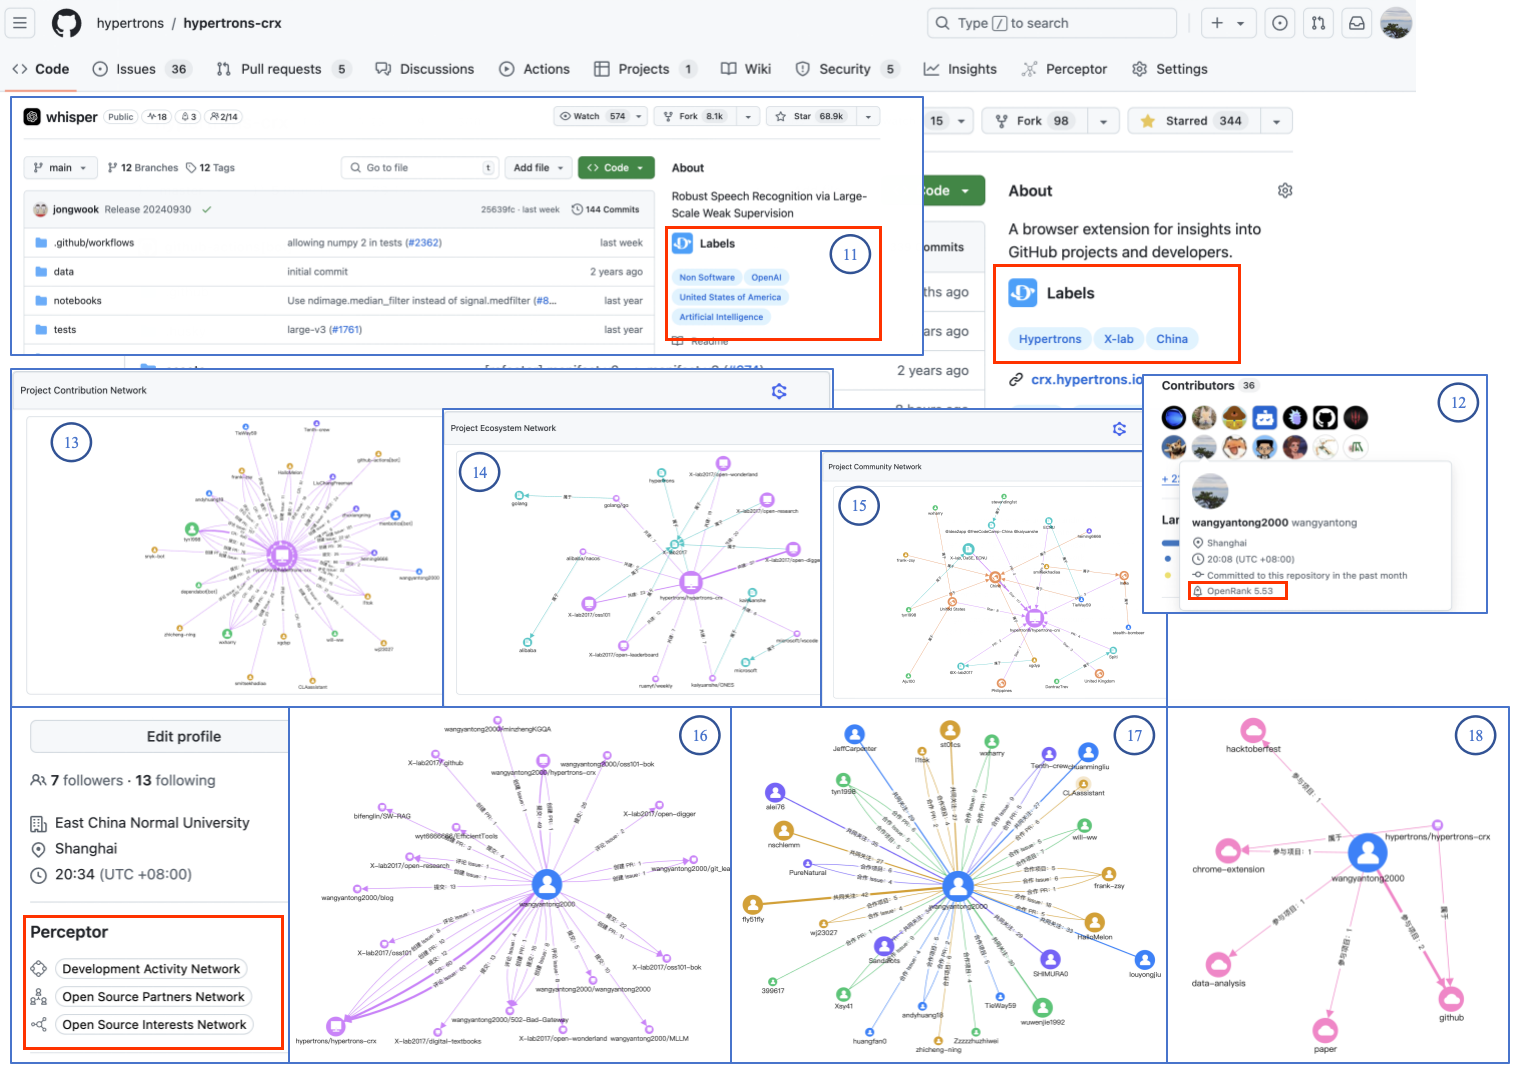
\includegraphics[width=\linewidth]{figures/chapter11/originals/hypercrx2-6.png}
\caption{Contextual and relational views in HyperCRX~2.0. Reproduced from Figure~2 of \citet{wang2025hyper}, using the image embedded in the author-supplied paper. Original callouts are retained: 11--12 identify labels and contributor information; 13--18 identify the six graph views described in the text. The figure documents the paper's interface version.}
\label{fig:ch11-hypercrx}
\end{figure}

The extension also incorporates language-model assistance for documentation and project analysis. In this chapter, that feature is relevant as an interface facility: a generated explanation should remain connected to the records and calculations it describes. It supplies no additional evidence that a collaboration score is valid, and the tool paper does not establish a controlled improvement in judgment quality. The disciplinary contribution of the extension is the integration of analytical access with an existing workflow; stronger claims about user outcomes require a separate study.

A useful evaluation task would ask maintainers to identify the cause of an apparent change in contribution. Completion time alone would be insufficient. The study would also need to examine whether the participant selected the correct time window, recognized a change in coverage, and distinguished an account's observed activity from the quality of its work. Such a task evaluates the reasoning supported by the interface, rather than the number of features it exposes.

\subsection{OSGraph and OpenGalaxy: two forms of relational inquiry}
OSGraph provides a graph-oriented environment for querying and inspecting open source communities \citep{huang2024}. The supplied paper describes a data pipeline involving OpenDigger, analytical storage, graph storage, and visual analysis. Its interface combines a graph canvas, search, an overview panel, analysis controls, view controls, and a timeline. Node expansion, common connections, paths, and community detection make relationships available for focused investigation.

\begin{figure}[htbp]
\centering
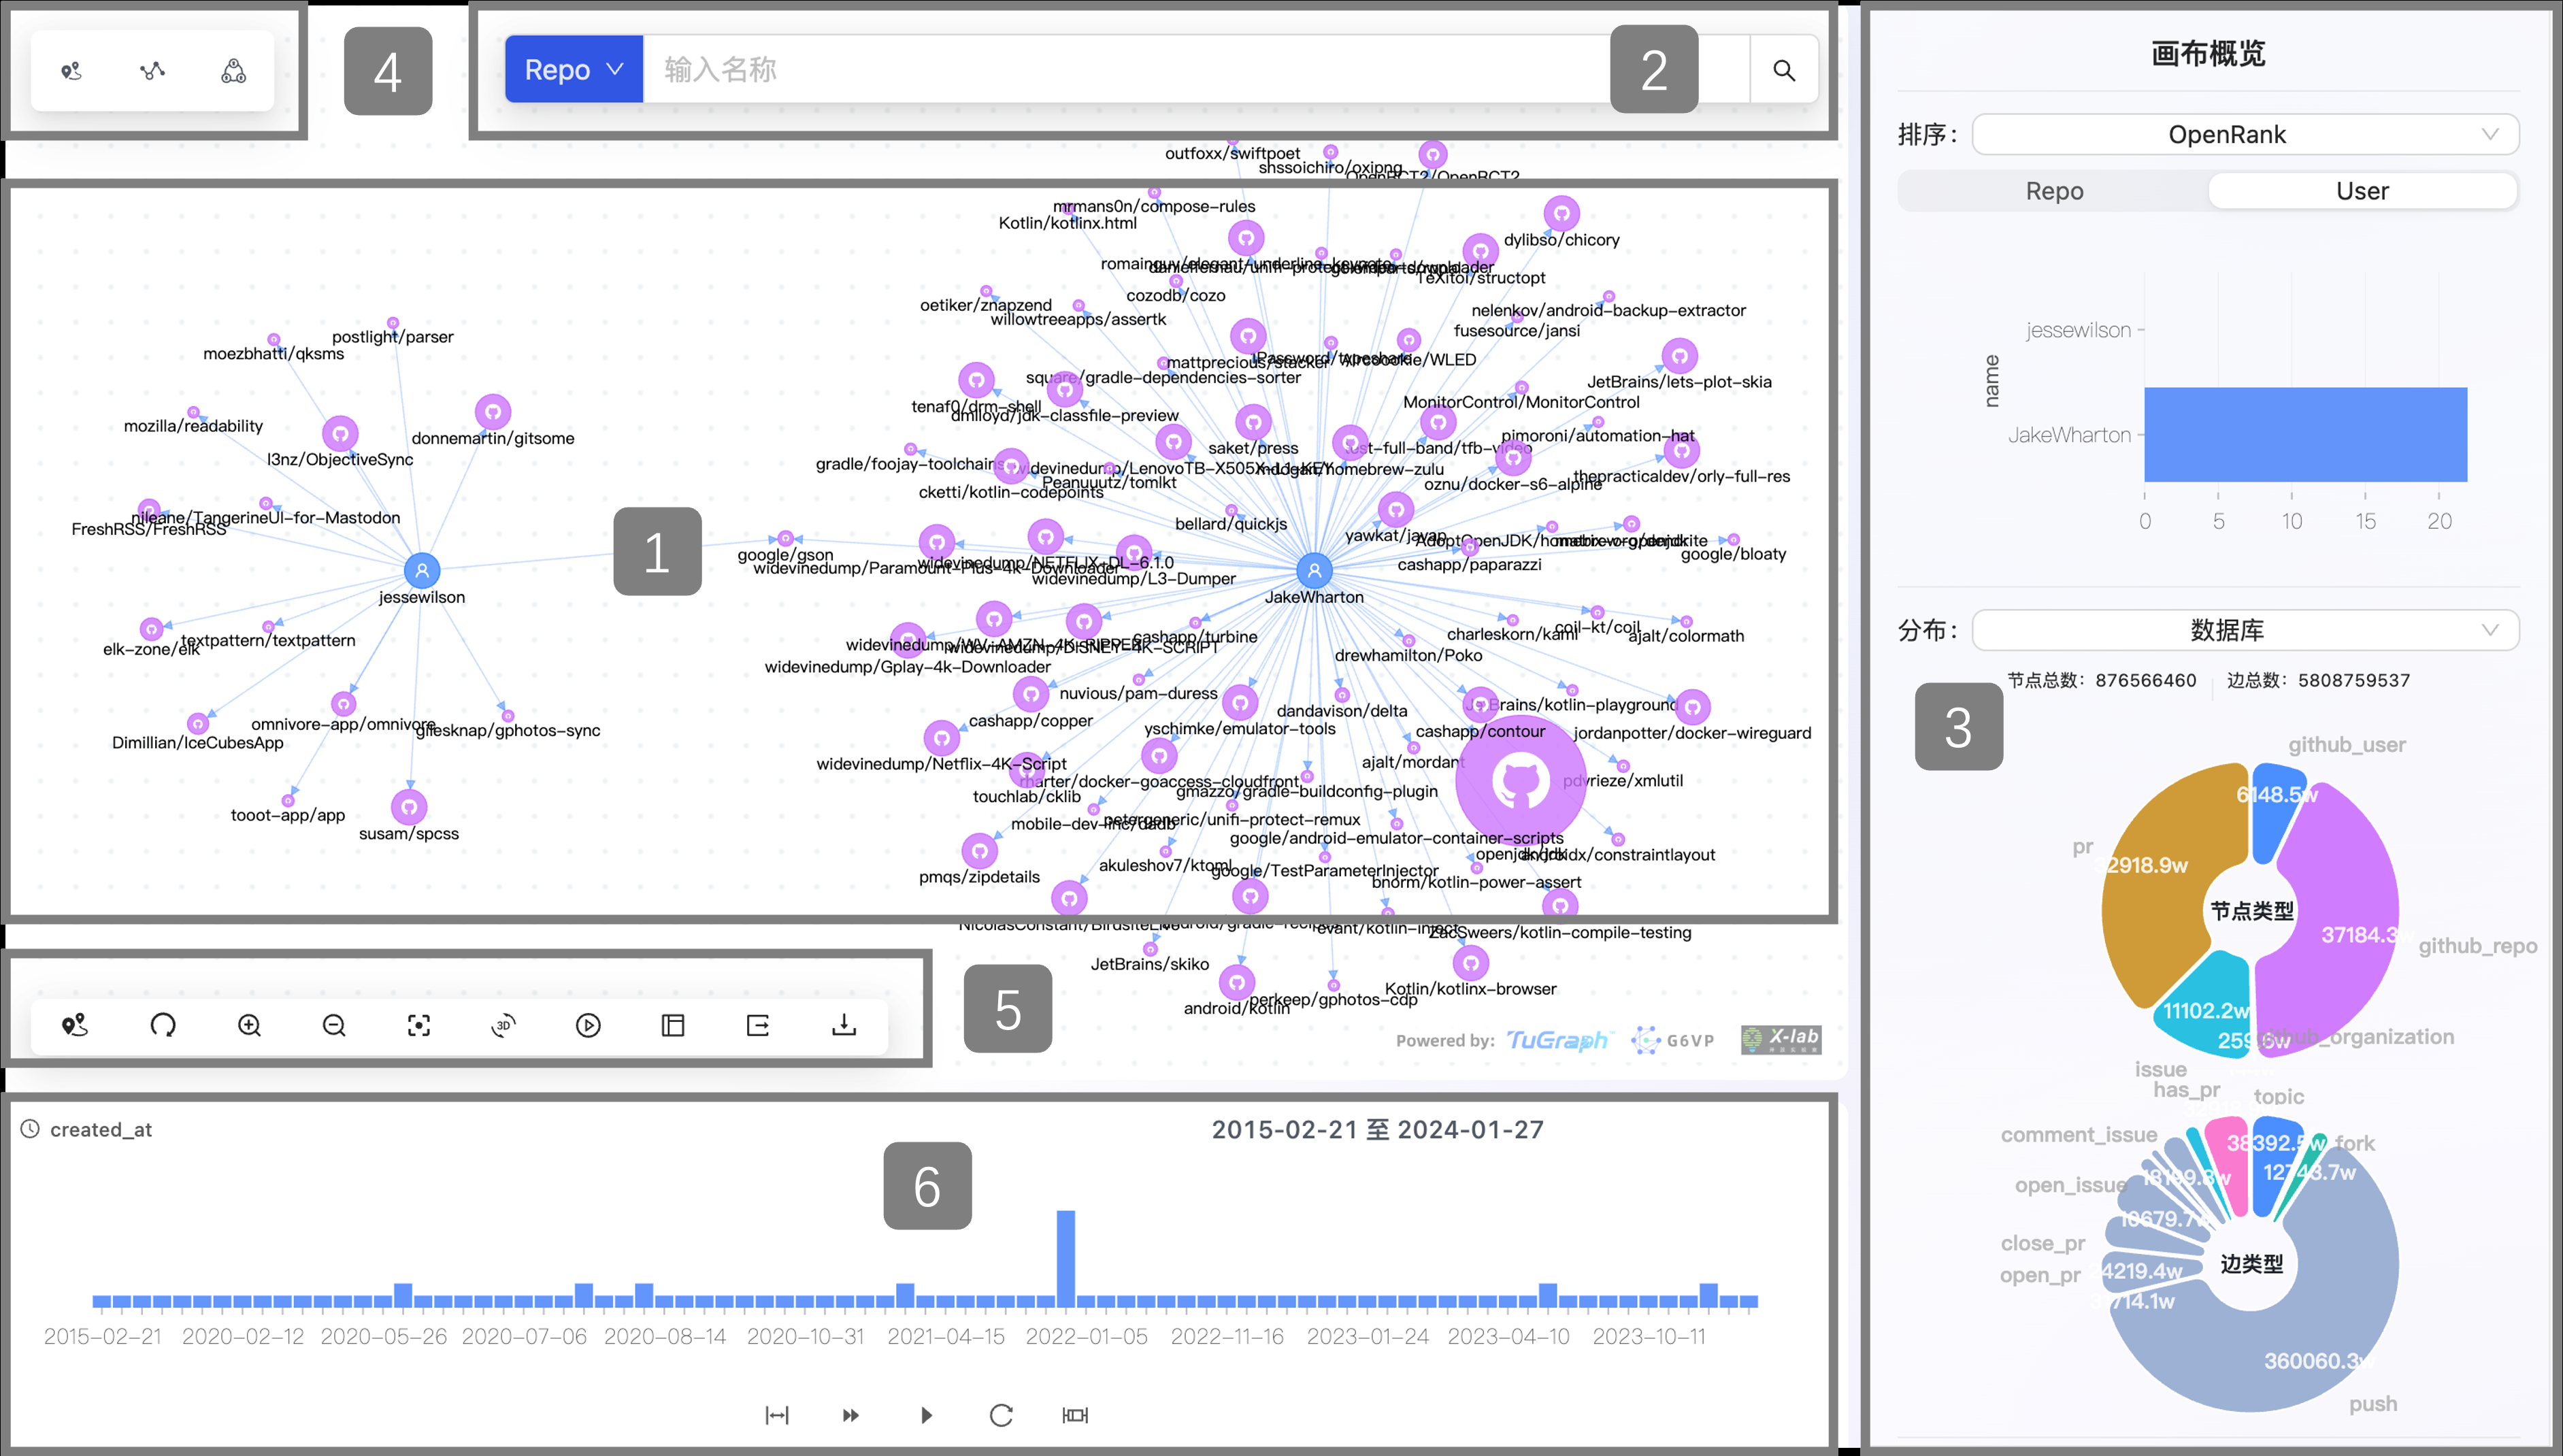
\includegraphics[width=\linewidth]{figures/chapter11/originals/osgraph-18.png}\par\vspace{5mm}
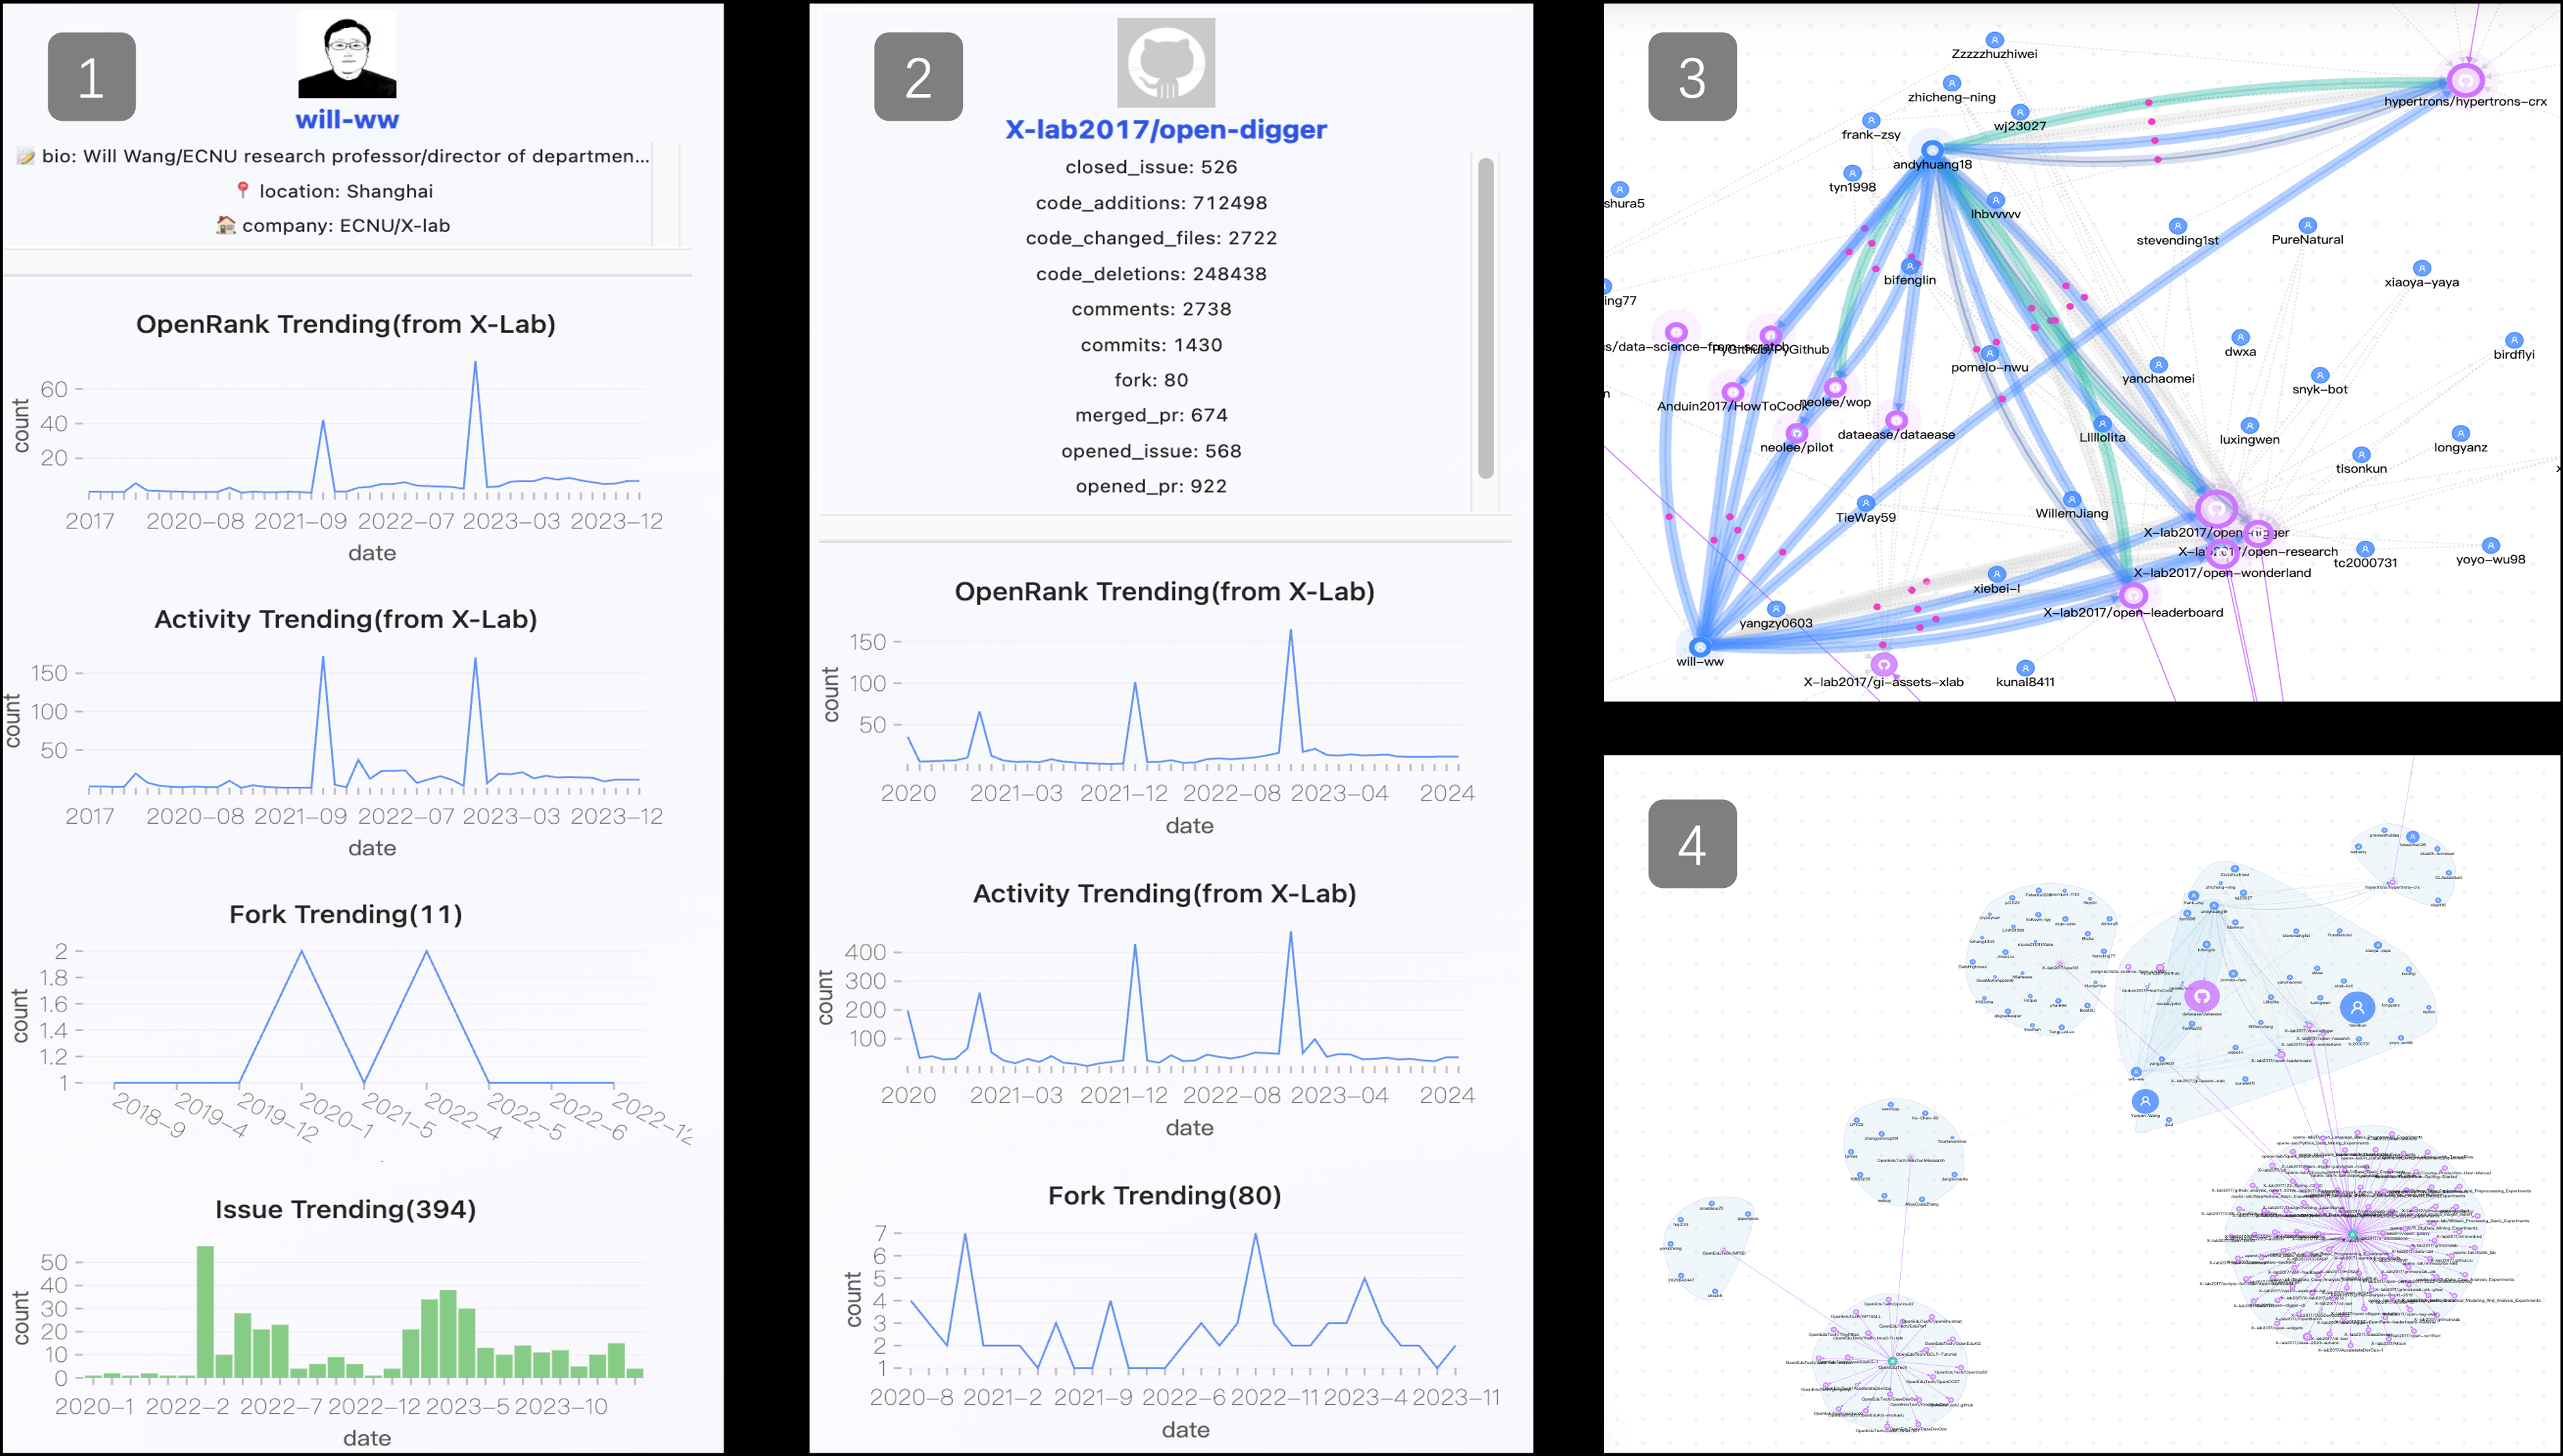
\includegraphics[width=\linewidth]{figures/chapter11/originals/osgraph-19.png}
\caption{OSGraph's analytical workspace and entity inspection. Top: the six interface regions in the paper's Figure~3. Bottom: the developer, repository, and relational examples in its Figure~4. Both images are reproduced at their embedded resolution from \citet{huang2024}; original labels and historical values are retained. Paths and detected communities describe the selected graph, rather than independently verified organizational relationships.}
\label{fig:ch11-osgraph}
\end{figure}

Figure~\ref{fig:ch11-osgraph} connects the history of an entity with its surrounding network. The combination is useful when an aggregate conceals a change in composition. An analyst may inspect whether a project's activity depends on a small set of collaborators, then examine those collaborators' other recorded relationships. The inference remains conditional on the graph. A path indicates a connection through the included relation types; it does not by itself demonstrate dependency, command, or knowledge transfer.

OpenGalaxy addresses a different scale of exploration \citep{zhang2024galaxy}. The 2024 research platform constructs a collaboration network from developer--repository participation, computes a repository projection, and presents a navigable three-dimensional view. Its paper distinguishes blue repository nodes from yellow developer nodes and uses different quantities for their sizes. The interface supports searching, navigation, neighbouring entities, and historical activity information. Figure~\ref{fig:ch11-galaxy} preserves this original representation.

\begin{figure}[htbp]
\centering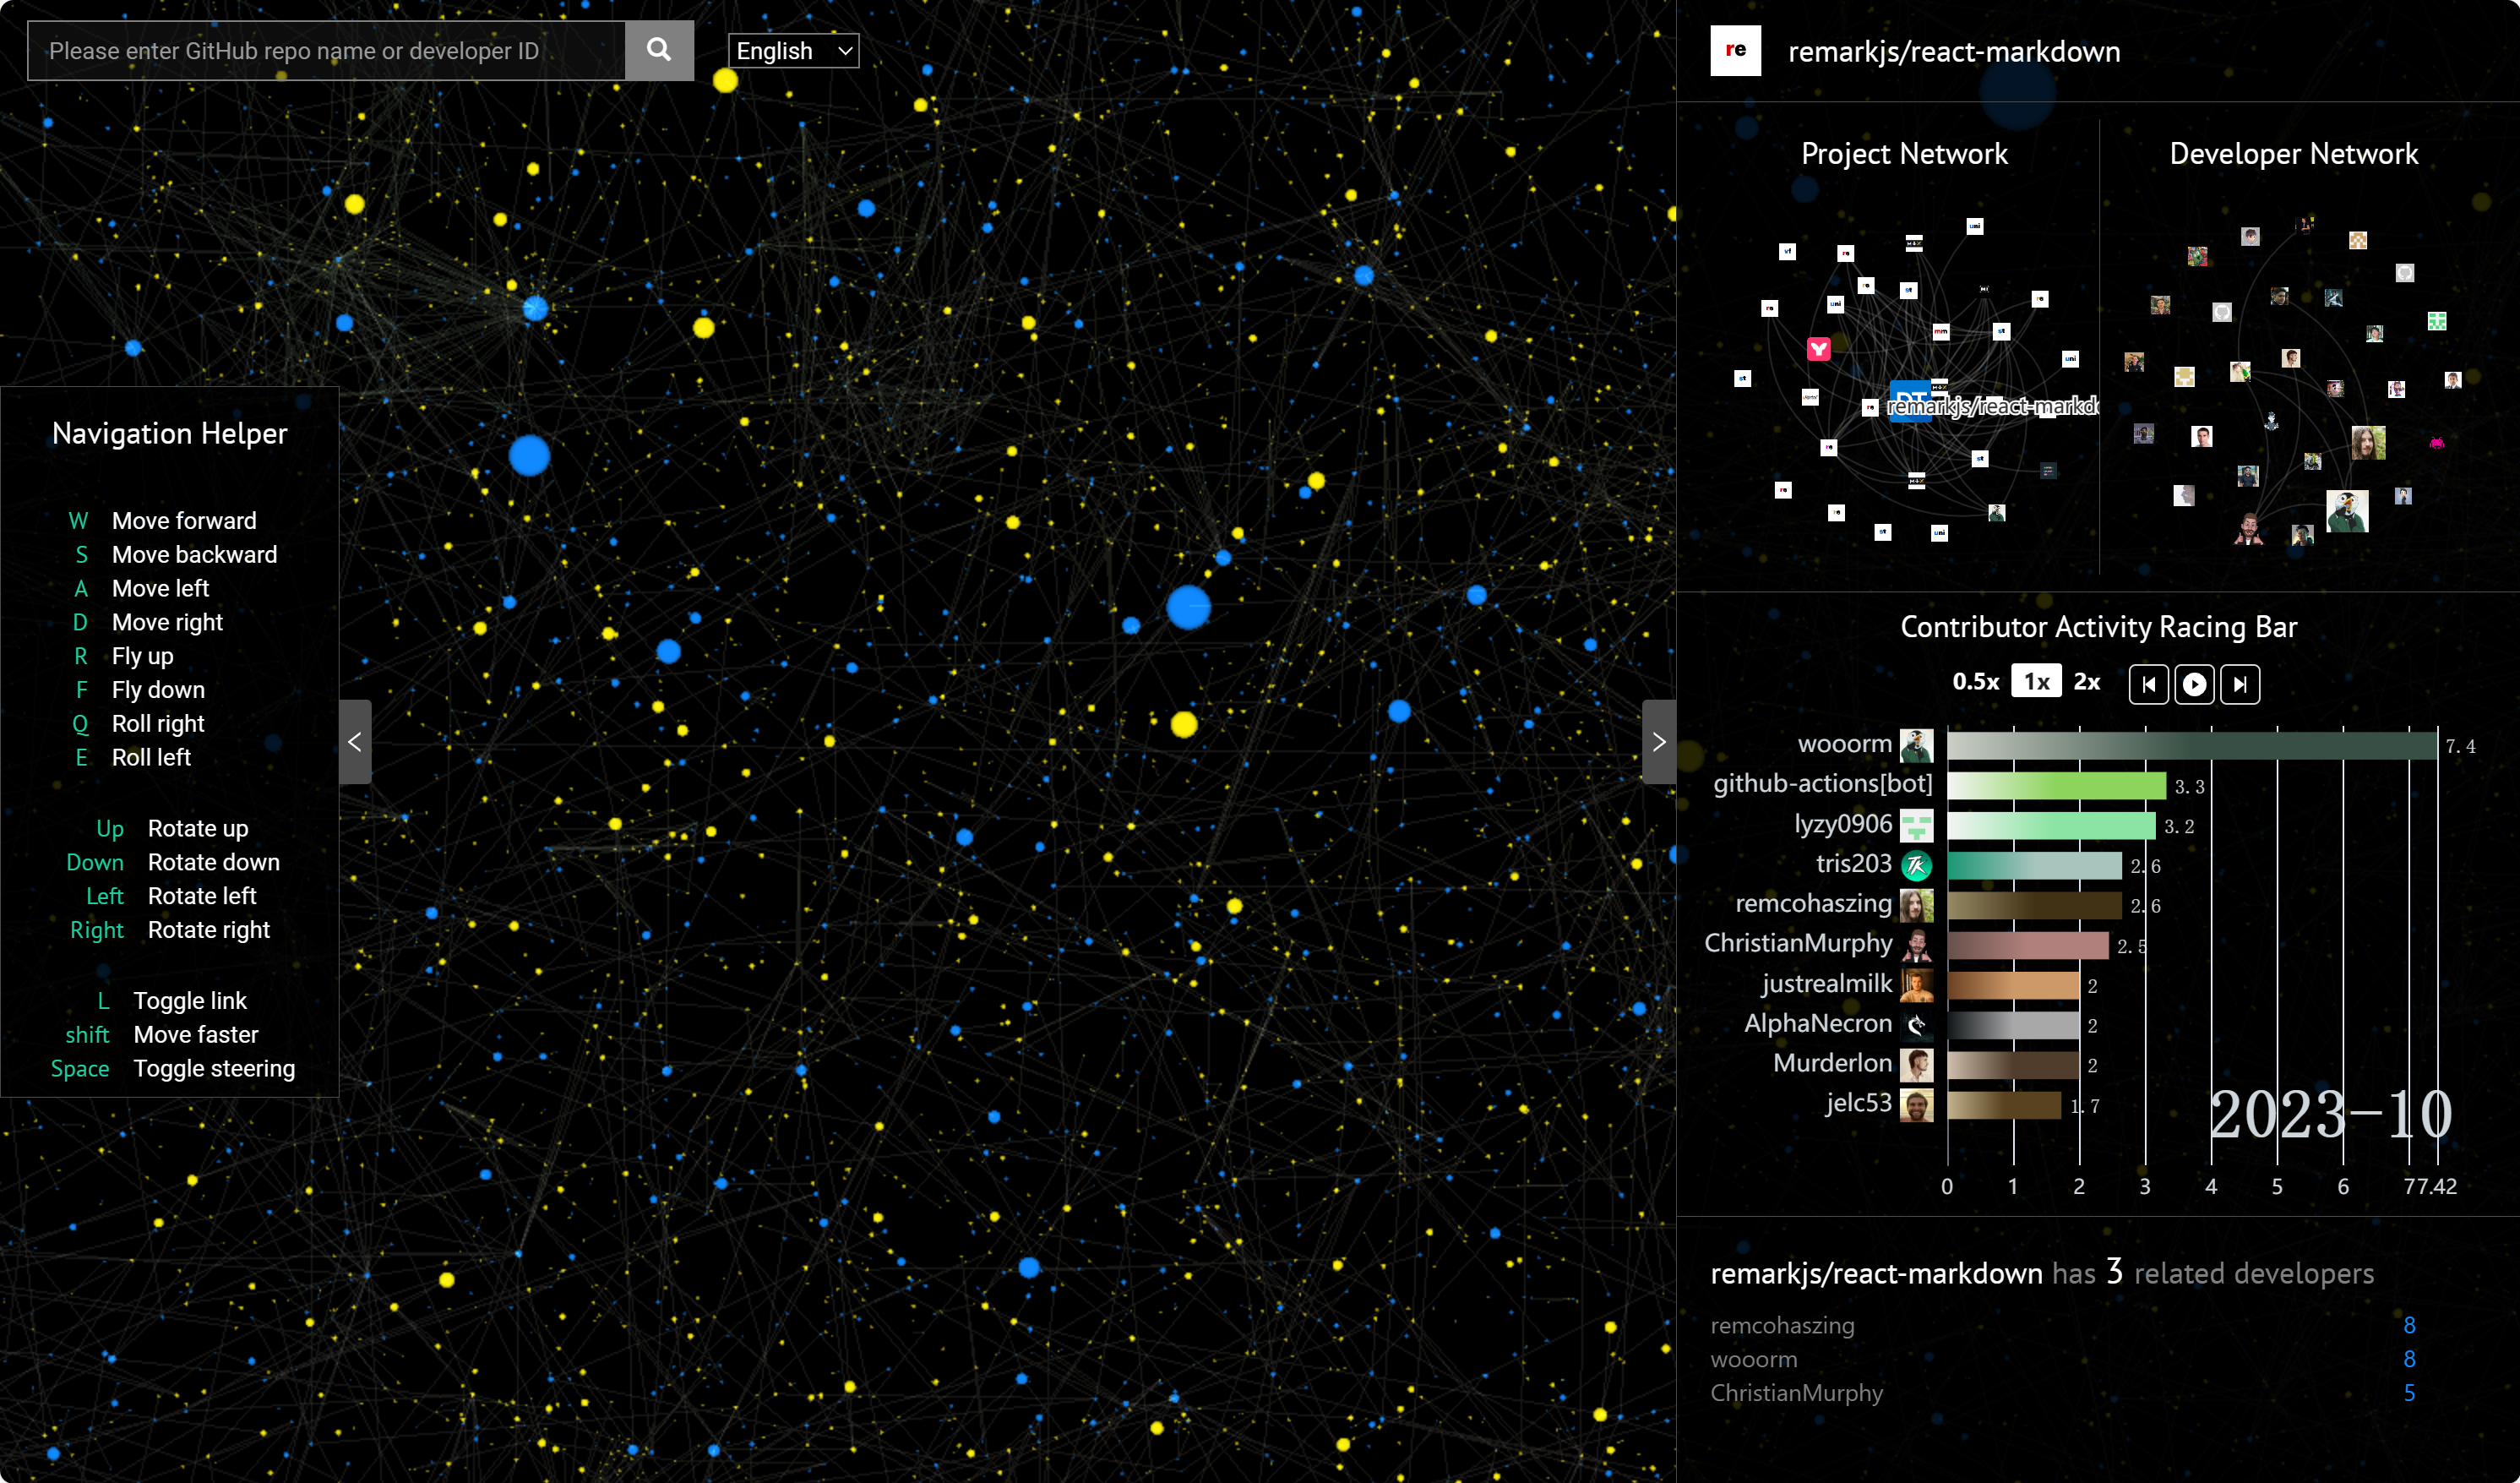
\includegraphics[width=\linewidth]{figures/chapter11/originals/opengalaxy-41.png}
\caption{The OpenGalaxy research platform described in 2024. Reproduced from Figure~2 of \citet{zhang2024galaxy}. The overview, navigation controls, selected entity, and neighbouring networks connect global exploration with local inspection. This historical platform and its graph construction are distinguished from the Open Galaxy module of OpenDipper discussed in Chapter~10.}
\label{fig:ch11-galaxy}
\end{figure}

In the historical repository projection, a developer's participation in two repositories contributes to their connection through
\[
 w_{ab}=\sum_{d\in D_a\cap D_b}
 \frac{A_{da}A_{db}}{A_{da}+A_{db}},
\]
where the activity quantities follow that paper's specification. The formula is retained here to expose the meaning of a displayed edge. It expresses a relation through shared participation. It is not a software-dependency relation, and it should not be silently relabelled as one. The repository projection and weighted PageRank described in the 2024 implementation also remain distinct from the later heterogeneous OpenRank formulation developed in Chapter~5.

These two explorers complement each other at the level of inquiry. An overview can suggest a region of the collaboration network to investigate. A query-oriented workspace can then make selected relations explicit. Neither a visually separated cluster nor a prominent node constitutes an explanation on its own. Layout thresholds, force calculations, and the included population affect what is visible. The scientific record must preserve those choices as well as the image.

Visualization research provides a concise discipline for assessing such interfaces. \citet{munzner2009} distinguishes domain problems, data and task abstractions, visual encodings and interactions, and implementation algorithms. Success at one level does not repair an error at another. For our ecosystem, this implies separate questions about whether an explorer addresses a real analytical task, represents the appropriate relations, supports accurate interpretation, and computes responsively. The supplied tool papers establish implemented designs and demonstrations; they do not settle all four questions.

\subsection{OpenTalent: participation across educational boundaries}
OpenTalent makes the connection between educational participation and open source communities visible at an institutional scale. The supplied observatory screenshot records 6,521 participating students, 692 universities, 224 communities, and 2,312 projects, with an update date of December~2024 \citep{xlab2024talent}. Figure~\ref{fig:ch11-talent} reproduces this snapshot without changing its values. These are the dashboard's displayed coverage counts, not a census of all university participation and not measures of learning effectiveness.

\begin{figure}[htbp]
\centering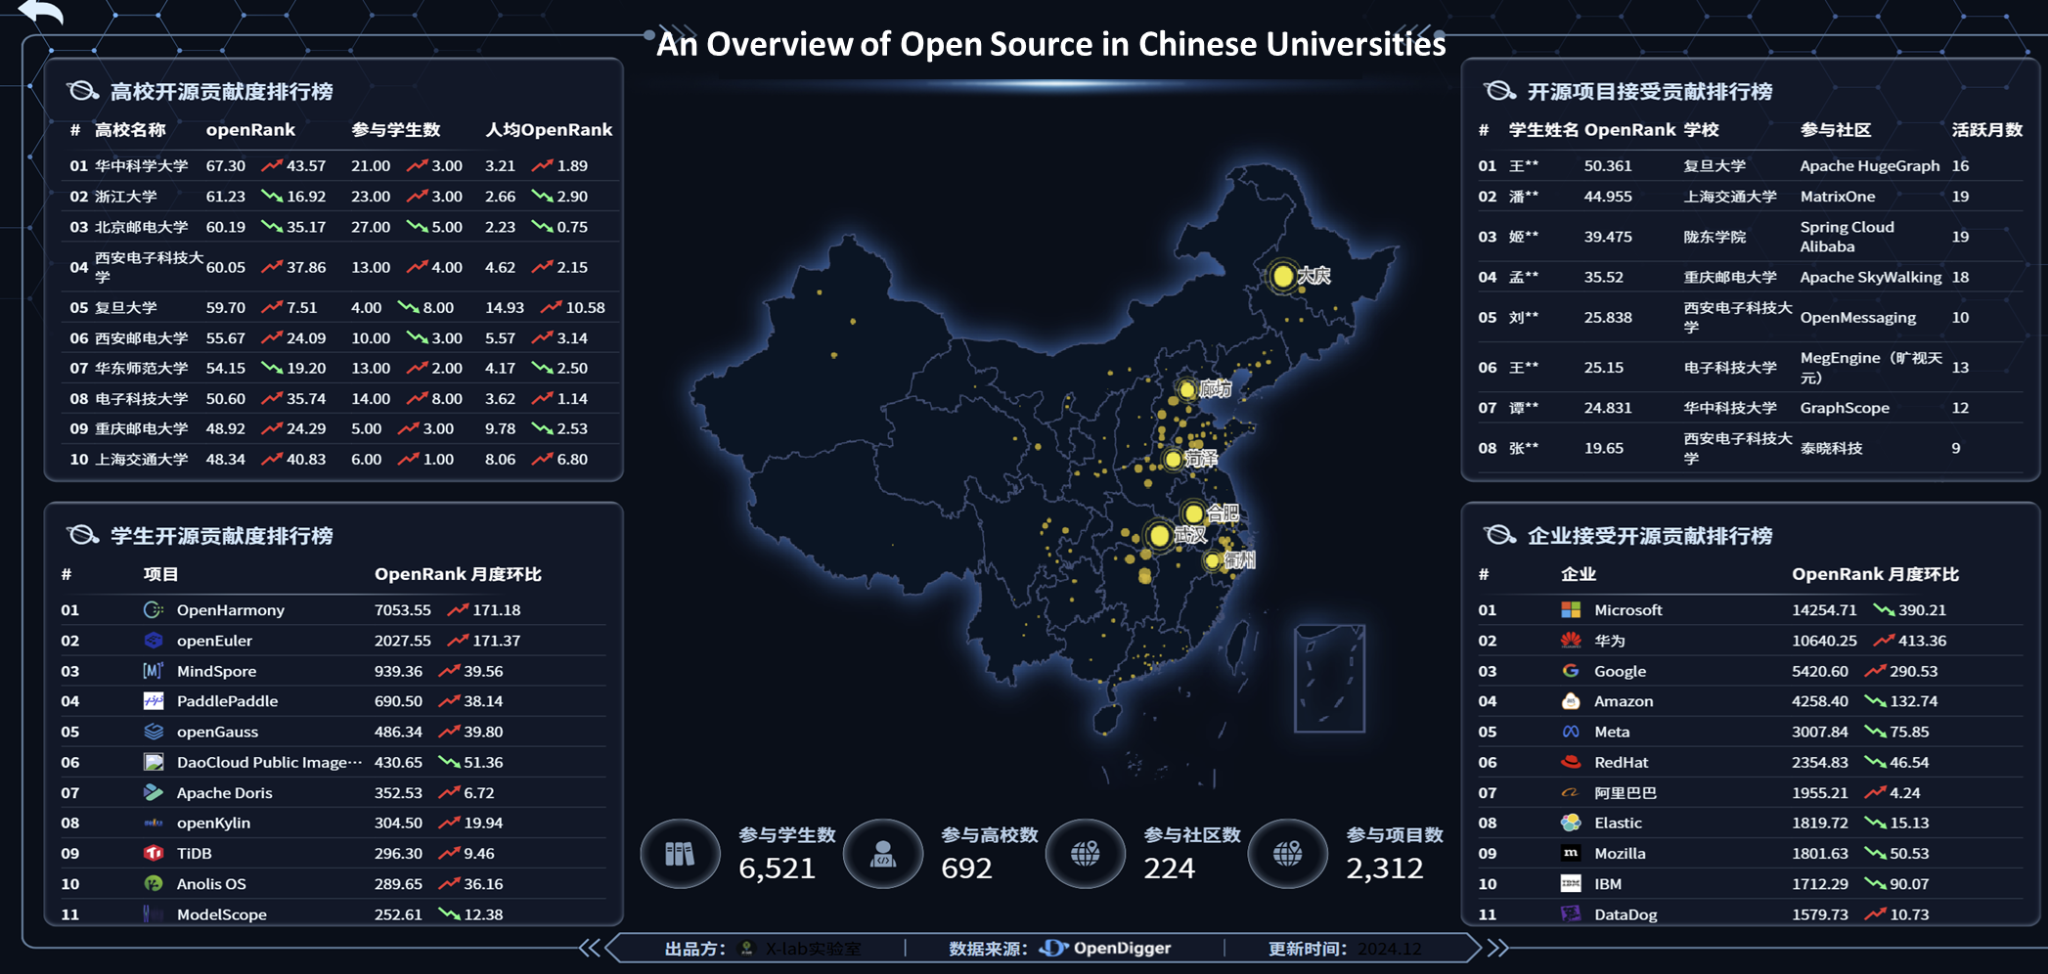
\includegraphics[width=\linewidth]{figures/chapter11/originals/opentalent-2024-12.png}
\par\vspace{4mm}
{\sffamily\color{HeadingInk}\small
\begin{tabularx}{\linewidth}{@{}*{4}{>{\centering\arraybackslash}X}@{}}
\textbf{6,521} & \textbf{692} & \textbf{224} & \textbf{2,312}\\
Students & Universities & Communities & Projects
\end{tabularx}}

\caption{OpenTalent's university participation observatory, supplied by the authors \citep{xlab2024talent}. The December~2024 snapshot reports 6,521 students, 692 universities, 224 communities, and 2,312 projects. The original Chinese interface and masked student names are preserved. Its panels juxtapose institutional participation, projects, individual records, and companies; the displayed rankings do not establish learning outcomes or institutional educational quality.}
\label{fig:ch11-talent}
\end{figure}

The observatory extends the course-level cases of Chapter~7. A course assessment concerns particular learning objectives and participants under known teaching conditions. An institutional observatory concerns participation across many settings, with much weaker control over entry conditions, opportunities, and attribution. Its value is to locate relationships that warrant investigation: which communities receive student contributions, how participation persists beyond a course, and where students encounter opportunities for collaborative work.

An appropriate investigation would link the observable participation record to a portfolio of work and its educational context. The record can identify a contribution and its discussion; an assessor can examine the technical and collaborative work involved; the student can explain decisions and reflect on feedback. These sources answer different questions. A university total cannot substitute for an individual learning assessment, and a student's network position cannot by itself establish a transferable competence.

The OpenTalent example clarifies why an ecosystem needs several interfaces. A national overview locates patterns, a project view explains the setting of a contribution, and a portfolio supports assessment of the work. The handover should preserve identity, date, and provenance. This is also the requirement encountered in OpenDipper, but the immediate task is different: educational interpretation here, and institutional investigation in Chapter~\bookref{ch:thinktanks}{10}. The common requirement can be studied across tools without treating their purposes or outcomes as interchangeable.

\FloatBarrier
\section{Validation and Shared Benchmarks}
\label{sec:ch11-benchmarks}

\subsection{OpenPerf and common reference conditions}
OpenPerf addresses a recurring difficulty in open source research: abundant observations do not by themselves create a common basis for comparison \citep{han2025openperf}. Its three benchmark categories connect methodological testing to practical evaluation. Task benchmarks compare methods on specified problems. Index benchmarks supply defined representations of an entity or arrangement. Exemplar benchmarks identify a selected practice or performance level as a reference. A strong result in one category does not automatically validate the next.

The published framework specifies six elements of a task benchmark: its name, open source scenario, task type, dataset, models, and evaluation criteria. Table~\ref{tab:ch11-tasks} condenses the nine task definitions in the paper. Their diversity matters. Completion, classification, ranking, anomaly detection, and recommendation require different targets and reference evidence. Their results cannot be combined into one undifferentiated measure of ecosystem quality.

\begin{table}[htbp]
\caption{The nine task benchmarks defined in OpenPerf. Condensed and translated from Tables 1--2 of \citet{han2025openperf}. Only three tasks receive comparative experimental results in that paper.}
\label{tab:ch11-tasks}
\centering\small\renewcommand{\arraystretch}{1.17}
\begin{tabularx}{\linewidth}{@{}>{\raggedright\arraybackslash}p{.33\linewidth}>{\raggedright\arraybackslash}X>{\raggedright\arraybackslash}X@{}}
\toprule
\textbf{Task} & \textbf{Target or reference} & \textbf{Evaluation in the source}\\\midrule
Behaviour completion and prediction & Behaviour series from five projects; observations removed to form a completion problem. & NMSE, NRMSE, NMAE; comparative experiment.\\[5pt]
Bot identification and classification & Account features with labels assembled using existing detectors and manual work. & Classification measures; comparative experiment.\\[5pt]
Comment sentiment classification & Positive and negative issue comments; manually assigned labels. & F1 and precision specified.\\[5pt]
Software supply-chain risk prediction & Project attributes used to construct a maintainability assessment. & No task evaluation measure specified in source Table 2.\\[5pt]
Project influence ranking & A repository collaboration graph and influence-ranking procedure. & Algorithm runtime specified.\\[5pt]
Archived-project prediction & Repository features and archive status from GitHub. & F1 and precision specified.\\[5pt]
Network influence-index prediction & Project metrics used to predict an influence value. & MSE and RMSE specified.\\[5pt]
Community anomaly detection & Behaviour series; labels informed by clustering and expert judgment. & F1 and precision specified.\\[5pt]
Project recommendation by link prediction & Graphs based on shared participation, shared topics, and their combination. & AUC and runtime; comparative experiment.\\
\bottomrule
\end{tabularx}
\tablenote{The descriptions retain the roles of the source tasks. Recovery of removed observations or links does not, without a temporal protocol, establish performance on future events. A model-generated index is also distinct from an independently observed outcome.}
\end{table}


The framework is also an example of practice informing research design. Enterprise governance, software development, community operations, and ecosystem strategy generate different demands on the same underlying data. A missing-data problem encountered in a dashboard becomes a completion task; uncertainty about automated participation becomes a classification task; finding potentially relevant projects becomes a link-prediction task. The problem is abstracted sufficiently for method comparison while retaining the application that gives the comparison meaning.

\subsection{Three experiments and their evidential scope}
The OpenPerf paper reports experiments for three representative tasks. Table~\ref{tab:ch11-results} reproduces selected results from its completion and bot-classification experiments; Figure~\ref{fig:ch11-link} redraws the full reported link-prediction comparison. These are historical results from the published study. They are not new executions of the algorithms or a comparison with subsequent releases.

\begin{table}[htbp]
\caption{Selected OpenPerf results for two representative tasks. Values are transcribed from Tables 3--4 of \citet{han2025openperf}. Bold entries identify the best value within the corresponding published comparison.}
\label{tab:ch11-results}
\centering\small\renewcommand{\arraystretch}{1.17}
\begin{tabularx}{\linewidth}{@{}Xrrl@{}}
\toprule
\multicolumn{4}{@{}l}{\textbf{(a) Behaviour completion: NMSE, lower is better}}\\[3pt]
\textbf{Project} & \textbf{TAMF} & \textbf{Best alternative} & \textbf{Alternative method}\\\midrule
PyTorch & \textbf{0.041} & 0.161 & iForest\\
SkyWalking & 0.235 & \textbf{0.143} & iForest\\
TensorFlow & \textbf{0.024} & 0.031 & TRMF\\
TiDB & \textbf{0.043} & 0.124 & TRMF\\
VS Code & \textbf{0.234} & 0.326 & TRMF\\
\bottomrule
\end{tabularx}
\vspace{6mm}
\begin{tabularx}{\linewidth}{@{}Xrrr@{}}
\toprule
\multicolumn{4}{@{}l}{\textbf{(b) Bot classification: higher is better}}\\[3pt]
\textbf{Method} & \textbf{Accuracy} & \textbf{F1} & \textbf{AUC}\\\midrule
Logistic regression & 0.9234 & 0.4856 & 0.5760\\
Decision tree & 0.7995 & 0.3408 & 0.5024\\
SVM & 0.8936 & 0.4609 & 0.5414\\
Gaussian naive Bayes & \textbf{0.9548} & 0.5923 & 0.5319\\
$K$-nearest neighbours & 0.8309 & 0.3706 & 0.5119\\
Random forest & 0.8817 & 0.4880 & 0.6486\\
BotHunter & 0.8649 & 0.3405 & 0.5512\\
BoDeGHa & 0.8286 & 0.3628 & 0.5049\\
BotHawk & 0.8799 & \textbf{0.8821} & \textbf{0.9472}\\
\bottomrule
\end{tabularx}
\tablenote{Panel (a) selects NMSE from the three reported error measures and retains TAMF plus the best of the seven alternatives for each project. Panel (b) retains all nine methods and three of the five reported measures. Original values are preserved; confusion matrices, uncertainty intervals, and new replications are not supplied here.}
\end{table}


The completion experiment uses behaviour series from five active projects during 2020 and introduces missing observations. In the reported NMSE comparison, TAMF gives the lowest value for PyTorch, TensorFlow, TiDB, and VS~Code, while iForest gives the lowest value for SkyWalking. The exception is informative: a method designed to exploit temporal structure does not lead on every series. The paper connects this difference to weaker periodicity in SkyWalking. For deployment, an additional question is whether the experimental missingness resembles the actual collection failure. Randomly removed observations and a prolonged service outage can require different tests.

The bot-classification experiment compares nine methods on a constructed account dataset. BotHawk has the highest reported F1 and AUC, whereas Gaussian naive Bayes has the highest reported accuracy. The values in Table~\ref{tab:ch11-results} retain that distinction. The result supports a comparison under the study's labels and protocol; it does not establish that one model will remain best across changing bot populations. A new application should specify which classification errors matter, disclose the account selection and labelling process, and evaluate transfer to the intended population.

The link-prediction experiment constructs three repository graphs: shared developer participation, shared topic labels, and their combination. The dataset definitions therefore vary the meaning of a relation as well as the representation. The reported comparison shows strong performance for methods based on local graph information. WICRA has the highest AUC in each of the three graphs, while RA runs faster. On the shared-participation graph, their reported pairs are 0.9759 and 2,561.7305 seconds for WICRA, and 0.9676 and 394.6628 seconds for RA. These observations expose an accuracy--runtime trade-off within the original experiment.

\begin{figure}[htbp]
\centering\includegraphics[width=\linewidth]{figures/chapter11/fig11-07-openperf.pdf}
\caption{OpenPerf's published link-prediction comparison, redrawn from Table~5 of \citet{han2025openperf}. Top: AUC, with a deliberately restricted horizontal range to show differences. Bottom: reported runtime in seconds on a logarithmic scale. All eight methods and all three graph datasets are retained. Runtime comparisons apply to the original execution conditions; the study reports no uncertainty intervals for these entries.}
\label{fig:ch11-link}
\end{figure}

Random removal of observed links tests recovery under the chosen removal mechanism. It is not equivalent to predicting future participation from information available at an earlier date. Nor does a high AUC establish that a recommendation helps a newcomer find a suitable project. That latter claim requires observation of use, including relevance, access to assistance, and the experience of attempting a contribution. The benchmark makes an algorithmic claim examinable; further evidence connects it to a practical one.

\subsection{Validation across levels}
The chapter's synthesis separates five responsibilities. \emph{Measurement validation} examines whether the observations and representation support the intended interpretation. \emph{Computational validation} checks whether the implementation realizes the specified procedure. \emph{Task validation} compares performance against an independently specified target and protocol. \emph{Use validation} examines whether people can interpret and apply the result appropriately. \emph{Consequential evaluation} examines what changes when the evaluation is deployed. These responsibilities interact, but evidence for one does not discharge the others.

The cases locate these responsibilities precisely. Activity requires an account of the work represented by its selected events; OpenRank requires both a specified computation and a justified interpretation of the graph. OpenPerf tests performance on a defined task, while OpenTalent's educational use requires evidence about learning. For a think-tank product, Table~\bookref{tab:ch10-use}{10.3} separates implementation and dissemination from institutional uptake and consequences. Its application-specific distinctions become part of this wider validation practice. The five responsibilities synthesize these requirements; they do not replace the evaluation-system components in Chapter~3.

Common benchmarks should therefore preserve the target, population, time separation, labels, and selection procedure alongside the score. A temporal task should distinguish data available at the forecast date from later information. A transfer task should identify the communities withheld from development. A computational comparison should state the graph, configuration, hardware, and stopping rule. These obligations implement the evaluation design developed in Chapter~3 at the scale of shared research practice.

The benchmark itself must be open to revision. A task can become easier because its labels are predictable from an unintended feature; a popular dataset can become unrepresentative of new communities; a frequently inspected test set can cease to provide an independent comparison. Retaining a stable historical release supports replication, while publishing a documented successor supports progress. A field needs both continuity of reference and the ability to question what the reference represents.

\FloatBarrier
\section{Interdisciplinary Foundations}
\label{sec:ch11-interdisciplinary}

The interdisciplinary basis of Open Source Evaluatology is methodological as well as substantive. It draws on neighbouring fields to answer different parts of an evaluation question. The purpose is to connect these contributions around open collaboration, while preserving the assumptions that make each one useful. Table~\ref{tab:ch11-bridges} summarizes the resulting research connections.

\begin{table}[htbp]
\caption{Interdisciplinary connections as a research design. The right-hand column states research directions proposed in this chapter, rather than completed experiments.}
\label{tab:ch11-bridges}
\centering\small\renewcommand{\arraystretch}{1.17}
\begin{tabularx}{\linewidth}{@{}>{\raggedright\arraybackslash}p{.24\linewidth}>{\raggedright\arraybackslash}X>{\raggedright\arraybackslash}X@{}}
\toprule
\textbf{Connection} & \textbf{Contribution to open source evaluation} & \textbf{Reciprocal research opportunity}\\\midrule
Measurement theory & Distinguish an index, an attribute, its interpretation, and the consequences of use. & Study interpretation and measurement change when a public score becomes an incentive.\\[6pt]
Network science & Match relations and centrality to the process being represented; distinguish position from causal influence. & Compare graph constructions against documented episodes of open collaboration.\\[6pt]
Software engineering and visual analytics & Connect events with work practices; validate domain tasks, representations, interfaces, and algorithms separately. & Assess whether tools help users reconstruct and correctly interpret evaluation evidence.\\[6pt]
Education and learning analytics & Relate participation to learning objectives, work samples, feedback, and opportunities to learn. & Follow transitions from course participation to sustained community contribution.\\[6pt]
Institutional research and science policy & Explain resource conditions, collective action, and the behavioural effects of public evaluation. & Examine how recognition and decision-support arrangements alter collaboration and maintenance.\\
\bottomrule
\end{tabularx}
\tablenote{The connections draw on the primary literature discussed in Section~11.5. They preserve differences among theoretical positions and avoid treating a borrowed concept as independent evidence for a claim about open source.}
\end{table}


\subsection{Measurement theory and valid interpretation}
Measurement theory makes the distinction between a reproducible number and an adequately supported interpretation explicit. \citet{messick1995} places interpretations and their implications for use within a unified account of validity. \citet{borsboom2004}, by contrast, argues for a causal conception: the attribute being measured must exist and produce variation in the measurement outcomes. These positions should not be presented as a single settled doctrine. Their disagreement exposes two questions relevant to our field: what generates a score, and what warrants the meaning and use assigned to it?

For open source evaluation, the distinction is particularly important because some quantities are deliberately constructed indices. Activity combines selected behaviours according to a rule. It need not be understood as a reflective test of a hidden psychological trait. A claim that it represents a useful dimension of participation requires a defence of its selected events, weights, aggregation, and setting. A claim that it measures competence requires additional evidence about competence. The latter does not follow from the former, even if both quantities correlate in a particular sample.

Software measurement supplies a closely related tradition. \citet{kitchenham1995} connects entities, attributes, instruments, units, and validation within a measurement framework. The practical implication for our work is to document the complete measurement operation. A change in repository scope or identity resolution can change a result even when its algebra remains unchanged. The versioned specifications developed in Chapters~4--6 are a response to this problem.

Open source collaboration contributes a useful setting for extending these debates. Its measurements are often public, recurrent, and used by the people whose behaviour generates them. A research programme can examine how the validity of an interpretation changes after a measure becomes part of a recognition or governance process. The resulting evidence can refine both the construct and the conditions under which it is useful.

\subsection{Network science, software engineering, and relation semantics}
Network science supplies methods for studying interdependence, but a graph does not acquire an interpretation from topology alone. \citet{borgatti2005} shows that centrality measures imply different assumptions about the processes moving through a network. This matters for OpenRank and the graph tools: a relation through shared participation, a direct interaction, and a package dependency need not support the same interpretation of influence.

The distinction also separates relational prominence from a causal effect on others. Research on diffusion shows why correlated behaviour among connected actors can reflect selection into similar relationships as well as influence \citep{aral2009}. Open source examples add shared employers, common technical dependencies, and coordinated release schedules as plausible alternative explanations. A collaboration score can describe a position without resolving these explanations. Testing a diffusion claim requires a design appropriate to that claim.

Software engineering grounds the relations in work practices. Issue discussion, review, integration, maintenance, and release management have different roles in producing and sustaining software. Their traces should be interpreted with knowledge of those roles. Trace ethnography offers one way to combine documentary records with situated understanding of coordination \citep{geiger2011}. Applied to our setting, it can explain why an apparent burst of activity reflects a migration, why work is credited to a service account, or why a quiet maintainer remains essential.

The reciprocal contribution is a domain in which relational models can be examined against documented collaboration. Chapters~5 and~9 show how the definition of a relation and the boundaries of the object affect interpretation. Future studies can compare alternative graph constructions on the same underlying work episodes, asking which relationships preserve the mechanisms relevant to the evaluation question. Such comparisons would contribute more than another ranking correlation: they would explain when a particular network model is informative.

\subsection{Education, feedback, and learning}
Education provides an especially clear test of the field's ability to connect evidence with purpose. Situated learning treats participation in a community of practice as central to learning \citep{lave1991}. This perspective helps explain the interest in open source courses and OpenTalent, where students encounter existing practices and collaborators. It does not imply that a participation count is a direct measure of what a student has learned.

Learning analytics reinforces the need for theory in selecting and interpreting digital traces \citep{wise2015}. In an open source course, the same recorded action may have different meanings for a novice, an experienced contributor, and an instructor. A review comment may demonstrate a newly acquired skill, routine assistance, or a required exercise. Educational design and the learner's starting point help distinguish these interpretations.

Formative assessment adds the question of how evidence helps students act. \citet{nicol2006} emphasizes learners' active role in interpreting feedback and regulating their work. For OpenTalent, this suggests an interface that permits a student to inspect a contribution, connect it with a learning objective, and decide what to improve. A rank may draw attention; the educational value depends on the feedback process that follows.

The contribution of Open Source Evaluatology is to connect these processes to collaboration beyond the classroom. A prospective study could follow participation before, during, and after a course, combine work samples with independent assessment, and examine transitions into sustained community roles. The outcome would be a better-supported account of learning and participation, rather than a claim that one score measures both. It would also extend Chapter~7's evidence without treating the OpenTalent screenshot as a new educational experiment.

\subsection{Institutions, science policy, and evaluative consequences}
Institutional research explains why the conditions of collaboration belong inside the evaluation question. \citet{ostrom2009} provides a framework for organizing heterogeneous evidence about resource systems, users, governance, interactions, and outcomes. Its relevance here is the insistence on relationships and context. Software can be copied without exhausting the original artifact, whereas maintainer attention, review capacity, and organizational support remain limited. The analogy with natural-resource systems must therefore be adapted to the resources and practices at issue.

The theory of commons-based peer production gives open collaboration a more direct institutional interpretation. \citet{benkler2002} examines how distributed contributors coordinate information production through arrangements that differ from conventional markets and hierarchies. For evaluation, this directs attention to access, matching, integration, and the conditions under which contributions can be combined. It supports Chapter~2's concern with collective capability while leaving the value of a particular arrangement open to empirical examination.

Public evaluation then becomes part of the setting it describes. \citet{espeland2007} shows how rankings can change behaviour through commensuration and altered expectations. The application to open source is a research hypothesis, not an automatic prediction: recognition may make neglected work visible, but it may also redirect effort toward the recorded dimensions. Chapters~6 and~7 provide grounds for examining both possibilities. A suitable study observes the composition and quality of work as well as the reported score.

Science-policy research contributes principles for the responsible use of metrics. The Leiden Manifesto places quantitative information in relation to expert judgment and the purposes of assessment \citep{hicks2015}. In the think-tank setting of Chapter~10, this means that a regional or institutional comparison needs an explicit mission and interpretive process. The disciplinary contribution is to carry the same obligations through the underlying open source data, methods, and interfaces, so that scrutiny remains possible after the result enters a report.

These connections depend on common objects that different communities can use without agreeing on every purpose. \citet{star1989} describes boundary objects as sufficiently stable to support cooperation while remaining adaptable to different viewpoints. A versioned contribution record can serve such a role: a student, maintainer, teacher, and researcher can examine the same work while asking different questions. This is our proposed application of the concept. It explains why shared evidence need not require a single universal ranking or a single account of value.

\FloatBarrier
\section{Building a Cumulative Research Programme}
\label{sec:ch11-programme}

\subsection{Common practice without premature uniformity}
Cumulative inquiry depends on publishing the evaluation question together with the process that produces its evidence. Objects, scope, definitions, data releases, transformations, reference conditions, and intended use allow another researcher to examine the argument. A benchmark, a qualitative investigation, and an institutional evaluation need different records, but each should make its claims open to scrutiny.

Standards can stabilize terminology and exchange formats while recording the conditions under which a rule applies. The OpenPerf paper reports the use of Activity and influence indices in community-governance assessment. This establishes a route into practice. Continued investigation must examine transfer, consequences, and changes in the ecosystem. The standard remains a maintained reference for a defined purpose.

Peer review should recognize contributions across the six capabilities. A metric needs a supported interpretation; a dataset needs documented boundaries and corrections; a tool needs an examinable analytical task. Replications and negative results identify where earlier conclusions require revision. Recognizing these forms of work gives researchers reasons to maintain the infrastructure on which subsequent studies depend.

Teaching, benchmark exercises, and community evaluations can support the same practice. A case can be examined through its measurement rule, graph, interface, and consequences. Differences in scope or judgment become subjects for inquiry. Educational applications and think-tank investigations provide continuing contact with practical questions and settings in which revised methods can be assessed.

\subsection{Four connected research questions}
The first question concerns \emph{comparability}: when does a measure retain its interpretation across communities, platforms, and development stages? A coordinated study could fix the question and specification, select contrasting settings, and examine both transfer and failure. Its contribution would be an account of applicability, supported by evidence from those settings.

The second concerns \emph{visibility}: which contributions are systematically missed, and how does their omission affect evaluation? Comparing platform traces with portfolios, interviews, and observations of mentoring, review, and maintenance would expose gaps in the record. The findings could improve a representation or establish where another form of evidence is needed.

The third concerns \emph{reactivity}: how does using an evaluation change collaboration? Prospective deployments should retain the mechanism's version, its communication to participants, and the timing of use. Changes in effort, participation, work quality, and unrecorded activities should be examined alongside scores. A causal claim requires a credible reference and an account of spillovers. This extends the deployment questions of Chapter~6.

The fourth concerns \emph{revision}: how can evaluation remain interpretable as its data and methods evolve? Computing old and new specifications on an overlapping period can separate changes in representation from observed changes in collaboration. A documented transition should explain the differences and identify which historical comparisons remain meaningful.

These questions interact. A tool may reveal previously invisible work; the resulting ranking may redirect participation; that response may change the basis of comparison. The ecosystem provides settings in which such interactions can be investigated across measurement, implementation, and use. Coordinated studies can turn experience with individual applications into findings about the conditions of evaluation.

\subsection{The field's enduring contribution}
This book establishes a connected foundation for Open Source Evaluatology. Evaluatology supplies the conceptual discipline; Activity and OpenRank specify ways of representing collaboration; OpenDigger makes observation and computation reusable. The empirical studies and institutional applications show how these resources support judgments about recognition, continuity, governance, and public support. They also identify where the concepts and methods require refinement.

The closing framework gives these contributions a place in a shared research practice. Its six capabilities connect theory with evidence, tools with interpretation, and applications with further inquiry. The field can develop through better observations, supported comparisons, useful interfaces, and findings that revise an earlier claim. Maintaining those connections is the continuing work of Open Source Evaluatology.

\clearpage
\markboth{Open Source Evaluatology}{References}
\begingroup\interlinepenalty=10000
% Balanced complete-edition layout; entries unchanged from the accepted bibliography.
\begin{thebibliography}{99}
\label{refs:chapter11}

\bibitem[Aral et~al.(2009)]{aral2009}Aral, S., Muchnik, L., and Sundararajan, A. (2009).
Distinguishing influence-based contagion from homophily-driven diffusion in dynamic networks.
\emph{Proceedings of the National Academy of Sciences}, 106(51), 21544--21549.
\doi{10.1073/pnas.0908800106}.

\bibitem[Benkler(2002)]{benkler2002}Benkler, Y. (2002).
Coase's penguin, or, Linux and the nature of the firm.
\emph{Yale Law Journal}, 112, 369--446.
\url{https://yalelawjournal.org/article/coases-penguin-or-linux-and-the-nature-of-the-firm}.

\bibitem[Borgatti(2005)]{borgatti2005}Borgatti, S.~P. (2005).
Centrality and network flow.
\emph{Social Networks}, 27(1), 55--71.
\doi{10.1016/j.socnet.2004.11.008}.

\bibitem[Borsboom et~al.(2004)]{borsboom2004}Borsboom, D., Mellenbergh, G.~J., and van Heerden, J. (2004).
The concept of validity.
\emph{Psychological Review}, 111(4), 1061--1071.
\doi{10.1037/0033-295X.111.4.1061}.

\bibitem[Due\~nas et~al.(2021)]{duenas2021}Due\~nas, S., Cosentino, V., Gonzalez-Barahona, J.~M., et~al. (2021).
GrimoireLab: A toolset for software development analytics.
\emph{PeerJ Computer Science}, 7, e601.
\doi{10.7717/peerj-cs.601}.

\bibitem[Espeland and Sauder(2007)]{espeland2007}Espeland, W.~N., and Sauder, M. (2007).
Rankings and reactivity: How public measures recreate social worlds.
\emph{American Journal of Sociology}, 113(1), 1--40.
\doi{10.1086/517897}.

\bibitem[Geiger and Ribes(2011)]{geiger2011}Geiger, R.~S., and Ribes, D. (2011).
Trace ethnography: Following coordination through documentary practices.
In \emph{Proceedings of the 44th Hawaii International Conference on System Sciences}, pp. 1--10.
\url{https://stuartgeiger.com/trace-ethnography-hicss-geiger-ribes.pdf}.

\bibitem[Han et~al.(2024)]{han2024ose}Han, F., Zhao, S., Wang, W., Zhou, A., Qian, W., Zhou, X., Peng, J., You, L., Chen, Y., Xia, X., Tang, Y., Yang, L., and Tian, C. (2024).
Open Source Evaluatology: An evaluation framework and methodology for open source ecosystems based on evaluatology.
\emph{BenchCouncil Transactions on Benchmarks, Standards and Evaluations}, 4(4), 100190.
\doi{10.1016/j.tbench.2025.100190}.
\emph{Assigned to the December 2024 issue; published online in 2025.}

\bibitem[Han et~al.(2025)]{han2025openperf}Han, F., Bi, F., Zhang, Y., Li, H., You, L., Wang, W., Qian, W., and Zhou, A. (2025).
OpenPerf: A data science benchmark system for open source ecosystem sustainable development.
\emph{Chinese Journal of Computers}, 48(3), 632--649. In Chinese.
\doi{10.11897/SP.J.1016.2025.00632}.

\bibitem[Hicks et~al.(2015)]{hicks2015}Hicks, D., Wouters, P., Waltman, L., de Rijcke, S., and Rafols, I. (2015).
Bibliometrics: The Leiden Manifesto for research metrics.
\emph{Nature}, 520, 429--431.
\doi{10.1038/520429a}.

\bibitem[Huang et~al.(2024)]{huang2024}Huang, W., Xia, X., Zhou, A., Zhou, X., Wang, W., Zhao, S., Wang, Z., and Bian, S. (2024).
OSGraph: A data visualization insight platform for open source community.
In \emph{Database Systems for Advanced Applications (DASFAA 2024)}, LNCS 14856, pp. 476--479. Springer.
\url{https://doi.org/10.1007/978-981-97-5575-2_42}.

\bibitem[Kitchenham et~al.(1995)]{kitchenham1995}Kitchenham, B., Pfleeger, S.~L., and Fenton, N. (1995).
Towards a framework for software measurement validation.
\emph{IEEE Transactions on Software Engineering}, 21(12), 929--943.
\doi{10.1109/32.489070}.

\bibitem[Lave and Wenger(1991)]{lave1991}Lave, J., and Wenger, E. (1991).
\emph{Situated Learning: Legitimate Peripheral Participation}. Cambridge University Press.
\doi{10.1017/CBO9780511815355}.

\bibitem[Messick(1995)]{messick1995}Messick, S. (1995).
Validity of psychological assessment: Validation of inferences from persons' responses and performances as scientific inquiry into score meaning.
\emph{American Psychologist}, 50(9), 741--749.
\doi{10.1037/0003-066X.50.9.741}.

\end{thebibliography}
\clearpage
\begingroup
\renewcommand{\bibsection}{\section*{References\enspace{\normalfont\sffamily\fontsize{11}{14}\selectfont continued}}}
\begin{thebibliography}{99}
\bibitem[Munzner(2009)]{munzner2009}Munzner, T. (2009).
A nested model for visualization design and validation.
\emph{IEEE Transactions on Visualization and Computer Graphics}, 15(6), 921--928.
\url{https://www.cs.ubc.ca/labs/imager/tr/2009/NestedModel/}.

\bibitem[Nicol and Macfarlane-Dick(2006)]{nicol2006}Nicol, D.~J., and Macfarlane-Dick, D. (2006).
Formative assessment and self-regulated learning: A model and seven principles of good feedback practice.
\emph{Studies in Higher Education}, 31(2), 199--218.
\doi{10.1080/03075070600572090}.

\bibitem[Ostrom(2009)]{ostrom2009}Ostrom, E. (2009).
A general framework for analyzing sustainability of social-ecological systems.
\emph{Science}, 325(5939), 419--422.
\doi{10.1126/science.1172133}.

\bibitem[Peng(2011)]{peng2011}Peng, R.~D. (2011).
Reproducible research in computational science.
\emph{Science}, 334(6060), 1226--1227.
\doi{10.1126/science.1213847}.

\bibitem[Star and Griesemer(1989)]{star1989}Star, S.~L., and Griesemer, J.~R. (1989).
Institutional ecology, `translations' and boundary objects: Amateurs and professionals in Berkeley's Museum of Vertebrate Zoology, 1907--39.
\emph{Social Studies of Science}, 19(3), 387--420.
\doi{10.1177/030631289019003001}.

\bibitem[Tang et~al.(2024)]{tang2024}Tang, Y., Zhao, S., Xia, X., Bi, F., and Wang, W. (2024).
HyperCRX: A browser extension for insights into GitHub projects and developers.
In \emph{Proceedings of the 32nd IEEE/ACM International Conference on Program Comprehension}, pp. 460--464. ACM.
\doi{10.1145/3643916.3644440}.

\bibitem[Wang et~al.(2025)]{wang2025hyper}Wang, Y., Wang, W., Xia, X., Tang, Y., Bi, F., Han, F., Peng, J., Zhao, S., and You, L. (2025).
HyperCRX 2.0: A comprehensive and automated tool for empowering GitHub insights.
In \emph{2025 IEEE/ACM 47th International Conference on Software Engineering: Companion Proceedings (ICSE-Companion)}, pp. 49--52.
\emph{Figures and implementation details follow the author-supplied paper.}

\bibitem[Wang et~al.(2026)]{wang2026digger}Wang, W., Han, F., Zhao, S., Zhou, X., Qian, W., Zhou, A., Xia, X., Yang, L., Wang, R., Jiang, N., and Duan, M. (2026).
OpenDigger: A practical framework for assessing community health and sustainability in open source collaboration platforms.
In \emph{Proceedings of the ACM Web Conference 2026}, pp. 7745--7756. ACM.
\doi{10.1145/3774904.3792807}.

\bibitem[Wilkinson et~al.(2016)]{wilkinson2016}Wilkinson, M.~D., Dumontier, M., Aalbersberg, I.~J., et~al. (2016).
The FAIR Guiding Principles for scientific data management and stewardship.
\emph{Scientific Data}, 3, 160018.
\doi{10.1038/sdata.2016.18}.

\bibitem[Wise and Shaffer(2015)]{wise2015}Wise, A.~F., and Shaffer, D.~W. (2015).
Why theory matters more than ever in the age of big data.
\emph{Journal of Learning Analytics}, 2(2), 5--13.
\doi{10.18608/jla.2015.22.2}.

\bibitem[X-lab(2024)]{xlab2024talent}X-lab (2024).
\emph{OpenTalent: An overview of open source in Chinese universities}.
Dashboard screenshot supplied by the authors; displayed update date December 2024. Data source identified in the interface: OpenDigger.

\bibitem[Zhan et~al.(2026)]{zhan2026book}Zhan, J., Wang, L., Gao, W., Wang, C., Fan, F., Kang, G., and Li, H. (2026).
\emph{Evaluatology: The Science of Revealing Causes and Effects} [title translated from Chinese].
Chinese edition, version 1.0, August 2026. BenchCouncil Press.
ISBN 978-988-71596-9-8. \doi{10.66834/33wi1xx8}.

\bibitem[Zhang et~al.(2024)]{zhang2024galaxy}Zhang, X., Zhao, S., Tang, Y., Xia, X., and Wang, W. (2024).
OpenGalaxy: An interactive exploration platform for a visualized GitHub full domain collaboration network.
In \emph{Proceedings of the 32nd IEEE/ACM International Conference on Program Comprehension}, pp. 455--459. ACM.
\doi{10.1145/3643916.3644441}.

\end{thebibliography}
\endgroup

\endgroup
\end{cbunit}
\end{document}
